%--------------------------------------------------------------------------
% Voreinstellungen (Layout, neue Befehle, etc.)
%--------------------------------------------------------------------------
%---------------------------------------------------------------------------------------------------
% Einstellungen
% (gelten nur in Zusammenarbeit mit pdflatex)
%---------------------------------------------------------------------------------------------------
\documentclass[
	pagesize,										% flexible Auswahl des Papierformats
	a4paper,											% DIN A4
	oneside,											% einseitiger Druck
	BCOR5mm,											% Bindungskorrektur
	headsepline,										% Strich unter der Kopfzeile
	12pt,											% 12pt Schriftgröße
	halfparskip,										% Europäischer Satz: Abstand zwischen Absätzen
	abstracton,										% Spezielle Formatierung, die erlaubt, dass die
													% Zusammenfassung vor dem Inhaltsverzeichnis steht
	%draft,											% Es handelt sich um eine Vorabversion	
	final,											% Es handelt sich um die endgültige Version
	liststotoc,										% Tabellen- und Abbildungsverzeichnis im Inhaltsverzeichnis
	idxtotoc,										% Index im Inhaltsverzeichnis
	bibtotoc,										% Literaturverzeichnis im Inhaltsverzeichnis
]{book}											% KOMA-Scriptklasse Report


% book hatte ich in der Bachelorarbeit
% article	  <>	 scrartcl
% book	     <>	 scrbook
% report	  <>	 scrreprt
% letter	  <>	 scrlttr2

%-------------------------------------------------------------------------
\usepackage[english,ngerman]{babel}					% deutsche Trennmuster
\addto\captionsngerman{\renewcommand{\figurename}{Abb.}}
\addto\captionsngerman{\renewcommand{\tablename}{Tab.}}
\usepackage[T1]{fontenc}								% EC-Schriften, Trennstellen nach Umlauten
\usepackage[utf8]{inputenc}							% direkte Umlauteingabe (ä statt "a)
													% latin1/latin9 für unixoide Systeme
													% (latin1 ist auch unter Win verwendbar)
													% ansinew für Windows
													% applemac Macs
													% cp850 OS/2

\usepackage{array,ragged2e}							% Wichtig für Abstandsformatierung

%-------------------------------------------------------------------------

% serifenlose Schrift als Standard
% + alle für TeX benötigten mathematischen
%   Schriften einschließlich der AMS-Symbole
%\usepackage{cmbright}						

% skalierte Helvetica als \sfdefault
%\usepackage[scaled=.90]{helvet}				

% Schriften Paket
%\usepackage{times}
% Courier als \ttdefault
\usepackage{courier}

%-------------------------------------------------------------------------
% Anpassung der Kopf- und Fußzeilen
% \usepackage[automark]{scrpage2}
% Korrekter Leerraum nach Befehlsdefinitionen
\usepackage{xspace}
% Dieses Package brauchen wir für den anderthalbzeiligen Abstand.
\usepackage{setspace}
\usepackage[pdftex]{graphicx}
\usepackage[absolute,overlay]{textpos}
\usepackage[final]{pdfpages}

% Neuimplementierung des \cite-Kommandos
\usepackage[numbers, square]{natbib}

% Deutsche Bezeichnungen
\usepackage{bibgerm}		
					
% placing boxes at absolute positions		
\usepackage[absolute]{textpos}	
			
% include pages of external PDF documents	
\usepackage[final]{pdfpages}			
		
% Spaltenbreite bis zur Seitenbreite dehnen	
\usepackage{tabularx}					
		
% Paket zur Erstellung eines Stichwortverzeichnisses
\usepackage{makeidx}				
			
% Automatische Erstellung des Stichwortverzeichnis
\makeindex
\usepackage[intoc, german, prefix]{nomencl}
\makenomenclature

\newcommand{\hyperlinkcolor}{blue}

%-------------------------------------------------------------------------
 \usepackage{graphicx}								% Zur Einbindung von PDF-Bildern
 \usepackage[colorlinks,							% Einstellen und Laden des Hyperref-Pakets
	pdftex,
	bookmarks,
	bookmarksopen=false,
	bookmarksnumbered,
	citecolor=\hyperlinkcolor,
	linkcolor=\hyperlinkcolor,
	urlcolor=\hyperlinkcolor,
	filecolor=\hyperlinkcolor,
	linktocpage,
	pdfstartview=Fit,								% startet mit Ganzseitenanzeige
	pdfsubject={Sprecherlokalisierung unter Verwendung von Mikrofonarrays},
	pdftitle={Masterarbeit im Fachbereich Informations- \& Elektrotechnik an der HAW-Hamburg},
	pdfauthor={Mathias Buder, mathias.buder@gmail.com}]{hyperref}
 \pdfcompresslevel=9
 
%-------------------------------------------------------------------------
% Inhaltsverzeichnis und Abschnittnummerierung
%-------------------------------------------------------------------------
\setcounter{secnumdepth}{2}   % Ich habe recht kurze Kapitel. Die sollen nicht durchnummeriert sein.
\setcounter{tocdepth}{2}

%-------------------------------------------------------------------------% Abbildungsverzeichnis
%-------------------------------------------------------------------------
\graphicspath{{graphics/}}

%-------------------------------------------------------------------------
% Kopf- und Fußzeilen
%-------------------------------------------------------------------------
%\pagestyle{scrheadings}
%\clearscrheadings
%\clearscrplain
%\clearscrheadfoot
%\ohead{\pagemark}
%\ihead{\headmark}

%-------------------------------------------------------------------------
% Neue Befehle
%-------------------------------------------------------------------------
%---------------------------------------------------------------------------------------------------
% Neue Befehle
%---------------------------------------------------------------------------------------------------

%---------------------------------------------------------------------------------------------------
% Umbenennen des Symbolverzeichnisses
%---------------------------------------------------------------------------------------------------
\renewcommand{\nomname}{Glossar}				% Das Symbolverzeichnis heisst nun "Glossar"
\renewcommand{\nomlabel}[1]{					% Die zu erklärenden Begriffe sind nun fett hervorgehoben
	\hfil \textbf{#1} \hfil
}

%---------------------------------------------------------------------------------------------------
% Ein paar ganz nützliche Befehle von Lars Mählmann
%---------------------------------------------------------------------------------------------------
%für Kommentare 
\newcommand{\colb}{\color{green}}
\newcommand{\colbl}{\color{black}}

%---------------------------------------------------------------------------------------------------
% Befehle zum Erstellen des Index
% \addIndexEntry{Eintrag in den Index}
% \addSubIndexEntry{Eintrag in den Index}{Eintrag des übergeordneten Eintrags}
%---------------------------------------------------------------------------------------------------
\newcommand{\addIndexEntry}[1]{#1\index{#1}}
\newcommand{\addSubIndexEntry}[2]{#1\index{#2!#1}}

%--------------------------------------------------------------------------------------------
% LaTeX in eigenem Font
%--------------------------------------------------------------------------------------------
\newcommand{\myLatex}{
	{\rmfamily\LaTeX\xspace}
}

%--------------------------------------------------------------------------------------------
% Befehl zum Erstellen und Hervorheben eines Zitats
% Parameter:
% 1. Zitat
% 2. Author
% 3. Quelle
%--------------------------------------------------------------------------------------------
\newcommand{\myCitation}[3]{
	\begin{flushright}
	\begin{minipage}{.4\linewidth}
		\footnotesize\rmfamily\itshape 
		#1 \\
		\RaggedLeft #2 \\
		#3
	\end{minipage}
	\end{flushright}
	\nobreakspace
}

%--------------------------------------------------------------------------------------------
% Erstellung von Deckblatt (Seite 1) und Titelblatt (Seite 2)
%--------------------------------------------------------------------------------------------
\newcommand{\createCoverAndTitlePage}[7]{
	\createCover{#1}{#2}{#3}{#4}
	\createTitlePage{#1}{#2}{#3}{#4}{#5}{#6}{#7}
}

%--------------------------------------------------------------------------------------------
% Erstellung von Deckblatt (Seite 1) 
% Anwendung:
% \createCover{Art der Arbeit}{Typ der Arbeit}{Autor}{Titel}
%--------------------------------------------------------------------------------------------

\newcommand{\createCover}[4]{

	\thispagestyle{empty}
	\begin{titlepage}

	\setlength{\TPHorizModule}{1mm}
	\setlength{\TPVertModule}{1mm}
	\textblockorigin{0mm}{0mm} % start everything near the top-left corner


	% Art der Arbeit
	\begin{textblock}{111}(83,115)
		\begin{minipage}[c][1,78cm][c]{11,09cm}		
  		\fontsize{24pt}{20pt}
  		\selectfont
  		\begin{center}
  		%\textbf{#1#2} % Bold
  		#1#2
  		\end{center}
		\end{minipage}
	\end{textblock}

	% Name & Titel
	\begin{textblock}{111}(83,131)
		\begin{minipage}[c][4,81cm][t]{11,09cm}	
		\linespread{1.2}	
    		\fontsize{16pt}{14pt}    
    		\selectfont
    		\begin{center}
    			#3 \\ \medskip    
    			#4
    		\end{center}
    		\end{minipage}
	\end{textblock}
	\begin{textblock}{111}(35,260)
		\begin{minipage}[c][1,5cm][t]{7,0cm}		
  		\fontsize{10pt}{10pt}
  		\selectfont
  		\textit{
  		Fakultät Technik und Informatik \\
  		Department Informations- und \\
		Elektrotechnik}
		\end{minipage}
	\end{textblock}


	\begin{textblock}{111}(115,260)
		\begin{minipage}[c][1,5cm][t]{8,0cm}		
  		\fontsize{10pt}{10pt}
  		\selectfont
  		\begin{flushright}
		\textit{
  		Faculty of Engineering and Computer Science \\
  		Department of Information and \\
		Electrical Engineering}
		\end{flushright}
		\end{minipage}
	\end{textblock}

	
%--------------------------------------------------------------------------------------------
% Wichtig! Entsprechendes Auskommentieren!
%--------------------------------------------------------------------------------------------
    
\includepdf{pdf/DeckblattFarbe} 		% zum Ausdruck auf blanko Papier
    %
\includepdf{pdf/titel_leer} 		% zum Ausdruck auf vorgedrucktem papier
    
  % **************************************************************************************
  % Originaldeckblatt mit WORD Vorlage drucken, da nur dort offizieller Schrifttyp vorhanden
  % **************************************************************************************
\end{titlepage}
}

%--------------------------------------------------------------------------------------------
% Erstellung von Titelblatt (Seite 2) 
% Anwendung:
% \createTitlePage{Art der Arbeit}{Typ der Arbeit}{Author}{Titel}{Studiengang}{Erstprüfer}{Zweitprüfer}
%--------------------------------------------------------------------------------------------
\newcommand{\createTitlePage}[8]{
	\thispagestyle{empty}

	\setlength{\TPHorizModule}{1mm}
	\setlength{\TPVertModule}{\TPHorizModule}
	\textblockorigin{0mm}{0mm} % start everything near the top-left corner

	% Name & Titel
	\begin{textblock}{130}(40,63)
		\begin{minipage}[c][5,9cm][t]{13cm}
			\begin{center}
			\linespread{1.2}
			\fontsize{18pt}{18pt}
  		\selectfont
  		#3 \\ \medskip
  		\fontsize{16pt}{16pt}
  		#4
  		\end{center}
		\end{minipage}  	
	\end{textblock}

	% Infos zur Arbeit und zum Deapratment
	\begin{textblock}{126}(32,214)
  	\begin{minipage}[t][6,72cm][l]{12,57cm}
    	\fontsize{12pt}{12pt}
    	\selectfont
    	#1#2 eingereicht im Rahmen der #1prüfung \\
    	im Masterstudiengang #5 \\
			am Department Informations- und Elektrotechnik\\
			der Fakultät Technik und Informatik\\
			der Hochschule für Angewandte Wissenschaften Hamburg\\
			\\\
			Betreuender Prüfer : #6 \\
			Zweitgutachter : #7 \\
			\\\
			Abgegeben am 18. September 2013
  	\end{minipage}
	\end{textblock}
	\	% WICHTIG! Damit wird nach dem Titelblatt eine neue Seite angefangen! Sonst werden Titelblatt &
  	% Danksagung auf eine Seite gedruckt!
}
%--------------------------------------------------------------------------------------------
% Erstellung von Titelblatt (Seite 2) 
% Anwendung:
% \createAbstract{Art der Arbeit}{Typ der Arbeit}{Author}{Titel}{Titel Englisch}{Stichworte}{Keywords}{Zusammenfassung}{Abstract}
%--------------------------------------------------------------------------------------------
\newcommand{\createAbstract}[9]{
	\newpage
	\thispagestyle{empty}

	\subsection*{#3}

	\abstractentry{Thema der #1#2}{#4}
	\abstractentry{Stichworte}{#6}
	\abstractentry{Kurzzusammenfassung}{#8}

	\selectlanguage{english}
	\subsection*{#3}
	\abstractentry{Title of the paper}{#5}
	\abstractentry{Keywords}{#7}
	\abstractentry{Abstract}{#9}
	\selectlanguage{ngerman}
	\
}
%--------------------------------------------------------------------------------------------
% Versicherung über Selbstständigkeit
%--------------------------------------------------------------------------------------------
\newcommand{\asurency}{
	\chapter*{Versicherung über die Selbstständigkeit}
	\vfill
	Hiermit versichere ich, dass ich die vorliegende Arbeit im Sinne der Prü\-fungs\-ord\-nung nach \S 16(5) APSO-TI-BM		ohne fremde Hilfe selbstständig verfasst und nur die angegebenen Hilfsmittel benutzt habe.
Wörtlich oder dem Sinn nach aus anderen Werken entnommene Stellen habe ich unter Angabe der Quellen kenntlich gemacht. 
	\vfill
	\begin{tabularx}{\linewidth}{X l X}
	Hamburg, \today	& \qquad \qquad \qquad	& \\
	\cline{1-1}
	\cline{3-3}
	Ort, Datum	& \qquad \qquad \qquad	& Unterschrift \\
	\end{tabularx}
	\vfill
	\vfill
	\vfill
}

%---------------------------------------------------------------------------------------------------
% Fügt ein Wort dem Index zu
%--------------------------------------------------------------------------------------------
\newcommand{\toIndex}[1]{#1\index{#1}}

%--------------------------------------------------------------------------------------------
% Dient zum Eintragen folgender Dinge in die Zusammenfassung (Abstract):
%	- Thema
% - Stichworte
% - Kurzfassung
% Benutzung wie folgt:
% \abstractentry{Titel}{Text}
%--------------------------------------------------------------------------------------------
\newcommand{\abstractentry}[2]{
	\textbf{\large#1}\\ 
	\nobreakspace 
	\begin{tabular}{lp{142mm}}
		\hspace*{7mm} & #2 \\
	\end{tabular}
	\vfill
}

%--------------------------------------------------------------------------------------------
% Erstellt eine Defintion
% Anwendung: \definition{Die Definition}
%--------------------------------------------------------------------------------------------
\newcommand{\definition}[1]{
\begin{tabular}[ht]{lp{135mm}}
	\textbf{Def.:} & #1 \\
\end{tabular} 
}

%--------------------------------------------------------------------------------------------
% Erstellt eine Widmung
% Anwendung: \dedication{Wem ist das Schriftstück gewidmet}
%--------------------------------------------------------------------------------------------
\newcommand{\createDedication}[1]{
	\newpage
	\thispagestyle{empty}
	\begin{tabular}{lp{60mm}}
		\hspace*{100mm} & \itshape\rmfamily#1 \\
	\end{tabular}
	\vfill
}

%--------------------------------------------------------------------------------------------
% Häufig verwendete Namen mit Literaturverweis und Indexeintrag
%--------------------------------------------------------------------------------------------
\newcommand{\butrynowski}{Christian Butrynowski\index{Butrynowski, Christian} \citep{Butrynowski:2005}\xspace}
\newcommand{\luepke}{André Lüpke\index{Lüpke, André}\citep{Luepke:2004}\xspace}
\newcommand{\bresch}{Marco Bresch\index{Bresch, Marco} \citep{Bresch:2004}\xspace}
\newcommand{\matlab}{MATLAB\textsuperscript{\textregistered}\xspace}
\newcommand{\sennheiser}{Sennheiser\textsuperscript{\textregistered}\xspace}
\newcommand{\ti}{Texas Instruments\textsuperscript{\textregistered}\xspace}
\newcommand{\ccs}{Code Composer\textsuperscript{TM} Studio\xspace}


%---------------------------------------------------------------------------------------------------
% Die folgenden Befehle wurden aus der Vorlage von Michael Knop übernommen
%--------------------------------------------------------------------------------------------
%--------------------------------------------------------------------------------------------
% Ident
%--------------------------------------------------------------------------------------------
\newcommand{\ident}[1]{                             % ein Parameter
	\small\ttfamily#1\sffamily\normalsize
}

%--------------------------------------------------------------------------------------------
% Kürzel
%--------------------------------------------------------------------------------------------
% Hier sind Makros definiert, die die Eingabe erleichtern sollen. Für korrekte Abstände zwischen
% "z.B." sorgt also ein "z.\,B." (LaTeX-Befehl für kleineren Abstand)
% Schneller schreibt sich das durch das Makro "\zB":

% \newcommand{\zB}{z.\,B.\ }

% Hier ist der Rest aber mit dem Paket xspace verwirklicht. Damit kann
% man bei Bedarf den Abstand mit "\hspace" exakt eingeben. Dann zeigt
% LaTeX keine Toleranz bei den Abkürzungen und macht eben exakt das
% untenstehende. 

%\renewcommand{\entryname}{K\"urzel}
%\renewcommand{\descriptionname}{Beschreibung}

\newcommand{\vgl}{vgl.\@\xspace} 
\newcommand{\abb}[1]{Abb.\@\xspace\ref{fig:#1}} 
%\newcommand{\abb}[1]{Abbildung\@\xspace\ref{fig:#1}}
%\newcommand{\abb}[1]{Abbildung\@\xspace\ref{fig:#1} (S.\pageref{fig:#1})}
%\newcommand{\tab}[1]{Tabelle\@\xspace\ref{tab:#1}}
\newcommand{\tab}[1]{Tab.\@\xspace\ref{tab:#1}}
\newcommand{\scr}[1]{Quelltext\@\xspace\ref{lst:#1}} 
\newcommand{\code}[1]{\texttt{#1}} 
\newcommand{\Sec}[1]{Abschnitt\@\xspace \ref{#1}}
\newcommand{\Chap}[1]{Kapitel\@\xspace \ref{chap:#1}} 
\newcommand{\Appx}[1]{Anhang\@\xspace \ref{appx:#1}}  
\newcommand{\Eq}[1]{Gleichung\@\xspace \ref{eq:#1}}  
\newcommand{\zB}{z.\nolinebreak[4]\hspace{0.125em}\nolinebreak[4]B.\@\xspace}
\newcommand{\bzw}{bzw.\@\xspace}
\newcommand{\dahe}{d.\nolinebreak[4]\hspace{0.125em}h.\nolinebreak[4]\@\xspace}
\newcommand{\etc}{etc.\@\xspace}
\newcommand{\bzgl}{bzgl.\@\xspace}
\newcommand{\so}{s.\nolinebreak[4]\hspace{0.125em}\nolinebreak[4]o.\@\xspace}
\newcommand{\iA}{i.\nolinebreak[4]\hspace{0.125em}\nolinebreak[4]A.\@\xspace}
\newcommand{\sa}{s.\nolinebreak[4]\hspace{0.125em}\nolinebreak[4]a.\@\xspace}
\newcommand{\su}{s.\nolinebreak[4]\hspace{0.125em}\nolinebreak[4]u.\@\xspace}
\newcommand{\ua}{u.\nolinebreak[4]\hspace{0.125em}\nolinebreak[4]a.\@\xspace}
\newcommand{\og}{o.\nolinebreak[4]\hspace{0.125em}\nolinebreak[4]g.\@\xspace}

\newcommand{\HAW}{Hochschule für Angewandte Wissenschaften Hamburg\xspace}
\newcommand{\GNU}{GNU\xspace}
\newcommand{\GPL}{\GNU Public License\xspace}

\newcommand{\ACM}{ACM\xspace}
\newcommand{\PDA}{PDA\xspace}
\newcommand{\eqspace}{\hspace{0.5cm}}


%-------------------------------------------------------------------------
% MY COMMANDS
%-------------------------------------------------------------------------
\makeatletter
\long\def\isequal#1#2{\pdf@strcmp{#1}{#2}}
\newcounter{missingfigure}
\newcounter{missingFigureCount} % define counter for missing figures
\newcommand{\size}{1}

\newcommand{\myFigure}[6]{
    \switch
        \case{\isequal{#2}{veryVerySmall}}
            \renewcommand{\size}{0.3\textwidth}
        \case{\isequal{#2}{verySmall}}
            \renewcommand{\size}{0.45\textwidth}
        \case{\isequal{#2}{small}}
            \renewcommand{\size}{0.5\textwidth}
        \case{\isequal{#2}{medium}}
            \renewcommand{\size}{0.65\textwidth}
        \case{\isequal{#2}{big}}
            \renewcommand{\size}{0.8\textwidth}
        \case{\isequal{#2}{Big}}
            \renewcommand{\size}{0.9\textwidth}
        \case{\isequal{#2}{max}}
            \renewcommand{\size}{\textwidth}
    \otherwise
            \begin{center}
                \textbf{\textcolor{red}{FIGURE $\Rightarrow$ No Size Match !!}}
            \end{center}
    \endswitch
    \switch
        \case{\isequal{#1}{missing}}
            \stepcounter{missingFigureCount}
            \begin{figure}[#3]
    		      \begin{center}
			          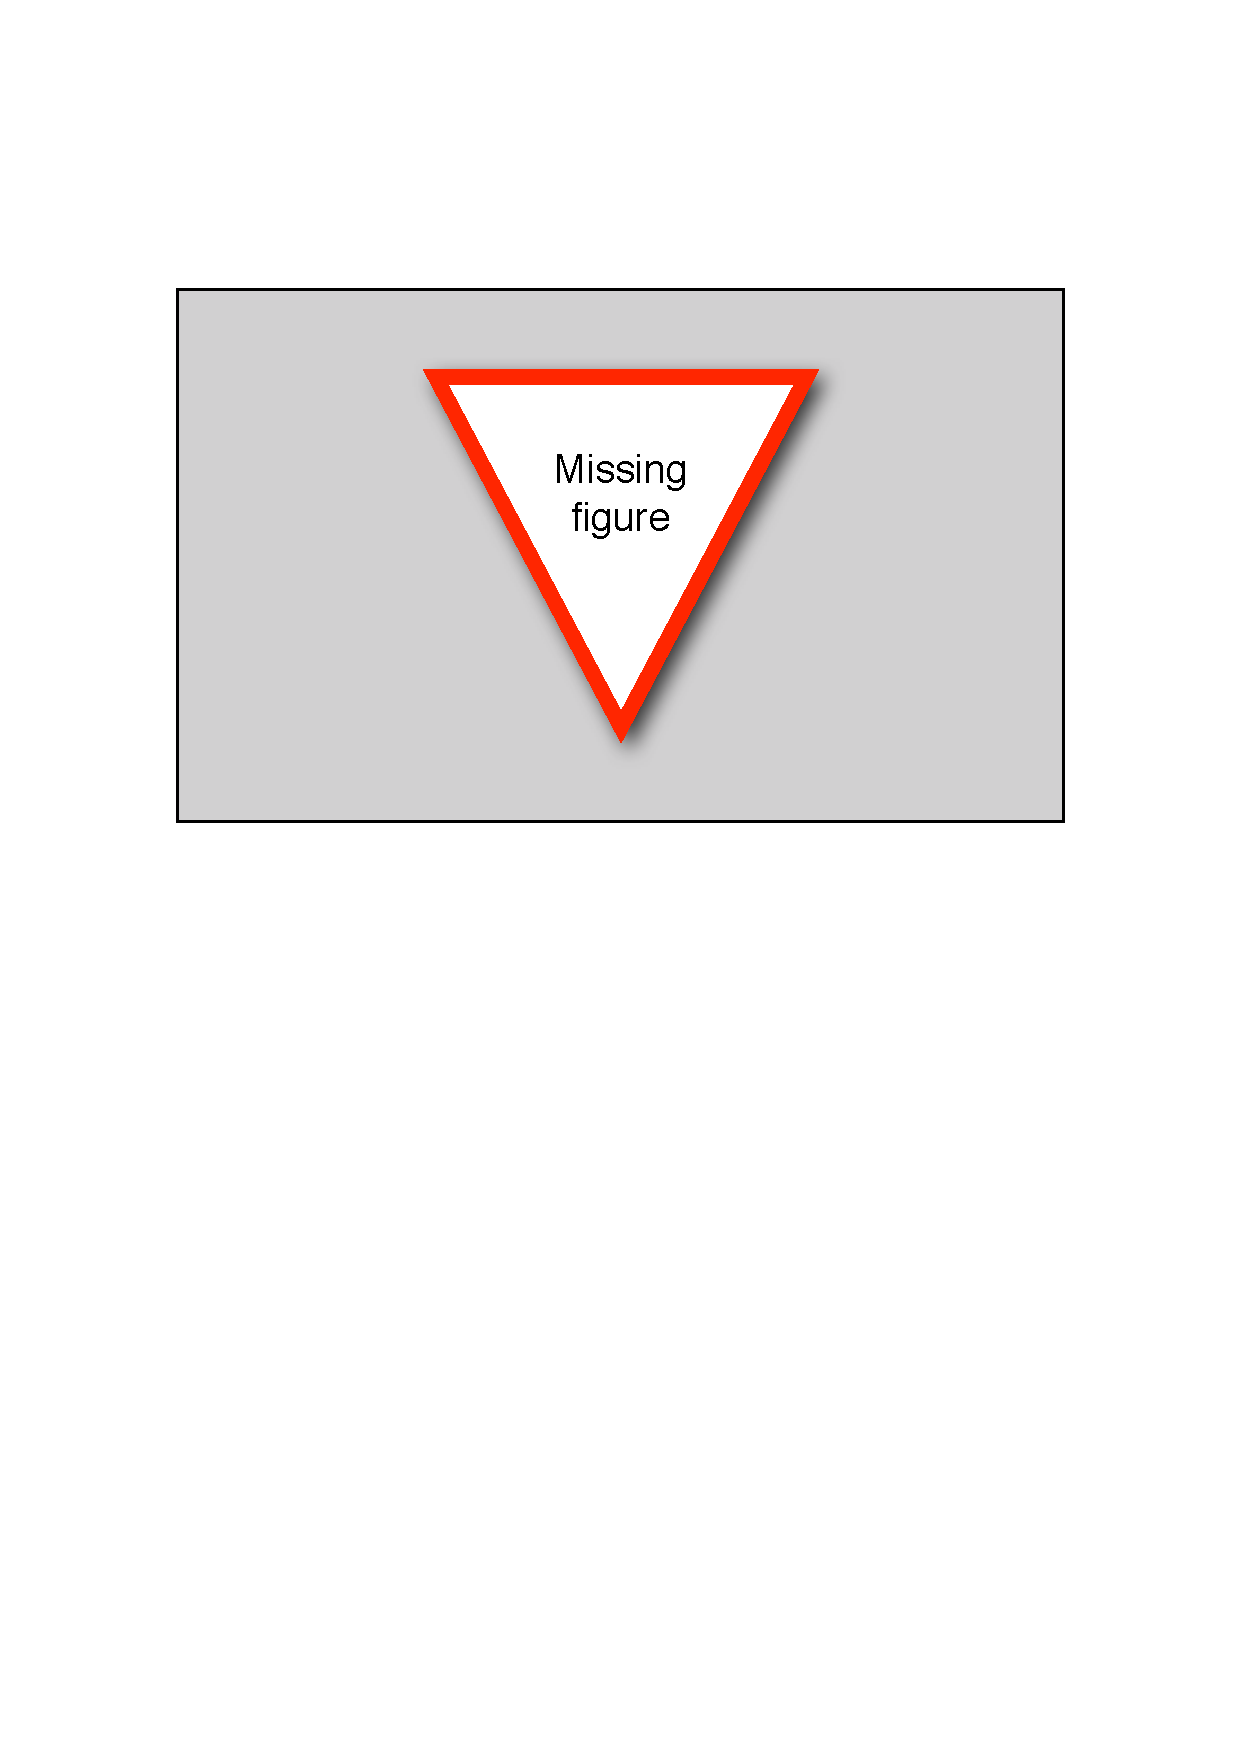
\includegraphics[width=\size]{images/MissingFigure}
			          \caption{\textbf{\textcolor{red}{Missing Figure \themissingFigureCount}} - #4}
			          \label{fig:#5}
		        \end{center}
	        \end{figure}
        \case{\isequal{#1}{real}}
           \begin{figure}[#3]
    		      \begin{center}
			          \includegraphics[width=\size]{images/#6}
			          \caption{#4}
			          \label{fig:#5}
		        \end{center}
	        \end{figure}
        \otherwise
            \begin{center}
                \textbf{\textcolor{red}{FIGURE $\Rightarrow$ No Tag Match !!}}
            \end{center}
    \endswitch
}



%-------------------------------------------------------------------------
% Trennung
%-------------------------------------------------------------------------
%---------------------------------------------------------------------------------------------------
% Trennung
% Hier können alle Wörtertrennungen definiert werden. Die nachfolgenden dienen als Beispiel
% und wurden aus der Vorlage von Michael Knop übernommen.
%---------------------------------------------------------------------------------------------------
\hyphenation{Web-ap-pli-ka-tion Web-ap-pli-ka-tio-nen Web-an-wen-dung Web-an-wen-dung-en My-SQL Kon-text-in-for-ma-ti-onen}

%-------------------------------------------------------------------------
% Anpassung der Parameter, die TeX bei der Berechnung der Zeilenumbrüche verwendet:
%-------------------------------------------------------------------------
\tolerance 1414
\hbadness 1414
\emergencystretch 1.5em
\hfuzz 0.3pt
\widowpenalty=10000
\vfuzz \hfuzz
\raggedbottom


%-------------------------------------------------------------------------
% Meine Pakete:
%-------------------------------------------------------------------------
\setlength {\marginparwidth }{2cm}
\usepackage{todonotes}

\usepackage{caption}
\usepackage{subcaption}
\usepackage{boolexpr,pdftexcmds,trace}
%-------------------------------------------------------------------------
%\usepackage[
    %a4paper,
    %left = 3cm,
    %right = 1.0in,
    %top= 1in,
    %bottom = 0.8in    
%]{geometry}
%\usepackage{showframe} % Show page margin
%-------------------------------------------------------------------------
\usepackage{enumitem}
\usepackage{amsmath}
\usepackage{mathrsfs}
\usepackage{amssymb}
\parindent0pt % do not indet line after new line
\usepackage{trfsigns} % For transformation signs

\usepackage[
    format=hang,
    labelfont=bf,
    textfont=normalfont,
    justification=justified
]{caption}

\usepackage{float} % To force figure position in desired place, use specifier H
\usepackage{cancel}

%-------------------------------------------------------------------------
% Define listing colors
\usepackage{color}
\definecolor{backgroundcolor}{gray}{0.95}
\definecolor{keywordcolor}{cmyk}{0.3,0.76,0,0}
\definecolor{stringcolor}{cmyk}{0.2,0.89,0.97,0.04}
\definecolor{numbergcolor}{cmyk}{0.84,0.64,0,0}
\definecolor{commentgcolor}{cmyk}{0.70,0.14,0.96,0.39}

% Define listing font
% \usepackage[scaled=0.85]{luximono}

% Define listing prperties
\usepackage{listings}
\lstset{
language = C,
numbers=left,
numberstyle=\footnotesize \ttfamily,
stepnumber=1,
numbersep=5pt,
frame=single,                   % adds a frame around the source code
framexleftmargin=8mm,
backgroundcolor=\color{backgroundcolor},
xleftmargin = 0.9cm,
linewidth = \textwidth,
aboveskip = 0.5cm,
%belowskip = 0.5cm,
breaklines = true,
breakatwhitespace = true,
tabsize=2,
basicstyle=\footnotesize \ttfamily,
keywordstyle=\color{keywordcolor}\textbf \ttfamily,
stringstyle=\color{stringcolor}\ttfamily,
commentstyle=\color{commentgcolor}\small \ttfamily,
numberstyle=\tiny,
abovecaptionskip=10pt,
captionpos=b
escapeinside={(*@}{@*)},	% if you want to add a comment within your source code
morekeywords={*,...}     	% if you want to add more keywords to the set
}

\renewcommand{\lstlistlistingname}{Quelltextverzeichnis}
\renewcommand{\lstlistingname}{Quelltext}
%-------------------------------------------------------------------------





					% Die stilistischen Parameter

%--------------------------------------------------------------------------
% Anfang des Schriftstücks
%--------------------------------------------------------------------------

\begin{document}

%--------------------------------------------------------------------------
% Titelseite
%--------------------------------------------------------------------------
\begin{titlepage}
	\begin{center}

		\vspace*{2cm}
		\huge
		\textbf{Acoustic localisation of a speaker source in a reverberant environment}

		\vspace{2.5cm}
		\large
		\textbf{Mathias Buder}

		\vspace{0.25cm}
		\small
		\textnormal{mathias.buder@gmail.com}
		

		\vspace{3 cm}

		\textbf{Zusammenfassung}

	\end{center}

In der vorliegenden Arbeit erfolgt die Entwicklung eines Echtzeitsystems zur
räumlichen Detektion einer Sprachquelle unter Verwendung eins kugelförmigen
Mikrofonarrays. Die gesamte im Vorfeld durchgeführte Simulation wurde dabei
mit der Entwicklungsumgebung MATLAB R realisert. Die im zweiten Teil beschriebene Echtzeitimplementierung erfolgte auf Basis des D.Module.C6713 in
der Programmiersprache C.

\end{titlepage}

%--------------------------------------------------------------------------
% Verzeichnisse
%--------------------------------------------------------------------------
	% \listoftodos									% ToDo-Verzeichnis
	\tableofcontents								% Inhaltsverzeichnis
	\listoftables									% Tabellenverzeichnis
	\listoffigures									% Abbildungsverzeichnis
	\lstlistoflistings
%--------------------------------------------------------------------------
% Teile
%--------------------------------------------------------------------------

	%\newpage

% ****************************************************************************************
\chapter{Einführung}
\label{chap:Einfuehrung}
% ****************************************************************************************



%\pagebreak

% ****************************************************************************************
\section{Problemformulierung}
\label{sec:Problemformulierung}
% ****************************************************************************************
Die vorliegende Arbeit beschäftigt sich mit dem Design, der Simulation sowie der Implementierung eines digitalen Echtzeitsystems zur Lokalisierung einer bewegten Sprachquelle innerhalb eines geschlossenen Raumes. Ziel ist die Erstellung eines Algorithmus, der auf Basis geeigneter Schätzverfahren die Richtung (Horizontal- und Vertikalwinkel) dieser Signalquelle, bezogen auf ein Referenzkoordinatensystem, ermittelt (\abb{Sprecher_In_Raum}). Als zugrunde liegendem theoretischen Ansatz zur Bestimmung der Schalleinfallsrichtung (DOA\footnote{Direction-Of-Arrival}) eines Quellensignals werden hier die Laufzeitunterschiede (TDOA\footnote{Time-Difference-Of-Arrival}) zwischen den einzelnen Mikrofonen sowie die bekannte Geometrie der Mikrofonanordnung\footnote{Mikrofonarray} ausgenutzt. Eine graphische Darstellung soll letztlich mittels serieller Übertragung der geschätzten Ergebnisse an ein Anzeigegerät realisiert werden.

% ------------------------------------------ FIGURE --------------------------------------
\myFigure{real}
         {big}
         {htbp}
         {Richtungsbestimmung einer bewegten Sprachquelle im Raum.}
         {Sprecher_In_Raum} 
         {01_Einfuehrung/Sprecher_In_Raum}
% ------------------------------------------ FIGURE --------------------------------------

Zur Lösung diese Aufgabenstellung stehen ein kugelförmiges Mikrofonarray mit acht Kondensatormikrofonen (\abb{Foto_MikrofonArray}) inkl. Mikrofonvorverstärker, ein leistungsstarker digitaler Signalprozessor (\abb{Foto_DSP}) der Firma \ti sowie ein Desktopcomputer zur Verfügung.

% ----------------------------------------- SUB-FIGURE -----------------------------------
\begin{figure}
        \centering
        \begin{subfigure}[b]{0.435\textwidth}
                \centering
                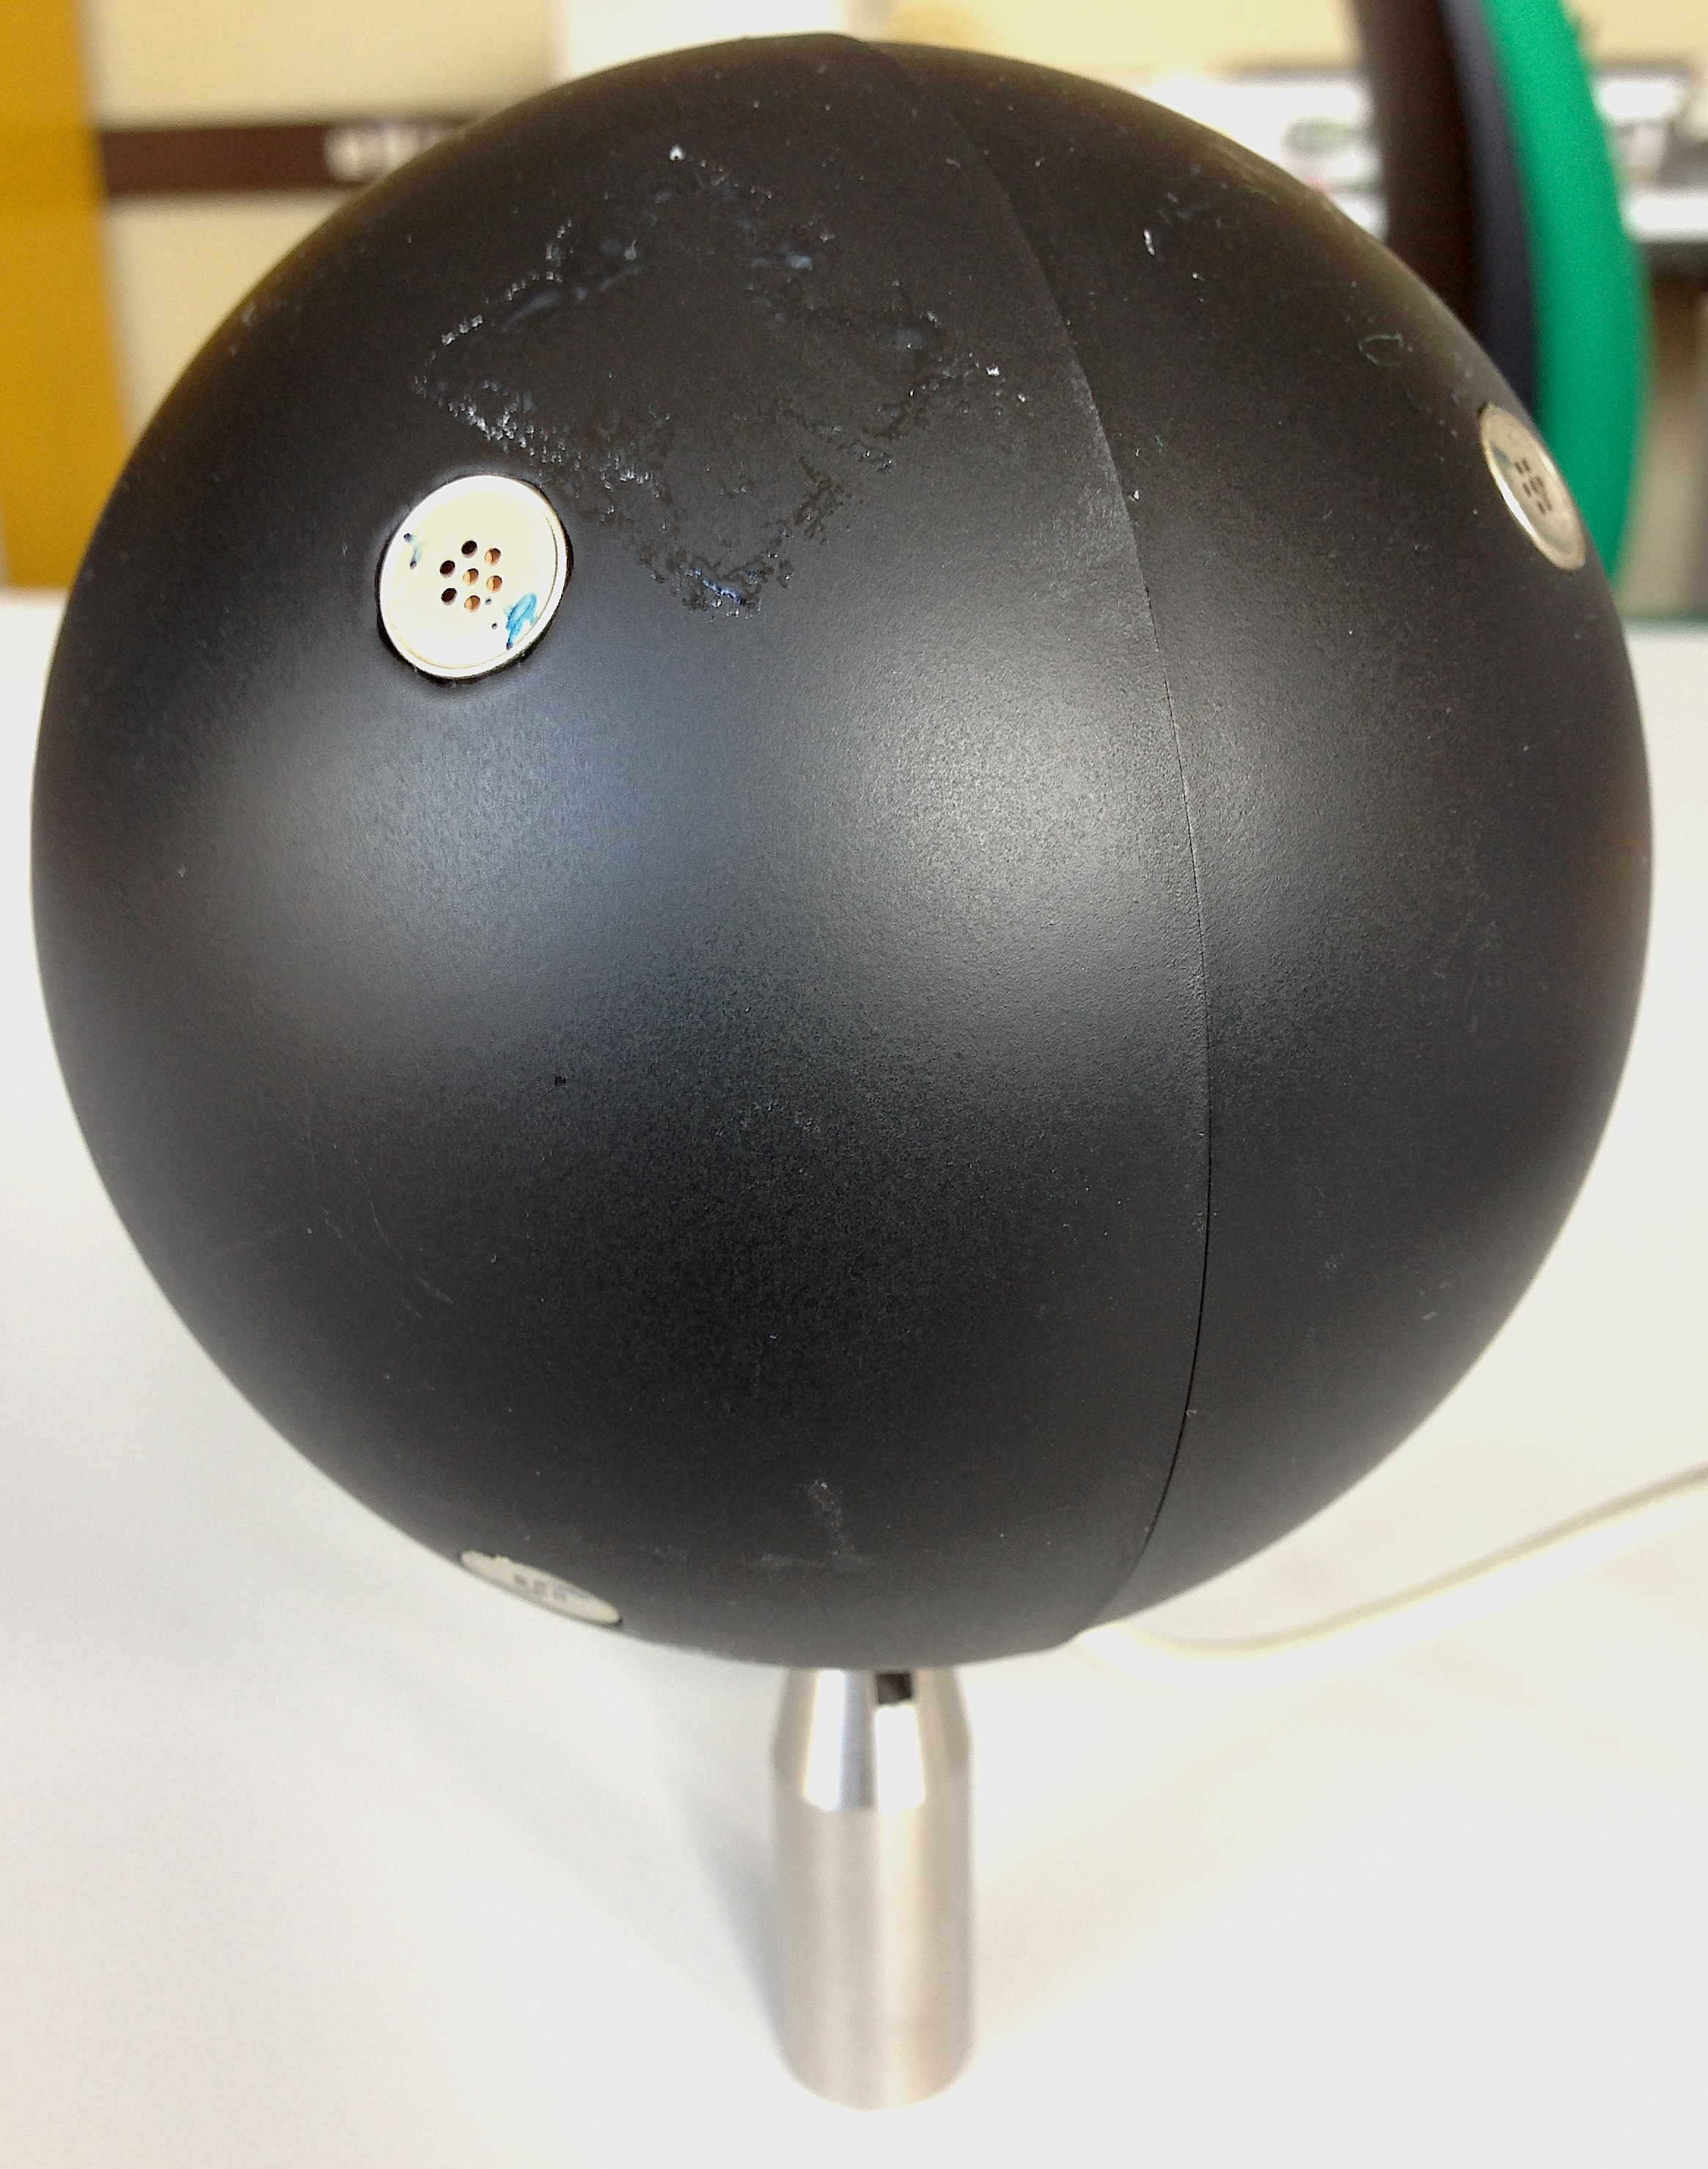
\includegraphics[width=\textwidth]{images/01_Einfuehrung/Foto_MikrofonArray}
                \caption{kugelförmiges Mikrofonarray}
                \label{fig:Foto_MikrofonArray}
        \end{subfigure}
        ~ %add desired spacing between images, e. g. ~, \quad, \qquad etc.
          %(or a blank line to force the subfigure onto a new line)
        \begin{subfigure}[b]{0.48\textwidth}
                \centering
                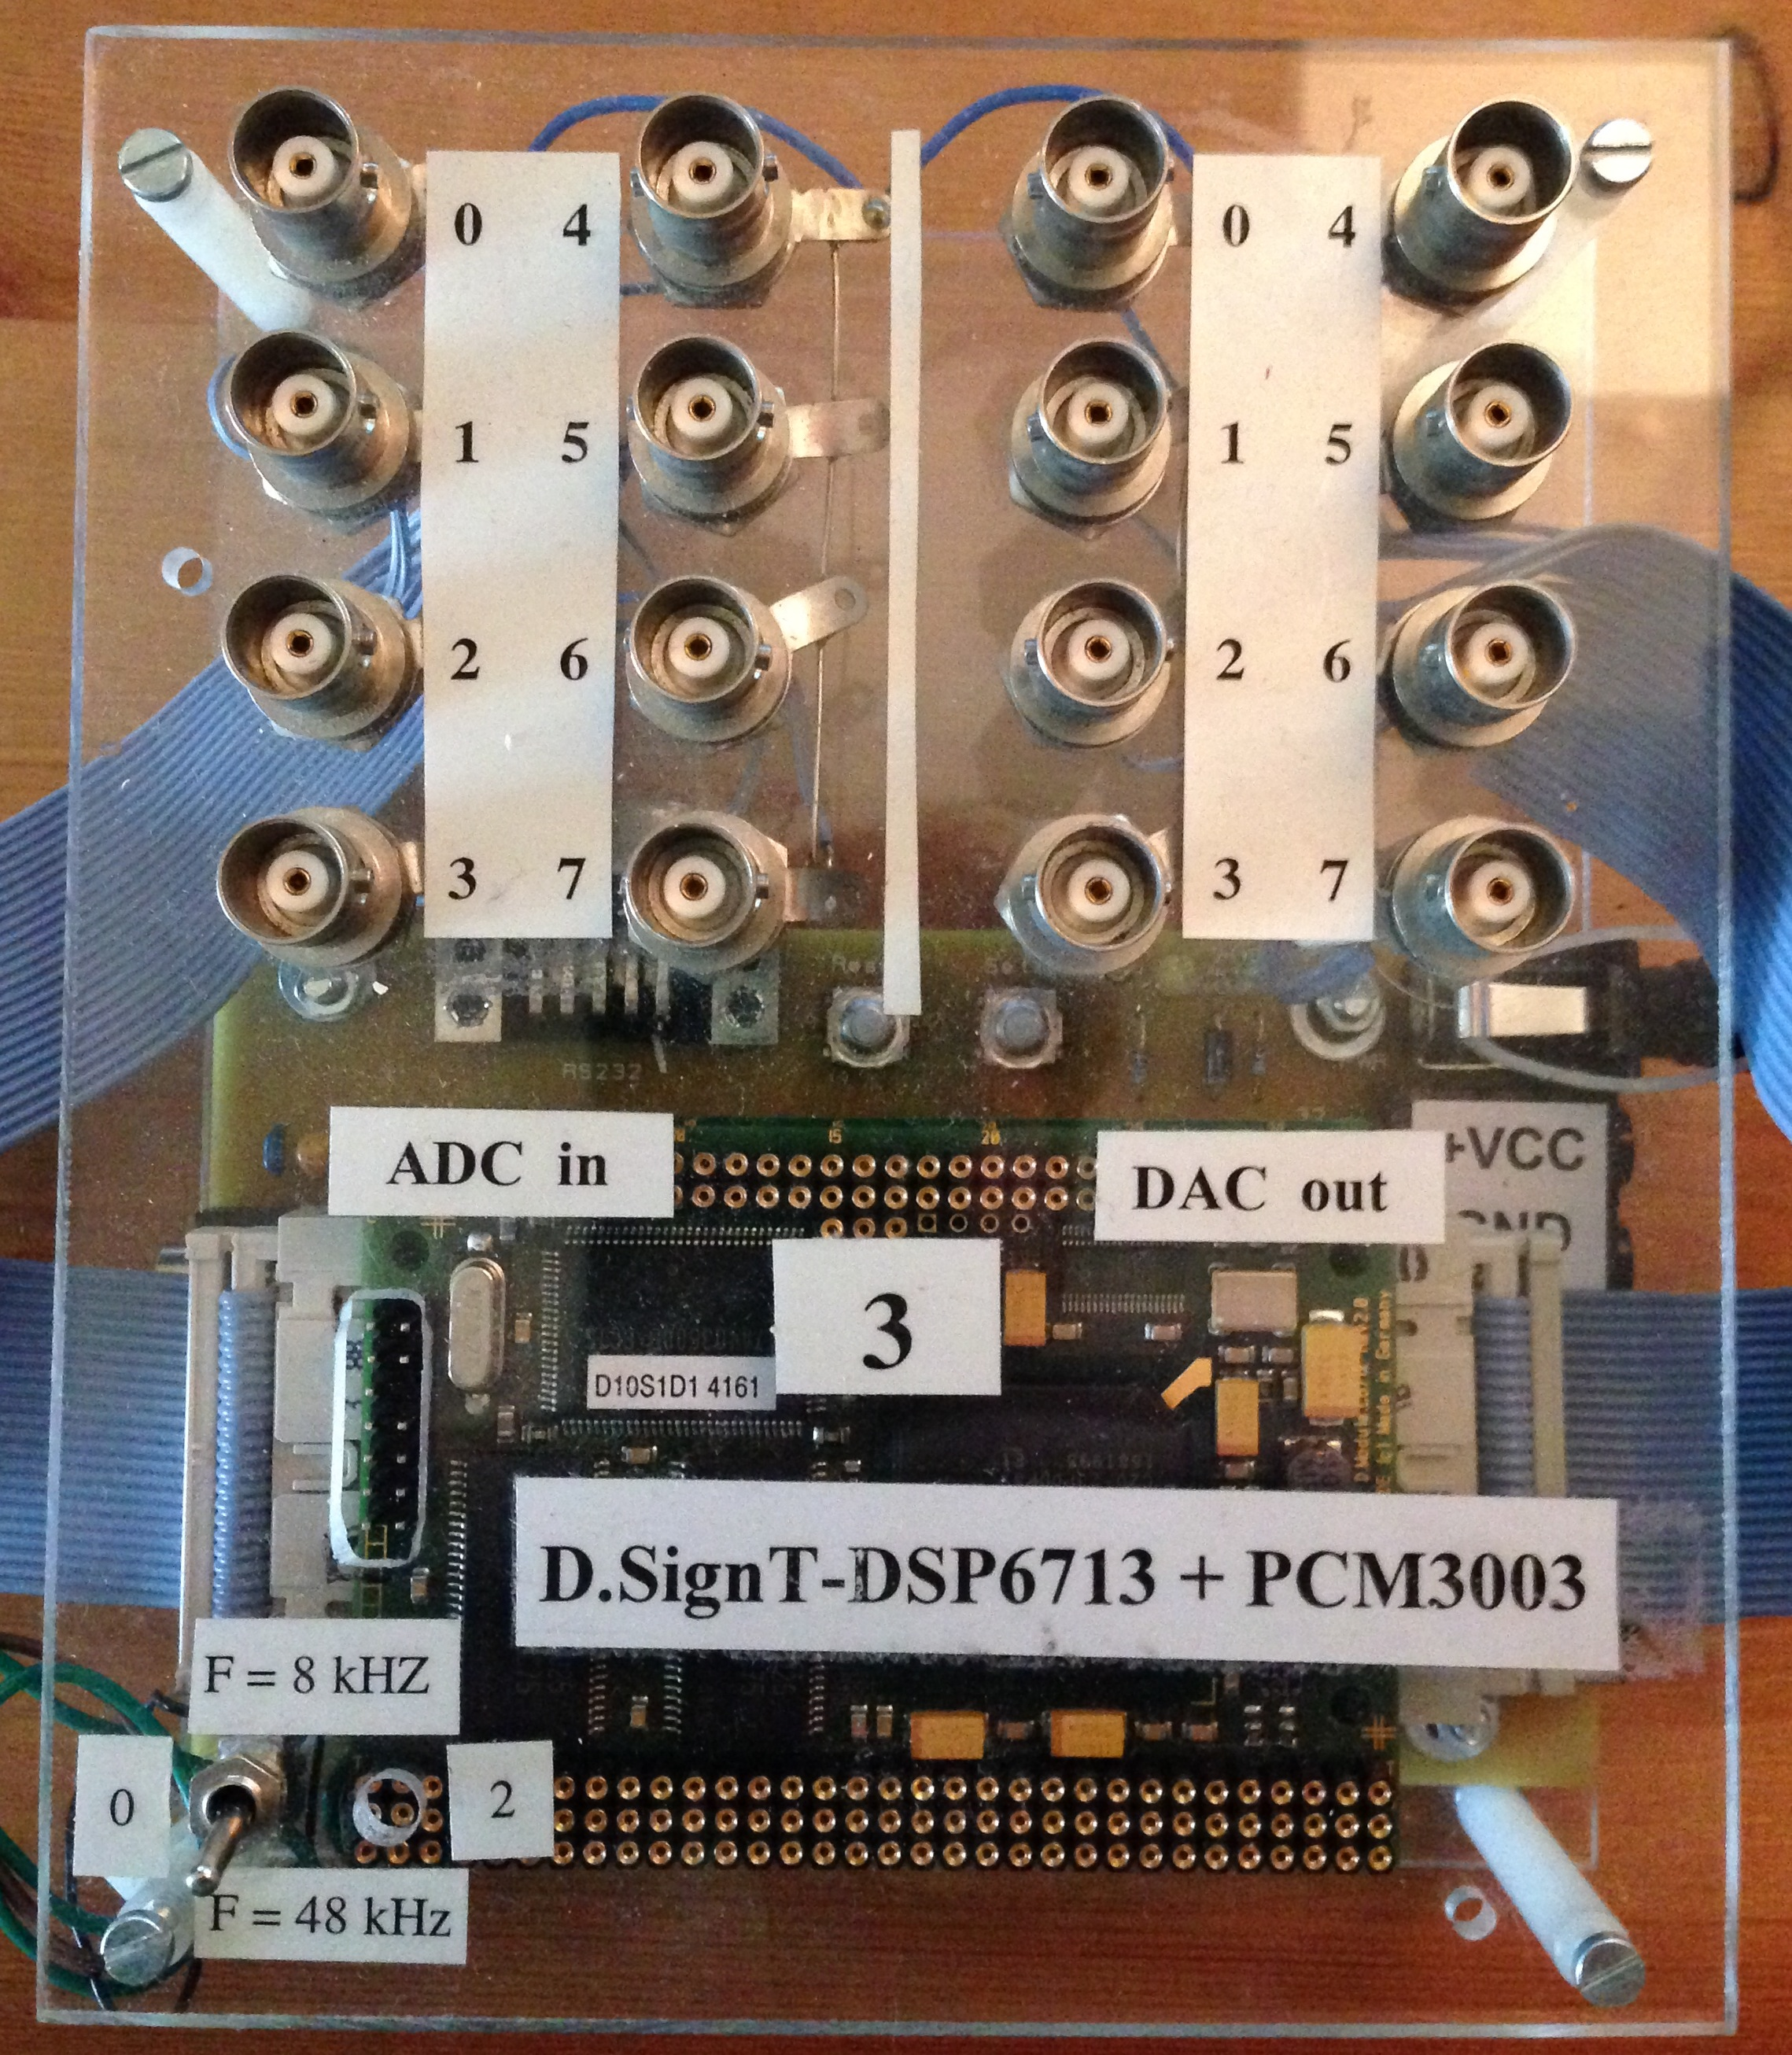
\includegraphics[width=\textwidth]{images/01_Einfuehrung/Foto_DSP}
                \caption{Digitaler Signalprozessor}
                \label{fig:Foto_DSP}
        \end{subfigure}
        \caption{Verwendete Hardware}
        %\caption{Verwendete Hardware}
\end{figure}
% ----------------------------------------- SUB-FIGURE -----------------------------------



\abb{Blockschaltbild_System} zeigt ein Prinzip-Blockschaltbild des Systems. Dieses lässt sich wie dargestellt in einen analogen -und digitalen Systemabschnitt klassifizieren. Im Rahmen dieser Arbeit soll die Signalverarbeitung im digitalen Systemabschnitt im Vordergrund stehen, da bereits alle Komponenten des Analogabschnitts funktionsfähig zur Verfügung gestellt wurden.

Die Ergebnisse dieser Arbeit wurden auf Basis von \citet{Master_Array_Pikora}, \citet{Master_Array_Mueller} sowie des in \citet[S. 196ff]{Book_Array_Benesty} und \citet{Paper_Array_Benesty} beschriebenen Verfahrens des Mehrkanal-Kreuzkorrelationskoeffizienten (MCCC\footnote{Multichannel Cross-Correlation Coeffcient}) erzielt.


% ------------------------------------------ FIGURE --------------------------------------
\myFigure{real}
         {max}
         {htbp}
         {Blockschaltbild des Detektionssystems}
         {Blockschaltbild_System} 
         {01_Einfuehrung/Blockschaltbild_System}                                
% ------------------------------------------ FIGURE --------------------------------------

% Die Richtungsinformation der Quelle kann so unter Berücksichtigung der geometrische Zusammenhänge zwischen Schallwelle und Mikrofonarray aus der Laufzeitdifferenz zwischen den Mikrofonen extrahiert sowie auf ein beliebiges Koordinatensystem abgebildet werden.



% Hier noch was zum Koordinatensystem, den beiden Winkeln und absolute position des Arrays, fernfeld usw. schreiben.


% ****************************************************************************************
\section{Zielsetzung}
\label{sec:Zielsetzung}
% ****************************************************************************************
Auf Basis der unter \Sec{sec:Problemformulierung} genannten Problemstellung lassen sich folgende vom System zu erfüllende Ziele definieren:

\begin{enumerate}
    \item Fähigkeit zur Verarbeitung breitbandiger Signale wie Sprache
    \item Fähigkeit zur räumlichen Richtungsdetektion der Quelle mit ausreichend hoher Genauigkeit (Horizontal- sowie Vertikalwinkel)
    \item Fähigkeit zum Einsatz in Umgebungen mit hohem Rauschanteil und/oder Reflexionsfaktor
    \item Fähigkeit zur Datenverarbeitung in Echtzeit
\end{enumerate}

Der Begriff "`Echtzeit"' lässt sich dabei wie folgt definieren: \\

\definition{Ein Programm rechnet in Echtzeit, wenn es Eingabedaten so schnell verarbeitet, wie der Vorgang, der sie erzeugt. \cite[S. 34]{Slide_ImageProcess_Koelzer}}


Im Hinblick auf eine spätere Implementierung mit Verwendung eines digitalen Signalprozessors lassen sich aus den oben genannten Zielen folgende Forderungen spezifizieren, um eine ordnungsgemäße Funktion des Gesamtsystems zu gewährleisten:

\begin{enumerate}
    \item Verarbeitung von Sprachsignalen bis zu einer oberen Grenzfrequenz von $f_{max} = 3 kHz$
    \item Robustes Verfolgen einer Sprachquelle innerhalb eines definierten Winkelraums:
        \begin{itemize}[label = \textbullet]
            \item Azimuth: $0° \leq \theta < 360°$
            \item Elevation: $-90° < \phi < 90°$
        \end{itemize}
    \item Die Dauer der Datenverarbeitung muss gleich oder kleiner der Datenaufzeichnungsdauer sein. Demzufolge muss die Bedingung $T_{Processing} \leq T_{Frame}$ dauerhaft erfüllt sein.
    \item Der Prozess von Datensammlung und Datenverarbeitung muss zwingend nebenläufig stattfinden.
    \item Zur Sicherstellung der Ergebniskontinuität muss ein kontinuierlicher Datenstrom zwischen Ein- und Ausgabeschnittstelle gewährleistet sein. 
\end{enumerate}


	% ****************************************************************************************
\chapter{Konzeptionierung}
\label{chap:Konzeptionierung}
% ****************************************************************************************
Die grundlegenden Prinzipien und die daraus resultierenden Verfahren der Signalverarbeitung unter Verwendung von Mikrofonarrys sind ein essentieller Bestandteil dieser Arbeit. Es ist somit zwingend notwendig, die damit verbundenen mathematischen Zusammenhänge sowie die daraus abgeleiteten Methoden zu verstehen und gezielt einsetzen zu können.

Im folgenden Kapitel werden zunächst die elementaren Größen und Modelle der Array Signalverarbeitung eingeführt. Bezogen auf diese Grundlagen erfolgt anschließend der Entwurf eines mathematischen Modells zur Lösung der unter \Sec{sec:Problemformulierung} beschriebenen Problemstellung.

% ****************************************************************************************
\section{Grundlegende Annahmen und deren mathematische Zusammenhänge}
\label{sec:AnnahmenUndMatheZusammenhaenge}
% ****************************************************************************************
Im folgenden werden die System- sowie Signaleigenschaften des hier vorliegenden Systems untersucht. Die zu verarbeitenden Signale werden im weiteren Verlauf als Quellensignal und das von den Mikrofonen gelieferte als Sensorsignal bezeichnet.


% ****************************************************************************************
\subsection{System- und Signalmodell}
\label{subsec:Systemmodell}
% ****************************************************************************************
% Zunächst Beschreibung des SIMO - Systems mit Impulsantwort. Dann beschreiben, dass es sich um eine verzerrungsfreies System handelt da gilt y_n(t) = a_n * x_n(t-tau_n) (eigentlich entstehen nur lineare Verzerrungen, Dämpfung und Verzögerung)
% siehe script_ST1_v2.pdf Seite 40

\abb{IllustrationMikrofonarraySystems_a} illustriert den grundlegenden Aufbau eins Mikrofonarray Systems. Dieses besteht aus einem Quellensignal $s(k)$ sowie aus $N+1$ Sensorsignalen $y_n(k)$ die jeweils über eine der $N+1$ Kanalimpulsantworten $g_n$ mit dem Quellensignal verknüpft sind. Solch eine Signalkonstellation wird als SIMO\footnote{single-input multiple-output}-Modell \cite[S. 141]{Book_Array_Benesty} bezeichnet und kann durch folgende Gleichung beschrieben werden


\begin{equation}
\label{eq:SIMO}
    y_n(k) = g_{n} \ast s(k) + v_n(k)
\end{equation}

wobei $v_n(k)$ das dem Signal additiv überlagerte Umgebungsrauschen darstellt.


%\begin{align}
%        \mathbf{s}(k) & = \left[ s(k)~s(k-1) \cdots s(k-L_g+1)\right]^T \\
%        \mathbf{g}_N & = \left[ g_{N0}~g_{N1} \cdots g_{NL_g-1}\right]^T
%\end{align}


%Der Parameter $Lg$ steht dabei für die Länge der längsten Impulsantwort und $v(k)$ für das dem Signal additiv überlagerte Umgebungsrauschen.  



% ----------------------------------------- SUB-FIGURE -----------------------------------
\begin{figure}
        \centering
        \begin{subfigure}[b]{0.48\textwidth}
                \centering
                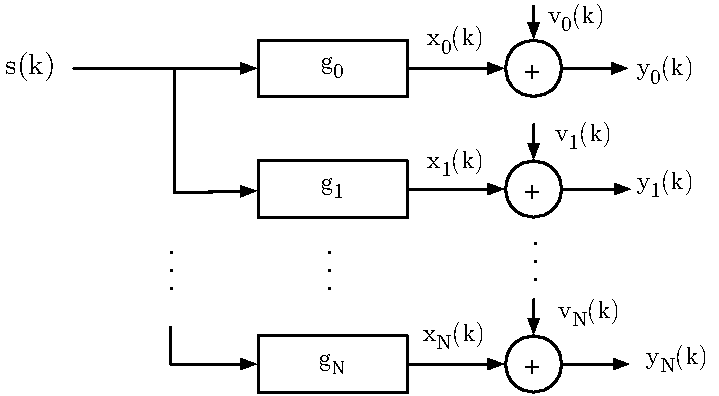
\includegraphics[width=\textwidth]{images/02_Konzeptionierung/IllustrationMikrofonarraySystem_a}
                \caption{}
                \label{fig:IllustrationMikrofonarraySystems_a}
        \end{subfigure}
        ~ %add desired spacing between images, e. g. ~, \quad, \qquad etc.
          %(or a blank line to force the subfigure onto a new line)
        \begin{subfigure}[b]{0.48\textwidth}
                \centering
                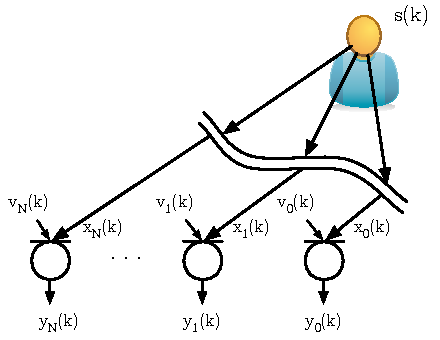
\includegraphics[width=\textwidth]{images/02_Konzeptionierung/IllustrationMikrofonarraySystem_b}
                \caption{}
                \label{fig:IllustrationMikrofonarraySystems_b}
        \end{subfigure}
        \caption{Illustration des Mikrofonarray Systems}
        %\caption{Verwendete Hardware}
\end{figure}
% ----------------------------------------- SUB-FIGURE -----------------------------------

Bei genauerer Untersuchung von \abb{IllustrationMikrofonarraySystems_b} können über die vom System verursachte Transformation des Quellensignals $s(k)$ in das Sensorsignal $y_n(k)$, unter Berücksichtigung von akustischen Freifeldbedingungen\footnote{ohne jegliche Reflexionen, nur der direkte Ausbeitungspfad wird betrachtet}, folgende Aussagen getroffen werden:


\begin{itemize}
    \item $s(k)$ wird durch die Entfernung von der Signalquelle zu den Sensoren um den Faktor $\alpha_n$ gedämpft/skaliert. Es gilt dabei: $0 \leq \alpha_n \leq 1$
    \item $s(k)$ wird durch die Entfernung zwischen der Signalquelle und den Mikrofonarray um eine Schallausbreitungszeit $T_S$ verzögert 
    \item $s(k)$ wird durch die Entfernung $d$ zwischen den einzelnen Sensoren um eine relative Zeit $\tau_{0n}$ verzögert. $\tau_{0n}$ bezieht sich dabei auf das Referenzmikrofon $M_0$.
     
\end{itemize}

Unter diesen Annahmen lässt sich $y_n(k)$ wie folgt ausdrücken

\begin{equation}
    y_n(k) = \alpha_n s(k - T_S- \tau_{n1}).
\end{equation}

%Bei $n=0$ folgt für die Laufzeiten $\tau_{n1} = 0$ und $T_n = t_S$.
Aus dieser Erkenntnis, dem in \Eq{SIMO} gezeigten Zusammenhang und der Vernachlässigung des additiven Rauschens $v(t)$ können die Kanalimpulsantworten $g_n$ wie folgt gefunden werden:

\begin{equation}
     \alpha_n s(k - T_S- \tau_{n0}) = \underbrace{\alpha_n \delta(k - T_S- \tau_{n0})}_{g_n} ~ \ast ~  s(k)
\end{equation}

Zur Ermittlung des Systemverhaltes ist es zwingend notwendig genaue Kenntnis über den Frequenz- und Phasengang zu erlangen. Diesen erhält man durch Fouriertransformation der $N+1$ Impulsantworten $g_n$.

\begin{equation}
g_n = \alpha_n \delta(k - T_S - \tau_{n1}) \hspace{0.5cm} \laplace \hspace{0.5cm} \underline{G}_n(\e^{\im \omega}) = \alpha_n \e^{-\im \omega (T_s + \tau_{n0})} \hspace{0.5cm} \text{für} \hspace{0.5cm} n=1 \dots N
\end{equation}


Der gewünschte Amplituden- und Phasengang lässt sich nun direkt aus dem komplexen Frequenzgang $\underline{G}_n(\e^{\im \omega})$ ablesen.



\begin{equation}
    \begin{array}{rrl}
  \text{\textbf{Amplitudengang:}} &
  \left | \underline{G}_n(\e^{\im \omega}) \right | & = \alpha_n \\
    \text{\textbf{Phasengang:}} &
    \varphi_n(f) & = - 2 \pi f (T_s + \tau_{n0})
   \end{array}
  \label{eq:SystemEigenschaften}
\end{equation}
 

Aus dem Frequenzgang leitet sich ein konstanter Amplitudengang $\alpha_n$ (Dämpfungsverzerrung) sowie ein frequenzproportionaler Phasengang (Phasenverzerrung) $-2 \pi f  (T_s + \tau_{n0}) \sim f$ ab. Diese Systemeigenschaft lässt sich direkt einem idealen verzerrungsfreien LTI\footnote{Linear Time Invariant}-System zuordnen \cite[S. 63ff]{Book_SignalTransmission_Kammayer}. Das hier zu implementierende reale System muss das in \Eq{SystemEigenschaften} dargestellte Verhalten innerhalb der Signalbandbreite möglichst gut approximieren.




% ****************************************************************************************
%\subsection{Signalmodell}
%\label{Subsec:Signalmodell}
% ****************************************************************************************
%\todo[inline]{Beschreibung des Signalmodels wie im Buch von Benisty
%sowie Einführung der Variablen,Single-Source reverberant model, MIMO-System}
%\missingfigure{Ein erklärendes Bild zum Signalmodel - Sprecher, Sensoren, Echo, Rauschen \dots}

% ****************************************************************************************
\subsection{Sensormodell}
\label{subsec:Sensormodell}
% ****************************************************************************************

% ****************************************************************************************
\subsubsection{Lineares zweidimensionales Sensorarray}
\label{subsubsec:linearesArray}
% ****************************************************************************************
\abb{SensormodellLinearenArrays} zeigt den Aufbau eines linearen äquidistanten Mikrofonarrays (ULA\footnote{Uniform Linear Array}) mit einer Anzahl von $N+1$ Sensoren und dem Sensorabstand $d$. Bei einer solchen Anordnung legen die Schallwellen, abhängig vom Schalleinfallswinkel $\theta$ unterschiedlich lange Wege von der Signalquelle zu den einzelnen Sensoren zurück. Unter Berücksichtigung einer ebenen Wellenfront sowie einer bekannten Arraygeometrie lässt sich mit Hilfe der Laufzeitdifferenz $\tau_{ULA}$ und der Schallgeschwindigkeit\footnote{Approximierte Geschwindigkeit bei einer Raumtemperatur von 20°C} $c \approx 343 \frac{m}{s}$ folgender Zusammenhang definieren

\begin{equation}\label{eq:ULA_1}
    \tau_{ULA}= \frac{d}{c} \cdot \cos(\theta)
\end{equation}

Für den hier beschriebenen Fall kann die Laufzeitdifferenz zwischen Referenzsensor $M_0$ und Sensor $M_N$ durch die lineare Funktion $f_{0n,ULA}(\tau)$ ausgedrückt werden


\begin{equation}\label{eq:ULA_2}
    f_{0n,ULA}(\tau) = n \cdot \tau_{ULA} \eqspace \text{mit} \eqspace n=1,2, \dots N
\end{equation}


%Zur Berechnung der Laufzeitdifferenzen zwischen allen Sensorpaarkombinationen $M_{01}, M_{02}, \dots, M_{0N},M_{12}, M_{13} \dots,  M_{(N-1)N}$ kann ebenfalls der lineare Zusammenhang aus \Eq{ULA_2} genutzt werden. Bei einer Anzahl von $N$ Sensoren ergeben sich somit $\frac{N+1}{2} \cdot N$ Laufzeiten.



\myFigure{real}                                      % Figure tag (missing, real)
         {big}                                       % Size (small,medium,big)
         {h}                                         % z.B. htbp
         {Sensormodell eines linearen Arrays}        % Figure title
         {SensormodellLinearenArrays}                % Figure label 
         {02_Konzeptionierung/ULA}                   % Path to real figure
         

% ****************************************************************************************
\subsubsection{Dreidimensionales Sensorarray}
\label{subsubsec:3DArray}
% ****************************************************************************************
Zur räumlichen Detektion einer Schallquelle ist es notwendig eine Sensorgeometrie zu finden, in der die Richtungsinformation durch den Azimuthwinkel $\theta$ sowie den Elevationswinkel $\phi$ ausgedrückt werden kann. Eine solches Array lässt sich mit Hilfe einer Matrix $\mathbf{M}$ repräsentieren, wobei jede Spalte die Position eines der $N+1$ Sensoren in einem dreidimensionalen euklidschen Raum beschreibt. 

\begin{equation}
    \mathbf{M}_{3 \times N+1} = 
    \begin{bmatrix}
        m_{x_0} & m_{x_1} & \dots & m_{x_N} \\
        m_{y_0} & m_{y_1} & \dots & m_{y_N} \\
        m_{z_0} & m_{z_1} & \dots & m_{z_N} \\
    \end{bmatrix}
\end{equation}



%Die erste Spalte dieser Matrix stellt dann den Referenzsensor dar und kann als Zentrum dieses dreidimesionalen Raums betrachtet werden.
\abb{3D_Array_Prinzip_1} zeigt den Referenzsensor im Zentrum dieses Raumes mit einem aus einer beliebigen Richtung eintreffenden Signal. Dieses Signal kann über den Einheitsvektor $\mathbf{s}$, welcher senkrecht zur von der Quelle Emittierten ebenen Wellenfront steht, beschrieben werden. Im Hinblick auf eine spätere Extraktion der oben genannten Raumwinkel wird $\mathbf{s}$ in Kugelkoordinaten ausgedrückt.

\begin{equation}
\textbf{s}_{3 \times 1} =
\begin{bmatrix}
        s_x \\
        s_y \\
        s_z\\
    \end{bmatrix}
    =
    \begin{bmatrix}
        \cos{(\phi)} \cos{(\theta)} \\
        \cos{(\phi)} \sin{(\theta)} \\
        \sin{(\phi)}\\
    \end{bmatrix}
\end{equation}

Der Azimuthwinkel kann dabei die Werte $0° \leq \theta < 360°$ und der Elevationswinkel $-90° \leq \phi \leq 90°$ annehmen.


\myFigure{real} % Figure tag (missing, real)
         {small} % Size (small,medium,big)
         {h} % z.B. htbp
         {Beschreibung der Signalquelle im Raum unter Verwendung von Azimuth- und Elevationswinkel.} % Figure title
         {3D_Array_Prinzip_1} % Figure label 
         {02_Konzeptionierung/3D_Array_Prinzip_1}


Als nächster Designschritt folgt der Zusammenhang zwischen dem Schalleinfallswinkeln und der Laufzeitdifferenz der einzelnen Sensorpaare. \abb{3D_Array_Prinzip_2} illustriert ein Sensorpaar, das durch die Spaltenvektoren $\mathbf{m_0}$ und $\mathbf{m_1}$ repräsentiert wird. Der Verbindungsvektor $\mathbf{m_{01}}$ zwischen den Sensoren berechnet sich mit $\mathbf{m_1} - \mathbf{m_0}$.
% und der Einheitsvektor $\mathbf{s}$ kann erneut als die Schalleinfallsrichtung aufgefasst werden. 
Zu beachten ist, dass $\mathbf{s}$ nun in Richtung der Sensoren zeigt und somit gilt $\mathbf{s} = -\left[\cos(\phi) \cos(\theta) ~  \cos(\phi) \sin(\theta) ~ \sin(\phi) \right]^T$. Die zusätzliche Distanz, die der Schall zurücklegen muss, um von Sensor $M_0$ zu $M_1$ zu gelangen wird als Laufwegunterschied $s_{01}$ bezeichnet. Wie in \abb{3D_Array_Prinzip_2} dargestellt ergibt sich $s_{01}$ durch Projektion von $\mathbf{m_{01}}$ mit Bezug auf den Schalleinfallsvektor $\mathbf{s}$.  $s_{01}$ kann somit durch das Skalarprodukt 

\begin{equation}
    s_{01} = \left ( \mathbf{m_1} - \mathbf{m_0} \right )^T \mathbf{s} = \mathbf{m_{01}}^T \, \mathbf{s}
\end{equation}

ermittelt werden. Folglich bildet sich die Laufzeitdifferenz $\tau_{01}$ durch

\begin{equation}
    \tau_{01} = \left[ \mathbf{m_{01}}^T \, \mathbf{s} \right] \cdot c^{-1}
\end{equation}
  
%% ALT
%Zur Bestimmung der Laufzeitdifferenzen zwischen allen $N$ Sensoren muss zunächst eine Matrix $\mathbf{A}$ definiert werden, in der die Verbindungsvektoren $\mathbf{m}$ aller $M = \frac{N}{2} \cdot (N-1)$ Sensorpaarkombinationen definiert sind.

%\begin{equation}
%    \mathbf{A}_{3 \times M} = 
%    \begin{bmatrix}
%        \mathbf{m}_{12} & \mathbf{m}_{13} & \dots & \mathbf{m}_{1N} & \mathbf{m}_{23} & \mathbf{m}_{24} & \dots & \mathbf{m}_{(N-1)N}
%    \end{bmatrix}
%%    =
%%    \begin{bmatrix}
%%        m_{x_{12}} & m_{x_{13}} & \dots & m_{x_{(N-1)N}} \\
%%        m_{y_{12}} & m_{y_{13}} & \dots & m_{y_{(N-1)N}} \\
%%        m_{z_{12}} & m_{z_{13}} & \dots & m_{z_{(N-1)N}}
%%    \end{bmatrix}
%\end{equation}


Zur Bestimmung der Laufzeitdifferenzen zwischen allen Sensoren muss zunächst eine Matrix $\mathbf{A}$ definiert werden, in der die Verbindungsvektoren $\mathbf{m_{0n}}$ aller $N$ Sensorpaarkombinationen definiert sind.

\begin{equation}
    \mathbf{A}_{3 \times N} = 
    \begin{bmatrix}
        \mathbf{m}_{01} & \mathbf{m}_{02} & \dots & \mathbf{m}_{0N}    \end{bmatrix}
%    =
%    \begin{bmatrix}
%        m_{x_{12}} & m_{x_{13}} & \dots & m_{x_{(N-1)N}} \\
%        m_{y_{12}} & m_{y_{13}} & \dots & m_{y_{(N-1)N}} \\
%        m_{z_{12}} & m_{z_{13}} & \dots & m_{z_{(N-1)N}}
%    \end{bmatrix}
\end{equation}



Dabei gilt für $\mathbf{m}_{3 \times 1}$ der Ausdruck

\begin{equation}
    \mathbf{m}_{1N} = 
    \begin{bmatrix}
       x_{0N} \\
       y_{0N} \\
       z_{0N}
    \end{bmatrix}
    =
    \begin{bmatrix}
       x_{N} - x_0 \\
       y_{N} - y_0 \\
       z_{N} - z_0
    \end{bmatrix}
\end{equation}

Die gesuchten Laufzeitdifferenzen können nun in einem Vektor $\boldsymbol{\tau}_{N \times 1}$ beschrieben werden. Für ein statisches Sensorarray sind diese ausschließlich von der Schalleinfallsrichtung und damit von den Winkeln $\phi$ und $\theta$ abhängig.

\begin{equation}\label{eq:DOA_winkel}
    \begin{array}{ll}
        \boldsymbol{\tau}(\phi, \theta)_{N \times 1} & =  \left[ \left( \mathbf{A}^T \right)_{N \times 3} \cdot \mathbf{s}_{3 \times 1} \right]_{N \times 1} \cdot c^{-1} \\
                                                     & = f_n(\phi, \theta) \eqspace \text{mit} \eqspace n = 1,2, \dots, N
    \end{array}
\end{equation}

Ein Sensorarray mit beliebiger Geometrie kann so analog zu \Eq{ULA_2} durch die nicht-lineare Funktion $f_n(\phi, \theta)$ beschrieben werden. Auf Grund einer nicht-quadratischen Matrix $\mathbf{A}$ muss dessen Inverse als Pseudoinverse $\textbf{A}^{+}$ gebildet werden \cite[S. 185]{Book_MatrixTheory_Piziak}. \Eq{DOA_winkel} kann so mit Bezug auf $\boldsymbol{s}$ in

\begin{equation}
        \boldsymbol{\hat s}(\phi, \theta)_{3 \times 1} = \left \{ \left [ \underbrace{\left( \textbf{A} \cdot \textbf{A}^T \right)^{-1} \cdot \textbf{A}}_{\textbf{A}^{+}}  \right]_{3 \times N} \cdot \boldsymbol{\hat \tau}(\phi, \theta)_{N \times 1} \right \}_{3 \times 1} \cdot c  
\end{equation}

umgeformt werden. $\boldsymbol{\hat s}(\phi, \theta)$ beschreibt dabei den geschätzten Normalvektor\footnote{$\boldsymbol{s}$ steht senkrecht zur einlaufenden Wellenfront} zur Schalleinfallsrichtung und $\boldsymbol{\hat \tau}$ die Schätzung der paarweisen Laufzeitdifferenz \cite[S. 71]{Master_Array_Varma}.
 
 
 
\subsubsection{Räumliches Aliasing} 
Basierend auf den Ausführungen zum räumlichen Alias-Effekt in \cite[8 f]{Master_Array_Pikora} ist bei der Dimensionierung des Sensorarrays folgendes Kriterium zu berücksichtigen:
 \begin{equation}\label{eq:raemlichesAliasing}
     d_{min} \leq \frac{\lambda}{2} = \frac{c}{2 f_{max}}
 \end{equation}

 $d_{min}$ ist dabei die geringste Distanz zwischen zwei Sensoren und $f_{max}$ die größte im Signal enthaltene Frequenz.
 
%\todo[inline]{................................................................................................................................}

\myFigure{real} % Figure tag (missing, real)
         {medium} % Size (small,medium,big)
         {h} % z.B. htbp
         {Laufwegdifferenz als Projektionsvetor zwischen zwei Sensoren im Bezug auf den Schalleinfallsvektor $\mathbf{s}$} % Figure title
         {3D_Array_Prinzip_2} % Figure label 
         {02_Konzeptionierung/3D_Array_Prinzip_2}






% ****************************************************************************************        
\subsubsection{Akustisches Fernfeld}
\label{subsubsec:Fernfeld}
% ****************************************************************************************
Zur Sicherstellung einer ebenen Wellenfront muss sich die Signalquelle wie in \abb{MikrofonarrayFernfeld} dargestellt, im akustischen Fernfeld befinden. Unter diesen Umständen darf die von der Quelle emittierte Kugelwelle $s(k)$ auf einem kleinen Bereich linear approximiert werden. Für die Entfernung $r$, von Array bis zu dem Punkt, an dem die Fernfeldbedingung angenommen werden kann muss folgendes gelten\cite[S. 36f]{Book_Audio_Goerne}:

\begin{equation}
    k \cdot r >> 1 \eqspace \text{mit} \eqspace k = \frac{2 \pi}{\lambda} = \frac{2\pi f}{c}
\end{equation}


%\begin{equation}\label{eq:Fernfeld}
%    \hat d _D = \frac{\hat d}{D} = \frac{\kappa}{16\pi} \cdot kD = \frac{\kappa}{8} \cdot \frac{f}{c} \cdot D
%\end{equation}
%
%$\hat d$ beschreibt dabei die Distanz von Signalquelle zu Mikrofonarray, $D$ die größte im Array vorkommende Entfernung zwischen zwei Sensoren und $k$ die Kreiswellenzahl mit
%
%\begin{equation}\label{eq:Kreiswellenzahl}
%    k = \frac{2 \pi}{\lambda} \hspace{0.5cm} \text{und} \hspace{0.5cm} \lambda = \frac{c}{f}
%\end{equation}


\myFigure{real}                  % Figure tag (missing, real)
         {big}                 % Size (small,medium,big)
         {h!}             % z.B. htbp
         {Mikrofonarray im akustischen Fernfeld}                % Figure title
         {MikrofonarrayFernfeld}                % Figure label 
         {02_Konzeptionierung/Fernfeld}     % Path to real figure











%\todo[inline]{Geometrie, Wellenausbreitung (ebene Welle, Fernfeld),
%Koordinatensystem,Mikrofonvektoren, Entwicklung 3D-Arrays wie in
%\texttt{chap2-MIC.pdf}}
%\missingfigure{Ein erklärendes Bild zum Mikrofonmodel, Koordinatensystem,
%Projektion der DOA durch ebene Welle}


% ****************************************************************************************
\section{Schätzverfahren}
\label{sec:Schaetzverfahren}
% ****************************************************************************************
In \Sec{subsec:Sensormodell} wurde gezeigt, dass die Laufzeitdifferenz $\tau$ zwischen den einzelnen Sensorpaaren genutzt werden kann, um mit Hilfe geometrischer Zusammenhänge die Schalleinfallsrichtung zu bestimmen. Da $\tau$ ein unbekannter Parameter ist, kann dieser mit Hilfe geeigneter Verfahren aus mindestens zwei Sensorsignalen geschätzt werden.
Aufgrund der unter \Sec{subsec:Systemmodell} abgeleiteten Systemeigenschaften wie der Verzögerung und Skalierung des Quellensignals durch die Sensorgeometrie kann hier die Kreuzkorrelation als Schätzverfahren angewandt werden.

% ****************************************************************************************
\subsection{Kreuzkorrelation}
\label{subsec:Kreuzkorrelation}
% ****************************************************************************************
Die Kreuzkorrelation zweier kontinuierlicher Funktionen $x(t)$ und $y(t)$ über einem Intervall $T$ ist definiert mit

\begin{equation}\label{eq:kreuzkorrelation}
    r_{xy}(\tau) = \lim_{T \to \infty} \, \frac{1}{T} \int_{0}^{T} x(t) \cdot y(t+\tau) \, \mathrm{d}t
\end{equation}

Die Eigenschaften dieser Schätzmethode lassen sich im Bezug auf die hier vorliegenden Signale anhand eines anschaulichem Beispiels erläutern. Wie in \abb{Kreuzkorrelation_Prinzip} dargestellt sei $x(t)$ ein Rechteckimpuls der Pulsbreite $T_p$ und $y(t) = \alpha \cdot x(t-\Delta t)$ eine um $\alpha$ skalierte sowie um $\Delta t$ verzögerte Version von $x(t)$. Als Ergebnis der Kreuzkorrelation ergibt sich ein Dreieckimpuls der doppelten Pulsbreite. Dieser ist um die Verzögerungszeit $\Delta t$ zentriert und hat den Spitzenwert $\alpha \cdot T_p$. In Anbetracht einer realen Implementierung ist die in \Eq{kreuzkorrelation} dargestellte Grenzwertbildung nicht möglich. Die Korrelation kann so nur über einem endlichen Intervall $T<\infty$ stattfinden was zu eine Schätzung $\Delta \hat t$ der Laufzeitverzögerung $ \Delta t$ durch


\begin{equation}\label{eq:kreuzkorrelationMax}
    \Delta \hat t = \arg \max_{\tau} \left[ \hat r_{xy}(\tau) \right ]
\end{equation}

führt. Zu erkennen ist, dass diese Methode eine Funktion liefert, die eine Aussage über die Ähnlichkeit der korrelierten Signale macht. An der Stelle, an der sich beide Funktionen am meisten ähneln, besitzt die Kreuzkorrelationsfunktion $\hat r_{xy}(\tau)$ ihr Maximum. Zu beachten ist, dass beide Signale frei von jeglichem Gleichanteil sind. Wird diese Bedingung verletzt, besitzt $\hat r_{xy}(\tau)$ ihren Maximalwert stets bei $\tau=0$.

Da die hier zu verarbeitenden Signale in diskreter Form vorliegen, muss das Korrelationsintegral in eine Korrelationssumme der Fensterlänge $K$ umgeformt werden. Unter der Bedingung $N<\infty$ folgt die geschätzte Kreuzkorrelationsfolge $\hat r_{xy}[k]$ der Länge $2K-1$ durch

\begin{equation}\label{eq:kreuzkorrelationDiskret}
    \hat r_{xy}[k] = \frac{1}{K} \, \sum_{n=0}^{K-1} x[n] \cdot y[n+k] \eqspace \text{mit} \eqspace -(K-1) \leq k \leq K-1
\end{equation}

Zu berücksichtigen ist dabei allerdings, dass nur Abtastwerte aus dem Beobachtungsintervall $0 \leq n \leq K-1$ zur Verfügung stehen. Wird beispielsweise nach \Eq{kreuzkorrelationDiskret} $\hat r_{xy}[k]$ für den Verschiebezeitpunkt $k=5$ und einer Fensterlänge $K=10$ berechnet, wird auf den Wert $x[14]$ der Musterfunktion zugegriffen. Dieser Abtastwert existiert jedoch nicht. Die Summationsgrenzen sind daher zu modifizieren \cite[S. 321 ff]{Book_SignalProcessing_Kammayer}. Es folgt:

\begin{equation}\label{eq:kreuzkorrelationDiskretMod}
    \hat r_{xy}[k]=\begin{cases}
        \frac{1}{K} \, \sum_{n=0}^{K-1-k} x[n] \cdot y[n+k]  & \text{für } 0 \leq k \leq K-1 \\
      \frac{1}{K} \, \sum_{n=-k}^{K-1} x[n] \cdot y[n+k] & \text{für } -(K-1) \leq k < 0 \\
      0 & \text{sonst}
    \end{cases}
\end{equation}

Bei Betrachtung von \Eq{kreuzkorrelationDiskret} im Hinblick auf den aufzuwendenden Rechenaufwand fällt auf, dass diverse Additions- sowie Multiplikationsoperationen durchzuführen sind. Zur Korrelation von zwei  Datenfolgen der Länge $K$ müssen $(2K-1) \cdot (K-1)$ Additionen sowie $(2K-1) \cdot K$ Multiplikationen ausgeführt werden. Der Rechenaufwand wächst somit quadratisch mit wachsender Fensterlänge $K$, wodurch sich diese Rechenmethode für eine zeitkritische Implementierung als ungeeignet erweist.


\myFigure{real}                  % Figure tag (missing, real)
         {small}                 % Size (small,medium,big)
         {h!}             % z.B. htbp
         {Kreuzkorrelation zwischen $x(t)$ und $y(t)$. Die Funktion $y(t)$ ist dabei eine skalierte und verzögerte Version von $x(t)$.}                % Figure title
         {Kreuzkorrelation_Prinzip}                % Figure label 
         {02_Konzeptionierung/Kreuzkorrelation_Prinzip}     % Path to real figure



% ****************************************************************************************
\subsubsection{Schnelle Kreuzkorrelation}
\label{subsubsec:SchnelleKreuzkorrelatio}
% ****************************************************************************************
Im Hinblick auf eine spätere Echtzeitimplementierung ist eine effiziente Methode zur Berechnung der Kreuzkorrelation von großem Interesse. Es kann gezeigt werden, dass dies über eine Umformung der Korrelationssumme in eine Faltungssummer erreicht werden kann. 
Aufgrund des hier vorliegenden LTI-Systems kann dessen Ausgangsfolge $g[n]$ durch die Faltung zwischen einer Eingangsfolge $s[n]$ und der Systemimpulsantwortfolge $h[n]$ definiert werden:

\begin{align}\label{eq:faltungDiskret}
        g[n] & = s[n] \ast h[n] \nonumber \\
             & = \sum_{k = -\infty}^{\infty} s[k] \cdot h[n-k]
\end{align}


Ein Vergleich von \Eq{kreuzkorrelationDiskret} und \Eq{faltungDiskret} ergibt, dass lediglich die Summationsvariablen vertauscht sind. Als erster Umformungsschritt erfolgt so zunächst eine Anpassung der Indizes von $y$

\begin{equation}
 \hat r_{xy}[k] = \frac{1}{K} \, \sum_{n=0}^{K-1-k} x[n] \cdot y[k-(-n)] \eqspace \text{für} \eqspace 0 \leq k \leq K-1
\end{equation}

Des weiteren wird $x[n]$ in $x[-(-n)]$ umgeformt, womit folgt

\begin{equation}
 \hat r_{xy}[k] = \frac{1}{K} \, \sum_{n=0}^{K-1-k} x[-(-n)] \cdot y[k-(-n)] \eqspace \text{für} \eqspace 0 \leq k \leq K-1
\end{equation}

Unter Nutzung von \Eq{faltungDiskret} kann die Kreuzkorrelierte $\hat r_{xy}[k]$ als Faltungsoperation ausgedrückt werden

\begin{equation}
    \hat r_{xy}[k] = x[-n] \ast y[n]
\end{equation}

Zur Rechenzeitoptimierung kann nun unter Berücksichtigung folgender Korrespondenz

\begin{align}
    \hat r_{xy}[k] \eqspace \laplace \eqspace \underline{R}_{xy}[l] = & \underline{X}[-l] \cdot \underline{Y}[l] \\
    = & \underline{X}[l]^{*} \cdot \underline{Y}[l]
\end{align}

auf die FFT\footnote{Fast Fourier-Transformation}, einer schnellen Variante der diskreten Fourier Transformation (DFT\footnote{Diskrete Fourier-Transformation}) und deren Inversen (IDFT\footnote{Inverse Diskrete Fourier-Transformation}) zurückgegriffen werden. $\underline{R}_{xy}[l]$ beschreibt dabei das Kreuzleistungsdichtespektrum. Eine effiziente Variante der geschätzten Kreuzkorrelationsfunktion $\hat r_{xy}[k]$ kann so wie folgt als schnelle Kreuzkorrelation errechnet werden:

\begin{equation}
    \hat r_{xy}[k] = \mathrm{IDFT} \left \{ \left ( \mathrm{DFT}\{ x[n] \}\right )^* \cdot  \mathrm{DFT}\{ y[n] \} \right \}
\end{equation}


Zur Anwendung diese Verfahrens müssen zwei Bedingungen in Bezug auf die Eigenschaften von DFT \bzw FFT erfüllt sein:

\begin{enumerate}
    \item\label{itm:fftBedingung} Die DFT-Länge K muss auf Grund der hier verwendeten Radix-2-FFT einer Zweierpotenz mit $K = 2^p$ und $p \in  \mathbb{N}^{+}$ entsprechen. Diese Form der FFT zerlegt die herkömmliche DFT sukzessiv in zwei DFT der halben Länge, bis schließlich eine Transformationslänge zwei erreicht wird \cite[S. 222 ff]{Book_SigSys_Werner}.
    
     \item Um einen Überfaltungsfehler zu vermeiden, müssen den Datenfolgen $x[n]$ und $y[n]$ der Länge $K$ vor der Transformation in den Frequenzbereich mindestens $K-1$ Nullen angehängt werden (Zeropadding) \cite[S. 215 ff]{Book_SigSys_Werner}. Auf Grund der Bedingung aus Punkt \ref{itm:fftBedingung} wird die Datenfolge um eine weitere Null auf die Länge $2K$ verlängert. Der zusätzliche Ergebniswert befindet sich an der ersten Stelle $\hat r_{xy}[0] = 0$ und kann ignoriert werden.
     
     
     \item Nach der Rücktransformation in den Zeitbereich muss die gesamte Funktion $\hat r_{xy}[k]$ um dessen halbe Länge auf der Zeitachse nach rechts verschoben werden. Die Zeitkomponente $k=0$ befindet sich dann im Zentrum des Koordinatensystems, wodurch negative sowie positive Verzögerungen abgelesen werden können. Dies kann \zB in \matlab mit der eingebetteten Funktion \texttt{fftshift()} erreicht werden.
\end{enumerate}


			
% ****************************************************************************************
\subsubsection{Erwartungstreue Schätzung}
\label{subsubsec:ErwartungstreueSchaetzung}
% ****************************************************************************************
Wie bereits im vorangegangenen Abschnitt erwähnt, wird eine Korrelation über einen endlich langen Signalabschnitt berechnet. Da die Eingabedaten in einem kontinuierlichen Datenstrom vorliegen, muss diesem eine gewisse Menge an Werten entnommen und anschließend verarbeitet werden. Betrachtet man diese Datenentnahme im Hinblick auf eine Fensterfunktion, entspricht dies einer Multiplikation des Datenstroms mit einem Rechteckfenster wie bereits in \abb{Kreuzkorrelation_Prinzip} illustriert. Diese Fenstermethode weist folgende spektrale Eigenschaften auf (\vgl \cite[S. 301]{Book_SignalProcessing_Kammayer}):


\begin{align}
        \hat r_{xy}(t) & = s_1(t) \cdot \frac{1}{T} \, \mathrm{rect}\left(\frac{t}{T}\right) \ast s_2(t) \cdot \frac{1}{T} \, \mathrm{rect}\left(\frac{t}{T}\right) \\
                 & = \mathscr{F} \left\{ s_1(t) \cdot \frac{1}{T} \, \mathrm{rect}\left(\frac{t}{T}\right) \ast s_2(t) \cdot \frac{1}{T} \, \mathrm{rect}\left(\frac{t}{T}\right) \right \}\\
                 & = \underline{S_1}(f) \ast \mathrm{si}\left(\pi f T\right) \cdot \underline{S_2}(f) \ast \mathrm{si}\left(\pi f T\right)\\
                 & =  \underline{S_1}(f) \cdot  \underline{S_2}(f) \ast \mathrm{si}^2\left(\pi f T\right) \\
                 & = s_1(t) \ast s_2(t) \cdot \frac{1}{T} \, \mathrm{tri}\left(\frac{t}{T}\right)
\end{align}


Die Entnahme von Daten mit einem rechteckförmigen Fenster bewirkt im Faltungs-/Korrelationsergebnis eine Gewichtung durch ein dreieckförmiges Fenster (Barlett-Fenster). Man beschreibt ein solches Vorgehen als nicht-erwartungstreu. Die Aussagekraft der Korrelationswerte sinkt linear mit steigender Entfernung zur Korrelogrammmitte. Um aus diesem Ergebnis eine erwartungstreue Schätzung zu erhalten, ist die gesamte Folge mit der Umkehrfunktion des Dreieckfensters zu gewichten. Wie sich später noch zeigen wird, ist diese Ausgleichsoperation bei der hier implementierten Anwendung nicht notwendig. 


% ****************************************************************************************
\subsection{Mehrkanal-Kreuzkorrelationskoeffizient (MCCC)}
\label{subsec:MehrkanalKreuzkorrelationskoeffizient}
% ****************************************************************************************
Das unter \Sec{subsec:Kreuzkorrelation} eingeführte Schätzverfahren ist lediglich in der Lage, Aussagen über die Korrelation zweier Signale zu geben. Zur Verarbeitung von $N+1$ Signalen bedarf es einer Erweiterung dieser Methode \cite[S. 196ff]{Book_Array_Benesty}, \cite{Paper_Array_Benesty}. 

Die grundsätzliche Idee der Verwendung von Arrays mit mehr als zwei Sensoren ist das hohe Maß an redundanter Information. Diese kann extrahiert und zur Erhöhung der Systemrobustheit in realer akustischer Umgebung (\zB stark hallender Raum, additiv überlagerte Störungen durch Umgebungsgeräusche) genutzt werden. Nutzt man die in \Sec{subsec:Sensormodell} beschriebenen Zusammenhänge, kann die Richtcharakteristik des Arrays in eine gewünschte Schalleinfallsrichtung geschwenkt werden. Im Umkehrschluss kann dann den Laufzeitverzögerungen zwischen den einzelnen Sensorpaaren insgesamt genau eine Schalleinfallsrichting zugeordnet werden. Um die letztere Eigenschaft auszunutzen, wird zunächst ein Signalvektor der From

\begin{equation}\label{eq:DOA_SigVec}
    \mathbf{y}_{\phi,\theta}(k) = \left [ y_0(k) \eqspace y_1 [k + f_1(\phi, \theta) ] \eqspace \dots \eqspace y_N[k+f_N(\phi, \theta) ] \right ]^T
\end{equation}

definiert. $F_n(\phi, \theta)$ beschreibt dabei die in \Eq{DOA_winkel} beschriebenen Verzögerungen, mit denen die Sensorsignale zeitlich zueinander ausgerichtet werden. Unter Angabe eines angenommenen Azimuth- und Elevationswinkels kann so der Array-Beobachtungsvektor $\mathbf{y}_{\phi,\theta}[k]$ beliebig im Raum  ausgerichtet werden. Zur Nutzung der unter \Eq{DOA_SigVec} genannten Laufzeitbeziehungen erfolgt nun die Berechnung der räumlichen Korrelationsmatrix $\mathbf{R}_{\phi,\theta}$. Diese beschreibt die Signalleistung zwischen den einzelnen Sensorsignalen und wird auch als Kovarianzmatrix bezeichnet. 



%\begin{align}
%\mathbf{R}_{\phi,\theta} & = \mathrm{E} \left \{ \mathbf{y}_{\phi,\theta}[k] \, \mathbf{y}^T_{\phi,\theta}[k]  \right \} \\
%                & = 
%    \begin{bmatrix}
%    \sigma_{y_1}^2	     & r_{a,y_1 y_2}(p)     & \dots & r_{a,y_1 y_N}(p)      \\
%    r_{a,y_2 y_1}(p)	  & \sigma_{y_2}^2      & \dots & r_{a,y_2 y_N}(p)       \\
%    \vdots	            & \vdots 	           & \ddots & \vdots                \\
%    r_{a,y_N y_1}(p) 	  & r_{a,y_N y_2}(p)     & \dots	 & \sigma_{y_N}^2
%    \end{bmatrix}
%\end{align}


%\begin{align}
%\mathbf{R}_{\phi,\theta} & = \mathrm{E} \left \{ \mathbf{y}_{\phi,\theta}[k] \, \mathbf{y}^T_{\phi,\theta}[k]  \right \} \\
%                & = 
%    \begin{bmatrix}
%    \mathrm{E} \left \{ y_0^2[n]  \right \}	     & \mathrm{E} \left \{ y_0[n] y_1[n+F_1(\phi, \theta)]  \right \}	     & \dots & \mathrm{E} \left \{ y_0[n] y_N[n+F_N(\phi, \theta)]  \right \}      \\
%    \mathrm{E} \left \{ y_1[n+F_1(\phi, \theta)] y_0[n] \right \}	  & \mathrm{E} \left \{ y_1^2[n]  \right \}      & \dots & \mathrm{E} \left \{ y_1[n] y_N[n+F_N(\phi, \theta)]  \right \}       \\
%    \vdots	            & \vdots 	           & \ddots & \vdots                \\
%    r_{a,y_N y_1}(p) 	  & r_{a,y_N y_2}(p)     & \dots	 & \sigma_{y_N}^2
%    \end{bmatrix}
%\end{align}

	
\begin{align}
\mathbf{R}_{\phi,\theta} & = \mathrm{E} \left \{ \mathbf{y}_{\phi,\theta}(k) \, \mathbf{y}^T_{\phi,\theta}(k)  \right \} \\
                & = 
    \begin{bmatrix}
    \sigma_{y_0}^2	     & r_{\phi,\theta | y_0 y_1}     & \dots & r_{\phi,\theta | y_0 y_N}       \\
    r_{\phi,\theta | y_1 y_0}	  & \sigma_{y_1}^2      & \dots & r_{\phi,\theta | y_1 y_N}       \\
    \vdots	            & \vdots 	           & \ddots & \vdots                \\
    r_{\phi,\theta | y_N y_0} 	  & r_{\phi,\theta | y_N y_1}     & \dots	 & \sigma_{y_N}^2
    \end{bmatrix}
\end{align}


$r_{\phi,\theta | y_i y_j}$ beschreibt dabei die Kreuzkorrelationsfunktion zwischen dem i-ten und j-ten Signal. Die Hauptdiagonale von $\mathbf{R}_{\phi,\theta}$ beinhaltet die Varianz $\sigma_{y_n}^2$ der einzelnen Sensorkanäle. Unter Annahme mittelwertfreier Signale und einer Blocklänge $K$ können diese mit


\begin{equation}
    \sigma_{y_n}^2 = \mathrm{E} \left \{ y_n(k)^2 \right \} = \frac{1}{K} \sum_{k=0}^{K-1} \, y_n(k)^2 
\end{equation}
 
errechnet werden. Durch Faktorisierung von $\mathbf{R}_{\phi,\theta}$ mit

\begin{equation}
   \mathbf{R}_{\phi,\theta} = \boldsymbol{\Sigma} \mathbf{\tilde R}_{\phi,\theta}\boldsymbol{\Sigma}
\end{equation}

und der Diagonalmatrix $\boldsymbol{\Sigma}$
		
\begin{align*}
		\boldsymbol{\Sigma} = 
		\begin{bmatrix}
		     \sigma_{y_0}^2 &     0                 &    \dots     & 0 \\
		     0              &     \sigma_{y_1}^2    &    \dots     & 0 \\
		     \vdots         &     \vdots            &    \ddots    & \vdots \\
		     0              &     \dots             &        0     & \sigma_{y_N}^2 \\
		\end{bmatrix}
\end{align*}

resultiert eine symmetrische Matrix $\mathbf{\tilde R}_{\phi,\theta}$.
	
	
\begin{equation}
\mathbf{\tilde R}_{\phi,\theta} = 
    \begin{bmatrix}
    1	     & \rho_{\phi,\theta | y_0 y_1}     & \dots & \rho_{\phi,\theta | y_0 y_N}      \\
    \rho_{\phi,\theta | y_1 y_0}  & 1      & \dots & \rho_{\phi,\theta | y_1 y_N}                    \\
    \vdots	            & \vdots 	           & \ddots & \vdots \\
    \rho_{\phi,\theta | y_N y_0} 	  & \rho_{\phi,\theta | y_N y_1}     & \dots	 & 1
    \end{bmatrix}
\end{equation}
	
Diese beinhaltet die Korrelationskoeffizienten zwischen dem $i^{ten}$ und $j^{ten}$ Signal in der Form
\begin{gather}
    \rho_{\phi,\theta | y_i y_j} = \frac{r_{\phi,\theta | y_i y_j}}{\sigma_{y_i} \sigma_{y_j}} \\ 
    i,j = 0,1, \dots, N \eqspace \text{und} \eqspace \rho_{\phi,\theta | y_i y_j} \in [-1, 1] \nonumber
\end{gather}

Aufgrund der Symmetrie, der positiven Semi-Definitheit und der Tatsache, dass alle Diagonalelemente der Matrix $\mathbf{\tilde R}_{\phi,\theta}$ gleich eins sind kann gezeigt werden, dass für den Wertebereich der Determinanten stets gilt:

\begin{equation}
    0 \leq \det\left [ \mathbf{\tilde R}_{\phi,\theta} \right] \leq 1
\end{equation}


Für ein Array mit zwei Sensoren kann gezeigt werden:

\begin{equation}
\mathbf{\tilde R}_{\phi,\theta} = 
    \begin{bmatrix}
        1 & \rho_{\phi,\theta | y_0 y_1} \\
        \rho_{\phi,\theta | y_1 y_0} & 1
    \end{bmatrix}
\end{equation}

\begin{equation}
    \begin{split}
        \det\left [ \mathbf{\tilde R}_{\phi,\theta} \right] & = 1 - \rho_{\phi,\theta | y_0 y_1}^2 \\
        \rho_{\phi,\theta | y_0 y_1}^2 & = 1 - \det\left [ \mathbf{\tilde R}_{\phi,\theta} \right]
    \end{split}
\end{equation}

Für den allgemeinen Fall mit einer Anzahl von $N+1$ Sensoren folgt (ohne Beweis):

\begin{equation}
        \rho_{\phi,\theta | y_0 : y_N}^2 = 1 - \det\left [ \mathbf{\tilde R}_{\phi,\theta} \right]
\end{equation}

Dieses Korrelationsverfahren weist somit folgende Eigenschaften auf:

\begin{enumerate}
    \item $0 \leq  \rho_{\phi,\theta | y_0 : y_N}^2 \leq 1$
    \item Sind die Signale vollständig korreliert gilt $ \rho_{\phi,\theta | y_0 : y_N}^2 = 1$
    \item Sind die Signale vollständig unkorreliert gilt $ \rho_{\phi,\theta | y_0 : y_N}^2 = 0$
    \item Ist eines der $N+1$ Signale unkorreliert, so wird die Korrelation über die verbleibenden $N$ Signale gemessen.
\end{enumerate}
\begin{align}
    \tau^{MCCC} & = \arg \max_{\phi,\theta} \left \{ 1 - \det\left [ \mathbf{\tilde R}_{\phi,\theta} \right] \right \} \\
                & = \arg \max_{\phi,\theta} \left \{ 1 - \frac{\det\left [ \mathbf{R}_{\phi,\theta} \right]}{\prod_{n=0}^{N} \sigma_{y_n}^2} \right \} \\
                & = \arg \min_{\phi,\theta} \det\left [\mathbf{\tilde R}_{\phi,\theta} \right] \\
                & = \arg \min_{\phi,\theta} \det\left [\mathbf{R}_{\phi,\theta} \right]
\end{align}




% ****************************************************************************************
\section{Eigenschaften von Sprachsignalen}
\label{sec:EigenschaftenSprachsignale}
% ****************************************************************************************
Dieser Abschnitt befasst sich mit den Eigenschaften von Sprachsignalen sowie dessen Bedeutung für die spätere Wahl der Systemparameter in \Sec{subsec:Systemparameter}. Da das hier zu realisierende System keine Spracherkennung durchführt, sonder die Richtung einer Sprachquelle im Raum detektieren werden im folgenden die Stationarität sowie der Energieverlauf von Sprache diskutiert \cite[23 f]{Master_Array_Pikora}. 

% ****************************************************************************************
\subsection{Stationarität}
\label{subsec:Stationaritaet}
% ****************************************************************************************
Zur statistischen Bewertung von Sprachsignalen ist es sinnvoll, eine gewisse Anzahl von Stichproben in die Betrachtung einzubeziehen. Das Signale wird deswegen in Abschnitte eine festen Länge unterteil, was im allgemeinen als Rahmenbildung bezeichnet wird \cite[S 23]{Master_Array_Pikora}. Aufgrund der bei Sprache üblichen staken Pegelschwankungen, kann diese im allgemeinen nicht als stationär betrachtete werden. Unter der Bedingung einer ausreichend kurzen Rahmenlänge kann aber von einer Quasistationarität ausgegangen werden. In \citet{Master_Array_Pikora} wird eine Rahmenzeit von 50ms als quasistationär angenommen. Unter sucht man ein Sprachsignale mit dieser Länge auf dessen Energieverlauf resultiert, dass sich die Energie nur um ein Minimum ändern wie in \abb{energie_speach_256_50ms} dargestellt. Im folgenden wird daher diese Dauer als maximale Rahmenlänge spezifiziert.



\myFigure{real}                  % Figure tag (missing, real)
         {medium}                 % Size (small,medium,big)
         {h!}             % z.B. htbp
         {Zeitverlauf eines Sprachsignals mit einer Länge von $T = 50ms$ sowie der Blockenergie bei einer Blocklänge von 256 Abtastwerten.}                % Figure title
         {energie_speach_256_50ms}                % Figure label 
         {02_Konzeptionierung/energie_speach_256_50ms}     % Path to real figure


% ****************************************************************************************
\subsection{Energie}
% ****************************************************************************************
Zur Richtungsdetektion einer Sprachquelle ist es sinnvoll zu unterscheiden, zu welchem Zeitpunkt tatsächlich gesprochen wird und zu welchem ausschließlich Umgebungsgeräusche vorliegen. Hierzu wird die Energie des Signals blockweise nach \Eq{energie} ermittelt.

\begin{equation}\label{eq:energie}
    E(k) = \sum_{n=0}^{N-1} s(n)^2
\end{equation}

$E(k)$ steht hier für die Energie im $k^{ten}$ Signalblock. \abb{energie_speach_256} illustriert den Energieverlauf eines Sprachsignals mit einer Dauer von 0,4s und einer Signalblocklänge von 256 Abtastwerten. Ausschlaggebend bei der Energieberechnung ist die Dimensionierung der Schwelle, ab der ein Abschnitt als Pause interpretiert wird. Hierbei bietet es sich an, dass Signal im Vorfeld zu sichten und die Schwelle empirisch zu ermitteln. Bei Betrieb des Systems in realer Umgebung ist diese abhängig von den Raumgegebenheiten einzustellen.

\myFigure{real}                  % Figure tag (missing, real)
         {medium}                 % Size (small,medium,big)
         {h!}             % z.B. htbp
         {Zeitverlauf eines kurzen Sprachsignals sowie der Blockenergie bei einer Blocklänge von 256 Abtastwerten.}                % Figure title
         {energie_speach_256}                % Figure label 
         {02_Konzeptionierung/energie_speach_256}     % Path to real figure




% ****************************************************************************************
\section{Mikrofonarray}
\label{sec:Mikrofonarray}
% ****************************************************************************************
\abb{Foto_KugelfoermigesMikrofonarray} zeigt zwei Ansichten des kugelförmigen Mikrofonarrays. Dieses besteht aus einem Kunststoffkörper in den acht Mikrofonkapseln, die äquidistant in einer Würfelgeometrie angeordnet sind, wobei die Würfelecken die Berührungspunkte zur Kugeloberfläche bilden. Zur Beschreibung der Mikrofonpositionen in solch einer geometrischen Anordnung wird der unter \Sec{subsubsec:3DArray} eingeführte Vektor $\mathbf{m}_{3 \times 1}$ in Kugelkoordinaten verwendet. Jedes Mikrofon kann so durch den Kugelradius $r$ sowie seinen Azimuth- und Elevationswinkel beschrieben werden.

\begin{equation}
\textbf{m}_n =
\begin{bmatrix}
        x_n \\
        y_n \\
        z_n\\
    \end{bmatrix}
    = r \cdot
    \begin{bmatrix}
        \cos{(\phi_n)} \cos{(\theta_n)} \\
        \cos{(\phi_n)} \sin{(\theta_n)} \\
        \sin{(\phi_n)} \\
    \end{bmatrix}
    \eqspace \text{mit} \eqspace n = 0,1,\dots, 7
\end{equation}


Zur Berechnung der Mikrofonwinkel werden zunächst die bekannten geometrischen Zusammenhänge am Würfel genutzt. Die Raumdiagonale $d$ wird mit der Kantenlänge $a$ durch folgende Gleichung bestimmt

\begin{equation}
    d = 2r = a\cdot \sqrt{3}
\end{equation}

Die Kantenlänge entspricht hier dem Abstand zum jeweils benachbarten Mikrofon. Dieser beträgt mit dem oben genannten Radius

\begin{equation}\label{eq:Mikrofonwinkel_1}
    a = \frac{2r}{\sqrt{3}} = \frac{2 \cdot 50 mm}{\sqrt{3}} \approx 57,7 mm 
\end{equation}

Zur Ermittlung der Elevationswinkel $\phi_n$ kann die halbe Kantenlänge genutzt werden.

\begin{equation}\label{eq:Mikrofonwinkel_2}
    \frac{a}{2} = r\cdot \cos{(\phi)} \cos{(\theta)}
\end{equation}

Durch Einsetzen von \Eq{Mikrofonwinkel_1} in \Eq{Mikrofonwinkel_2} folgt

\begin{align}\label{eq:Mikrofonwinkel_2}
    \frac{2r}{2\sqrt{3}} & = r\cdot \cos{(\phi)} \cos{(\theta)} \\
    \frac{1}{\sqrt{3}}   & = \cos{(\phi)} \cos{(\theta)}      
\end{align}


Da sich die Mikrofonvektoren auf das Zentrum des Würfels beziehen resultiert ein Azimuthwinkel von $\theta = \frac{\pi}{4} = 45°$ Nach Einsetzten in \Eq{Mikrofonwinkel_2} folgt

\begin{equation}
     \frac{1}{\sqrt{3}} = \cos{(\phi)} \underbrace{\cos{\left(\frac{\pi}{4} \right)}}_{\dfrac{1}{\sqrt{2}}}   
\end{equation}

Damit resultiert unabhängig vom Kugelradius $r$ der Mikrofonwinkel $\phi$ mit

\begin{equation}
\phi = \cos^{-1}{\left( \sqrt{\frac{2}{3}} \right)}  \approx 35,2°
\end{equation}

Die Elevationswinkel $\phi_n$ sind damit betragsmäßig alle identisch. Lediglich das Vorzeichen alterniert zwischen den Mikrofonpositionen in der oberen und der unteren Halbkugel. Für die Winkelpaare in der oberen Halbkugel folgt somit:


\begin{equation}
    \begin{array}{lll}
        \phi_n & = \phi \\
        \theta_n & = \dfrac{\pi}{4}\cdot(2n+1)
    \end{array}
    \forall n=0,\dots, 3
\end{equation}

Die Winkelpaare in der unteren Halbkugel sind bestimmt durch:

\begin{equation}
    \begin{array}{lll}
        \phi_n & = -\phi \\
        \theta_n & = \dfrac{\pi}{4}\cdot(2n-7)
    \end{array}
     \forall n=4,\dots, 7
\end{equation}




Zur Dimensionierung des Kugelradius wird auf das Kriterium des räumlichen Aliasing in \Eq{raemlichesAliasing} zurückgegriffen. Mit der minimalen Distanz $d_{min} = a$ zwischen zwei Mikrofonen folgt

\begin{equation}
   a = \frac{2r}{\sqrt{3}} \leq \frac{c}{2f_{max}}
\end{equation}

\begin{equation}
   r \leq \frac{c}{4 f_{max}} \cdot \sqrt{3}
\end{equation}

Für eine maximale Signalfrequenz von $f_{max} = 3kHz$ resultiert ein Radius von

\begin{equation}
    r \leq \frac{343 \frac m s}{4 \cdot 3kHz} \cdot \sqrt{3} \leq 49,5 mm 
\end{equation}


% ----------------------------------------- SUB-FIGURE -----------------------------------
\begin{figure}
        \centering
        \begin{subfigure}[b]{0.34\textwidth}
                \centering
                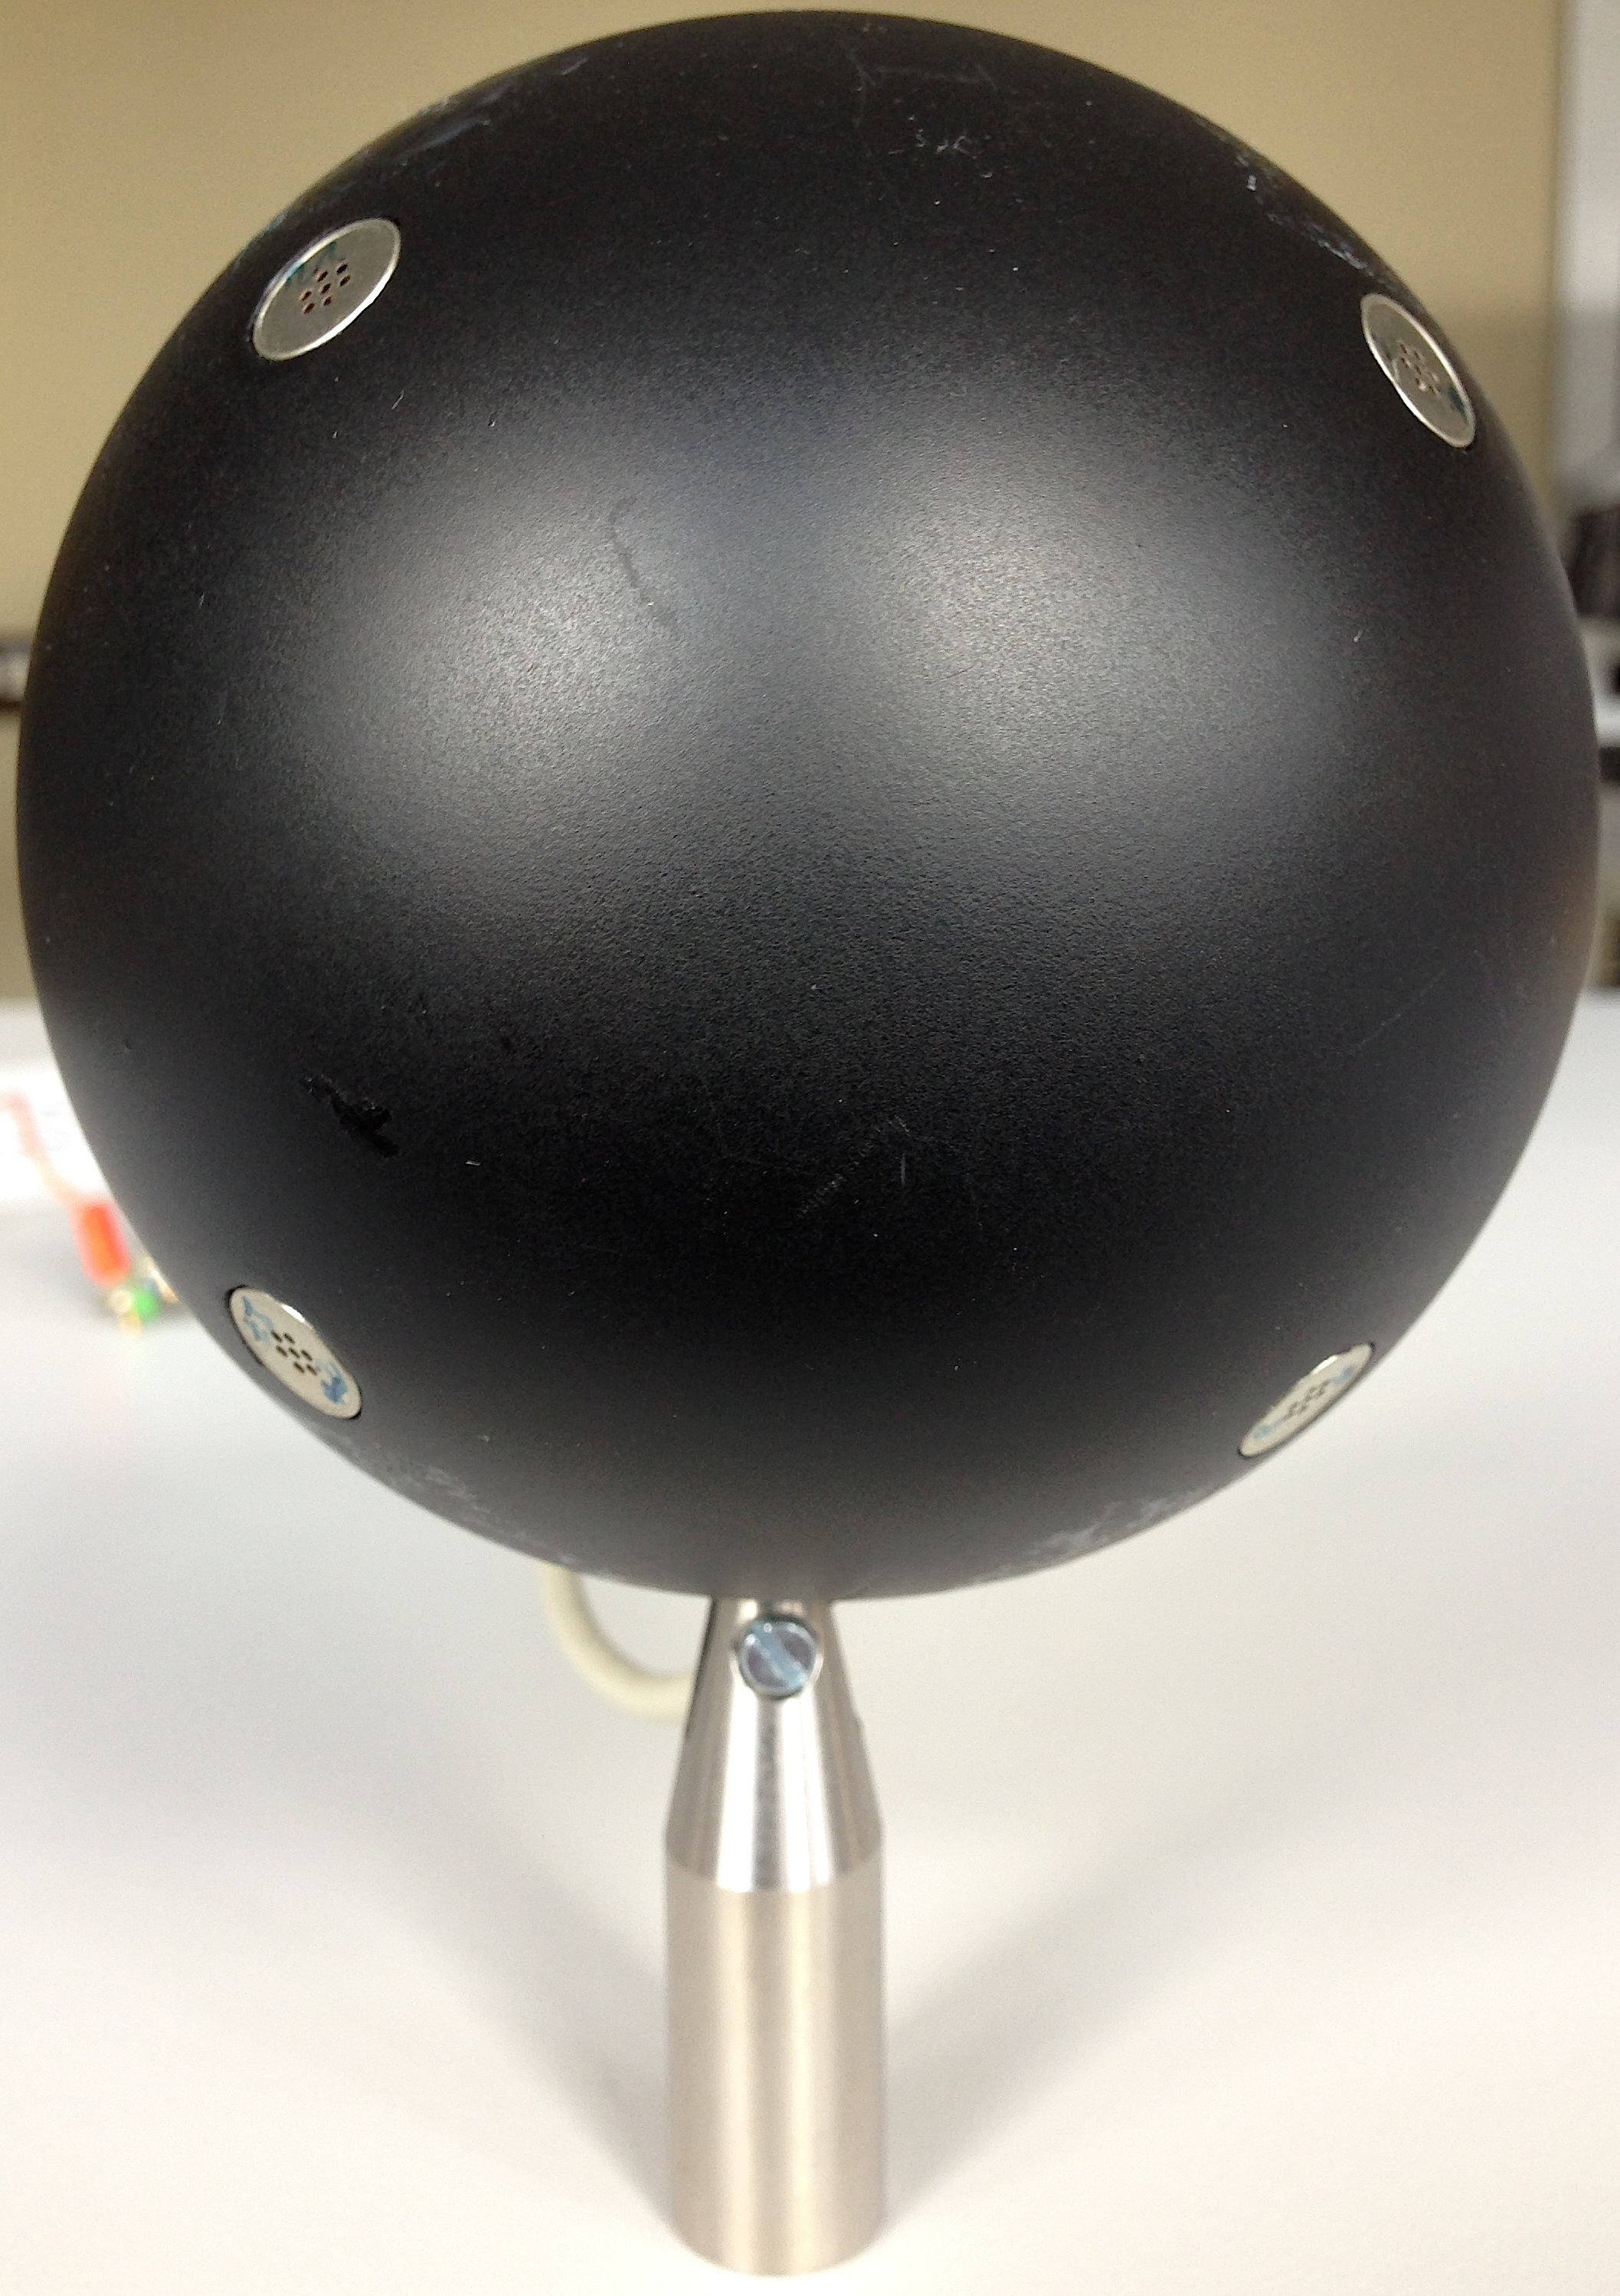
\includegraphics[width=\textwidth]{images/02_Konzeptionierung/Foto_MikrofonArray_Frontansicht}
                \caption{Frontansicht}
                \label{fig:Foto_MikrofonArray_Frontansicht}
        \end{subfigure}
        ~ %add desired spacing between images, e. g. ~, \quad, \qquad etc.
          %(or a blank line to force the subfigure onto a new line)
        \begin{subfigure}[b]{0.35\textwidth}
                \centering
                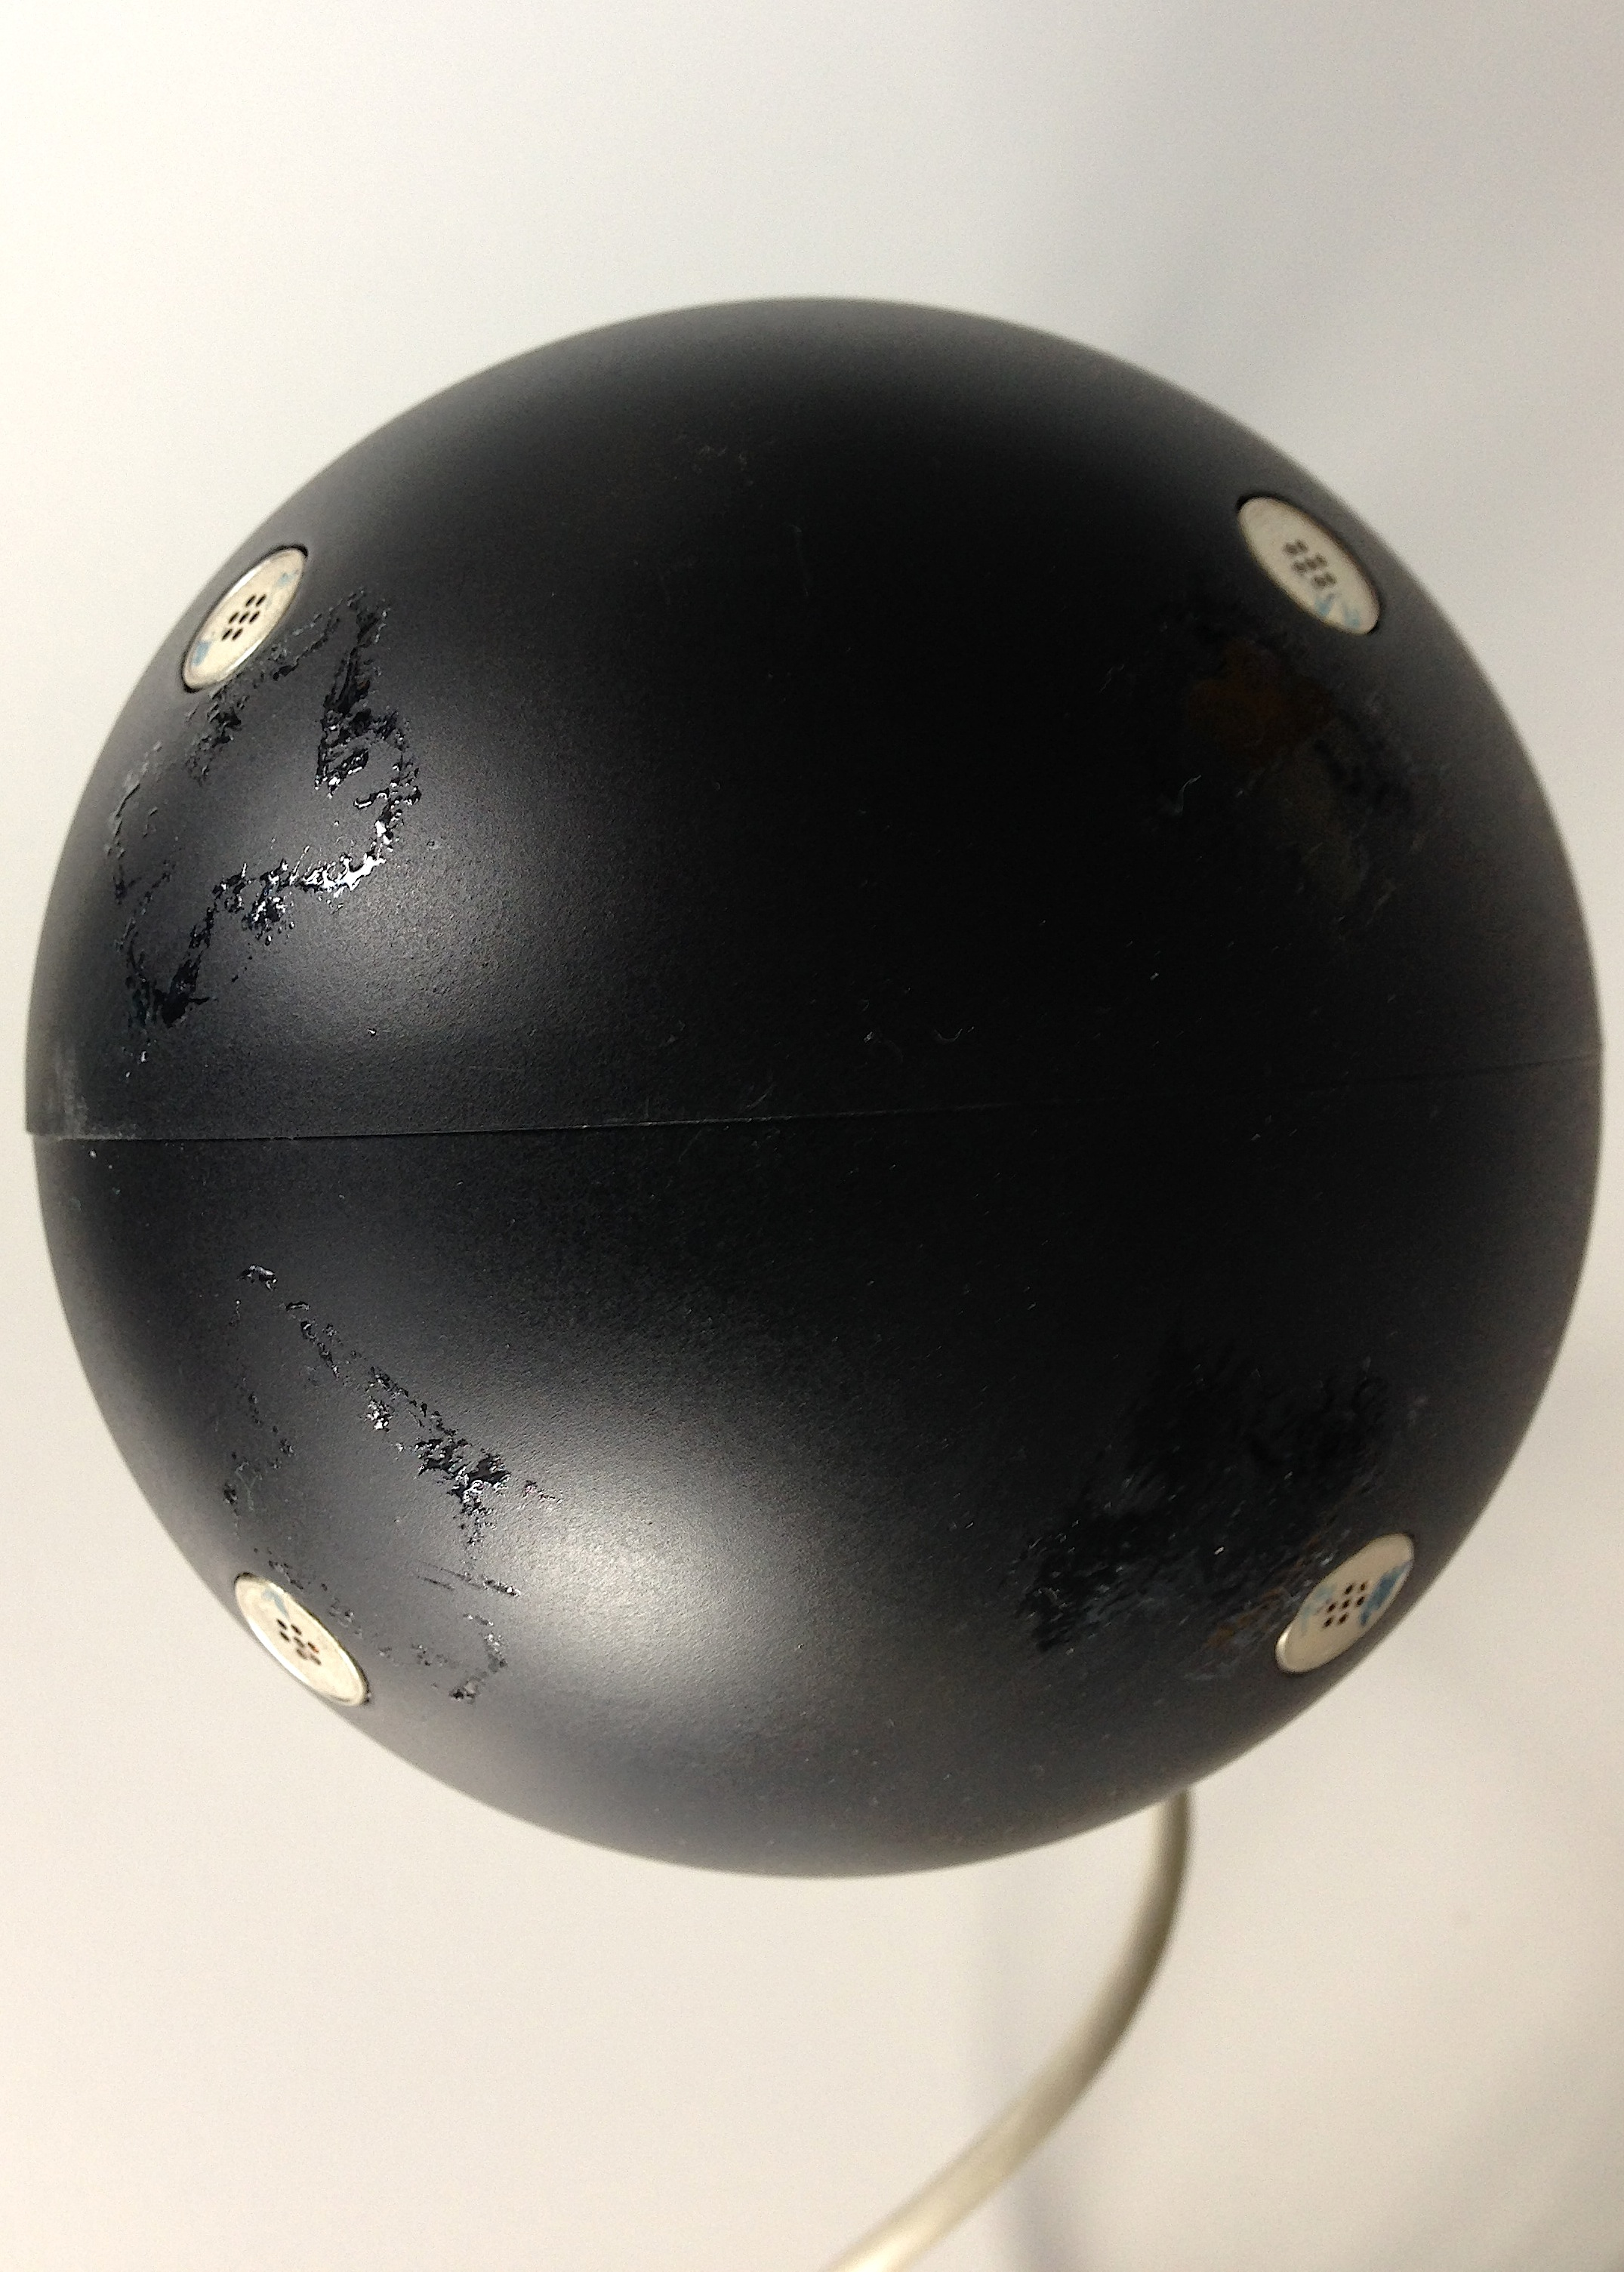
\includegraphics[width=\textwidth]{images/02_Konzeptionierung/Foto_MikrofonArray_Draufsicht}
                \caption{Draufsicht}
                \label{fig:Foto_MikrofonArray_Draufsicht}
        \end{subfigure}
        \caption{kugelförmiges Mikrofonarray}
        \label{fig:Foto_KugelfoermigesMikrofonarray}
\end{figure}
% ----------------------------------------- SUB-FIGURE -----------------------------------




\myFigure{real}                  % Figure tag (missing, real)
         {medium}                 % Size (small,medium,big)
         {h!}             % z.B. htbp
         {Sensoranordnung auf der Kugeloberfläche}                % Figure title
         {SensoranordnungKugeloberflaeche}                % Figure label 
         {02_Konzeptionierung/SensoranordnungKugeloberflaeche}     % Path to real figure








% ****************************************************************************************
\subsection{Untersuchung des kugelförmigen Mikrofonarrays}
\label{sec:UntersuchungKugelArrays}
% ****************************************************************************************
Zur Verifikation des angenommen Schallverhaltens an der schallharten Kugeloberfläche wird im folgenden eine Messung der Sensorlaufzeiten aus einer definierten Richtung durchgeführt und anschließend mit den theoretisch berechneten verglichen. \tab{KugelArray_Laufzeitmessung} zeigt einen tabellarischen Überblick der Messergebnisse. Der Fehler wird hier in Abtastwerten angegeben und bezieht sich auf eine Frequenz von $f_a=48kHz$. 

\begin{table}[h!]
     \center
     \begin{tabular}{cccc}
          \hline
          Sensorpaar & $\tau_{theo} [\mu s ]$ & $\tau_{gemessen} [\mu s ]$ & Fehler [Sample] \\
          \hline \hline
          $m_{13}$    &    272                  &  168                        & 5     \\
          $m_{14}$    &    184                & 168                       & 1  \\
          $m_{17}$    &    384                & 168                       & 11  \\
          $m_{24}$    &    288                  & 168                        & 6  \\
          $m_{28}$    &    384                  & 168                         & 11     \\
          \hline 
     \end{tabular}
  \caption{Laufzeitmessung an kugelförmigem Mikrofonarray bei den Winkeln $\phi=0°$, $\theta = 0°$.}
 \label{tab:KugelArray_Laufzeitmessung}
 \end{table}


Die bei dieser Messung auftretenden Fehler deuten darauf hin, dass sich die Schallwelle nicht wie erwartet geradlinig am Array vorbei bewegen, sondern mit großer Wahrscheinlichkeit an der Kugeloberfläche gebeugt wird. \abb{sim_wave_3000} zeigt eine Simulation (erstellt mit dem \matlab-Skript aus \cite{web_sim_wave}) die das Verhalten eines sinusförmigen Schall-Burst mit einer Frequenz von $f=3kHz$ an einer schallharten Kugel mit dem Radius $r=50mm$ untersucht. Es ist deutlich zu erkennen, dass die Schallwelle erheblich durch das Objekt beeinflusst wird. Eine theoretische Berechnung der Sensorlaufzeiten mit dem in \Sec{subsec:Sensormodell} beschriebenen Modell ist somit nicht möglich. Da das hier zu implementierende System nur mit diskreten Zeiten und somit mit diskreten Winkeln arbeitet können die ermittelten Fehler nicht toleriert werden. Ein Fehler von einem Abtastwert würde einen Fehler von einem Winkelschritt verursachen, wodurch eine zuverlässige Richtungsdetektion unmöglich wäre.


% ----------------------------------------- SUB-FIGURE -----------------------------------
\begin{figure}
        \centering
        \begin{subfigure}[b]{0.48\textwidth}
                \centering
                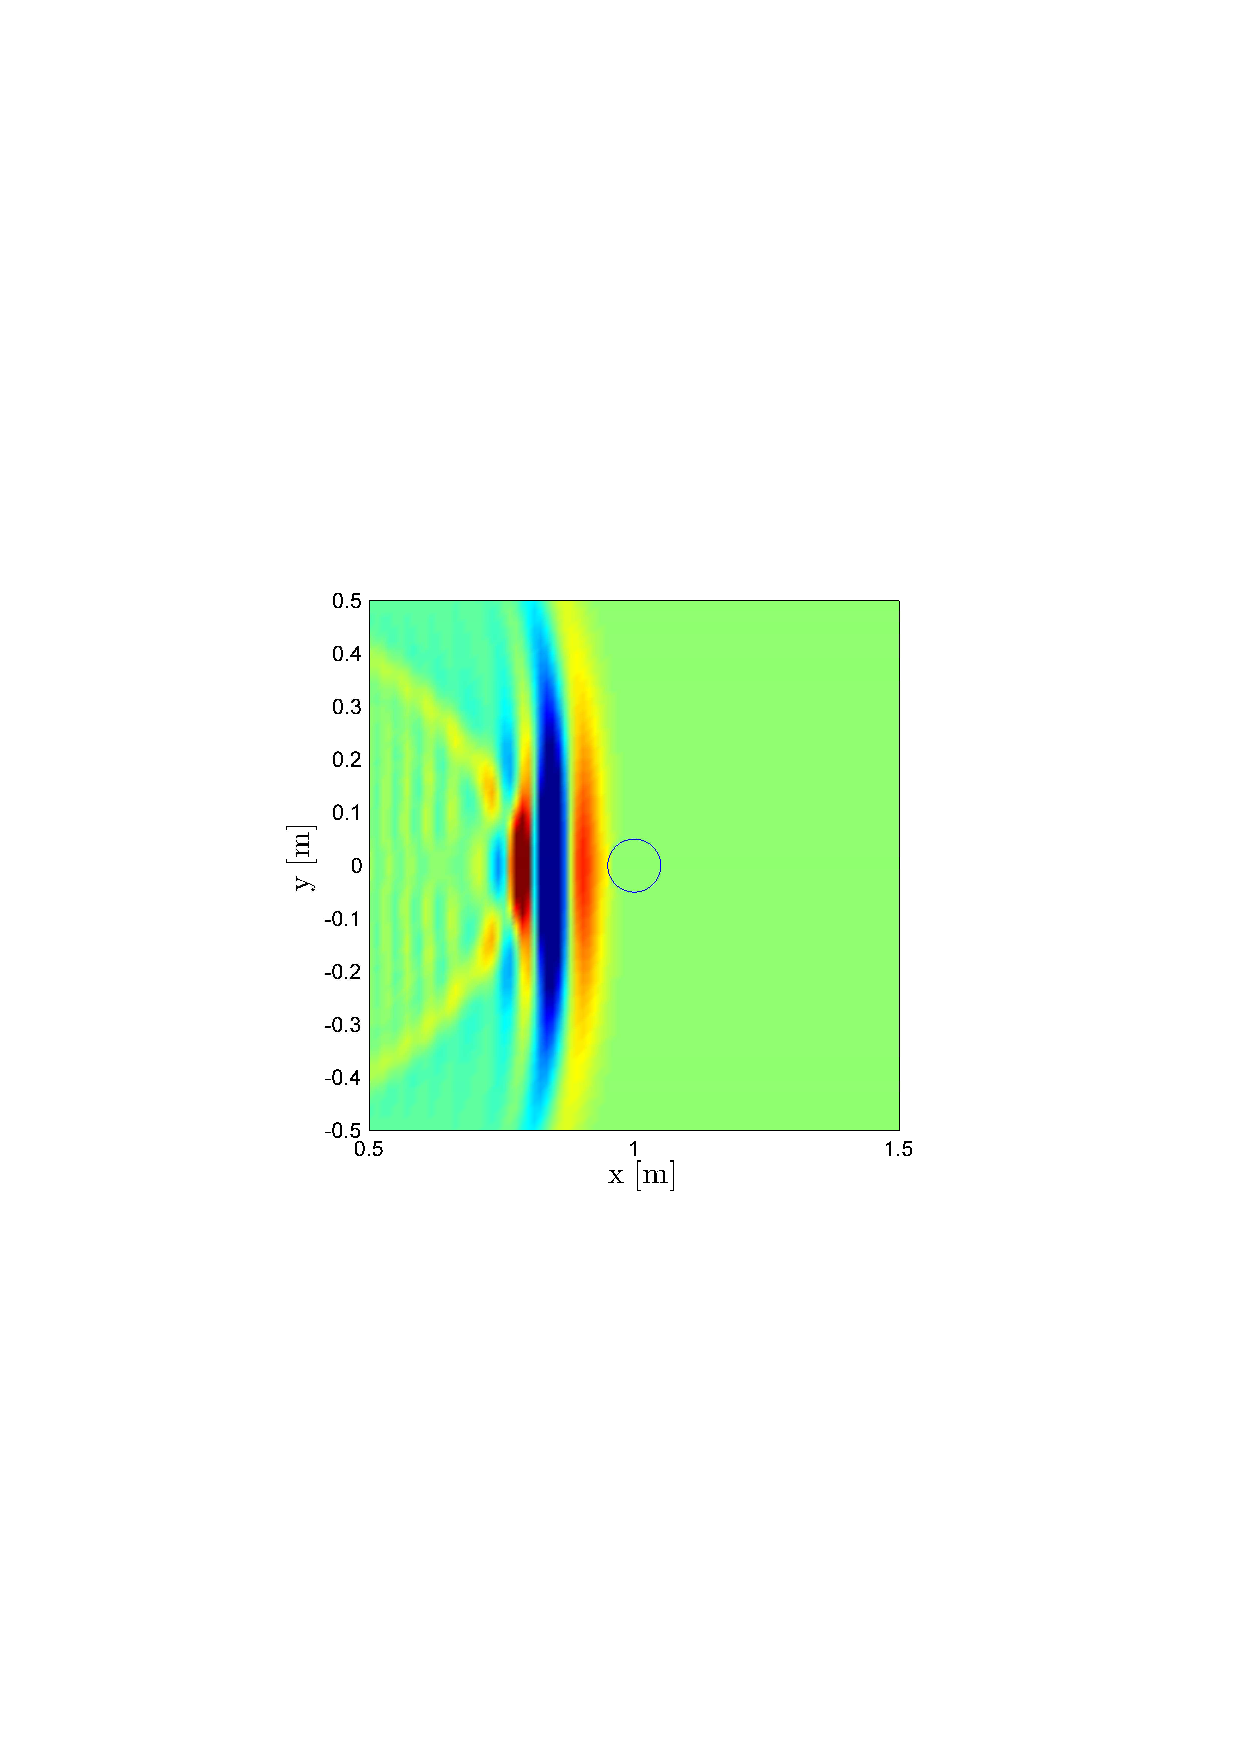
\includegraphics[width=\textwidth]{images/02_Konzeptionierung/sim_wave_3000_1}
                %\caption{Frontansicht}
                %\label{fig:sim_wave_3000_1}
        \end{subfigure}
        ~ %add desired spacing between images, e. g. ~, \quad, \qquad etc.
          %(or a blank line to force the subfigure onto a new line)
        \begin{subfigure}[b]{0.48\textwidth}
                \centering
                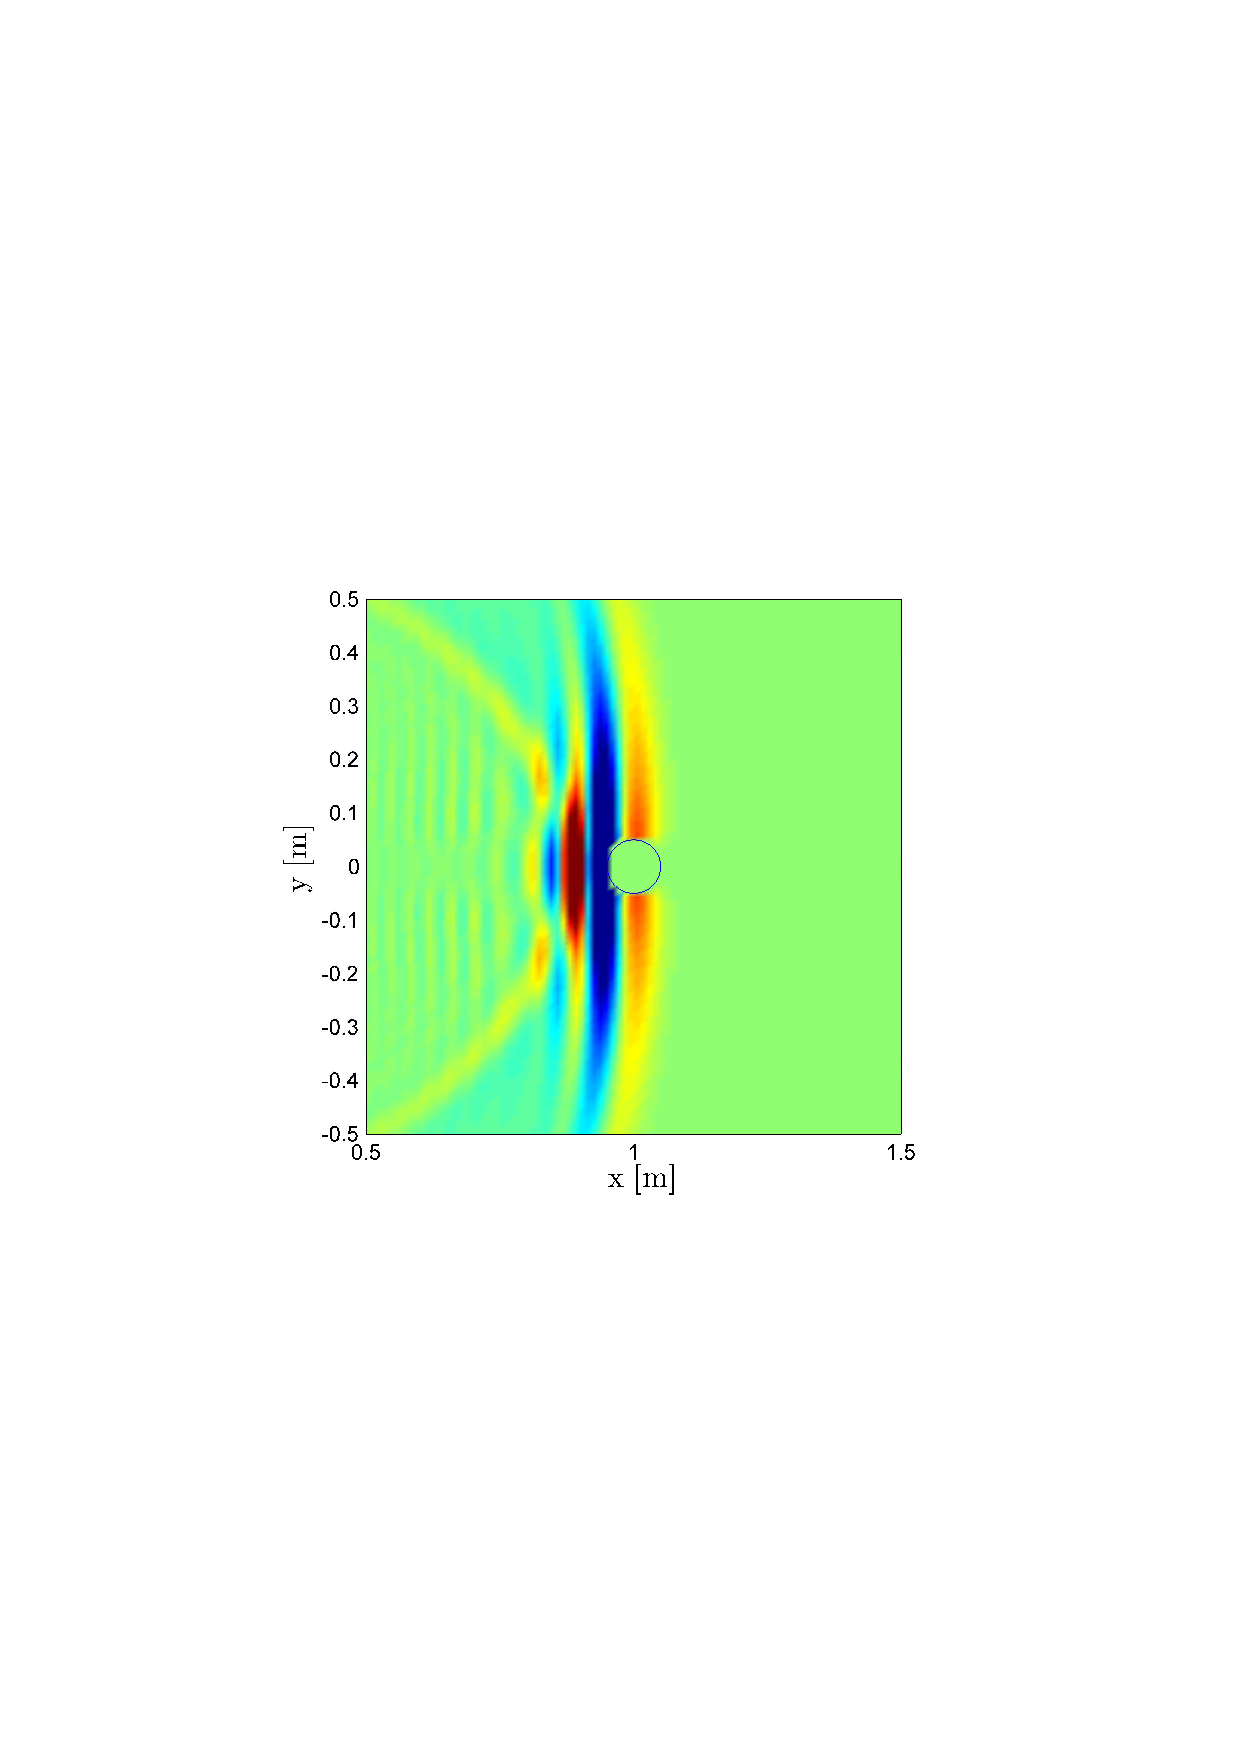
\includegraphics[width=\textwidth]{images/02_Konzeptionierung/sim_wave_3000_2}
                %\caption{Draufsicht}
                %\label{fig:sim_wave_3000_2}
        \end{subfigure}
        ~ %add desired spacing between images, e. g. ~, \quad, \qquad etc.
          %(or a blank line to force the subfigure onto a new line)
        \begin{subfigure}[b]{0.48\textwidth}
                \centering
                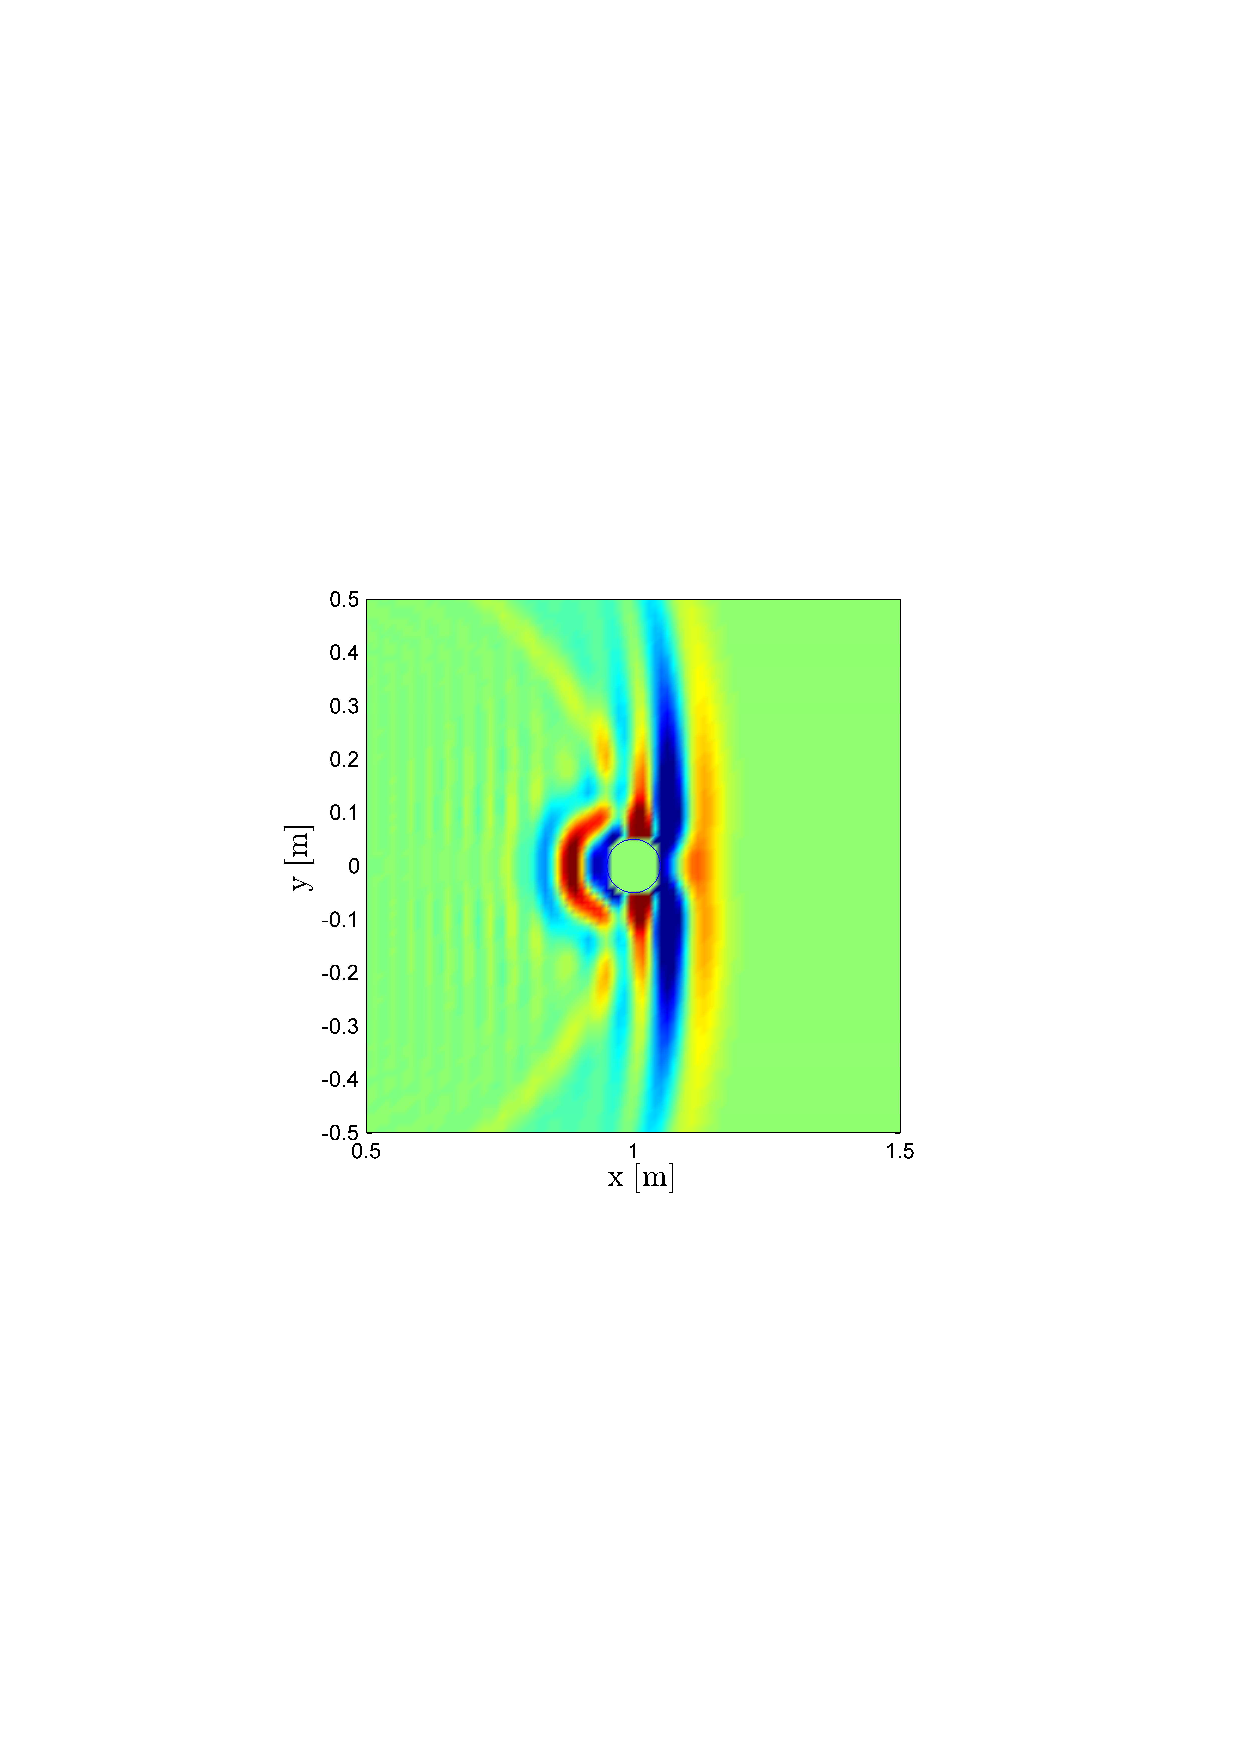
\includegraphics[width=\textwidth]{images/02_Konzeptionierung/sim_wave_3000_3}
                %\caption{Draufsicht}
                %\label{fig:sim_wave_3000_3}
        \end{subfigure}
        ~ %add desired spacing between images, e. g. ~, \quad, \qquad etc.
          %(or a blank line to force the subfigure onto a new line)
        \begin{subfigure}[b]{0.48\textwidth}
                \centering
                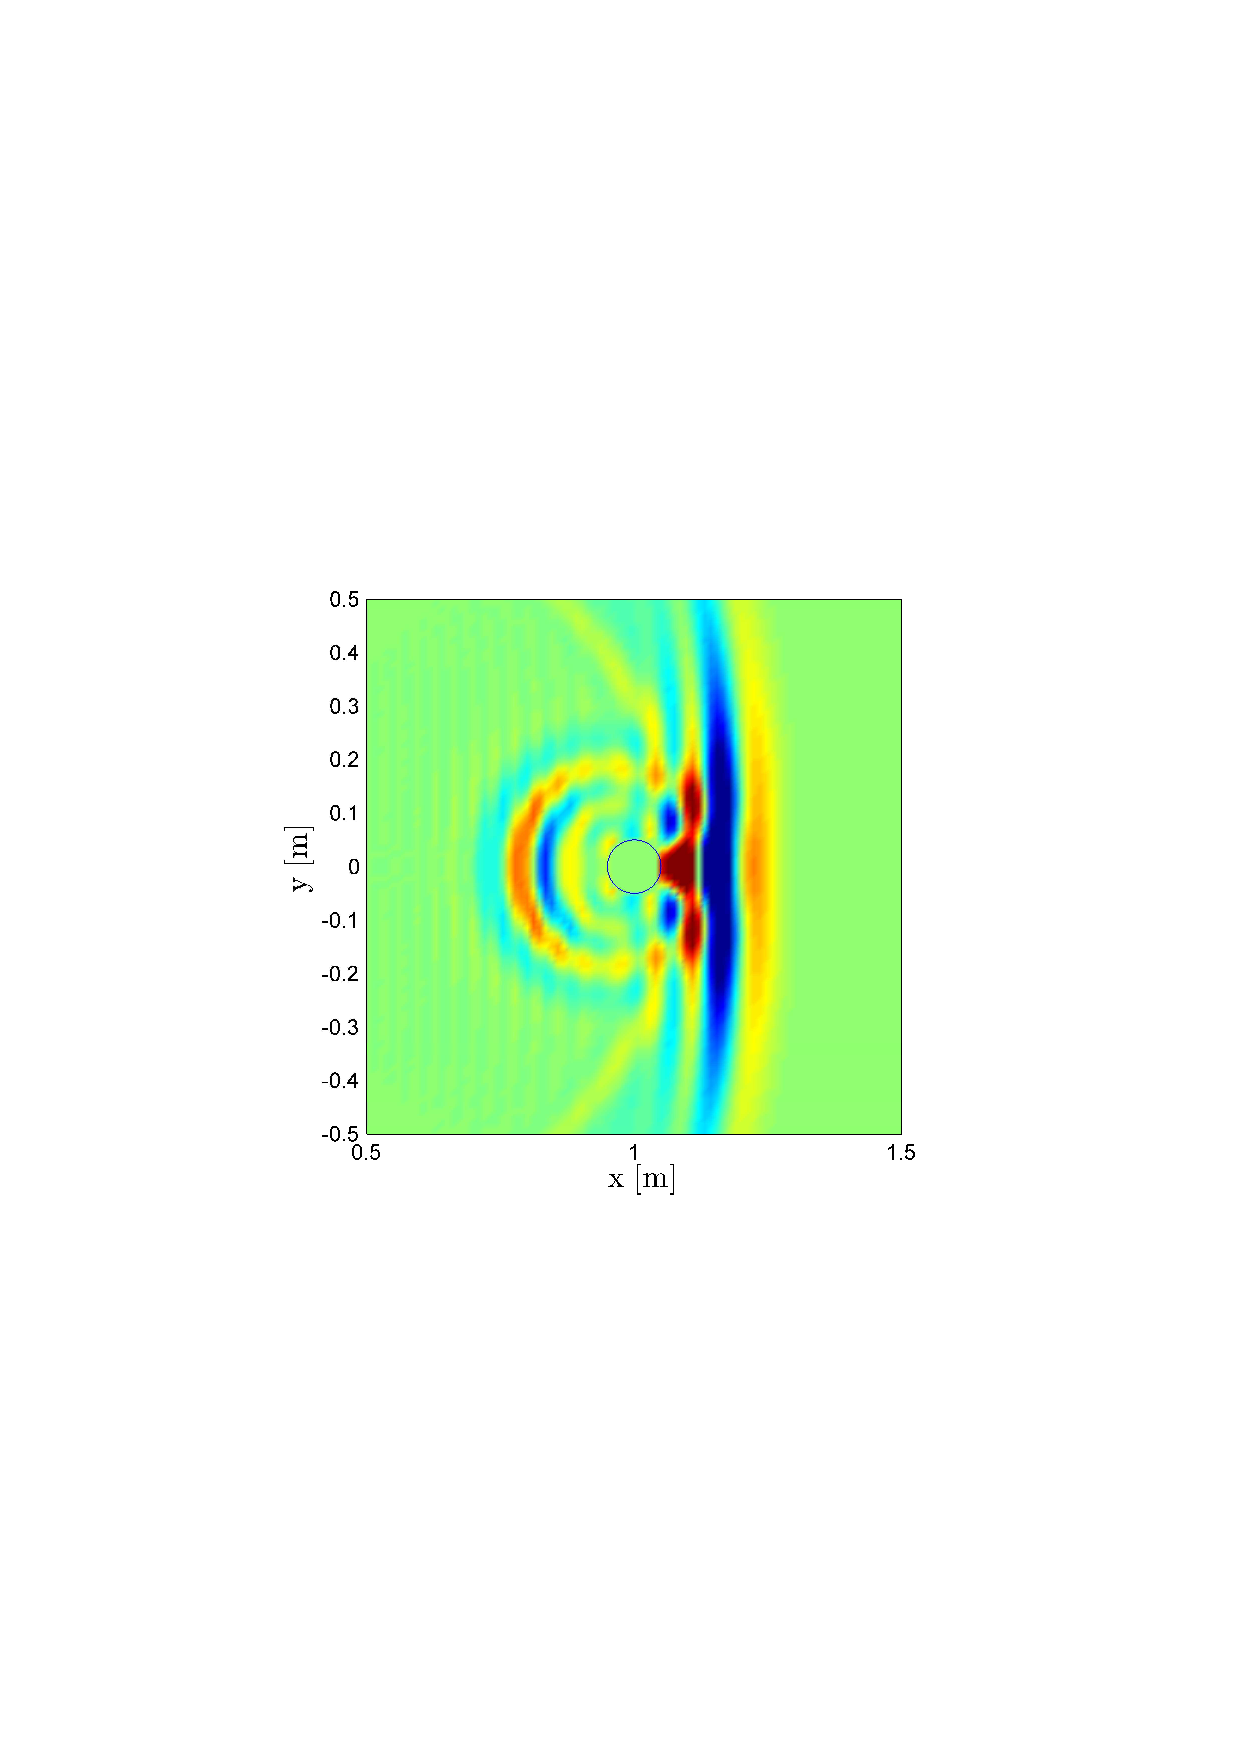
\includegraphics[width=\textwidth]{images/02_Konzeptionierung/sim_wave_3000_4}
                %\caption{Draufsicht}
                %\label{fig:sim_wave_3000_4}
        \end{subfigure}
        \caption{Schallverhalten an schallharter Kugel ($r=50mm$) mit einer Schallwelle der Wellenlänge $\lambda = 114mm$ und einer Frequenz von $f=3kHz$.}
        \label{fig:sim_wave_3000}
\end{figure}
% ----------------------------------------- SUB-FIGURE -----------------------------------






% ****************************************************************************************
\subsection{Mikrofonarray Neudesign/Konstruktion}
\label{subsec:MikrofonarrayNeudesign}
% ****************************************************************************************
Auf Basis der unter \Sec{sec:UntersuchungKugelArrays} gewonnen Erkenntnisse sowie der im \Sec{subsec:Sensormodell} erläuterten Zusammenhänge erfolgt in diesem Abschnitt eine Neukonstruktion des kugelförmigen Mikrofonarrays.

Um eine zuverlässige Aussage über die Schallausbreitung treffen zu können, muss der Körper des Mikrofonarray auf seine minimal nötigen Elemente reduziert werden. \abb{Prinzip_Konstruktion_NewArray} zeigt die prinzipielle Konstruktionsidee. Alle schallharten Bestandteile die einen unvorhersehbaren Einfluss auf die Schallausbreitung haben könnten, wurden entfernt, so dass der Körper nun lediglich aus dünnen Drähten besteht. Da sich die Mikrofonkapseln im Vergleich zur Kugel exakt an den selben Stellen befinden, kann dieses Array als Acht-Punkte-Approximation der Kugelgeometrie betrachtet werden.

Zur Prüfung des Schallverhaltens wurde der in \abb{Prototyp_Array} illustrierte Prototyp hergestellt. Die Drahtkonstruktion besteht dabei aus $1mm$ dicken Kupferdrähten, die an den Enden fest mit Lötzinn verbunden sind. Die Mikrofonkapseln wurden mit Hilfe von transparentem Kunststoff (Plexiglas) sowie Heißklebstoff in der oben beschriebenen Abstandsmetrik angeordnet. Die Kapseln selber wurden dabei im Hinblick auf eine spätere Mikrofonkonstruktion aus Pertinax\footnote{Phenolharz mit Papierfasern (sog. Hartpapier)}(inkl. einer dünnen Oberflächenschicht aus Kupfer) lediglich mit Klebeband fixiert.


\myFigure{real}                  % Figure tag (missing, real)
         {medium}                 % Size (small,medium,big)
         {h!}             % z.B. htbp
         {Prinzip der Mikrofonkonstruktion}                % Figure title
         {Prinzip_Konstruktion_NewArray}                % Figure label 
         {02_Konzeptionierung/Prinzip_Konstruktion_NewArray}     % Path to real figure



\myFigure{real}                  % Figure tag (missing, real)
         {medium}                 % Size (small,medium,big)
         {h!}             % z.B. htbp
         {Prototyp des würfelförmigen Mikrofonarrays}                % Figure title
         {Prototyp_Array}                % Figure label 
         {02_Konzeptionierung/Prototyp_Array}     % Path to real figure



% ****************************************************************************************
\subsubsection{Laufzeitmessung am Prototyp}
% ****************************************************************************************
\tab{Prototyp_NewArray_Laufzeitmessung} zeigt die Ergebnisse von zwei Laufzeitmessungen aus unterschiedlichen Schalleinfallsrichtungen. Gemessen wurden immer die Laufzeitdifferenzen zum Referenzmikrofon $M_1$. Zur Verifikation der Geometrie wurde das Array mit einem durch einen Lautsprecher abgestrahlten Rechteckimpuls angeregt. Die dazu benötigten theoretischen Laufzeitdifferenzen wurden mit der in \Eq{DOA_winkel} eingeführten Mikrofonfunktion $f_n(\phi, \theta)$ errechnet. Die Differenz zwischen theoretischem und gemessenem Wert wird als Anzahl von Abtastwerten mit einer Frequenz von $f_a = 48kHz$ angegeben. Die Messergebnisse weichen nur leicht von den theoretisch berechneten ab, so dass sich die Arraykonstruktion aus dünnen Drähten als geeignet erweist.

Da die Konstruktion, bedingt durch die dünnen Kupferdrähte, mechanisch sehr instabil ist und die Mikrofonkapseln im Vergleich zur Kugel nicht exakt gleich angeordnet sind, wird im Folgenden eine Neukonstruktion des Array vorgestellt.


\begin{table}[]
     \center
     \begin{tabular}{cccc}
          \hline
          Sensorpaar & $\tau_{theo} [\mu s ]$ & $\tau_{gemessen} [\mu s ]$ & Fehler [Sample] \\
          \hline \hline
          $\phi = 0°, \theta = 0°$ \\
          \hline
          $m_{12}$    &    0                  &  0                        & 0        \\
          $m_{13}$    &    168                & 165                       & 0,14        \\
          $m_{14}$    &    168                & 162                       & 0,28        \\
          $m_{15}$    &    0                  & 12                        & 0,57       \\
          $m_{16}$    &    0                  & 0                         & 0        \\
          $m_{17}$    &    168                & 155                       & 0,62    \\
          $m_{18}$    &    168                & 150                       & 0,84    \\
          \hline
            %          &                       &            Mittelwert     & 0,19    \\
          \hline
          $\phi = 45°, \theta = 45°$ \\
          \hline
          $m_{12}$    &   -84                 &  -90                      & 0,28        \\
          $m_{13}$    &    0                  & 0                         & 0        \\
          $m_{14}$    &    84                 & 84                        & 0        \\
          $m_{15}$    &    119                & 112                       & 0,33       \\
          $m_{16}$    &    34                 & 50                        & -0,76        \\
          $m_{17}$    &    119                & 130                       & -0,52    \\
          $m_{18}$    &    203                & 190                       & 0,62    \\
          %\hline
          %            &                       &            Mittelwert     & 0    \\
          \hline 
     \end{tabular}
  \caption{Laufzeitmessung aus zwei unterschiedlichen Schalleinfallsrichtungen}
 \label{tab:Prototyp_NewArray_Laufzeitmessung}
 \end{table}
 

%\todo[inline]{Hier eine Grafik mit Matlab ploten und für jede Richting (also ein paar Winkelpaare) mit der Formel aus von Benesty einfügen um die Genauigkeit darzustelln K=Anzahl der gemessenen Mikrofonpaare $f_{Stabw}(\phi, \theta) = \sqrt{\frac{1}{K-1} \sum_{i=1}^{K} \left[ f_{theory}(\phi, \theta) - f_i(\phi, \theta) \right]^2}$}



% Bilder zur Laufzeitmessung
% ----------------------------------------- SUB-FIGURE -----------------------------------
%\begin{figure}
%        \centering
%        \begin{subfigure}[b]{0.48\textwidth}
%                \centering
%                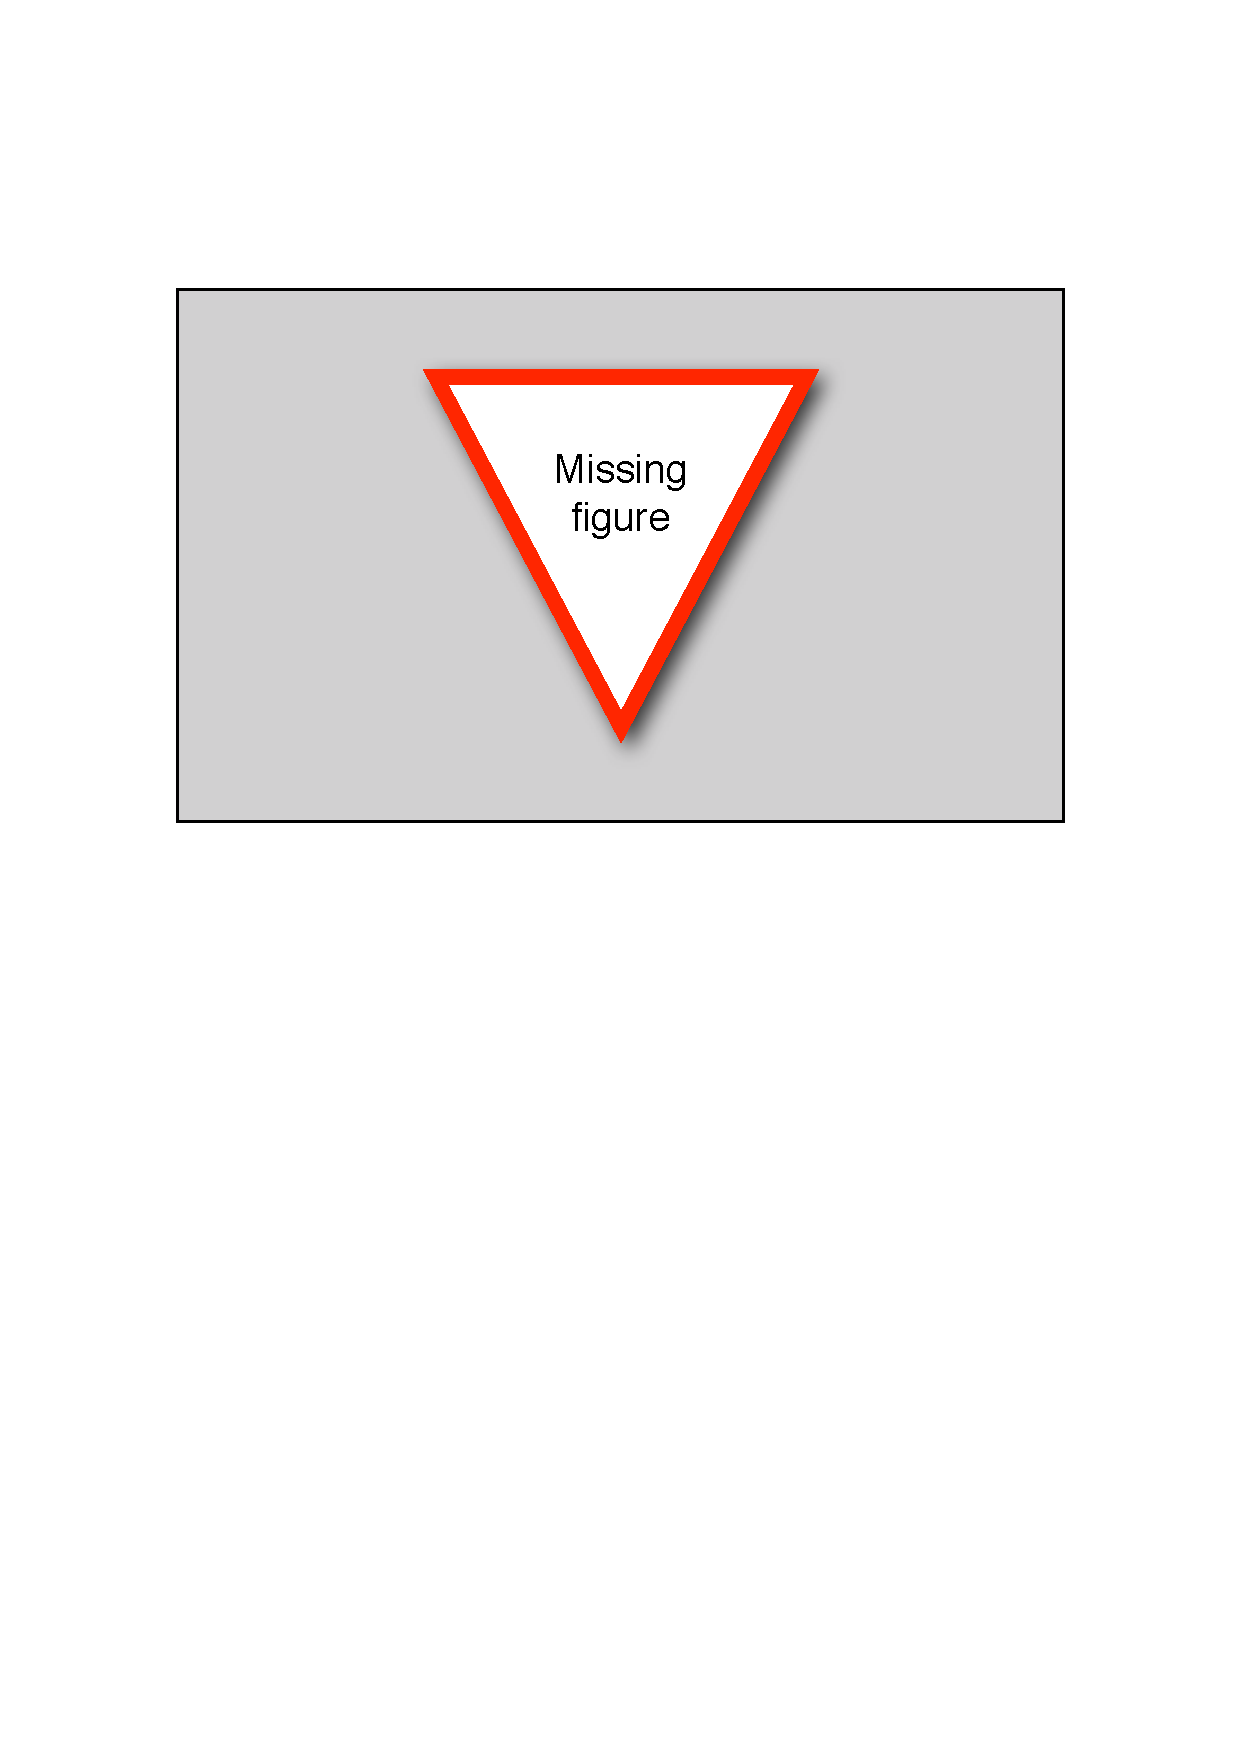
\includegraphics[width=\textwidth]{images/MissingFigure}
%                \caption{$\phi=0°, \theta=0°$}
%                \label{fig:Richtung1}
%        \end{subfigure}
%        ~ %add desired spacing between images, e. g. ~, \quad, \qquad etc.
%          %(or a blank line to force the subfigure onto a new line)
%        \begin{subfigure}[b]{0.48\textwidth}
%                \centering
%                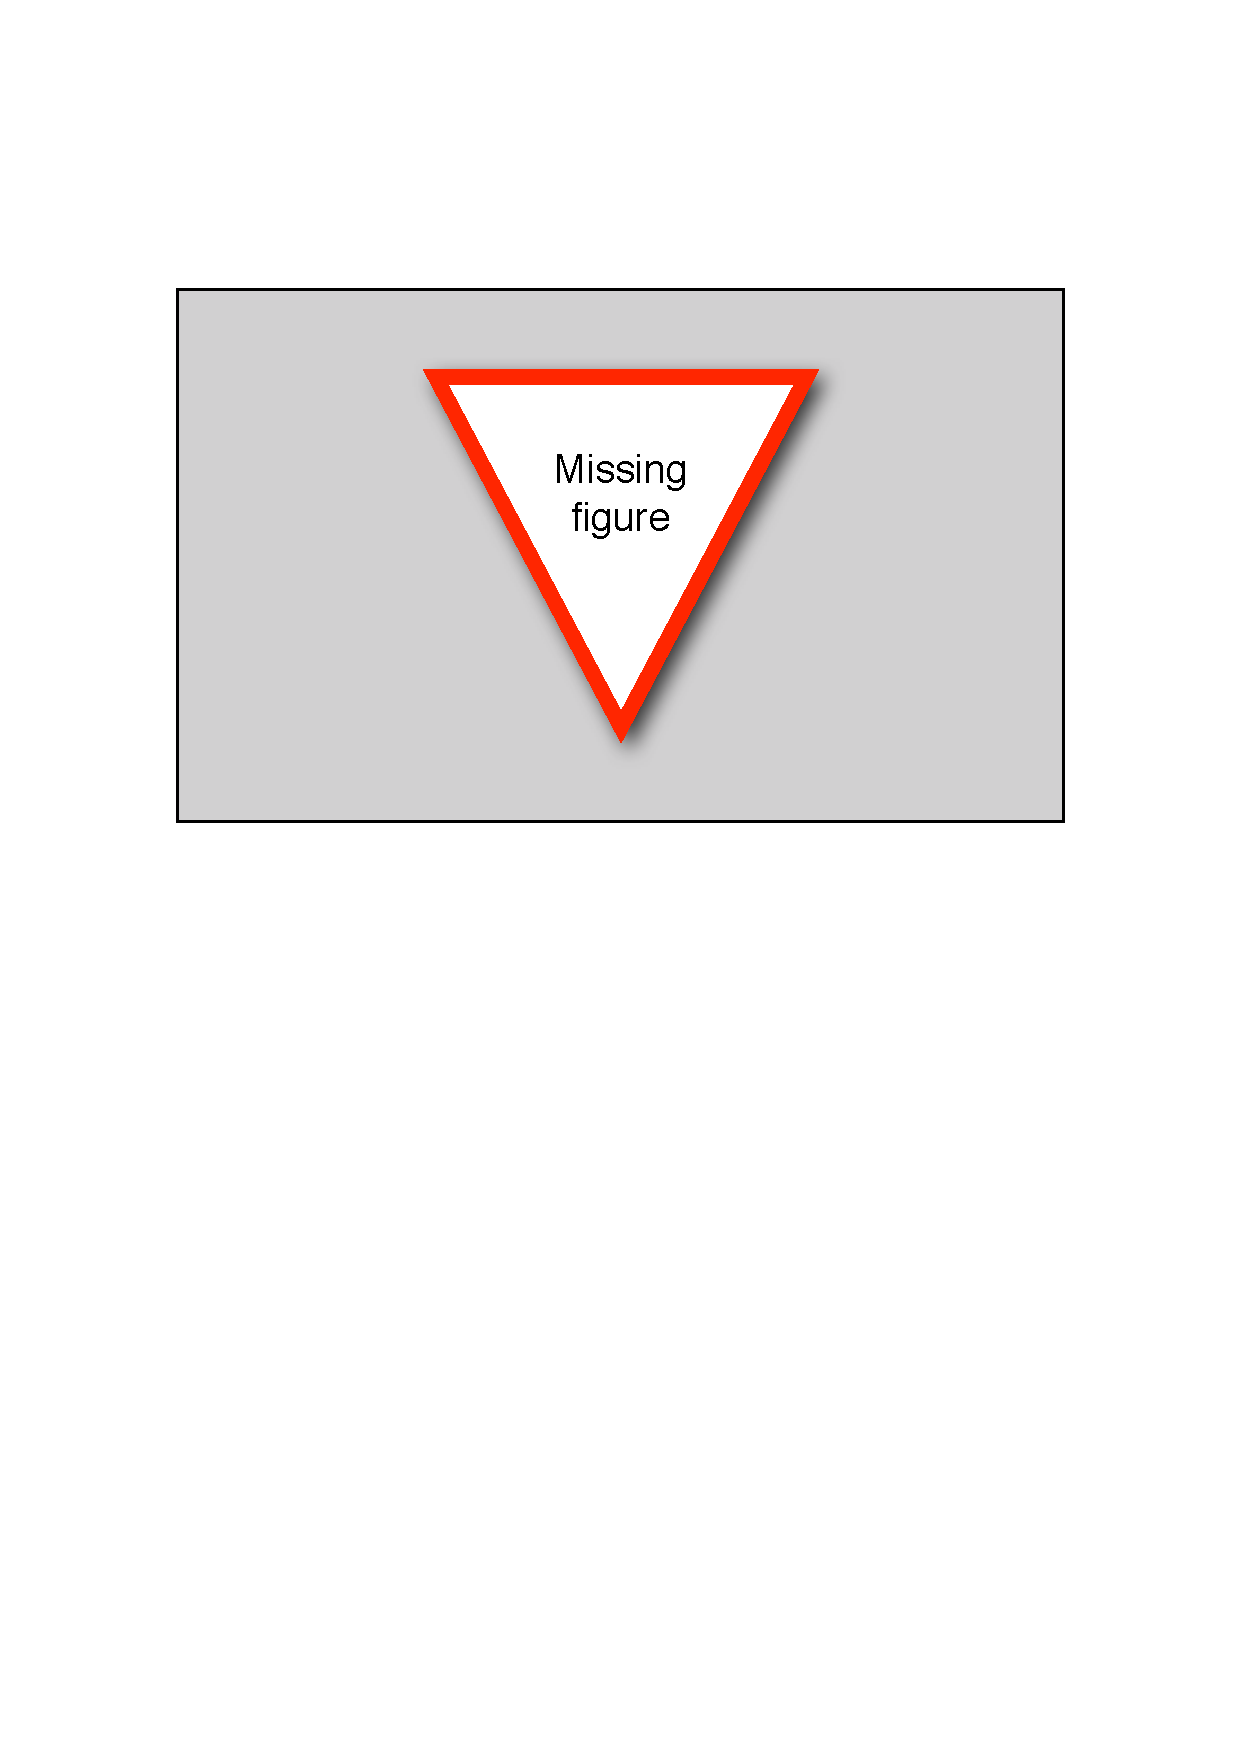
\includegraphics[width=\textwidth]{images/MissingFigure}
%                \caption{$\phi=0°, \theta=45°$}
%                \label{fig:Richtung2}
%        \end{subfigure}
%        ~
%        \begin{subfigure}[b]{0.48\textwidth}
%                \centering
%                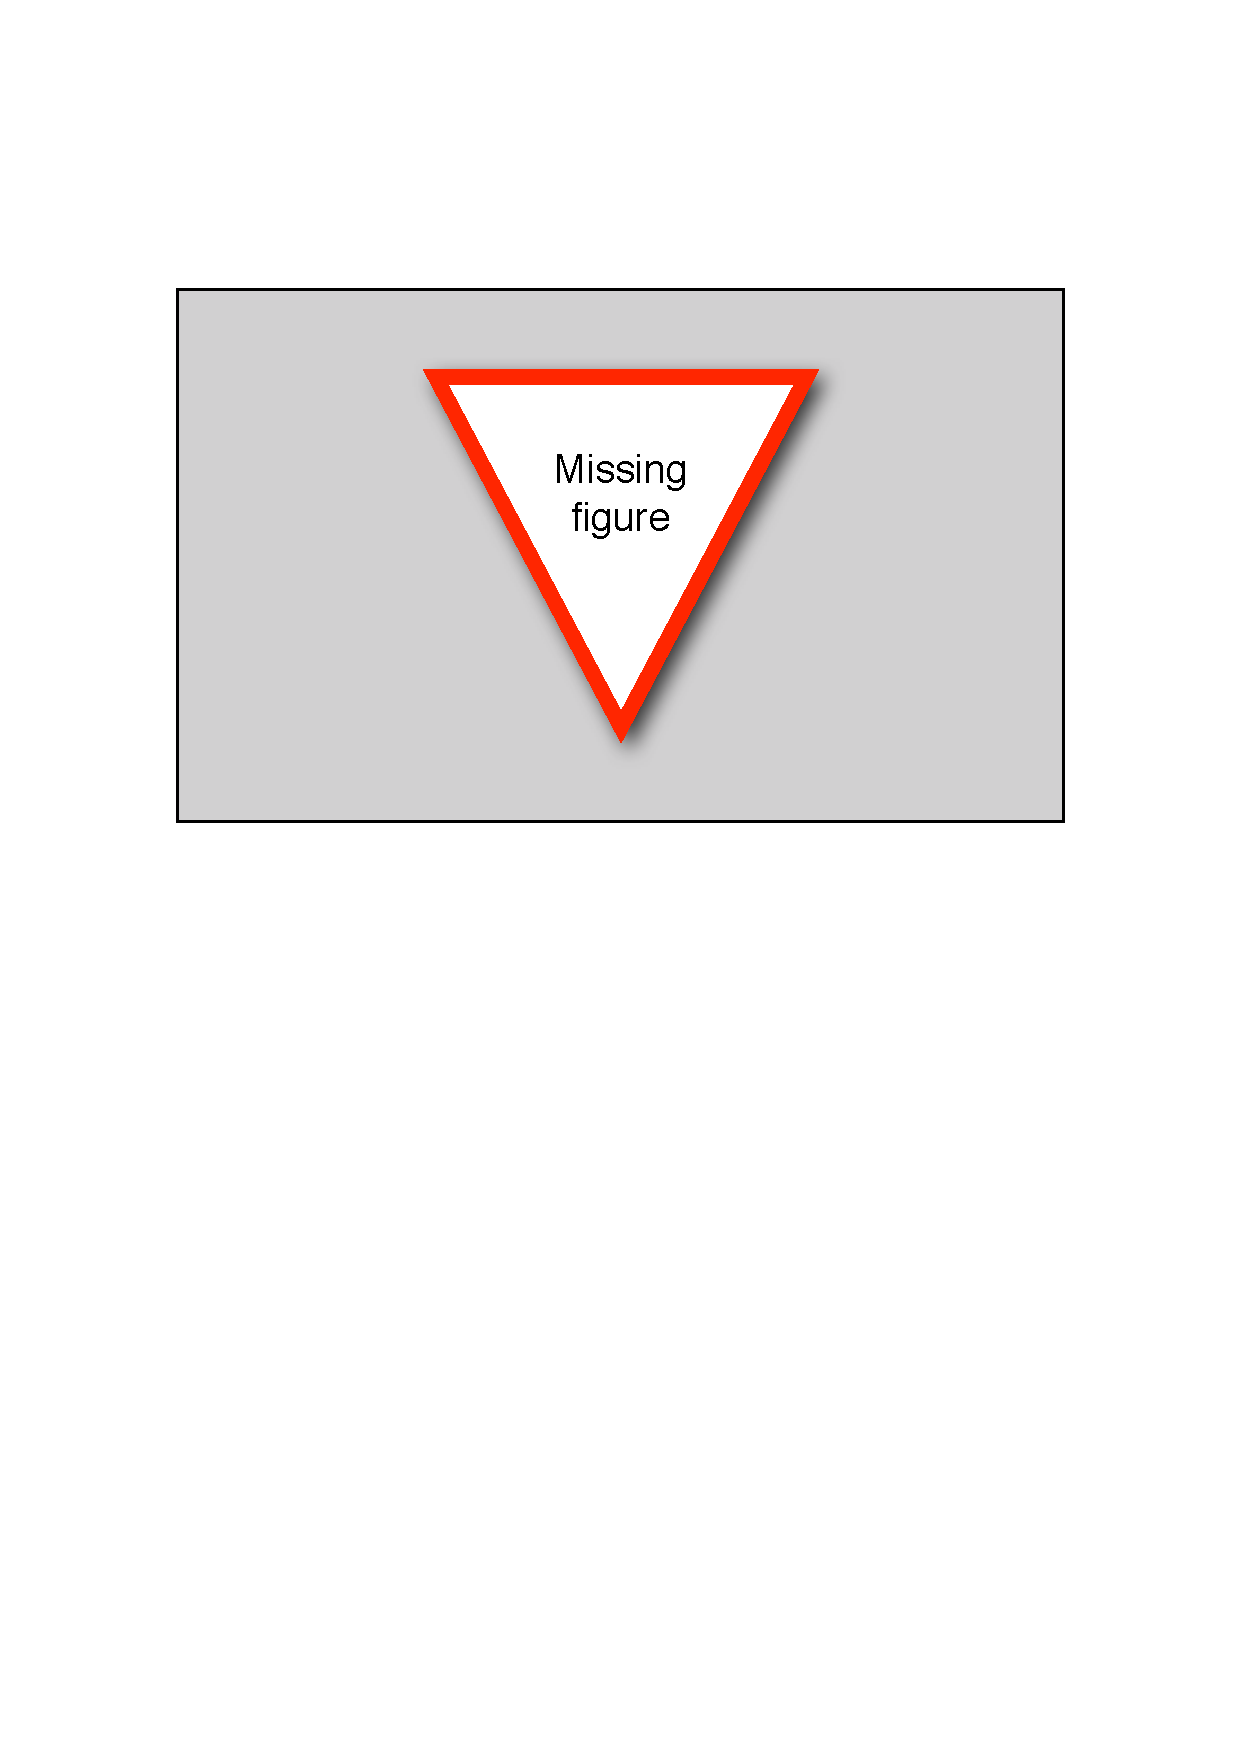
\includegraphics[width=\textwidth]{images/MissingFigure}
%                \caption{$\phi=45°, \theta=0°$}
%                \label{fig:Richtung3}
%        \end{subfigure}
%        ~
%        \begin{subfigure}[b]{0.48\textwidth}
%                \centering
%                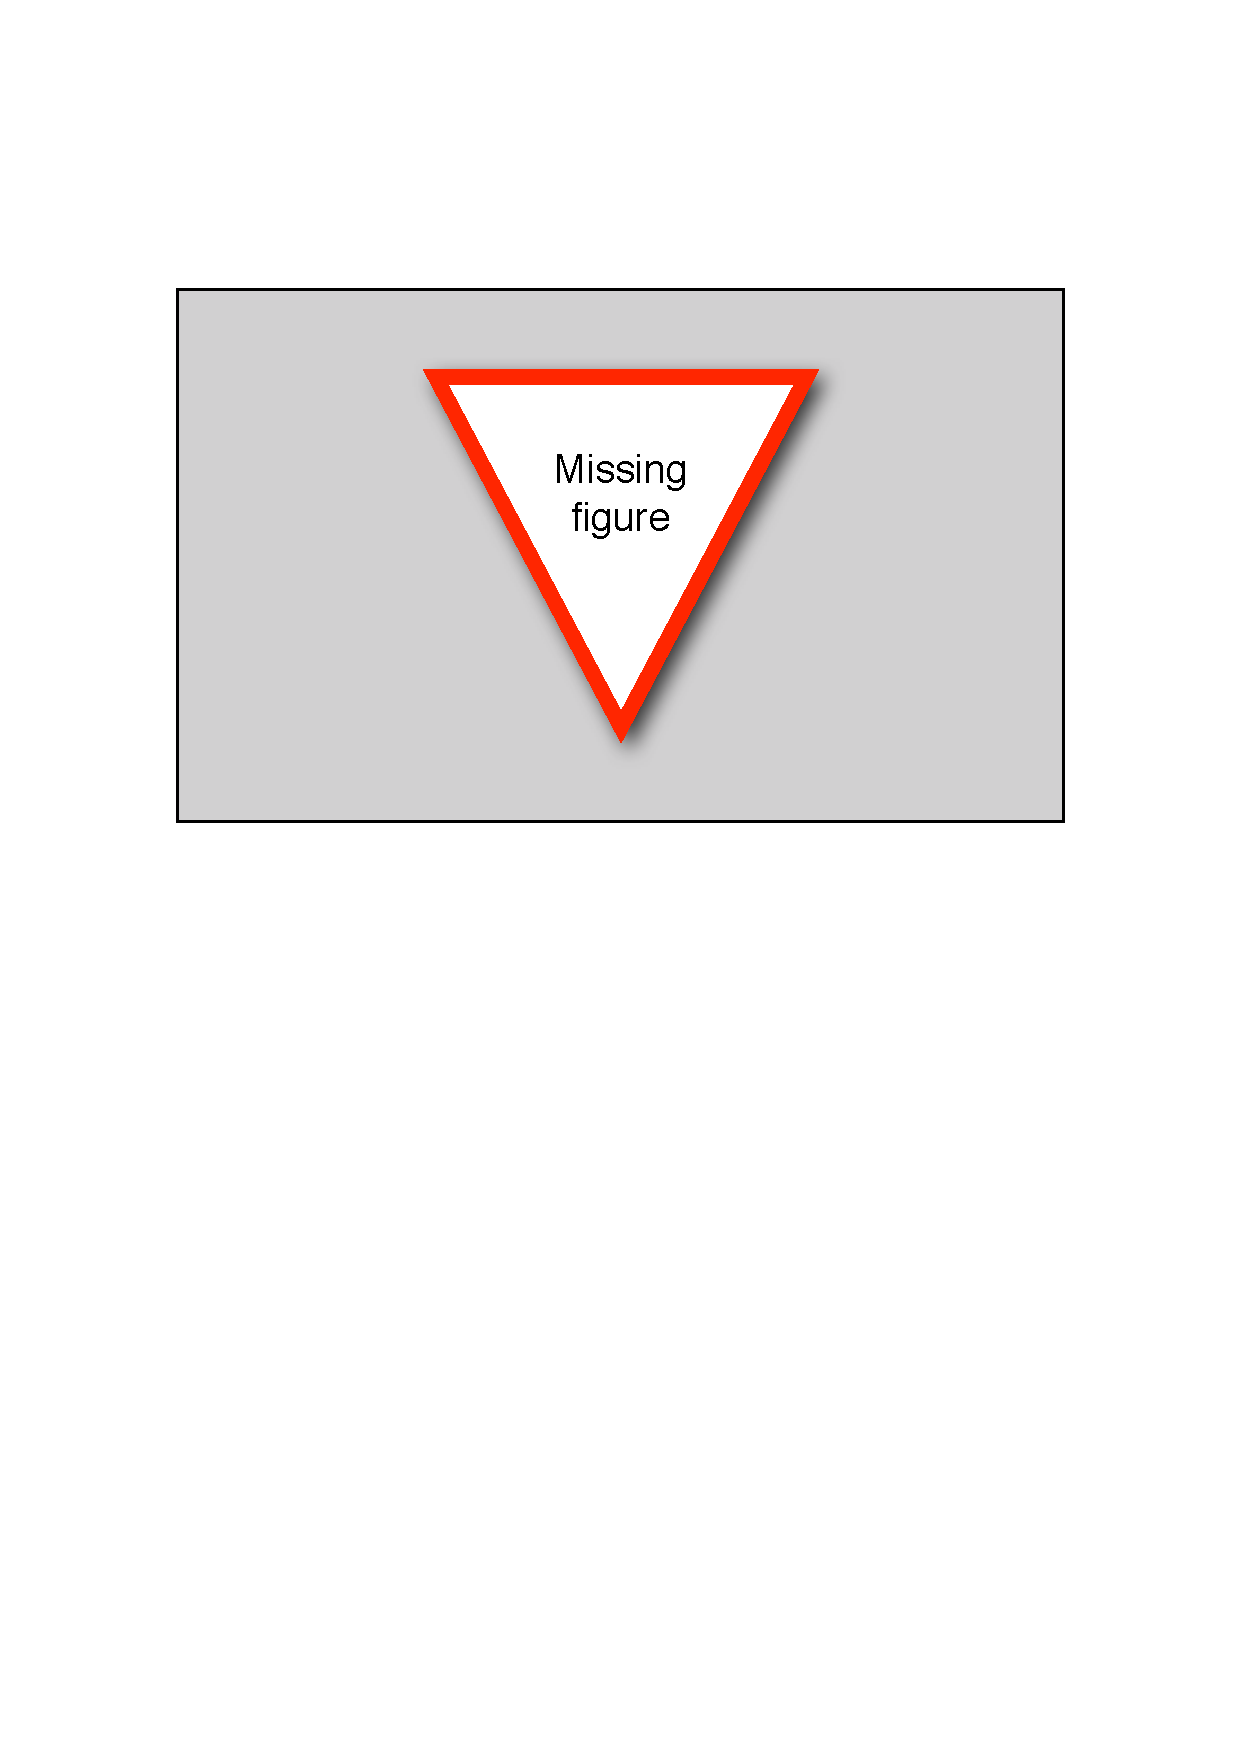
\includegraphics[width=\textwidth]{images/MissingFigure}
%                \caption{$\phi=45°, \theta=45°$}
%                \label{fig:Richtung4}
%        \end{subfigure}
%        \stepcounter{missingFigureCount}
%        \caption{\textbf{\textcolor{red}{Missing Figure \themissingFigureCount}} - Laufzeitmessung am Array-Prototyp}
%        \label{fig:Prototyp_NewArray_Laufzeitmessung}
%\end{figure}
% ----------------------------------------- SUB-FIGURE -----------------------------------


















% ****************************************************************************************
\subsubsection{Äquidistante Arraykonstruktion}
% ****************************************************************************************
Auf Basis der Array-Prototyp Idee wird in diesem Abschnitt ein Array entwickelt, das über eine ausreichend hohe Genauigkeit sowie mechanische Festigkeit verfügt.

Zur Bestimmung der minimal nötigen Herstellungsgenauigkeit wird die Eigenschaft des hier vorliegenden diskreten Systems genutzt. Auf Grund der Zeitdiskretisierung können nur Laufzeitdifferenzen gemessen werden, die ein Vielfaches der Abtastperiode $T_a$ betragen. Die Strecke $d_{T_a}$, die vom Schall innerhalb einer Abtastperiode zurückgelegt wird, ergibt sich durch

\begin{equation}
    d_{T_a} = c \cdot T_a = \frac{c}{f_a}
\end{equation}

\tab{Toleranz_Abtastfrequenz} zeigt unterschiedliche Toleranzbereiche bei den im Audiobereich gängigen Abtastraten. Um einen Messfehler der Laufzeitdifferenz zu vermeiden, muss der entsprechende Toleranzbereich eingehalten werden.


\begin{table}[h]
     \center
     \begin{tabular}{ccc}
     \hline
          Abtastfrequenz [kHz] & $d_{T_a}$ [mm] & Toleranz [mm] \\
           \hline \hline
          8                    & 42,8           & $\pm 21,4$\\
          16                   & 21,4           & $\pm 10,7$\\
          24                   & 14,3           & $\pm 7,1$\\
          48                   & 7,1            & $\pm 3,5$\\
          96                   & 3,5            & $\pm 1,8$\\
         \hline
     \end{tabular}
  \caption{Toleranzbereich bei unterschiedlichen Abtastfrequenzen}
 \label{tab:Toleranz_Abtastfrequenz}
 \end{table}


Als grundsätzliche Konstruktionsidee wird hier ein Steckmechanismus eingesetzt. Die Einzelteile können so aus einem flachen Werkstoff (\zB einer Blechtafel oder Pertinaxplatten) ausgeschnitten werden. Fertigungsprozesse solcher Art sind aufwandsarm da die Einzelteile mit einem CNC\footnote{Computerized Numerical Control}-Laser oder einer CNC-Wasserschneidemaschine aus großen Werkstofftafeln ausgearbeitet werden können. Auf Grund der hohen Schneidegeschwindigkeit moderner Werkzeugmaschinen und der geringen Einricht -und Spannzeit kann solch eine Konstruktion bereits in geringer Stückzahl kostengünstig hergestellt werden.

Zur Befestigung der einzelnen Teile miteinander werden, wie in \abb{3D_Konstruktion_Steckmechanismus} dargestellt, entsprechende Ausschnitte eingearbeitet an denen diese dann zusammengesteckt werden. Um eine ausreichend hohe Festigkeit der Steckverbindung zu gewährleisten, werden diese Ausschnitte entsprechend einer Übergangspassung angefertigt. \abb{3D_Konstruktion_Geundkoerper} zeigt die beiden X-förmigen Grundelemente der Konstruktion. Diese bilden nach dem Zusammenstecken die vier durch das Zentrum laufenden Streben der in \abb{Prinzip_Konstruktion_NewArray} gezeigten Prinzipskizze.

Zur Befestigung der empfindlichen Mikrofonkapseln wird ebenfalls ein Steckmechanismus entworfen. Wie in \abb{3D_Konstruktion_Mikrofonhalterung} illustriert, besteht die Halterung aus einem kleinen Stück Pertinax mit einem halboffenen kreisrunden Ausschnitt. Der Durchmesser dieses Halbkreises entspricht exakt dem der Mikrofonkapsel von $9,7mm$ wobei an den beiden Ecken der Öffnung zwei nach innen ragenden Rundungen angebracht sind. Diese werden beim Einstecken nach außen gebogen und sorgen für eine ausreichend hohe Klemmkraft zum Fixieren der Kapsel. Durch diesen Mechanismus lassen sich die Mikrofone nach dem Einbau feinjustieren und können darüber hinaus leicht aus dem Array entfernt werden.




\myFigure{real}                  % Figure tag (missing, real)
         {small}                 % Size (small,medium,big)
         {h!}             % z.B. htbp
         {Prinzip des Steckmechanismus}                % Figure title
         {3D_Konstruktion_Steckmechanismus}                % Figure label 
         {02_Konzeptionierung/3D_Konstruktion_Steckmechanismus.pdf}     % Path to real figure




\myFigure{real}                  % Figure tag (missing, real)
         {small}                 % Size (small,medium,big)
         {h!}             % z.B. htbp
         {Grundkomponenten des Mikrofonarrays}                % Figure title
         {3D_Konstruktion_Geundkoerper}                % Figure label 
         {02_Konzeptionierung/3D_Konstruktion_Grundkoerper.pdf}     % Path to real figure


\myFigure{real}                  % Figure tag (missing, real)
         {medium}                 % Size (small,medium,big)
         {h!}             % z.B. htbp
         {Haltemechanismus der Mikrofonkapseln}                % Figure title
         {3D_Konstruktion_Mikrofonhalterung}                % Figure label 
         {02_Konzeptionierung/3D_Konstruktion_Mikrofonhalterung.pdf}     % Path to real figure




Um die Mikrofonkapseln im Vergleich zur Kugelgeometrie exakt gleich auszurichten, wird die gesamte Arraygeometrie, wie in \abb{3D_Konstruktion_Array_Verdrehung} dargestellt, um einen Winkel von $16°$ gedreht. Die Mikrofone sind so für den Schall von allen Seiten ohne direktes Hindernis erreichbar. Der Abstand zwischen zwei gegenüberliegenden Kapseln beträgt wie oben genannt $100mm$, so dass sich die Kapseloberseite, wie in \abb{3D_Konstruktion_Array_mit_Kugel} gezeigt, genau auf der Kugeloberfläche befindet. Die in blau eingezeichneten Linien stellen dabei die gedachten Würfelkanten dar und sind somit in der realen Konstruktion nicht vorhanden.


\myFigure{real}                  % Figure tag (missing, real)
         {small}                 % Size (small,medium,big)
         {h!}             % z.B. htbp
         {Drehung der Arraygeometrie zur exakten Positionierung der Mikrofonkapseln}                % Figure title
         {3D_Konstruktion_Array_Verdrehung}                % Figure label 
         {02_Konzeptionierung/3D_Konstruktion_Array_Verdrehung.pdf}     % Path to real figure


\myFigure{real}                  % Figure tag (missing, real)
         {small}                 % Size (small,medium,big)
         {h!}             % z.B. htbp
         {Vergleich zwischen Kugel- und Würfelgeometrie}                % Figure title
         {3D_Konstruktion_Array_mit_Kugel}                % Figure label 
         {02_Konzeptionierung/3D_Konstruktion_Array_mit_Kugel}     % Path to real figure


Die doppel-x-förmige Konstruktion bildet somit die Kugeloberfläche genau an den acht Mikrofonpositionen ab. Des weiteren ist der Grundkörper, wie in \abb{3D_Konstruktion_Teleskop_Arm} dargestellt, mittels verschiebbaren Verlängerungsstreben versehen. Mit diesen ist es möglich, den Mikrofonabstand stufenlos bis auf $147mm$ zu vergrößern.




\myFigure{real}                  % Figure tag (missing, real)
         {small}                 % Size (small,medium,big)
         {h!}             % z.B. htbp
         {Variabel verstellbare Mikrofonabstände}                % Figure title
         {3D_Konstruktion_Teleskop_Arm}                % Figure label 
         {02_Konzeptionierung/3D_Konstruktion_Teleskop_Arm}     % Path to real figure



Zur Herstellung des Prototypen wird die in \abb{3D_Konstruktion_Fertigung} dargestellte CNC-Fräsmaschine eingesetzt. Diese verfügt über eine Toleranz von $\pm 0,1 mm$ und liegt damit weit unter der minimal nötigen Toleranz in \tab{Toleranz_Abtastfrequenz}. Die Einzelteilkonstruktionen müssen hierfür in das DXF\footnote{Drawing Interchange File Format}-Dateiformat konvertiert werden, wodurch sie ohne weitere Maschinenprogrammierung direkt zur Fertigung verwendet werden könnten. Zu beachten ist, dass die Software der Maschine keine Korrektur der Fräserabmaße vornimt. Jedes Einzelteil muss diesbezüglich erneut bearbeitet werden, so dass alle Außenkonturen um den Fräserradius vergrößert und alle Innenkonturen um den Fräserradius verkleinert werden. \abb{Vergleich_array_gefertigt} zeigt das zusammengesetzte sowie verdrahtete Mikrofonarray.


\myFigure{real}                  % Figure tag (missing, real)
         {big}                 % Size (small,medium,big)
         {h!}             % z.B. htbp
         {Fertigung der Einzelteile unter Verwendung einer CNC-Fräsmaschine}                % Figure title
         {3D_Konstruktion_Fertigung}                % Figure label 
         {02_Konzeptionierung/3D_Konstruktion_Fertigung}     % Path to real figure


 % ----------------------------------------- SUB-FIGURE -----------------------------------
\begin{figure}
        \centering
        \begin{subfigure}[b]{0.4\textwidth}
                \centering
                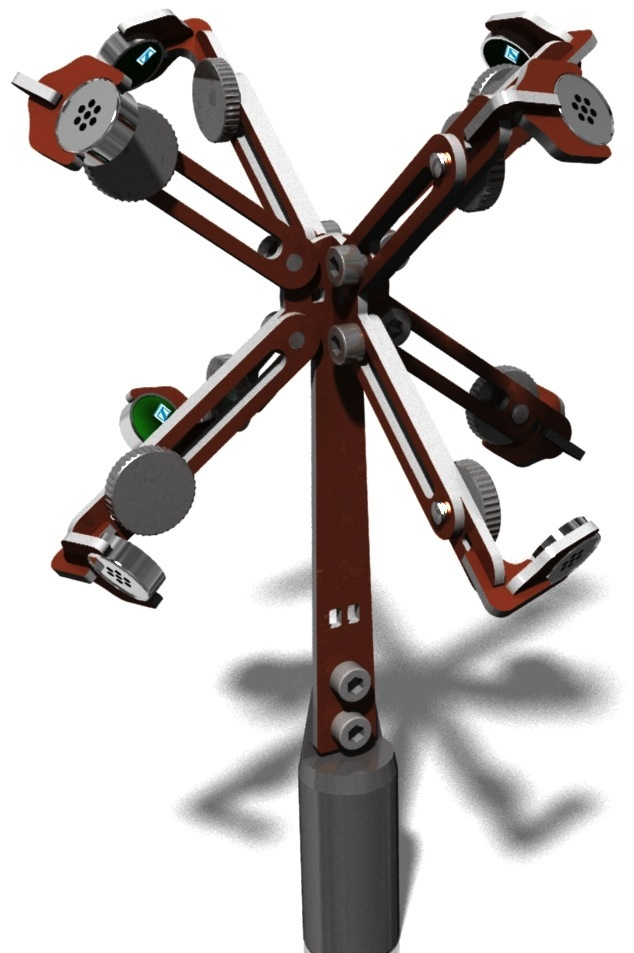
\includegraphics[width=\textwidth]{images/02_Konzeptionierung/3D_Konstruktion_Array_ohne_Kanten}
                \caption{3D Konstruktion}
                \label{fig:3D_Konstruktion_Array_ohne_Kanten}
        \end{subfigure}
        ~ %add desired spacing between images, e. g. ~, \quad, \qquad etc.
          %(or a blank line to force the subfigure onto a new line)
        \begin{subfigure}[b]{0.47\textwidth}
                \centering
                \includegraphics[width=\textwidth]{images/02_Konzeptionierung/Array_gefertigt}
                \caption{gefertigtes Array}
                \label{fig:Array_gefertigt}
        \end{subfigure}
        \caption{Vergleich zwischen 3D Konstruktion und Fertigungsergebnis}
        \label{fig:Vergleich_array_gefertigt}
\end{figure}
% ----------------------------------------- SUB-FIGURE ----------------------------------- 









% ****************************************************************************************
\section{Simulation}
\label{sec:Simulation}
% ****************************************************************************************
Zur Verifikation des in \Sec{sec:AnnahmenUndMatheZusammenhaenge} dargestellten mathematischen Modells wird eine umfangreiche Simulation in \matlab erstellt. Bezüglich der späteren Echtzeitimplementierung ist es notwendig, alle nötigen Programmfunktionen so zu erstellen, dass diese ebenfalls mit der zur Verfügung stehenden DSP- und C-Bibliothek umgesetzt werden können. Obwohl die Simulation nicht echtzeitkritisch ist, soll die Erfüllung des Echtzeitkriteriums bereits hier einen zentralen Punkt darstellen. Die Simulation beinhaltet folgende Komponenten:

\begin{enumerate}
    \item Ermittlung systembedingter Parameter %(wie \zB Winkelauflösung, Signalblocklänge, \dots)
    \item Erstellung synthetischer Signale
    \item Kreuzkorrelation unter Verwendung der FFT
    \item Algorithmus zur Berechnung des MCCC
    \item Optimierungsverfahren zur Ergebnis- und Geschwindigkeitsverbesserung
\end{enumerate}


% ***************************************************************************************
\subsection{Systemparameter}
\label{subsec:Systemparameter}
% ****************************************************************************************
Im Folgenden werden alle systembedingten Parameter ermittelt. Diese sind

\begin{itemize}
    \item Winkelauflösung inkl. Validierung des Winkelraums
    \item Anzahl abzusuchender Richtungen
    \item Signalblocklänge
    \item Anzahl der Kreuzkorrelationen
\end{itemize}





% ****************************************************************************************
\subsubsection{Winkelauflösung}
\label{subsubsec:Winkelaufloesung}
% ****************************************************************************************
Als grundsätzliche Anforderung an das System ist die mit der vorliegenden Hardware maximal zu erreichende Winkelauflösung abzubilden. Das heißt, je kleiner die Winkelauflösung (entspricht der Winkelschrittweite), desto größer ist die erreichbare Genauigkeit bei der Winkeldetektion. Da wie bereits erwähnt ein diskretes System realisiert wird, können nur Laufzeiten gemessen werden, die einem ganzzahligen Vielfachen der Abtastperiode $T_a$ entsprechen. Auf Grund dessen wird im Folgenden die Laufzeitdifferenz als SDOA\footnote{Sample Difference of Arrival} bezeichnet. Durch diese Zeitrasterung entsteht ebenfalls eine Winkelrasterung im Abstand der Winkelschrittweite, wodurch ein direkter Zusammenhang zwischen Winkelauflösung und verwendeter Systemabtastrate entsteht. Auf Grund der äquidistanten Anordnung benachbarter Sensoren ist die Winkelauflösung $\alpha_{\phi, \theta}$ für Azimuth- und Elevationswinkel identisch. $\alpha_{\phi, \theta}$ kann unter Verwendung von \Eq{ULA_1} und $d=d_{min}$ errechnet werden. $d_{min}$ beschreibt dabei die minimale Distanz zwischen zwei Mikrofonen. Durch Hinzufügen der Abtastperiode $T_a$ folgt $\alpha_{\phi, \theta}$ mit  


\begin{equation}
    \alpha_{\phi, \theta} = \frac{\pi}{2} - \arccos{\left( 1 \cdot T_a \cdot \frac{c}{d_{min}} \right)} 
\end{equation}

Der kleinste zu erreichende Winkelschritt hängt also direkt mit der kleinsten messbaren Laufzeitdifferenz von $1 \cdot T_a$ zusammen. \tab{Winkelaufloesung_Abtastfrequenz} zeigt mögliche Winkelauflösungen bei den im Audiobereich üblichen Abtastfrequenzen.



\begin{table}[h]
     \center
     \begin{tabular}{cc}
     \hline
          Abtastfrequenz [kHz] & Winkelauflösung [°] \\
           \hline \hline
          8                    & 47,9      \\
          16                   & 21,8      \\
          24                   & 14,3      \\
          48                   & 7,1       \\
          96                   & 3,5       \\
         \hline
     \end{tabular}
  \caption{Winkelauflösung bei unterschiedlichen Abtastfrequenzen}
 \label{tab:Winkelaufloesung_Abtastfrequenz}
 \end{table}



% ****************************************************************************************
\subsubsection{Validierung des Winkelraums} 
% ****************************************************************************************
Zur Validierung des abzubildenden Winkelraums ist es notwendig, jede mögliche Kombination aus Azimuth- und Elevationswinkel nachzumessen. Dazu wird ein Simulationsskript erstellt, das in Abhängigkeit vom eingestellten Winkelpaar den mittleren quadratischen Fehler $e_{rms}$ berechnet. Dieser ist geeignet, um die Abweichung eines Schätzers von dem zu schätzenden Wert zu ermitteln. Da die Schätzung jeder Richtung jeweils zwei Winkel liefert, werden die Fehler zunächst getrennt ermittelt. 

Der Fehler $e_{\phi | rms}$ für den Elevationswinkels $\phi$ ist gegeben durch


\begin{equation}\label{eq:rms_error_phi}
    e_{\phi | rms} = \sqrt{\frac{1}{M-1} \sum_{n=0}^{M-1} \vert \hat \phi_n - \phi \vert^2}.
\end{equation}


Für den Fehler $e_{\theta | rms}$ des Azimuthwinkel $\theta$ folgt so


\begin{equation}\label{eq:rms_error_theta}
    e_{\theta | rms} = \sqrt{\frac{1}{M-1} \sum_{n=0}^{M-1} \vert \hat \theta_n - \theta \vert^2}.
\end{equation}


Durch bilden des arithmetischen Mittelwerts resultiert der Gesamtfehler pro Richtung $\bar e_{\theta, \theta | rms}$ durch
\begin{equation}\label{eq:rms_error_phi_mid}
    \bar e_{\phi, \theta | rms} = \frac{e_{\phi | rms} + e_{\theta | rms}}{2}.
\end{equation}


\abb{algo_angle_error} zeigt das Flussdiagramm des Validierungsalgorithmus. Hier erfolgt die Wertvalidierung in einer dreifach geschachtelten Schleife. Für jedes Winkelpaar wird der gleiche Signalblock verwendet und in $M$ Unterblöcke geteilt. Diese werden alle entsprechend dem gewählten Winkelpaar synthetisch verzögert und nacheinander dem MCCC-Algorithmus zugeführt. Die Ergebnisse werden entsprechend den oben genannten Gleichungen verarbeitet und gespeichert. Der Algorithmus endet, wenn alle möglichen Winkelkombinationen durchlaufen wurden.


\myFigure{real}                  % Figure tag (missing, real)
         {veryVerySmall}                 % Size (small,medium,big)
         {h!}             % z.B. htbp
         {Algorithmus zur Validierung des abzubildenden Winkelraums}                % Figure title
         {algo_angle_error}                % Figure label 
         {02_Konzeptionierung/algo_angle_error}     % Path to real figure





\abb{angle_error} zeigt den Winkelfehler $e_{\phi | rms}$, $e_{\theta | rms}$ sowie $\bar e_{\theta, \theta | rms}$ in Abhängigkeit beider Raumwinkel. Als Quellensignal dient mittelwertfreies bandbegrenztes weißes Rauschen, mit einer Bandbreite von $B_{Noise} = 2700Hz$ im Bereich $300 Hz \leq f_{Noise} \leq 3000Hz$. Jeder Winkel wird mit einer Anzahl von $M=100$ Durchläufen simuliert. Die Auswertung der Fehlerkurven ergibt einen maximalen Fehler von:

\begin{equation*}
    \begin{array}{lll}
        e_{\phi | max} & = \displaystyle\max_{\phi,\theta}{ e_{\phi | rms}} & = 0,05° \\
        e_{\theta | max} & = \displaystyle\max_{\phi,\theta}{ e_{\theta | rms}} & = 0,4° \\
        \bar e_{\phi, \theta | max} & = \displaystyle\max_{\phi,\theta}{  \bar e_{\phi, \theta | rms}} & = 0,25°
    \end{array}
\end{equation*}

Auf Grund der sehr geringen Fehlerwerte kann davon ausgegangen werden, dass der Winkelraum innerhalb unter Berücksichtigung der Winkelschrittweite fehlerfrei abgebildet werden kann.


% OLD AND WRONG

%Zur Untersuchung des abzubildenden Winkelraums werden die Bereiche für den Elevationswinkel $\phi$ und den Azimuthwinkel $\theta$ getrennt betrachtet. \abb{AngleRes_Azimuth} zeigt die erreichbaren diskreten Laufzeitdifferenzen des Elevationswinkel über den gesamten Winkelraum. Betrachtet wurden hier die beiden untereinander liegenden Mikrofone $M_1$ und $M_5$ welche parallel zur Y-Achse positioniert sind. Analog zu \citet[S. 38]{Master_Array_Pikora} wirkt sich der Verlauf der Sinus-Funktion auf die zu erreichenden Winkel aus da die Steigung in Richtung $\frac{\pi}{2}$ \bzw $-\frac{\pi}{2}$ nicht-linear abnimmt. Bei den hier gegebenen Arrayabmaßen kann ein Winkelbereich von $-70° < \phi < 70°$ abgebildet werden. Da der Azimuthwinkel $\theta$ die Y-Achse rotiert bleibt er über den gesamten Bereich linear da sich bezüglich des betrachteten Mikrofonpaars keine Laufzeitdifferenz ergibt.

%\myFigure{real}                  % Figure tag (missing, real)
%         {medium}                 % Size (small,medium,big)
%         {position}             % z.B. htbp
%         {$K_{\phi}(\phi,\theta)$ zwischen Mikrofon $M_1$ und $M_5$ in Abhängigkeit von Azimuth- und Elevationswinkel bei einer Abtastfrequenz von $f_a = 48 kHz$}                % Figure title
%         {AngleRes_Azimuth}                % Figure label 
%         {02_Konzeptionierung/AngleRes_M1_M5}     % Path to real figure




 % ----------------------------------------- SUB-FIGURE -----------------------------------
\begin{figure}
        \centering
        \begin{subfigure}[b]{0.48\textwidth}
                \centering
                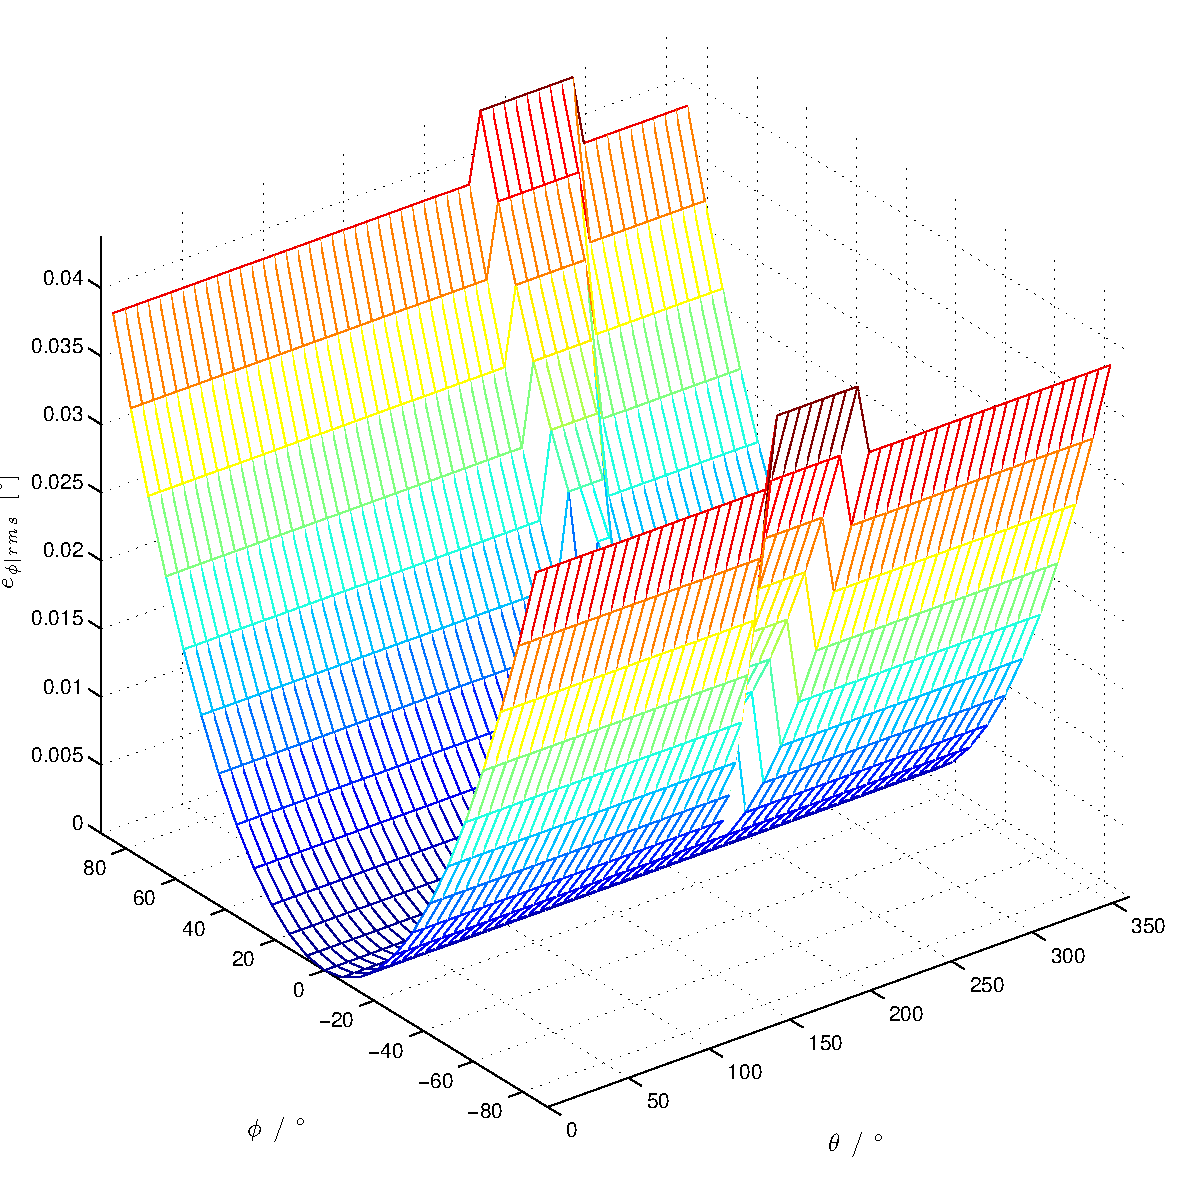
\includegraphics[width=\textwidth]{images/02_Konzeptionierung/angle_error_phi}
                \caption{$e_{\phi | rms}$}
                \label{fig:angle_error_phi}
        \end{subfigure}
        ~ %add desired spacing between images, e. g. ~, \quad, \qquad etc.
          %(or a blank line to force the subfigure onto a new line)
        \begin{subfigure}[b]{0.48\textwidth}
                \centering
                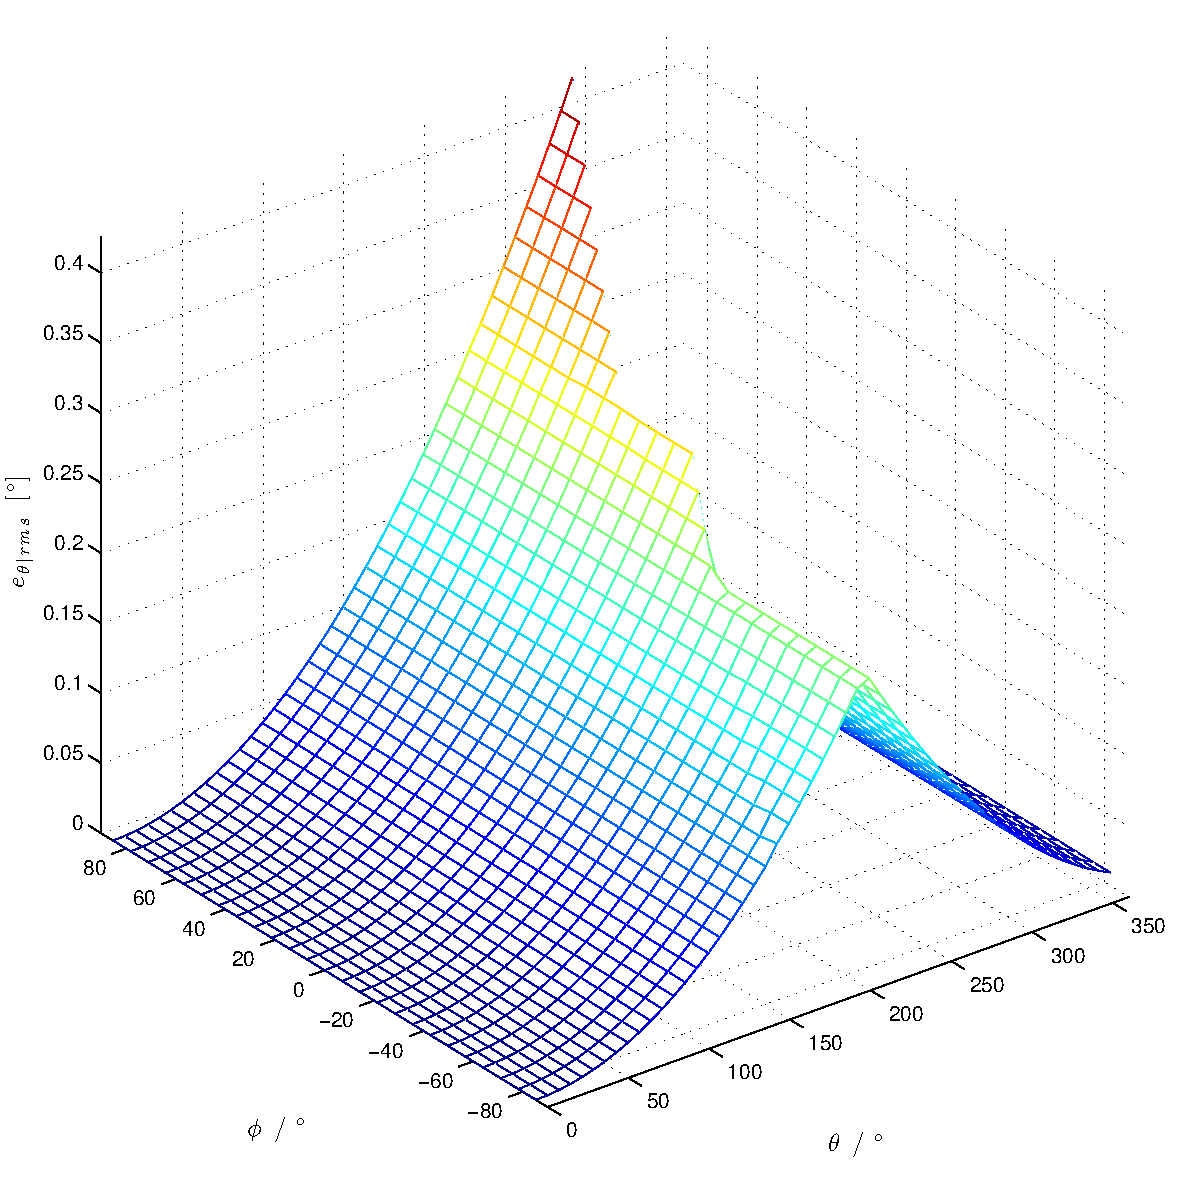
\includegraphics[width=\textwidth]{images/02_Konzeptionierung/angle_error_theta}
                \caption{$e_{\theta | rms}$}
                \label{fig:angle_error_theta}
        \end{subfigure}
        ~ %add desired spacing between images, e. g. ~, \quad, \qquad etc.
          %(or a blank line to force the subfigure onto a new line)
        \begin{subfigure}[b]{0.48\textwidth}
                \centering
                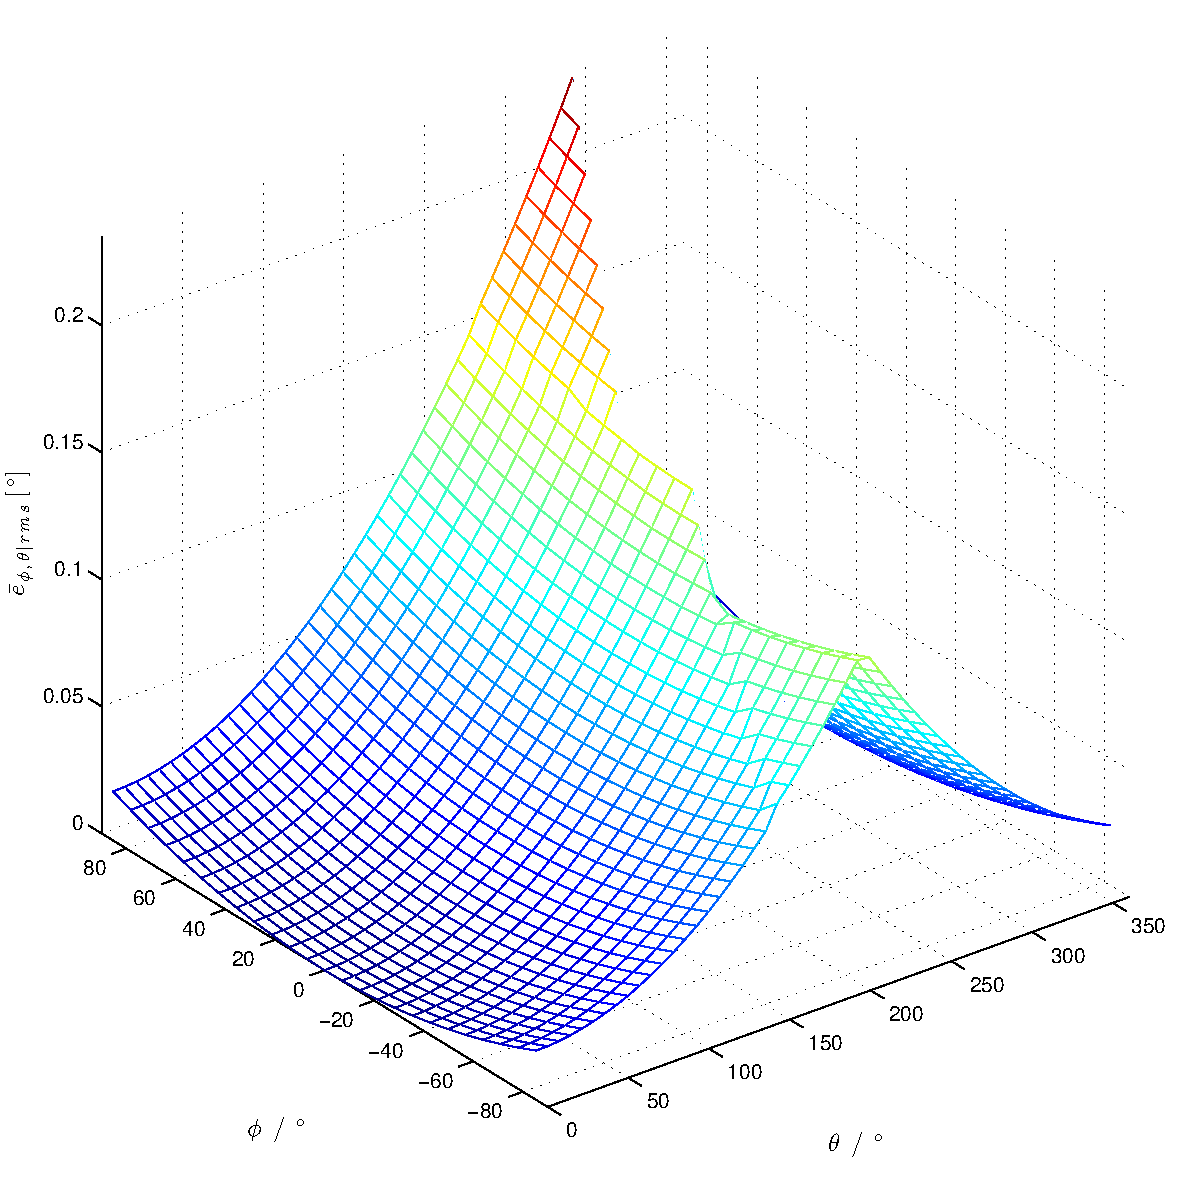
\includegraphics[width=\textwidth]{images/02_Konzeptionierung/angle_error_mid}
                \caption{$\bar e_{\phi, \theta | rms} = \frac{e_{\phi | rms} + e_{\theta | rms}}{2}$}
                \label{fig:angle_error_mid}
        \end{subfigure}
        \caption{Ergebnis der Winkelvalidierung für $e_{\phi | rms}$, $e_{theta | rms}$ und $\bar e_{\phi, \theta | rms}$ bei einer Abtastfrequenz von $f_a = 48 kHz$}
        \label{fig:angle_error}
\end{figure}
% ----------------------------------------- SUB-FIGURE ----------------------------------- 







%Zur Betrachtung des Azimuthbereiches werden die in der XY-Ebene liegenden Mikrofonpaare $M_1$ und $M_2$ (siehe \abb{AngleRes_Elevation_M12}) sowie $M_1$ und $M_4$ (siehe \abb{AngleRes_Elevation_M14}) untersucht. Die images zeigen erneut einen sinusförmigen Verlauf, nun allerdings in zwei Richtungen. Bei genauerer Betrachtung erkennt man jeweils in den Extremas der Funktion blinde Bereiche die erneut aus der abflachenden Steigung resultieren. Da die Mikrofonpaare jeweils parallel zu einer Achse der XY-Ebene verlaufen sind die Funktionen ebenfalls um $90°$ verschoben. %Da Verzögerungen zwischen diesen Mikrofonpaaren gleichzeitig gemessen und Verarbeitet werden können 

\subsubsection{Anzahl abzusuchender Richtungen}

Unter Verwendung der in \tab{Winkelaufloesung_Abtastfrequenz} angegebenen Winkelauflösungen sowie dem in \Sec{sec:Zielsetzung} genanten Winkelbereich für $\phi$ und $\theta$ ergeben sich die in \tab{Winkelanzahl_Abtastfrequenz} dargestellten Werte für die abzusuchenden Richtungen $S_{\phi,\theta}$. Der Suchaufwand wächst bei jeder Verdopplung der Abtastfrequenz überproportional an. Wie sich später zeigen wird, muss, um eine ausreichend hohe Winkelauflösung zu erreichen, ein optimiertes Suchverfahren entwickelt werden, wodurch das Echtzeitkriterium erfüllt wird. 



\begin{table}[h]
     \center
     \begin{tabular}{cccc }
     \hline
          Abtastfrequenz [kHz] & $N_{\phi}$ & $N_{\theta}$ & $S_{\phi,\theta} = N_{\phi} \cdot N_{\theta}$\\
           \hline \hline
          8                    & 4            & 8                & 32    \\
          16                   & 9            & 17               & 153    \\
          24                   & 13           & 26               & 338    \\
          48                   & 26           & 51               & 1326    \\
          96                   & 51           & 102              & 5202    \\
         \hline
     \end{tabular}
  \caption{Abzusuchende Richtungen $S_{\phi,\theta}$ bei unterschiedlichen Abtastfrequenzen}
 \label{tab:Winkelanzahl_Abtastfrequenz}
 \end{table}





%% ----------------------------------------- SUB-FIGURE -----------------------------------
%\begin{figure}
%        \centering
%        \begin{subfigure}[b]{0.48\textwidth}
%                \centering
%                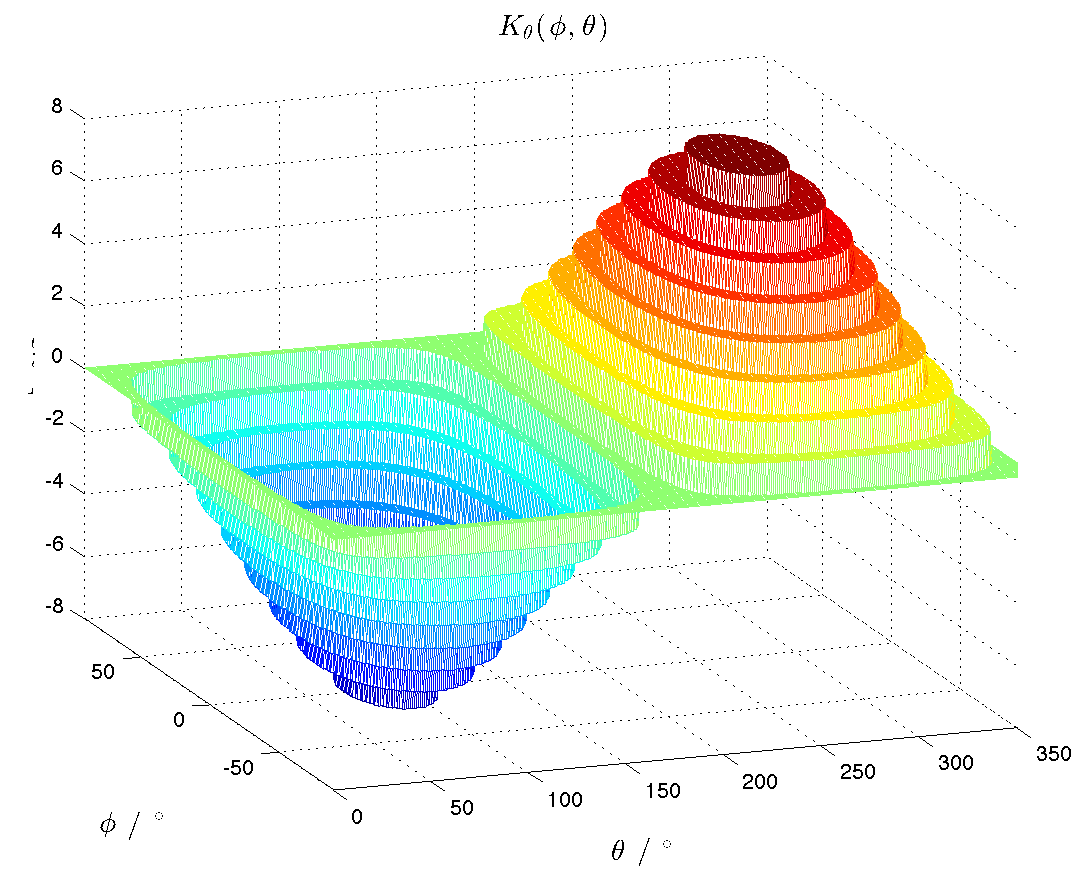
\includegraphics[width=\textwidth]{images/02_Konzeptionierung/AngleRes_M1_M2}
%                \caption{Mikrofon $M_1$ und $M_2$}
%                \label{fig:AngleRes_Elevation_M12}
%        \end{subfigure}
%        ~ %add desired spacing between images, e. g. ~, \quad, \qquad etc.
%          %(or a blank line to force the subfigure onto a new line)
%        \begin{subfigure}[b]{0.48\textwidth}
%                \centering
%                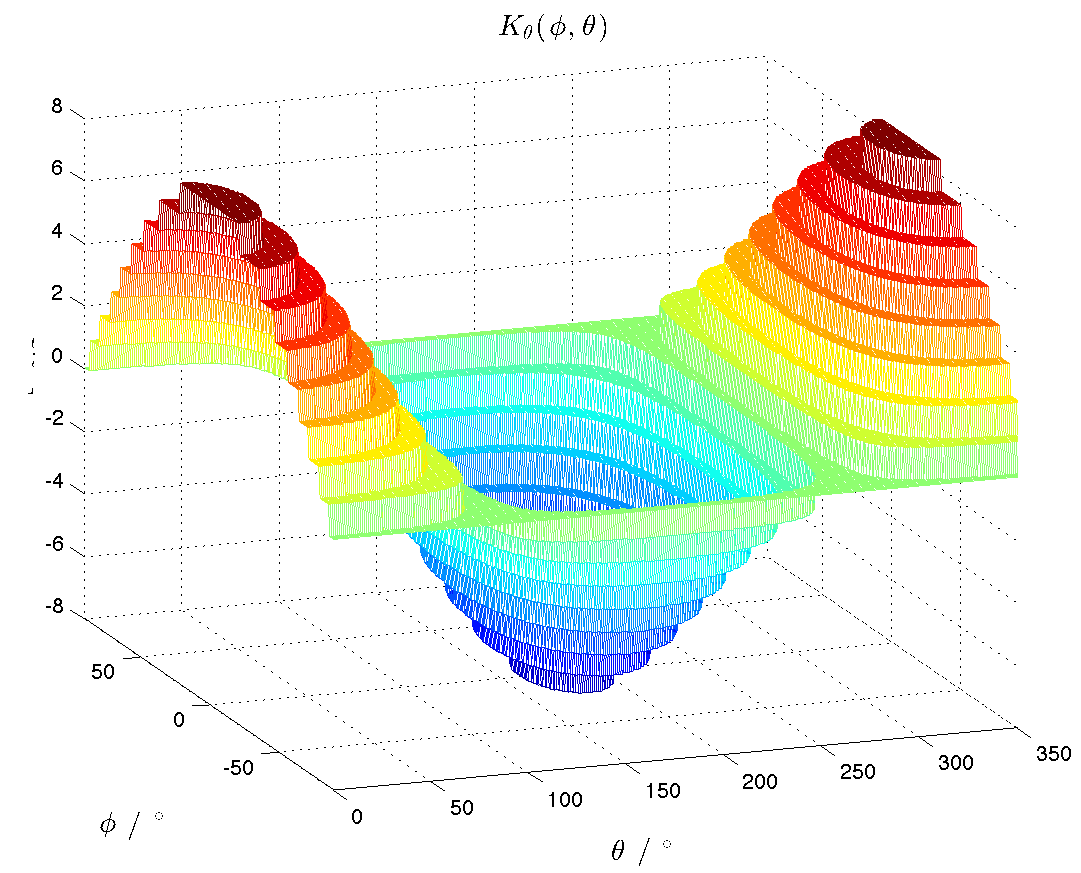
\includegraphics[width=\textwidth]{images/02_Konzeptionierung/AngleRes_M1_M4}
%                \caption{Mikrofon $M_1$ und $M_4$}
%                \label{fig:AngleRes_Elevation_M14}
%        \end{subfigure}
%        \stepcounter{missingFigureCount}
%        \caption{$K_{\theta}(\phi,\theta)$ in Abhängigkeit von Azimuth- und Elevationswinkel bei einer Abtastfrequenz von $f_a = 48 kHz$}
%        \label{fig:AngleRes_Elevation}
%\end{figure}
%% ----------------------------------------- SUB-FIGURE -----------------------------------

% ****************************************************************************************
\subsubsection{Signalblocklänge}
\label{subsubsec:Signalblocklaenge}
% ****************************************************************************************
Zum Festlegen der Signalblocklänge $L$ und somit auch der Fensterlänge $K$ der Kreuzkorrelation muss die maximale am Array messbare SDOA bestimmt werden. Diese entsteht an der hier verwendeten würfelförmigen Mikrofonanordnung genau dann, wenn der Elevationswinkel $\phi=\pm45°$ beträgt und der Azimuthwinkel $\theta$ sich im $45°$ Raster bewegt. In diesem Fall muss der Schall die Distanz $2 \cdot r$ zwischen zwei gegenüberliegenden Mikrofonen zurücklegen. Die maximale Verzögerung $K_{max}$ bezogen auf die Abtastfrequenz ergibt sich durch

\begin{equation}
    K_{max} = \frac{2r}{c} \cdot f_a
\end{equation}

\tab{Maximale_SDOA} zeigt die maximalen SDOA in Abhängigkeit verschiedener Abtastfrequenzen. 

\begin{table}[h]
     \center
     \begin{tabular}{cc}
     \hline
          Abtastfrequenz [kHz] & Maximale SDOA [Sample] \\
           \hline \hline
          8                    & $\pm$ 2      \\
          16                   & $\pm$ 5      \\
          24                   & $\pm$ 7      \\
          48                   & $\pm$ 14       \\
          96                   & $\pm$ 28       \\
         \hline
     \end{tabular}
  \caption{Maximale SDOA bei zwei gegenüberliegenden Mikrofonen}
 \label{tab:Maximale_SDOA}
 \end{table}




\myFigure{real}                  % Figure tag (missing, real)
         {medium}                 % Size (small,medium,big)
         {h!}             % z.B. htbp
         {Schalleinfallsrichtung mit der maximal messbaren Laufzeitdifferenz}                % Figure title
         {Maxinale_Laufzeit_Array}                % Figure label 
         {02_Konzeptionierung/Maximale_Laufzeit_Array}     % Path to real figure



Bei der Wahl der Signalblocklänge $L$ muss die maximale Verzögerung berücksichtigt werden. $L$ muss mindestens so groß gewählt werden, dass die maximal positive sowie maximal negative SDOA als Maximum im Korrelogramm sichtbar werden. Weiterhin sind die in \Sec{subsec:Kreuzkorrelation} genanten Kriterien im Bezug zur FFT einzuhalten. Die Signalblocklänge $L$ muss somit die halbe Länge der FFT-Länge $K$ besitzen. Weiterhin gilt für $K = 2^p$ und $p \in  \mathbb{N}^{+}$. Somit folgt für die Signalblocklänge $L = 2^{p-1}$.

% ****************************************************************************************
\subsubsection{Anzahl der Kreuzkorrelationen}
% ****************************************************************************************
Wie bereits in \Sec{subsec:MehrkanalKreuzkorrelationskoeffizient} erwähnt ist es notwendig, für die Ermittlung der Schalleinfallsrichtng die räumliche Korrelationsmatrix $\mathbf{R}_{\phi,\theta}$ zu erstellen. Dazu müssen zunächst alle nötigen Kreuzkorrelationsfunktionen berechnet werden. Anschließend werden diesen Funktionen Funktionswerte abhängig von den gewünschten Winkeln, entnommen um $\mathbf{R}_{\phi,\theta}$ zu erstellen. Da die Kreuzkorrelatinsfunktionen zwischen allen Mikrofonpaaren erstellt werden, ist deren Anzahl abhängig von der Mikrofonanzahl $N$. Auf Grund der Symmetrieeigenschaft von $\mathbf{R}_{\phi,\theta}$ müssen $\frac{N^2-N}{2}$  Kreuzkorrelationsfunktionen sowie $N$ Varianzen berechnet werden.



% ****************************************************************************************
\subsubsection{Wahl der Systemparameter}
\label{subsubsec:WahlSystemparateter}
% ****************************************************************************************
Nach der Untersuchung aller Systemparameter ist es nun notwendig, einen Satz von Parametern zu wählen, mit dem ein reales System auf einem DSP mit endlicher Rechenkapazität realisiert werden kann. Da auf Grund von Vorgaben die Anzahl der Mikrofone mit $N=8$ feststeht ergeben sich zur Berechnung $\frac{N^2-N}{2}$ = 28 Kreuzkorrelationen sowie 8 Varianzen. Ziel ist es, eine möglichst kleine Winkelauflösung zu erreichen. So wird die Abtastfrequenz des Systems mit $f_a=48kHz$ festgelegt, wodurch sich eine Winkelauflösung von $\alpha_{\phi, \theta}=7,1°$ ergibt. Nach \tab{Winkelanzahl_Abtastfrequenz} resultiert so eine Anzahl von $S_{\phi,\theta} = 1326$ abzusuchenden Richtungen, für jeweils die räumliche Korrelationsmatrix gebildet und dessen Determiante berechnet werden müssen. Auf Grund der Stationäritätseigenschaft von Sprachsignalen ist die Größe des Signalsblocks so klein wie möglich zu wählen. Gegenläufig dazu bewegt sich die benötigte Rechenzeit, welche den Wert 

\begin{equation}
    T_{calc_{max}} \leq \frac{L}{f_a} \leq L \cdot T_a
\end{equation}

nicht überschreiten darf. Die minimale Signalblocklänge beträgt bei dieser Abtastfrequenz $L=28$. In Bezug auf die DSP Implementierung wird der Signalblock auf eine Länge von $L=256$ gesetzt. Daraus ergibt sich ein Rechenfenster von $T_{calc_{max}} = 5,33ms$.



\begin{table}[h]
     \center
     \begin{tabular}{lcc}
     \hline
          Parameter & Variable & Wert \\
           \hline \hline
          Anzahl Mikrofone          & $N$                           & 8     \\
          Abtastfrequenz            & $f_a$                         & 48 kHz      \\
          Anzahl KKF                &  -                             & 28      \\
          Anzahl Varianz            &   -                            & 8       \\
          Winkelauflösung           & $\alpha_{\phi, \theta}$       & $7,1°$       \\
          Anzahl Suchrichtungen      & $S_{\phi,\theta}$             & $1326$        \\
          maximale Rechenzeit       & $T_{calc_{max}}$              & 5,33 ms         \\
         \hline
     \end{tabular}
  \caption{Gewählte Systemparameter im Überblick}
 \label{tab:Systemparameter}
 \end{table}




%\todo[inline]{Hier noch die entsprechende Abtastfrequenz wählen. Eingehen auf stationärität von Sprache (Signalblöcklänge), möglichst hohe Winkelauflösung, möglichst wenig abzusuchende Richtungen.}



% ****************************************************************************************
\subsection{Erstellung synthetischer Signale}
\label{subsec:ErstellungSynthetischerSignale}
% ****************************************************************************************
Zur Verifikation korrekter Algorithmusfunktionalität ist es notwendig, über Testsignale zu verfügen, bei denen genaue Kenntnis über die zu erwartenden Ergebnisse vorliegen. Am besten eignen sich dazu synthetisch erzeugte Signale. So lassen sich beliebige Testsignale für jede gewünschte Schalleinfallsrichtung für eine beliebige Anzahl von Mikrofonen erzeugen.

Wie in \Sec{subsec:Sensormodell} beschrieben, lassen sich zu jeder Schalleinfallsrichtung ($\phi, \theta$), bezogen auf das Referenzmikrofon, und jedem sich im Array befindenden Mikrofone jeweils eine Verzögerung zuordnen. Im Umkehrschluss kann so aus einem eindimesionalen Signalvektor ein $N+1$-Dimensionaler erzeugt werden in dem jedes der weiteren $N$ Mikrofone entsprechend einer gewünschten Schalleinfallsrichtung zeitlich verschoben wird. Diese Verschiebung kann mit dem Verschiebungssatz der Fourier-Transformation in \Eq{DFT_Verschiebung} erreicht werden, wobei der Parameter $N$ für die DFT-Länge steht \cite[S. 213]{Book_SigSys_Werner}.

\begin{equation}\label{eq:DFT_Verschiebung}
  x[n-m] \hspace{0.3cm} \overset{DFT}{\underset{N}{\longleftrightarrow}} \hspace{0.3cm} W^{mk}_N \cdot X[k]
\end{equation}

Zur Sicherstellung eines reelen Spektrums nach der Transformation kann die Symmetrieeigenschaft der Fourier-Transformation genutzt werden. Ist die Zeitfunktion gerade, d.h. $x[n] = x[-n]$, ergeben sich alle komplexen Anteile zu Null. Um dieses Verhalten auch bei ungeraden Funktionen zu erzwingen, wird die Folge an der Y-Achse gespiegelt. Nach der Multiplikation mit dem komplexen Verschiebungsterm und der Rücktransformation in den Zeitbereich können die gespiegelten Folgenelemente verworfen werden. \abb{Algo_Synthetisch_Zeitverschiebung} zeigt ein Flussdiagramm des implementierten Algorithmus. 




\myFigure{real}                  % Figure tag (missing, real)
         {small}                 % Size (small,medium,big)
         {h!}             % z.B. htbp
         {Algorithmus zur zeitlichen Verschiebung von N Signalen}                % Figure title
         {Algo_Synthetisch_Zeitverschiebung}                % Figure label 
         {02_Konzeptionierung/Algo_Synthetisch_Zeitverschiebung}     % Path to real figure




% ****************************************************************************************
\subsection{Kreuzkorrelation unter Verwendung der FFT}
\label{subsec:KreuzkorrelationVerwendungFFT}
% ****************************************************************************************
Der Ablauf zur Berechnung der $\frac{N^2-N}{2}$ Kreuzkorrelationsfunktionen sowie der $N$ Varianzen ist in \abb{Algo_CC_Var} dargestellt. Im Vergleich zur beschriebenen Mathematik in \Sec{subsec:MehrkanalKreuzkorrelationskoeffizient} werden die Sensorsignale vor der Korrelation nicht entsprechend einer Schalleinfallsrichtung zeitlich zueinander ausgerichtet. Grund hierfür ist der enorme Rechenaufwand der dadurch entstehen würde. Der Berechnungsvorgang der Kreuzkorrelation müsste in diesem Fall entsprechend der angegebenen Anzahl von Richtungen $S_{\phi,\theta}$ in \tab{Winkelanzahl_Abtastfrequenz} wiederholt werden, wodurch sich eine Echtzeitimplementierung als schwierig erweist. Da sich die Zeitverzögerung zwischen einem Signal und dessen verschobener Kopie in der Position der Kreuzkorrelationsfunktionen auf dessen Zeitachse widerspiegelt, kann die Verschiebung der Zeitsignale vor der Korrelation oder die Verschiebung des Korrelogramms nach der Korrelation um jeweils die selbe Zeit als äquivalent betrachtet werden. Unter Anwendung der Korrelogrammverschiebung kann Rechenzeit eingespart werden, da die oben angegebene Anzahl von Korrelationsoperationen nur einmal pro Signalblock berechnet werden muss.

 


%Die Berechnung der Varianzen läuft in einer einfach geschachtelten schleife ab wobei zur Ermittlung der Korrelationsfunktionen zwischen jedem Sensorpaar eine doppelt geschachtelte schleife nötig ist.




\myFigure{real}                                                   % Figure tag (missing, real)
         {veryVerySmall}                                                       % Size (small,medium,big)
         {h!}                                                  % z.B. htbp
         {Algorithmus zur Berechnung der nötigen Kreuzkorrelationsfunktionen $r_{y_i, y_j}$ sowie Varianzen $\sigma^2_{y_n}$}    % Figure title
         {Algo_CC_Var}                                               % Figure label 
         {02_Konzeptionierung/Algo_CC_Var}                           % Path to real figure

% ****************************************************************************************
\subsection{Algorithmus zur Berechnung des MCCC}
% ****************************************************************************************
\abb{Algo_MCCC} zeigt den Ablauf zur Berechnung des Mehrkanal-Kreuzkorrelationskoeffizienten. Zu Beginn wird abhängig vom Azimuth- und Elevationswinkel die räumliche Korrelationsmatrix  $\mathbf{R}_{\phi,\theta}$ gebildet. Wie bereits in \Sec{subsec:KreuzkorrelationVerwendungFFT} erwähnt, erfolgt dies durch Korrelogrammverschiebung unter Verwendung von $f_n(\phi, \theta)$ mit $\mathbf{R}_{\phi,\theta}=$

\begin{equation}
    \begin{bmatrix}
    \sigma_{y_0}^2	     & r_{y_0 y_1}(k + f_1(\phi,\theta))     & \dots & r_{y_0 y_N}(k + f_N(\phi,\theta))       \\
    r_{y_0 y_1}(k + f_1(\phi,\theta))	  & \sigma_{y_1}^2      & \dots & r_{y_1 y_N}(k + f_N(\phi,\theta) - f_1(\phi,\theta))        \\
    \vdots	            & \vdots 	           & \ddots & \vdots                \\
    r_{y_0 y_N}(k + f_N(\phi,\theta))	  & r_{y_1 y_N}(k + f_N(\phi,\theta) - f_1(\phi,\theta))     & \dots	 & \sigma_{y_N}^2
    \end{bmatrix}
\end{equation}



Anschließend erfolgt die Berechnung der Determinante, wobei dessen Wert in einem separaten zweidimensionalen Feld $det_{\phi, \theta}$ abgelegt wird. Dieser Vorgang wird entsprechend den Angaben in \tab{Winkelanzahl_Abtastfrequenz} für jede messbare Richtung wiederholt. Abschließend wird das Minimum von $det_{\phi, \theta}$ ermittelt und der entsprechenden Richtung zugeordnet.

\abb{Sim_Synthetic_dB} zeigt das Ergebnis der MCCC-Simulation mit Verwendung eines synthetisch verzögerten Sprachsignals bei zwei unterschiedlichen Schalleinfallsrichtungen sowie SNR\footnote{Signal-Rausch-Verhältnis}. Das Sprachsignal wurde dabei mit unkorreliertem weißen Rauschen entsprechend angegebenem SNR überlagert. Zu erkennen ist, dass die Richtung auch bei geringem SNR gut detektiert werden kann.



%Zu beachten ist, dass die Anzahl der Determinantenberechnung mit wachsender Winkelauflösung stark ansteigt. 

\myFigure{real}                                                   % Figure tag (missing, real)
         {veryVerySmall}                                                       % Size (small,medium,big)
         {h!}                                                  % z.B. htbp
         {Algorithmus zur Berechnung des Mehrkanal-Kreuzkorrelations-koeffizienten}    % Figure title
         {Algo_MCCC}                                               % Figure label 
         {02_Konzeptionierung/Algo_MCCC}                           % Path to real figure

       
 % ----------------------------------------- SUB-FIGURE -----------------------------------
\begin{figure}
        \centering
        \begin{subfigure}[b]{0.48\textwidth}
                \centering
                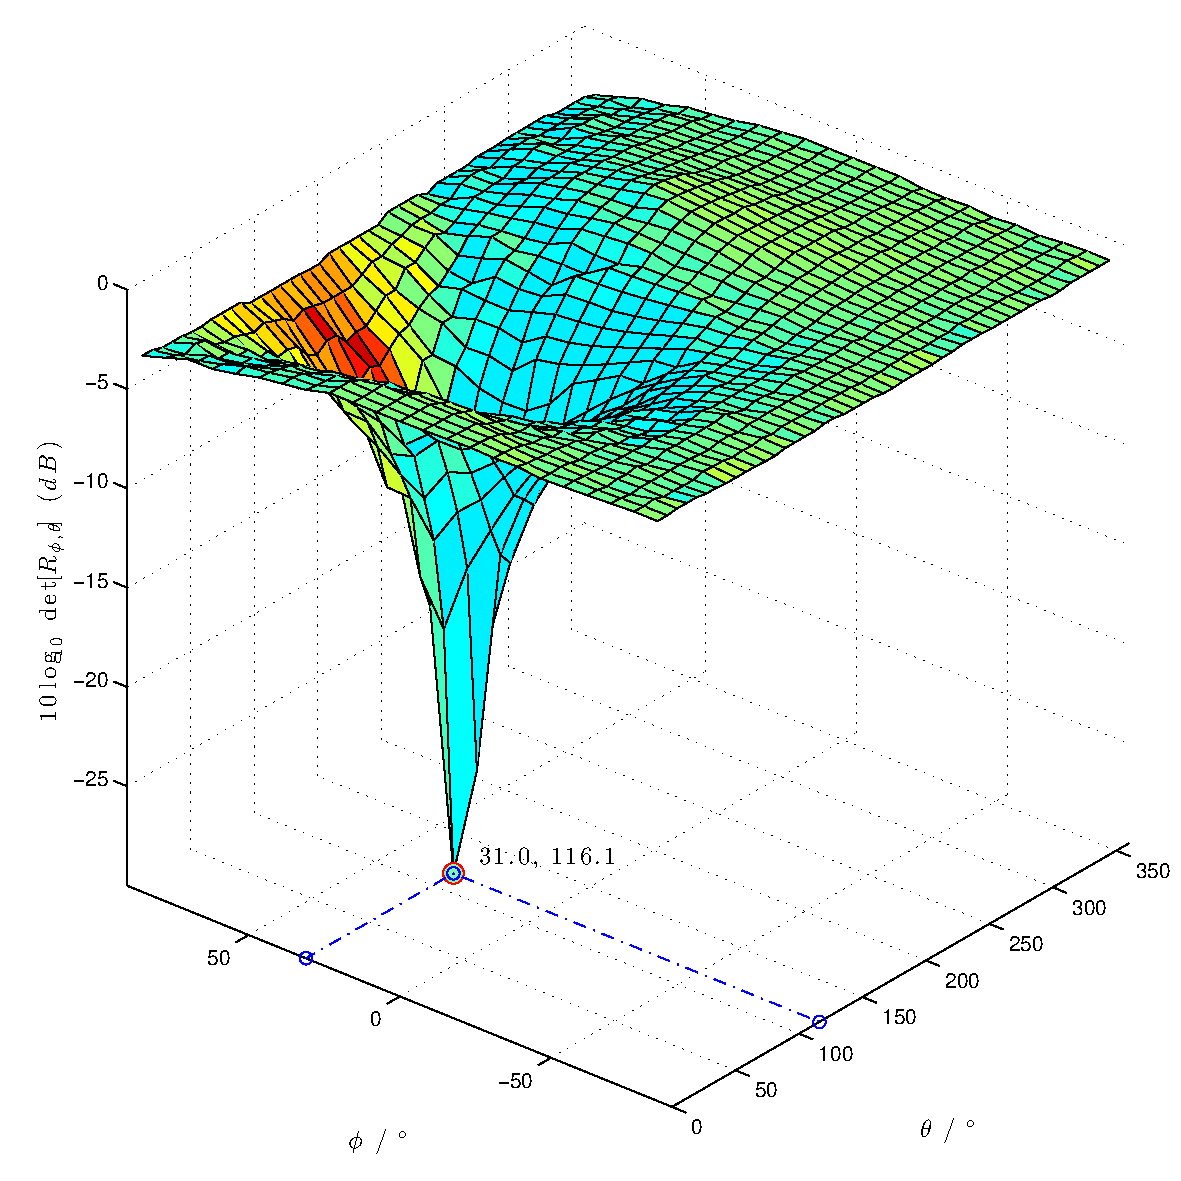
\includegraphics[width=\textwidth]{images/02_Konzeptionierung/Sim_voice_Phi_30_Theta_120_SNR_100dB_log}
                \caption{$\phi=30°,\theta=120°, \mathrm{SNR}=100dB$}
                \label{fig:Sim_Phi_30_Theta_120_dB}
        \end{subfigure}
        ~ %add desired spacing between images, e. g. ~, \quad, \qquad etc.
          %(or a blank line to force the subfigure onto a new line)
        \begin{subfigure}[b]{0.48\textwidth}
                \centering
                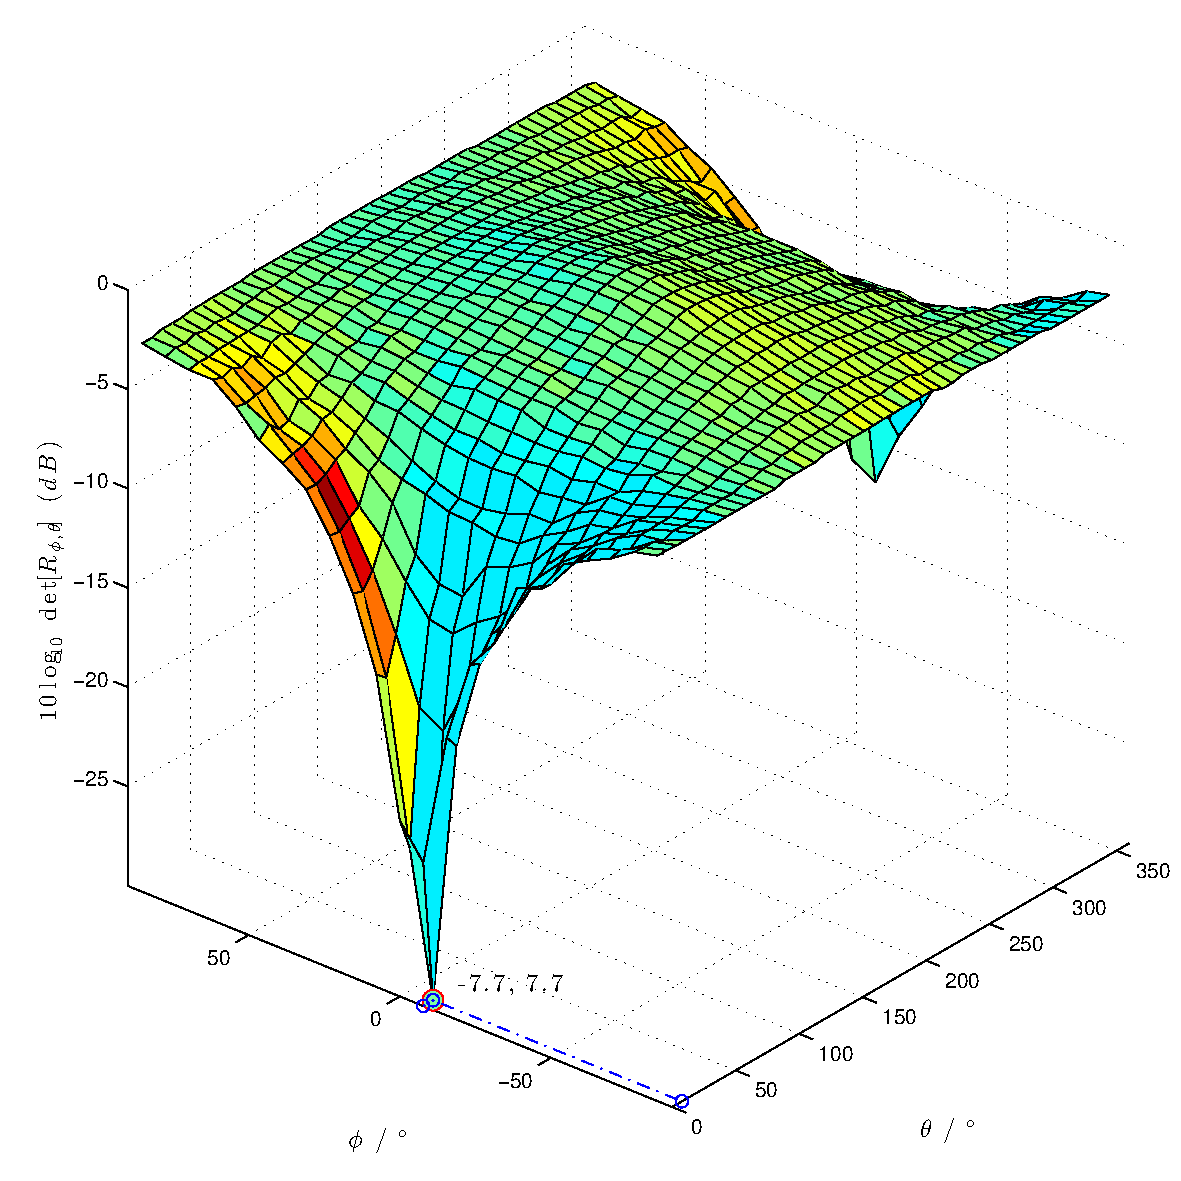
\includegraphics[width=\textwidth]{images/02_Konzeptionierung/Sim_voice_Phi_-7_Theta_7_SNR_100dB_log}
                \caption{$\phi=-7°,\theta=7°, \mathrm{SNR}=100dB$}
                \label{fig:Sim_Phi_-7_Theta_7_dB}
        \end{subfigure}
        ~ %add desired spacing between images, e. g. ~, \quad, \qquad etc.
          %(or a blank line to force the subfigure onto a new line)
        \begin{subfigure}[b]{0.48\textwidth}
                \centering
                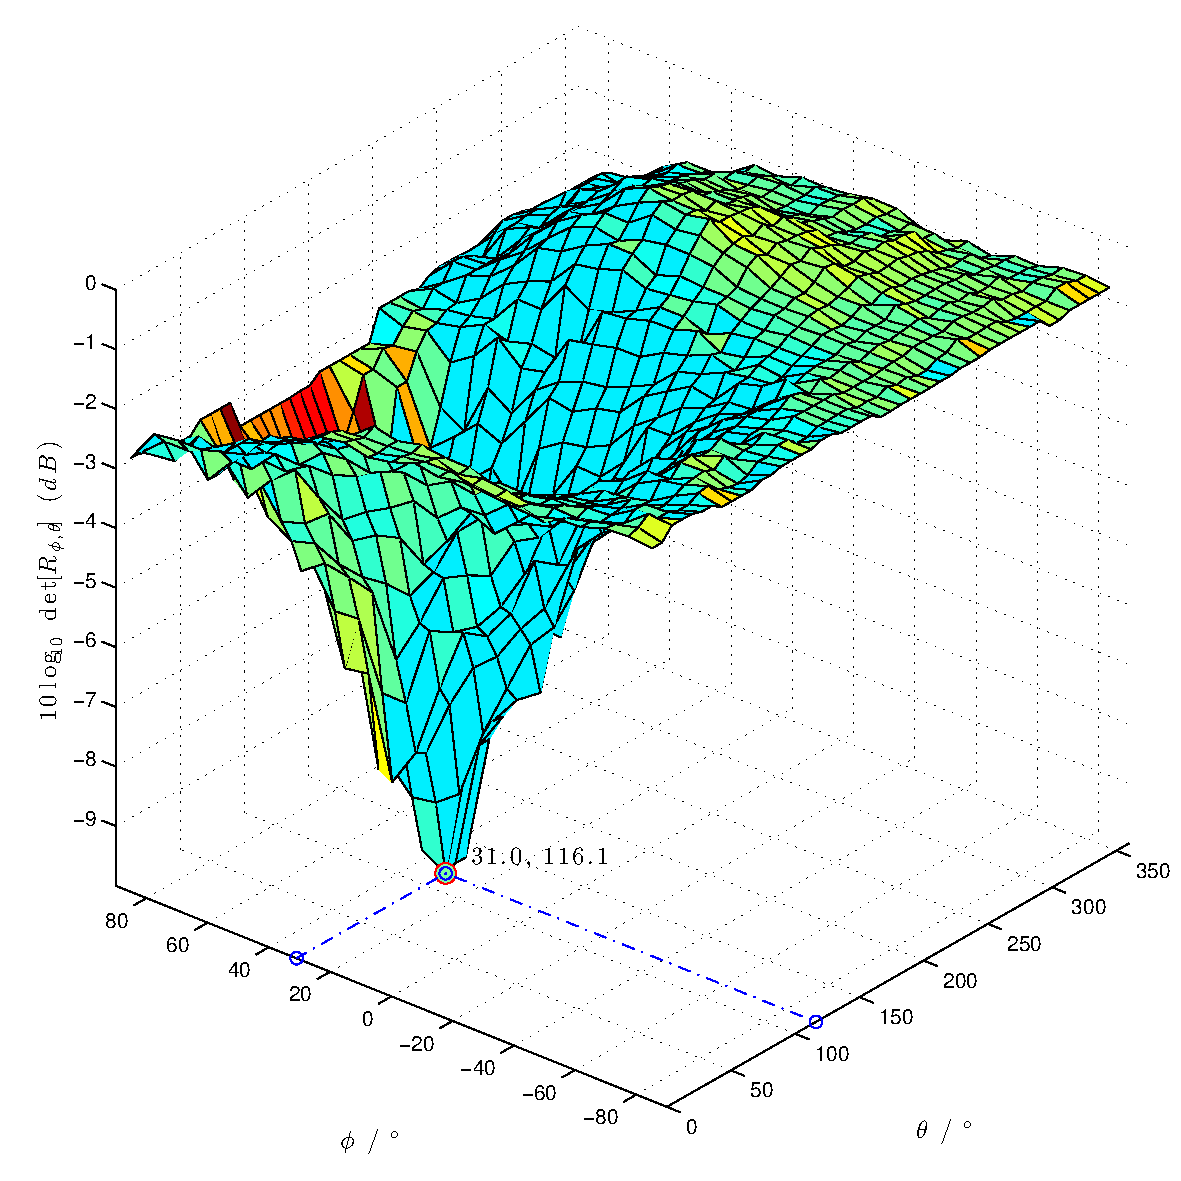
\includegraphics[width=\textwidth]{images/02_Konzeptionierung/Sim_voice_Phi_30_Theta_120_SNR_5dB_log}
                \caption{$\phi=30°,\theta=120°, \mathrm{SNR}=5dB$}
                \label{fig:Sim_Phi_30_Theta_120_dB_SNR_5dB}
        \end{subfigure}
        ~ %add desired spacing between images, e. g. ~, \quad, \qquad etc.
          %(or a blank line to force the subfigure onto a new line)
        \begin{subfigure}[b]{0.48\textwidth}
                \centering
                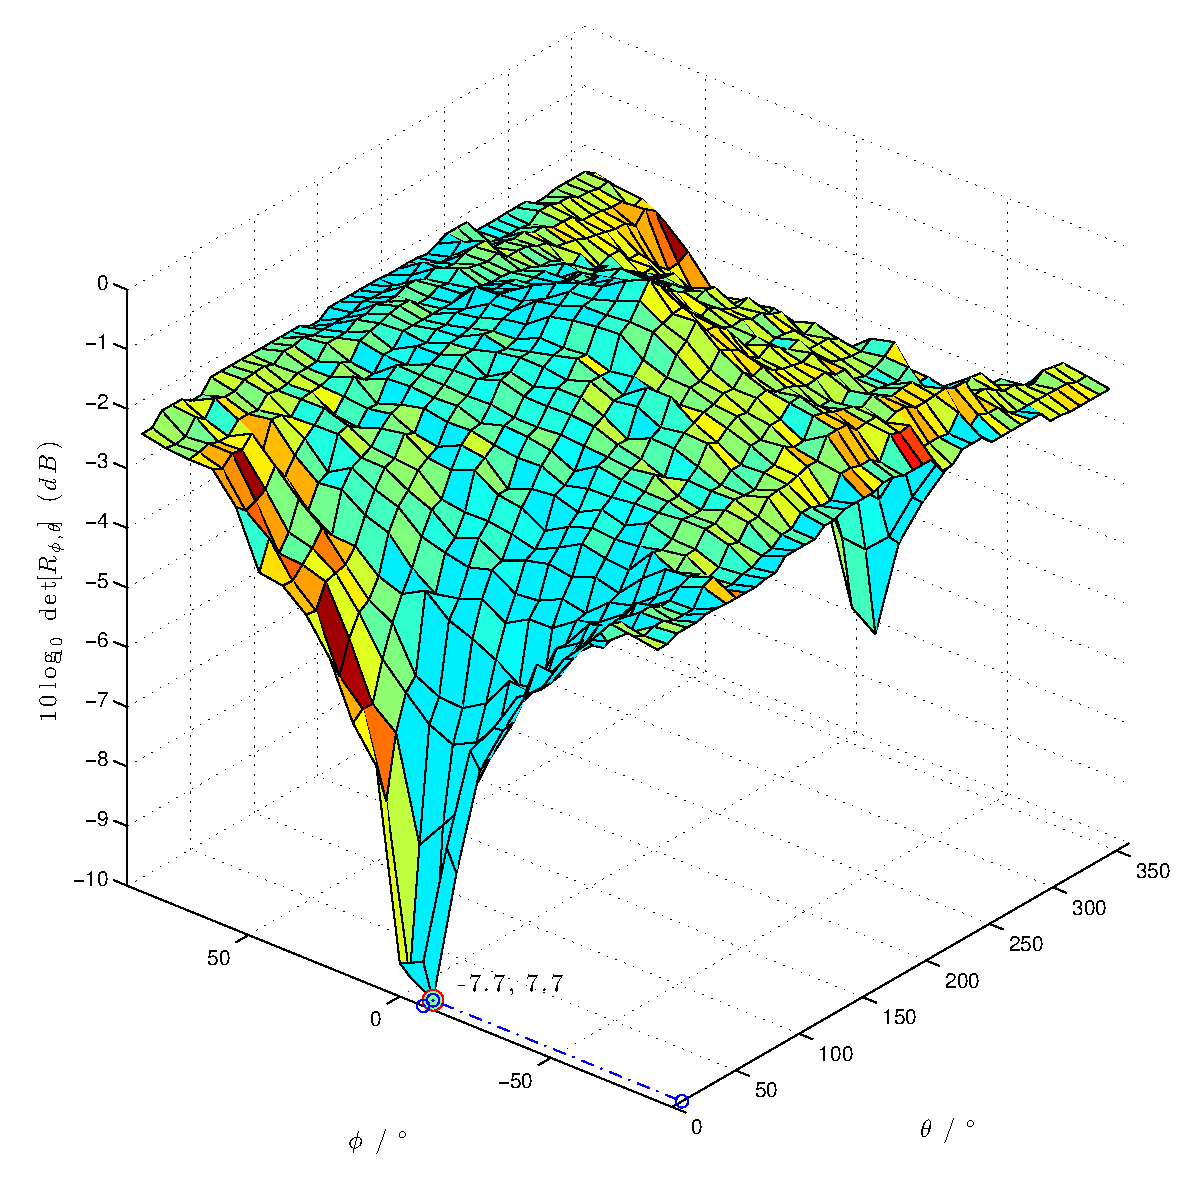
\includegraphics[width=\textwidth]{images/02_Konzeptionierung/Sim_voice_Phi_-7_Theta_7_SNR_5dB_log}
                \caption{$\phi=-7°,\theta=7°, \mathrm{SNR}=5dB$}
                \label{fig:Sim_Phi_-7_Theta_7_dB_SNR_5dB}
        \end{subfigure}
        \caption{Ergebnis des MCCC unter Verwendung eines synthetisch verzögerten Sprachsignals bei zwei unterschiedlichen Schalleinfallsrichtungen sowie SNR und einer Abtastfrequenz von $f_a=44,1kHz$.}
        \label{fig:Sim_Synthetic_dB}
\end{figure}
% ----------------------------------------- SUB-FIGURE -----------------------------------        
         
Zur Untersuchung des Korrelationsverfahrens auf die Entstehung des räumlichen Aliasing-Effekts wird die Reaktion des Systems auf ein rein periodisches Signal der Form $y[n] = \sin{\left( 2 \pi \frac{f}{f_a} n \right)}$ bei unterschiedlichen Frequenzen beobachtet. \abb{Sim_sine_spartial_aliasing} illustriert sechs Ergebnisse der MCCC im Frequenzintervall $100 Hz \leq f \leq 3kHz$. Zu sehen ist, dass sich die Ausprägung des Minimums bei steigender Frequenz deutlich verbessert. Grund hierfür ist die immer schmaler werdende Hauptkeule der Kreuzkorrelationsfunktion wie in \abb{Sim_sine_r_xy} dargestellt. Weiterhin treten in \abb{Sim_sine_spartial_aliasing} zusätzliche lokale Minima auf, deren Anzahl und Abstand von der Menge sowie Höhe der Nebenkeulen im Suchbereich (zwischen den grünen Linien in \abb{Sim_sine_r_xy}) abhängt. Bei Verletzten des Kriteriums in \Eq{raemlichesAliasing} befinden sich mehrere Spitzen innerhalb des Suchbereichs der KKF, was die Lokalisierung des korrekten Maximums erschwert. Auf Grund der hier verwendeten nicht erswartungstreuen Schätzung (siehe \Sec{subsubsec:ErwartungstreueSchaetzung}) erfährt die Kreuzkorrelation eine Gewichtung durch das Dreieckfenster, so dass die Nebenmaxima gedämpft werden und die Wahrscheinlichkeit der Entstehung von räumlichem Aliasing deutlich verringert wird.



% ----------------------------------------- SUB-FIGURE -----------------------------------
\begin{figure}
        \centering
        \begin{subfigure}[b]{0.48\textwidth}
                \centering
                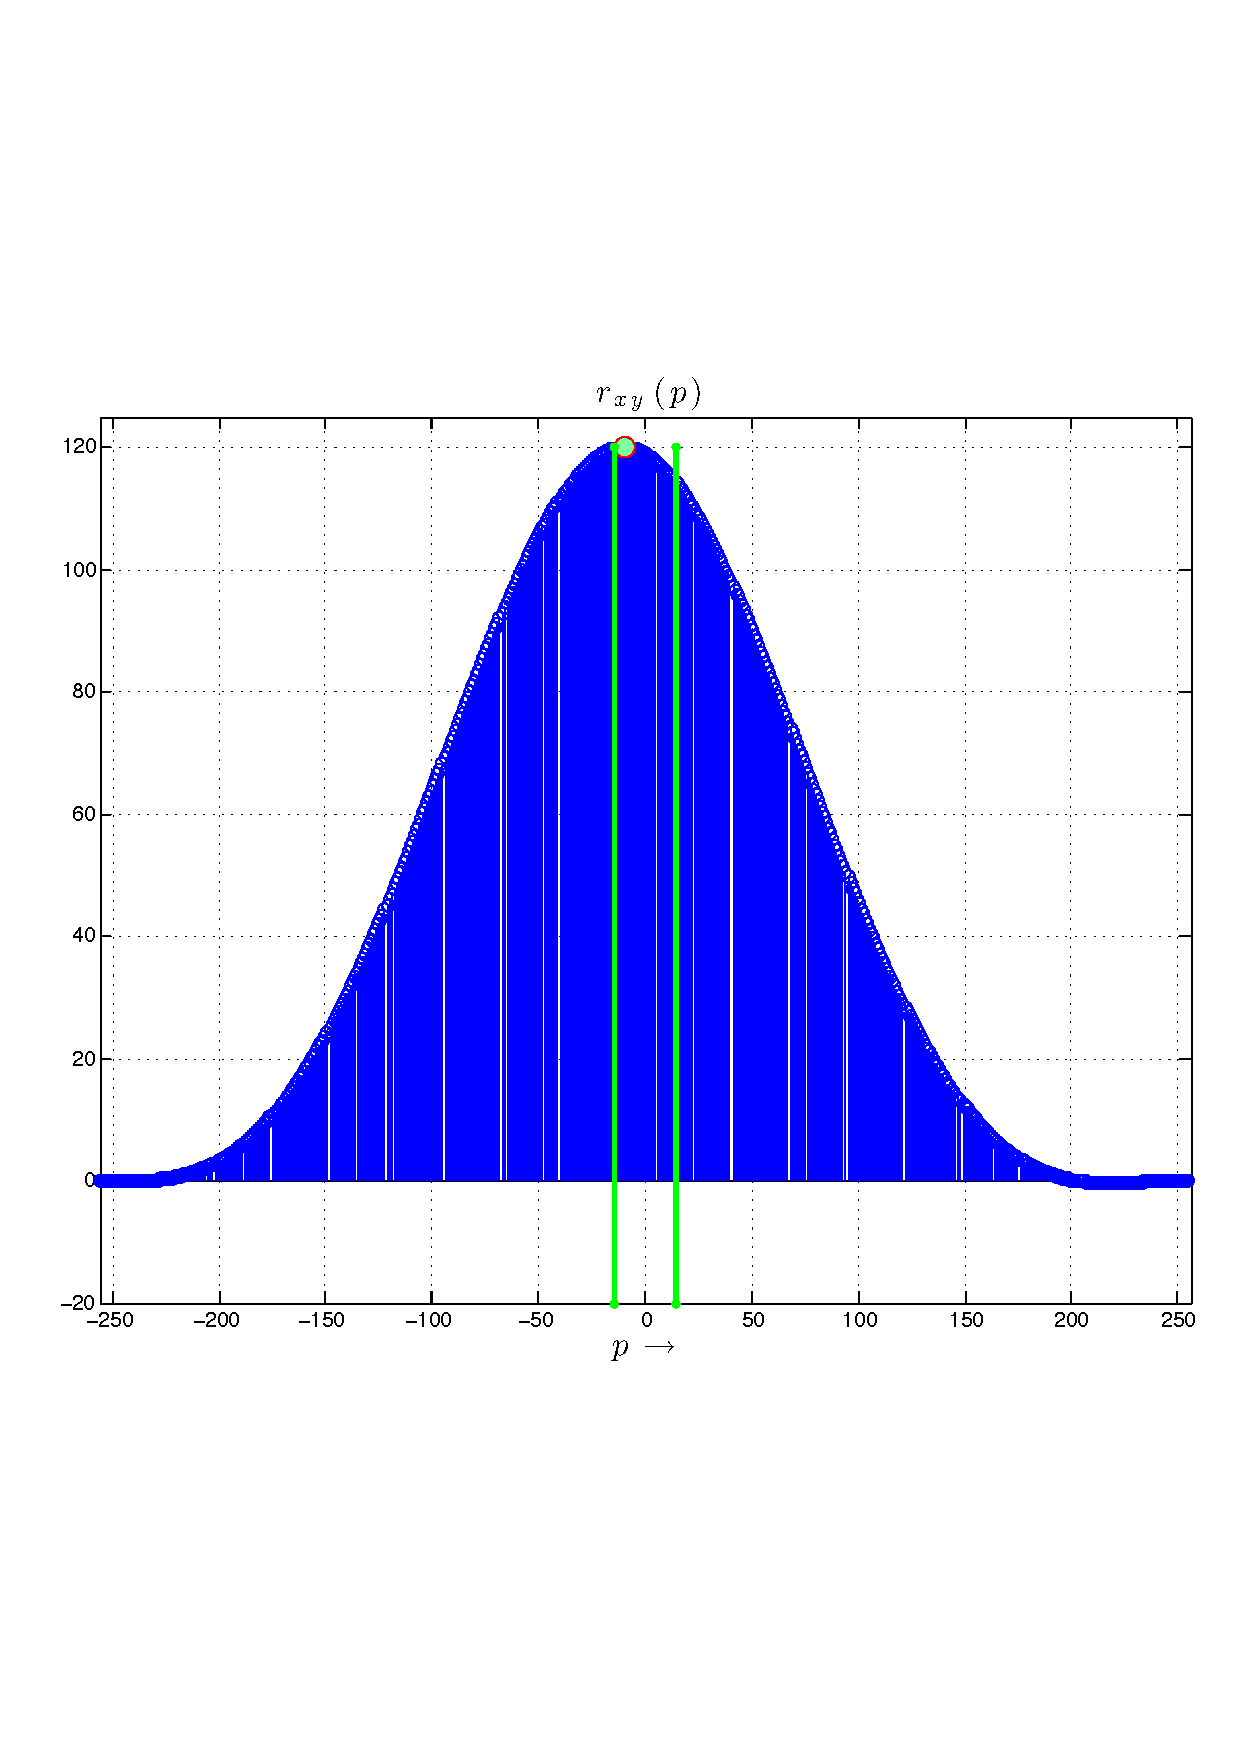
\includegraphics[width=\textwidth]{images/02_Konzeptionierung/sine_rxy_f_100}
                \caption{$f=100Hz$}
                \label{fig:sine_rxy_f_100}
        \end{subfigure}
        ~ %add desired spacing between images, e. g. ~, \quad, \qquad etc.
          %(or a blank line to force the subfigure onto a new line)
        \begin{subfigure}[b]{0.48\textwidth}
                \centering
                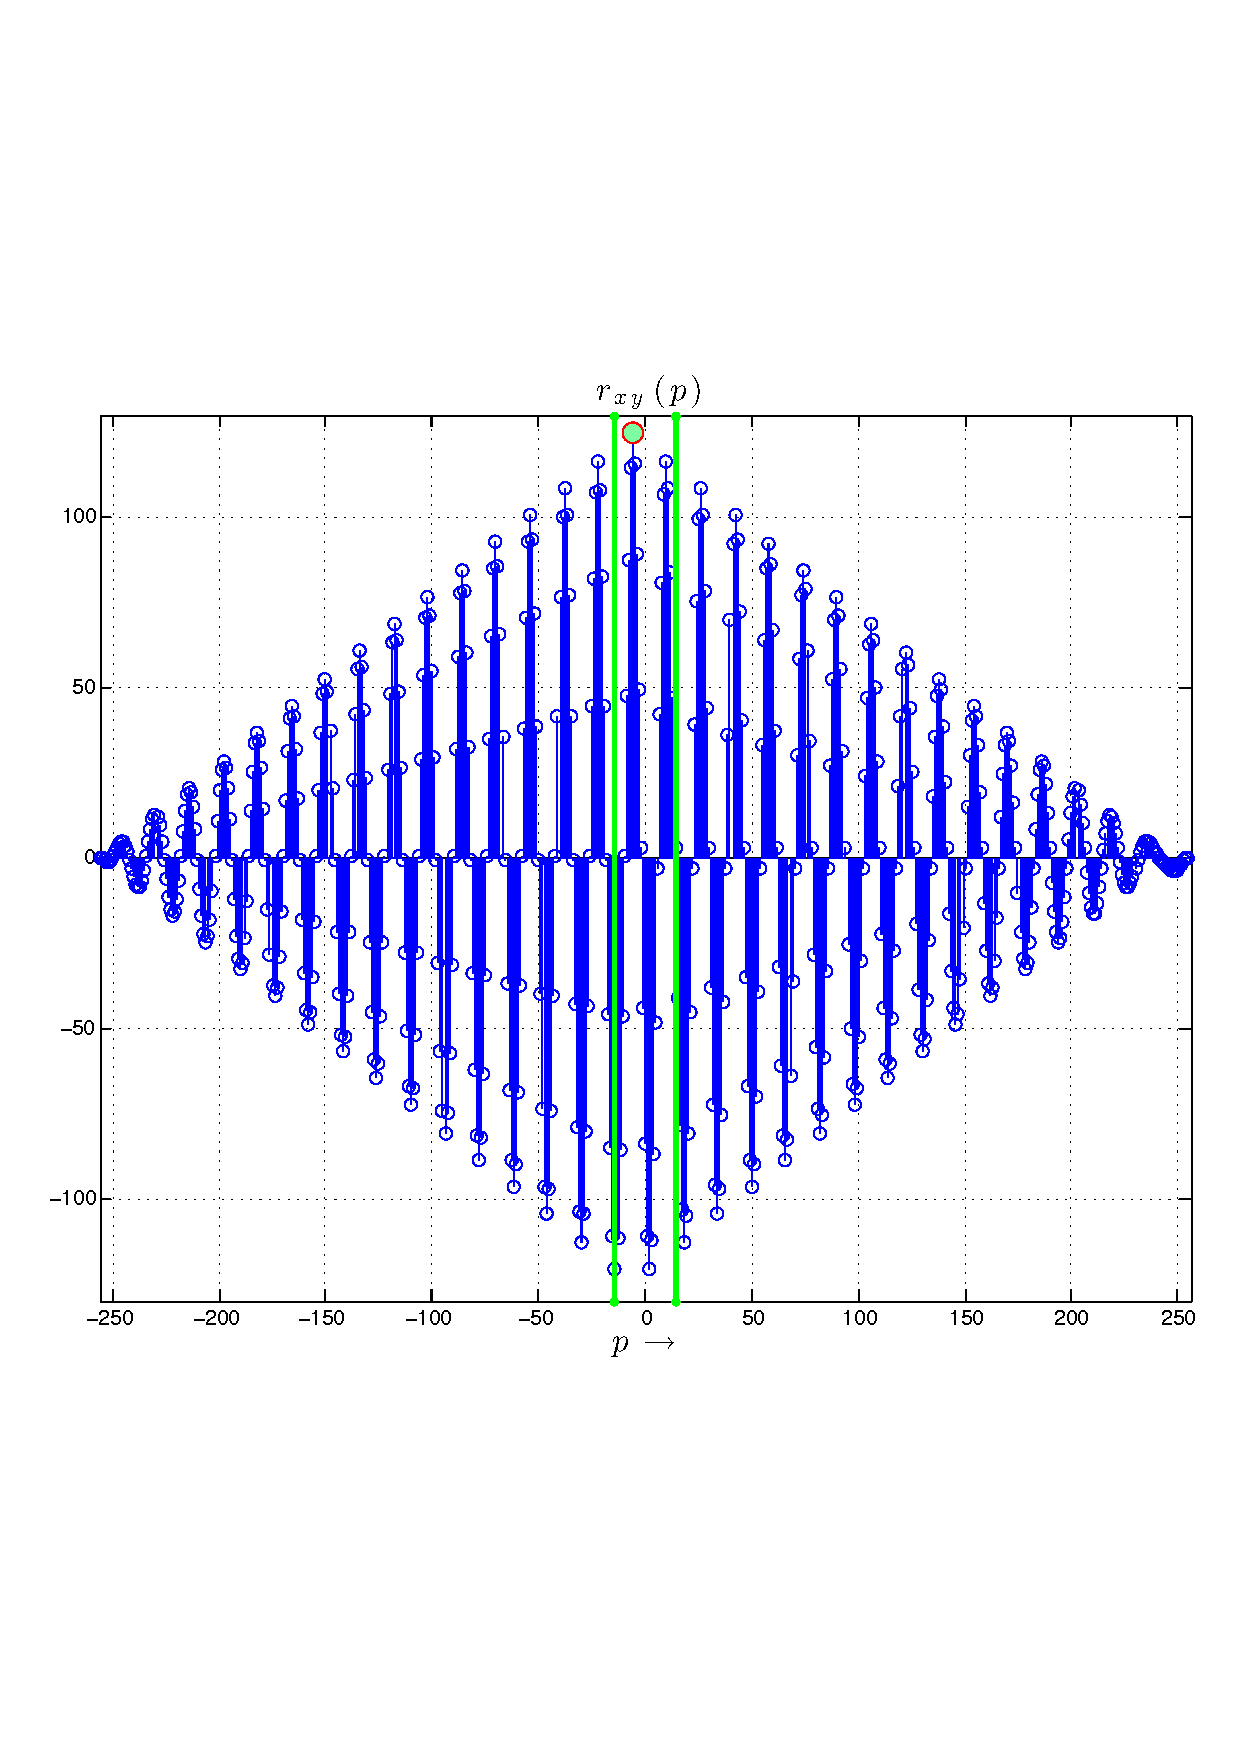
\includegraphics[width=\textwidth]{images/02_Konzeptionierung/sine_rxy_f_3000}
                \caption{$f=3000Hz$}
                \label{fig:sine_rxy_f_3000}
        \end{subfigure}
        \caption{Ergebnis der Kreuzkorrelations unter Verwendung eines synthetisch verzögerten Sinussignals bei einer Abtastfrequenz von $f_a=48kHz$.}
        \label{fig:Sim_sine_r_xy}
\end{figure}
% ----------------------------------------- SUB-FIGURE -----------------------------------

  
 % ----------------------------------------- SUB-FIGURE -----------------------------------
\begin{figure}
        \centering
        \begin{subfigure}[b]{0.48\textwidth}
                \centering
                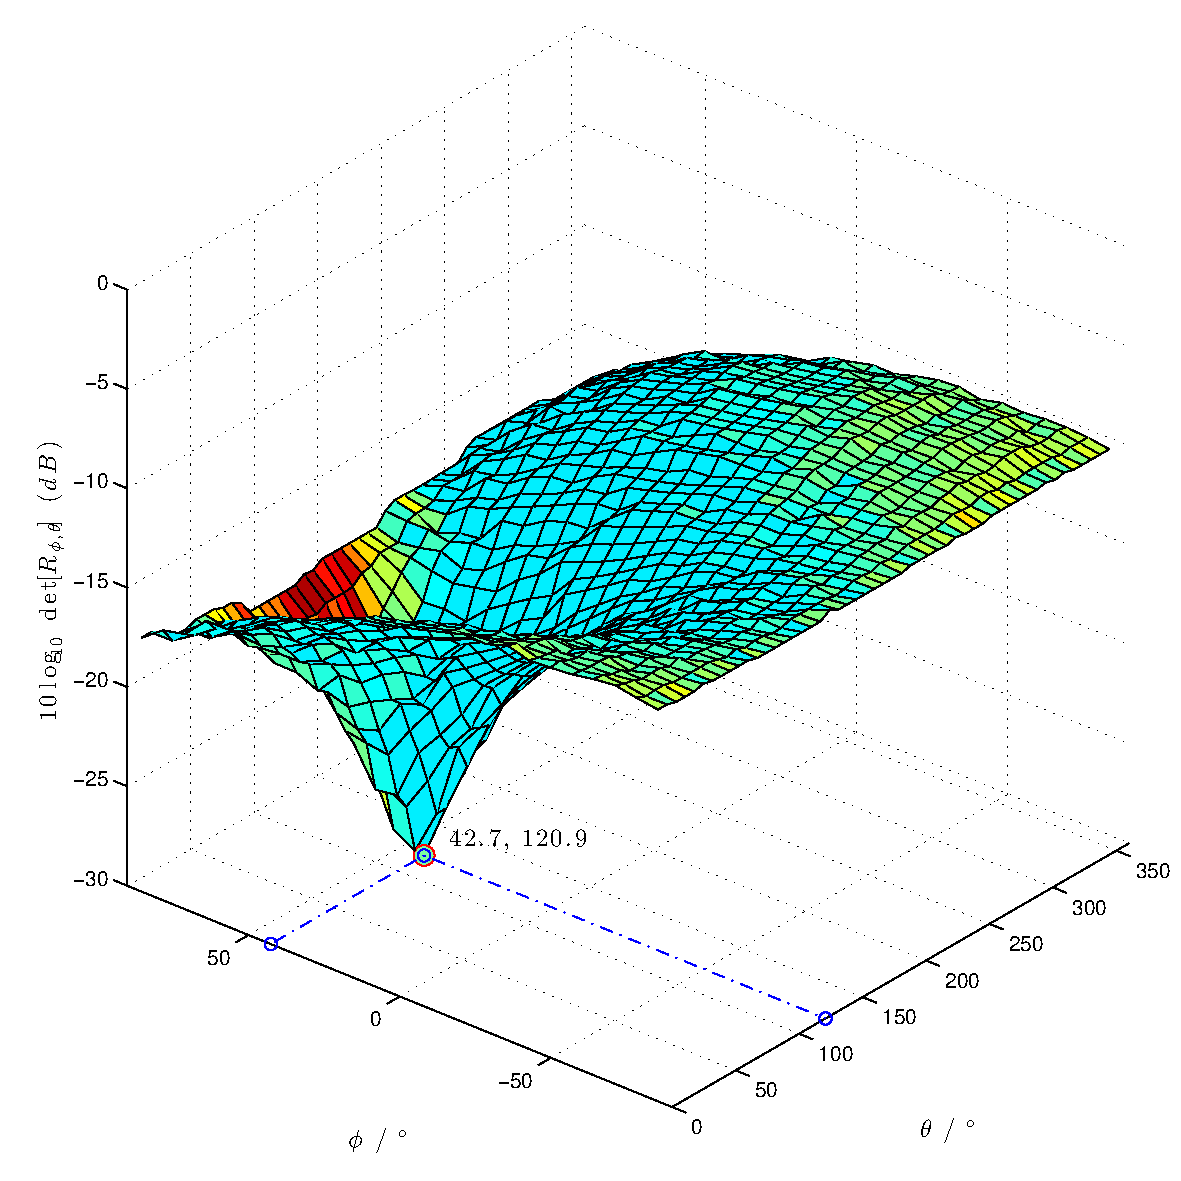
\includegraphics[width=\textwidth]{images/02_Konzeptionierung/Sim_sine_f_100_Phi_45_Theta_120_dB_SNR_100dB}
                \caption{$f=100Hz$}
                \label{fig:Sim_sine_f_100_Phi_45_Theta_120_dB_SNR_100dB}
        \end{subfigure}
        ~ %add desired spacing between images, e. g. ~, \quad, \qquad etc.
          %(or a blank line to force the subfigure onto a new line)
        \begin{subfigure}[b]{0.48\textwidth}
                \centering
                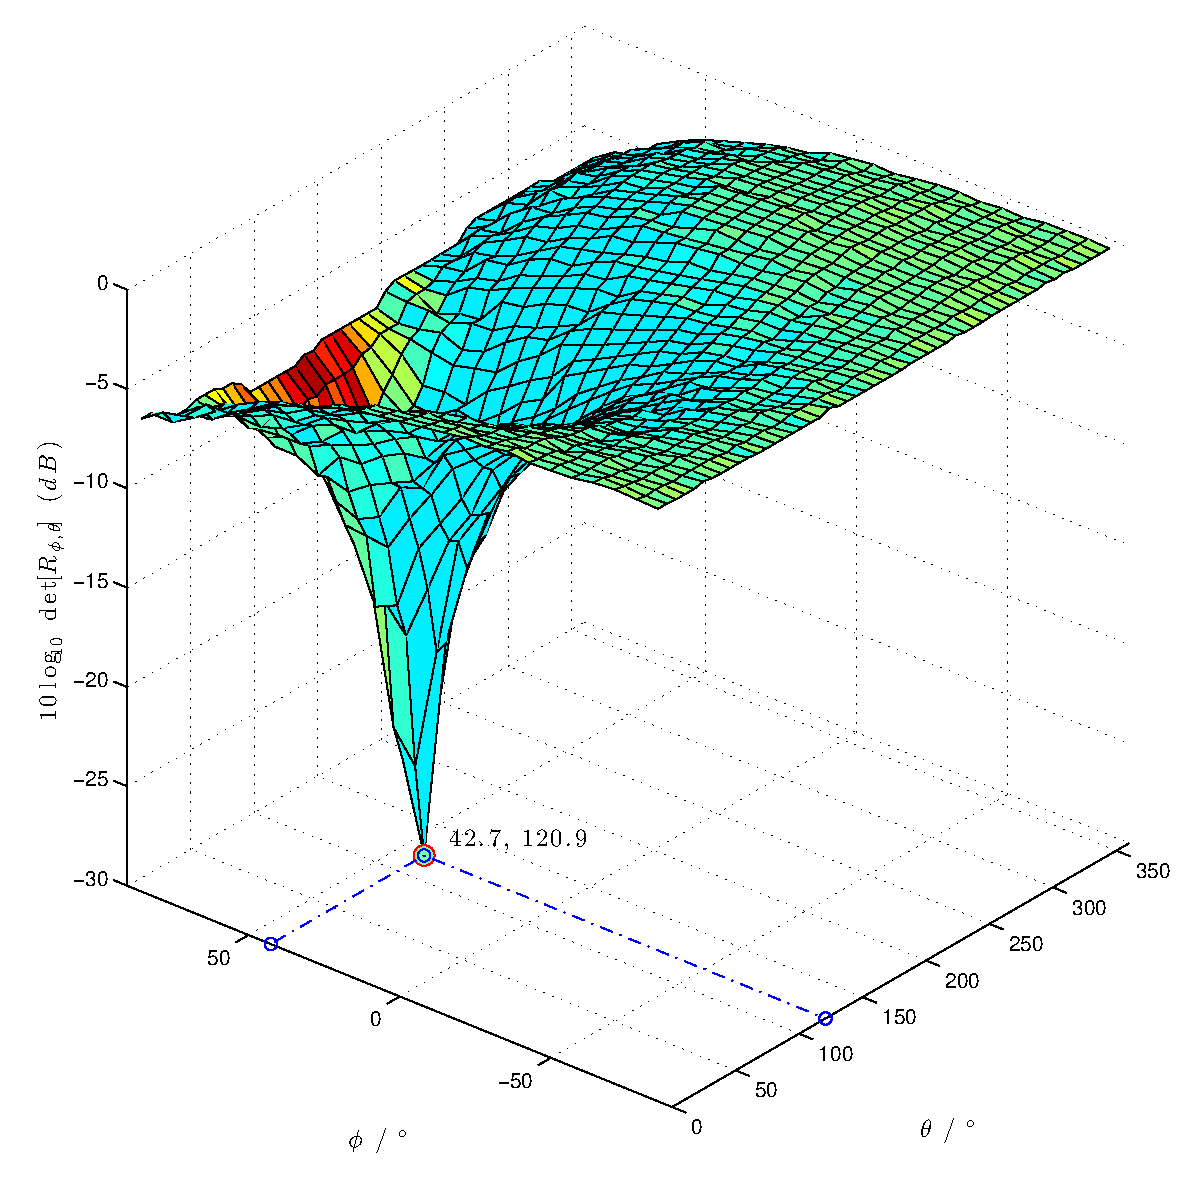
\includegraphics[width=\textwidth]{images/02_Konzeptionierung/Sim_sine_f_500_Phi_45_Theta_120_dB_SNR_100dB}
                \caption{$f=500Hz$}
                \label{fig:Sim_sine_f_500_Phi_45_Theta_120_dB_SNR_100dB}
        \end{subfigure}
        ~ %add desired spacing between images, e. g. ~, \quad, \qquad etc.
          %(or a blank line to force the subfigure onto a new line)
        \begin{subfigure}[b]{0.48\textwidth}
                \centering
                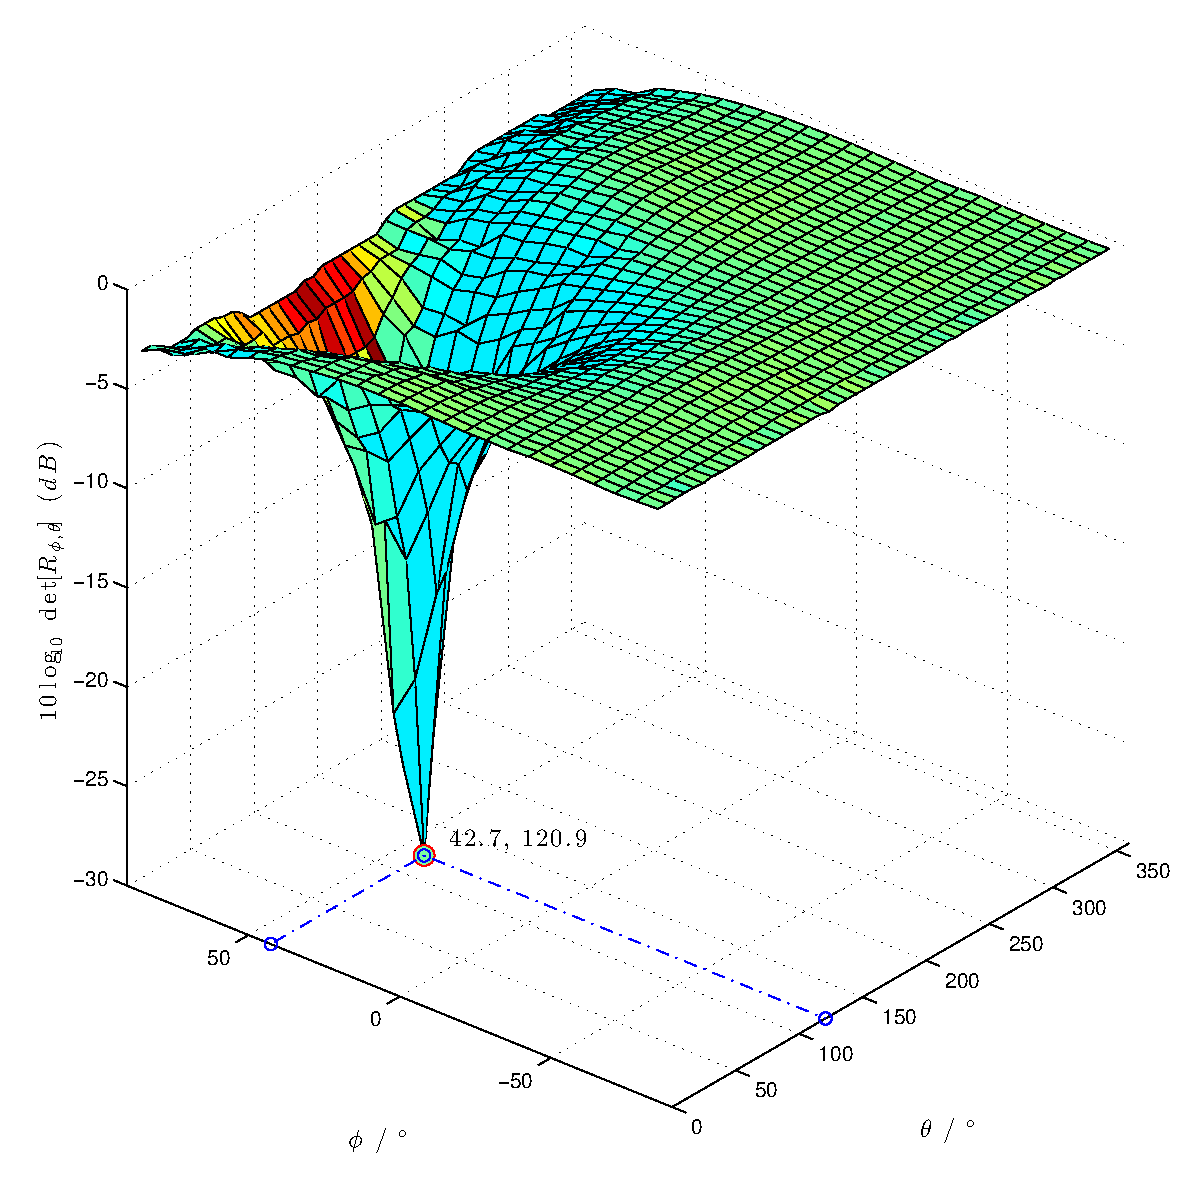
\includegraphics[width=\textwidth]{images/02_Konzeptionierung/Sim_sine_f_1000_Phi_45_Theta_120_dB_SNR_100dB}
                \caption{$f=1000Hz$}
                \label{fig:Sim_sine_f_1000_Phi_45_Theta_120_dB_SNR_100dB}
        \end{subfigure}
        ~ %add desired spacing between images, e. g. ~, \quad, \qquad etc.
          %(or a blank line to force the subfigure onto a new line)
        \begin{subfigure}[b]{0.48\textwidth}
                \centering
                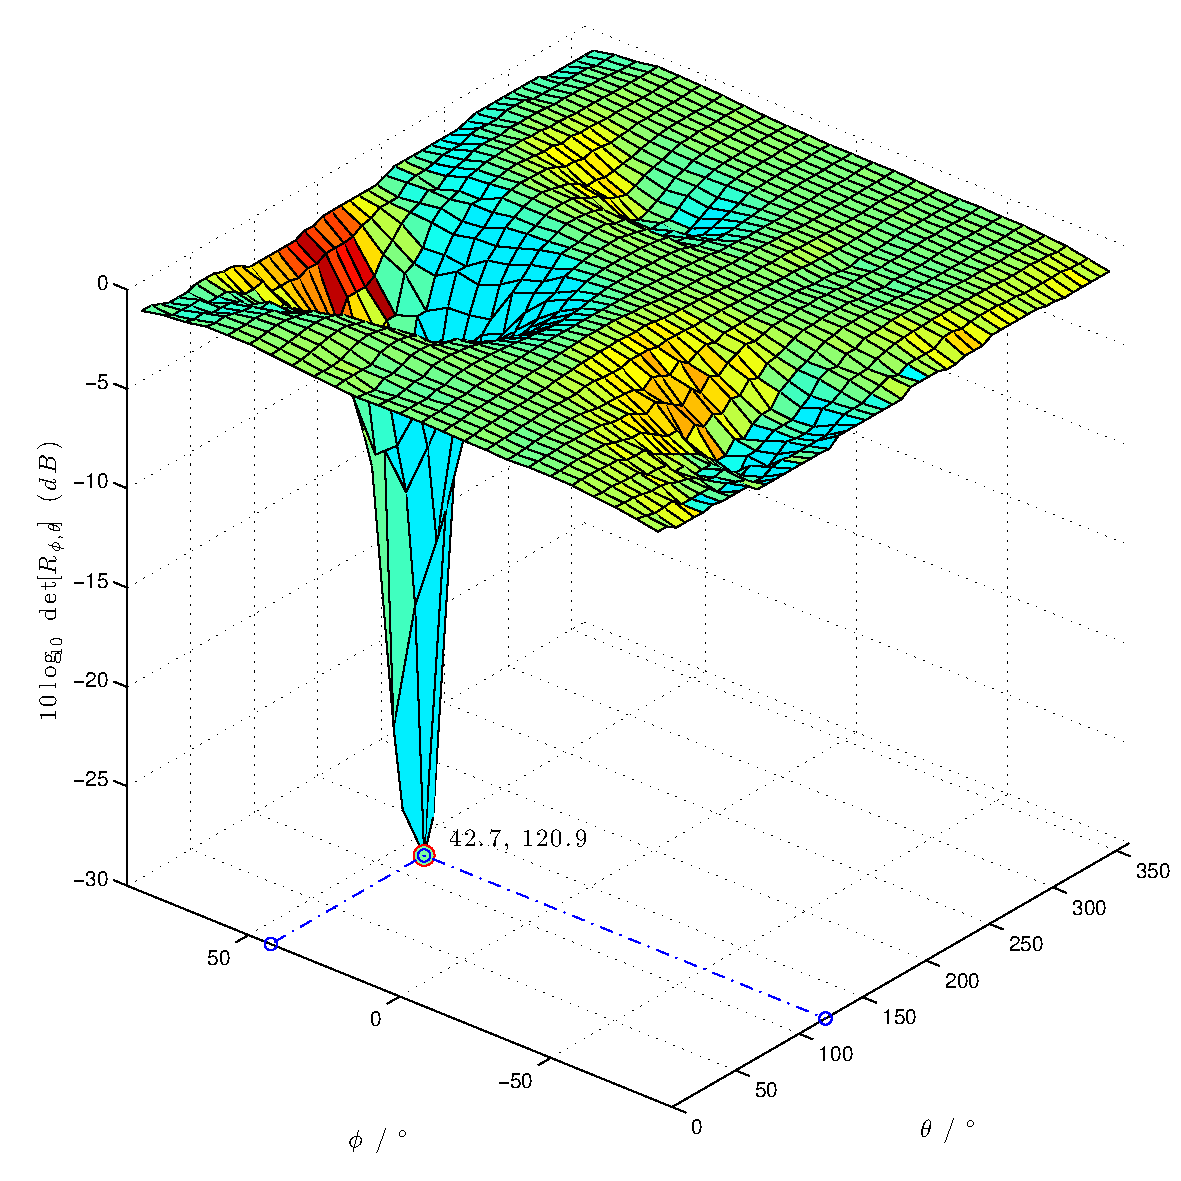
\includegraphics[width=\textwidth]{images/02_Konzeptionierung/Sim_sine_f_1500_Phi_45_Theta_120_dB_SNR_100dB}
                \caption{$f=1500Hz$}
                \label{fig:Sim_sine_f_1500_Phi_45_Theta_120_dB_SNR_100dB}
        \end{subfigure}
                ~ %add desired spacing between images, e. g. ~, \quad, \qquad etc.
          %(or a blank line to force the subfigure onto a new line)
        \begin{subfigure}[b]{0.48\textwidth}
                \centering
                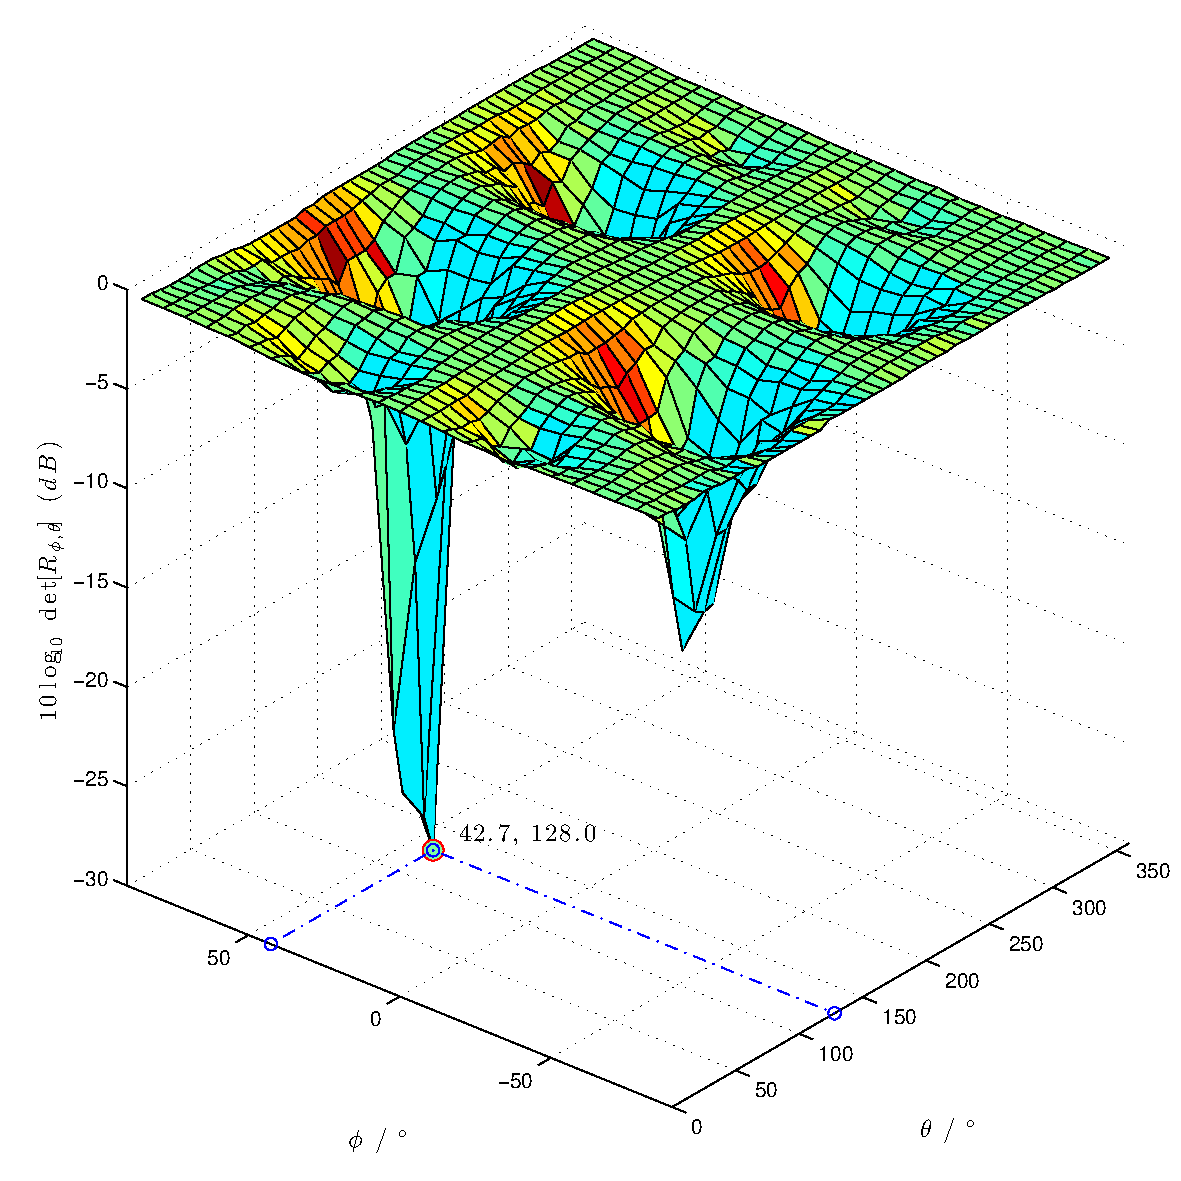
\includegraphics[width=\textwidth]{images/02_Konzeptionierung/Sim_sine_f_2000_Phi_45_Theta_120_dB_SNR_100dB}
                \caption{$f=2000Hz$}
                \label{fig:Sim_sine_f_2000_Phi_45_Theta_120_dB_SNR_100dB}
        \end{subfigure}
        ~ %add desired spacing between images, e. g. ~, \quad, \qquad etc.
          %(or a blank line to force the subfigure onto a new line)
        \begin{subfigure}[b]{0.48\textwidth}
                \centering
                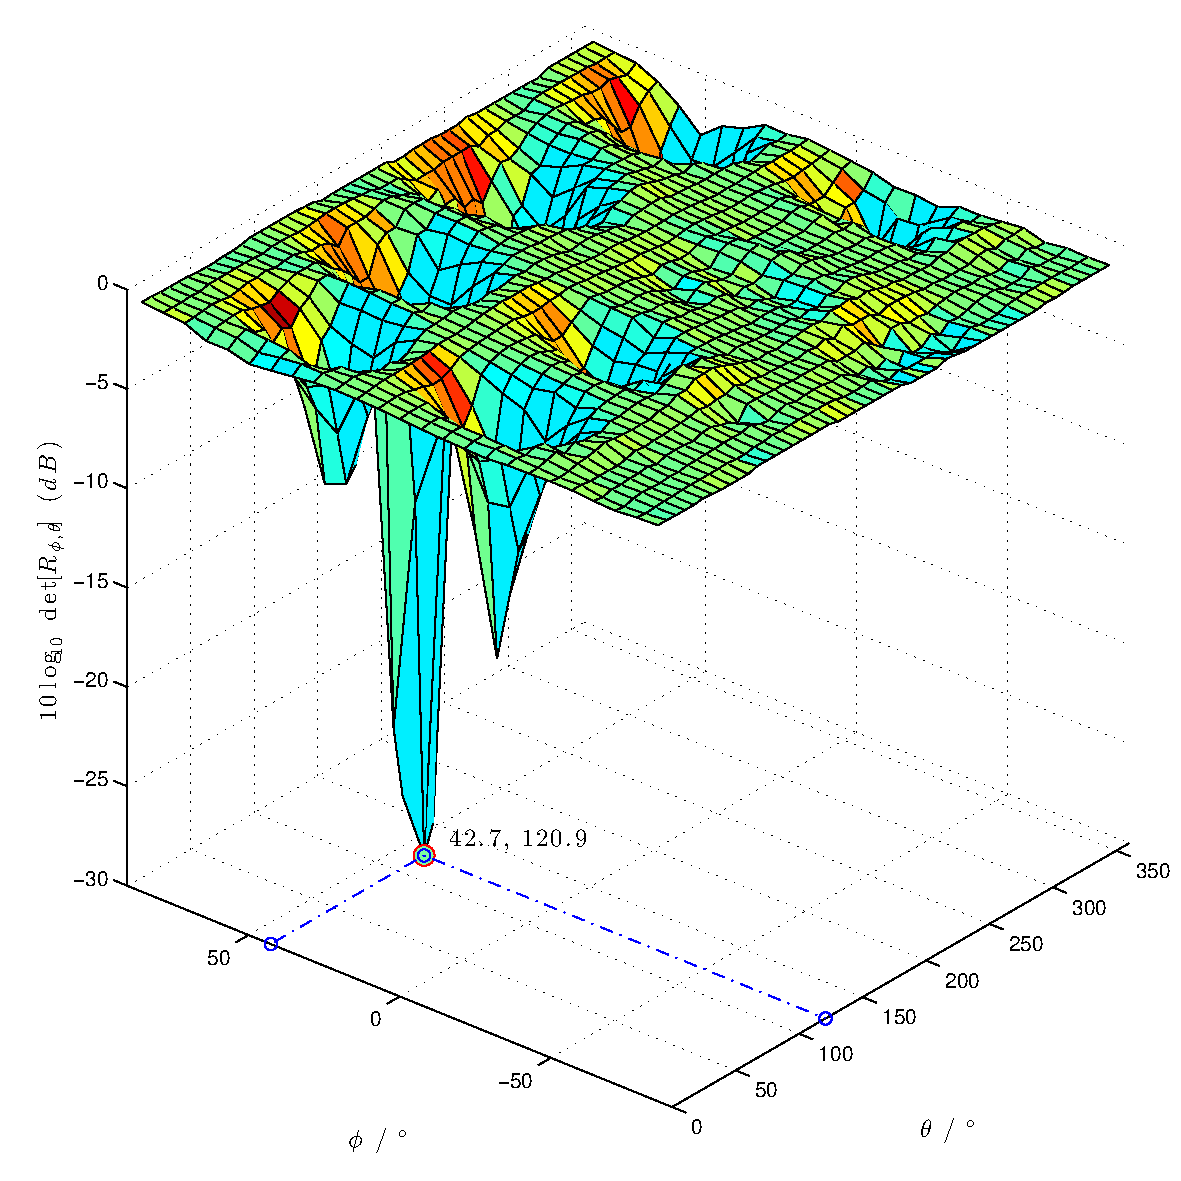
\includegraphics[width=\textwidth]{images/02_Konzeptionierung/Sim_sine_f_3000_Phi_45_Theta_120_dB_SNR_100dB}
                \caption{$f=3000Hz$}
                \label{fig:Sim_sine_f_3000_Phi_45_Theta_120_dB_SNR_100dB}
        \end{subfigure}
        \caption{Ergebnis des MCCC unter Verwendung eines synthetisch verzögerten periodischen Signals der Form $y(n) = \sin{\left( 2 \pi \frac{f}{f_a} n \right)}$ bei einer Abtastfrequenz von $f_a=48kHz$.}
        \label{fig:Sim_sine_spartial_aliasing}
\end{figure}
% ----------------------------------------- SUB-FIGURE -----------------------------------        
    


 % ****************************************************************************************
\subsubsection{Bewegte Sprachquelle} 
% ****************************************************************************************
Um das Verhalten des Systems auf eine sich durch den Raum bewegende Sprachquelle zu untersuchen, werden synthetischs Signale aus zwei folgendenSignaltypen erstellt:

\begin{itemize}
    \item bandbegrenztes weißes Rauschen
    \item Sprache (männlich und weiblich)
\end{itemize}

Folgende Simulationsparameter wurden verwendet:

\begin{itemize}
    \item Anzahl der Mikrofone $N=8$
    \item Abtastfrequenz $f_a = 44,1kHz$
    \item Signalblocklänge $L=256$ (Frame)
    \item FFT-Länge $K = 2 \cdot L = 512$
    \item Winkelauflösung $\alpha_{\phi, \theta} = 7,7°$ 
\end{itemize}

\abb{sim_diag_3D} zeigt einen künstlichen reflexionsfreien Raum mit den Abmaßen $5m \times 5m \times 3m$, in dessen Zentrum das Mikrofonarray positioniert ist. Die Rauschquelle bewegt sich hier diagonal und nimmt dabei Winkel im Bereich von $-90° \leq \phi \leq 90°$ und $\theta \in \{45°,225°\}$ an. In diesem Versuch werden zunächst die vier Eckpunkte platziert und anschließend mit einer Anzahl von 81 Stützstellen linear interpoliert. Die Rauschquelle bewegt sich somit entlang der Stützstellen um eine kleine Winkelschrittweite zu realisieren. \abb{sim_noise_diag} zeigt das Ergebnis dieses Simulationsdurchlaufs. Die in rot abgebildete Linie stellt den Fehler zu den tatsächlich eingenommene Winkeln dar. Alle Signalblöcke mit einer Blockenergie von weniger als der eingezeichneten Schwelle werden mit einem Wert $0°$ detektiert. Da wie bereits erwähnt nur diskrete Werte eingenommen werden können ist ein Fehler von $\pm \frac{\alpha_{\phi, \theta}}{2}$ zu tolerieren. Beim Betrachten des Azimuthwinkelverlaufs fällt auf, dass an den Stellen, an denen der Elevationswinkel $\phi=90°$ einnimmt ein plötzlicher Fehleranstieg stattfindet. Der Grund hierfür ist, dass sich die Quelle genau im oberen Winkeltotpunkt befindet und eine Drehung auf den Azimuthwinkel nicht erkannt werden kann. 




\myFigure{real}                                                   % Figure tag (missing, real)
         {big}                                                       % Size (small,medium,big)
         {h!}                                                  % z.B. htbp
         {Wegstrecke einer Rauschquelle  die sich diagonal durch den Raum bewegt}    % Figure title
         {sim_diag_3D}                                               % Figure label 
         {02_Konzeptionierung/sim_diag_3D}  




\myFigure{real}                                                   % Figure tag (missing, real)
         {max}                                                       % Size (small,medium,big)
         {h!}                                                  % z.B. htbp
         {Simulationsergebnis einer Rauschquelle  bei einer Blockenergieschwelle von -10dB.}    % Figure title
         {sim_noise_diag}                                               % Figure label 
         {02_Konzeptionierung/sim_noise_diag_errorbar}   



Im Folgenden soll nun eine bewegte Sprachquelle simuliert werden. Wie in \abb{sim_zig_zag_3D} dargestellt, bewegt sie sich sägezahnförmig um das Mikrofonarray und nimmt dabei Winkel im Bereich von $-45° \leq \phi \leq 45°$ und $0° \leq \theta < 360°$ an. Als Grundlage wird eine Audiodatei der Länge $T_{file}=16s$ verwendet. Bei einem zurückgelegten Weg von $s=28,9m$ beträgt die Durchschnittsgeschwindigkeit der Quelle $v=\frac{s}{T_{file}} = 6,5 \frac{km}{h}$ was der allgemeinen Angabe zur Schrittgeschwindigkeit nahe kommt.
\abb{sim_male_zig_zag} und \abb{sim_female_zig_zag} illustrieren die Ergebnisse der beiden Simulationsdurchläufe. Zu beachten ist, dass die Signale synthetisch mit dem in \Sec{subsec:ErstellungSynthetischerSignale} beschriebenen Verfahren (ohne Reflexion) blockweise verzögert werden. Die Phasenverschiebung zwischen den Kanälen ändert sich somit sprunghaft und nicht kontinuierlich wie in realer Umgebung. Die fehlerhaft erkannten Winkel (Winkelsprünge) sind zum großen Teil auf diese plötzliche Phasenänderung zurückzuführen. Die in rot abgebildete Linie stellt die Referenz zu den tatsächlich eingenommenen Winkeln dar. Alle Signalblöcke mit einer Blockenergie von weniger als der in rot dargestellten Schwelle werden mit dem Wert $0°$ detektiert. Beim Vergleich der beiden Ergebnisse zeigt sich, dass  die Zuverlässigkeit der Winkelerkennung deutlich voneinander abweicht. Dies lässt sich zum einen durch das unterschiedliche Frequenzspektrum zwischen männlicher und weiblicher Sprache begründen, zum anderen liegt eine große Differenz im Dynamikbereich\footnote{Bereich zwischen größter und kleinster Signalstärke} vor. Im Vergleich zur weiblichen Sprecherin ist der männliche etwa doppelt so groß. Die Blockenergieschwelle wird für die Simulation abhängig vom Dynamikbereich etwa in dessen Mittel gelegt. Die Ergebnisse erweisen sich trotz gelegentlicher Winkelsprünge als zufriedenstellend da die Bewegung der Quelle gut verfolgbar ist.



\myFigure{real}                                                   % Figure tag (missing, real)
         {big}                                                       % Size (small,medium,big)
         {h!}                                                  % z.B. htbp
         {Wegstrecke einer männlichen Sprechquelle die sich Zig-Zag-förmig von Position 1 bis 9 um das Mikrofonarray bewegt.}    % Figure title
         {sim_zig_zag_3D}                                               % Figure label 
         {02_Konzeptionierung/sim_zig_zag_3D}    




\myFigure{real}                                                   % Figure tag (missing, real)
         {max}                                                       % Size (small,medium,big)
         {h!}                                                  % z.B. htbp
         {Simulationsergebnis eines bewegten männlichen Sprechers (deutschsprachig) bei einer Blockenergieschwelle von -30dB.}    % Figure title
         {sim_male_zig_zag}                                               % Figure label 
         {02_Konzeptionierung/sim_male_zig_zag}    


\myFigure{real}                                                   % Figure tag (missing, real)
         {max}                                                       % Size (small,medium,big)
         {h!}                                                  % z.B. htbp
         {Simulationsergebnis eines bewegten weiblichen Sprechers (englischsprachig) bei einer Blockenergieschwelle von -20dB.}    % Figure title
         {sim_female_zig_zag}                                               % Figure label 
         {02_Konzeptionierung/sim_female_zig_zag}    







%\subsubsection{Reale Signale}





                  
% ****************************************************************************************         
\subsection{Optimierungsverfahren}
\label{subsec:Optimierungsverfahren}
% ****************************************************************************************
Im Hinblick auf die spätere Echtzeitimplementierung auf einem DSP gilt es, den Rechenaufwand so gering wie möglich zu halten. Auf Grund dessen wird ein Verfahren zur Optimierung der Suchgeschwindigkeit entwickelt. Als zweiter Optimierungsschritt folgt eine Histogrammschätzung der Richtungsergebnisse. Dieser vermindert den Effekt der abrupten Winkelsprünge. 

% ****************************************************************************************
\subsubsection{Suchgeschwindigkeit}
\label{subsubsec:Suchgeschwindigkeit}
% ****************************************************************************************
Zur Verbesserung der Suchgeschwindigkeit wird eine Methode entwickelt, die sich mit Hilfe von variablen Schrittweiten sukzessive an den korrekten Winkel annähert. \abb{prinzip_opt_suchgeschwindigkeit} zeigt das zu Grunde liegende Prinzip. Der abzusuchende Winkelbereich wird zunächst in drei Gebiete geteilt. Nun wird an den Bereichsübergängen nach dem Minimum in der räumlichen Korrelationsmatrix $R_{\phi, \theta}$ gesucht. Der gefundenen Winkel wird in der nächsten Itteration als neuer Starpunkt gewählt. Anschließend erfolgt eine Halbierung des Suchbereiches und der Vorgang beginnt erneut. Dieser Algorithmus wird so lange wiederholt, bis die minimale Schrittweite erreicht wurde. 

\myFigure{real}                                                   % Figure tag (missing, real)
         {medium}                                                       % Size (small,medium,big)
         {h!}                                                  % z.B. htbp
         {Methode zur Optimierung der Suchgeschwindigkeit mit Hilfe einer variablen Schrittweiten.}    % Figure title
         {prinzip_opt_suchgeschwindigkeit}                                               % Figure label 
         {02_Konzeptionierung/prinzip_opt_suchgeschwindigkeit} 


% ****************************************************************************************
\subsubsection{Histogramm}
\label{subsubsec:Histogramm}
% ****************************************************************************************
Zur Reduktion der Winkelsprünge bei \zB überlagerten Störungen wird im Folgenden eine Histogrammschätzung durchgeführt. Die detektierten Winkel werden im laufenden Betrieb kontinuierlich in einen Ringspeicher mit einer variabel einstellbaren Länge gespeichert. Nach jedem Suchvorgang erfolgt eine Häufigkeitsanalyse des Ringspeicherinhalts. \abb{sim_female_zig_zag_dist_sample_frame_864} zeigt illustriert ein Beispiel für die Häufigkeitsanalyse des weiblichen Sprachsignals mit einer Ringspeicherlänge von 50 Werten sowie einer Häufigkeitsschwelle von 20\%. Tritt ein gemessener Winkel so häufig auf, dass er diese Schwelle überschreitet wird er als wahrscheinlich genug eingestuft und als gültig markiert. Tritt der Fall ein, dass die Häufigkeit keines Ringspeicherwerts diese Schwelle überschreitet, markiert der Algorithmus den aktuellen Signalblock als ungültig.



\abb{sim_male_female_zig_zag_hist_comp} und \abb{sim_male_zig_zag_hist_comp} zeigen einen Vergleich der Simmulationsergebnisse des männlichen und weiblichen Sprechers mit und ohne Histogrammoptimierung. Es ist deutlich zu sehen, dass abrupte Winkelsprünge nahezu verschwiden. Bei solch einem Verfahren, das Ergebniswerte zwischenspeichert, tritt eine Verzögerung auf, die abhängig von der Ringspeicherlänge sowie der eben erwähnten Schwelle ist. Im Vergleich zum nicht optimierten Ergebnis ist das optimierte leicht zur Winkelreferenzkurve verschoben.


\myFigure{real}                                                   % Figure tag (missing, real)
         {medium}                                                       % Size (small,medium,big)
         {h!}                                                  % z.B. htbp
         {Histogramm eines bewegten weiblichen Sprechers}    % Figure title
         {sim_female_zig_zag_dist_sample_frame_864}                                               % Figure label 
         {02_Konzeptionierung/sim_female_zig_zag_dist_sample_frame_864} 


\myFigure{real}                                                   % Figure tag (missing, real)
         {max}                                                       % Size (small,medium,big)
         {h!}                                                  % z.B. htbp
         {Vergleich zwischen Winkelverlauf mit und ohne Histogrammschätzung beim weiblichen Sprecher mit einer Ringspeicherlänge von 50 und einer Schwelle von 15\%}    % Figure title
         {sim_male_female_zig_zag_hist_comp}                                               % Figure label 
         {02_Konzeptionierung/sim_female_zig_zag_hist_comp} 


\myFigure{real}                                                   % Figure tag (missing, real)
         {max}                                                       % Size (small,medium,big)
         {h!}                                                  % z.B. htbp
         {Vergleich zwischen Winkelverlauf mit und ohne Histogrammschätzung beim männlichen Sprecher mit einer Ringspeicherlänge von 50 und einer Schwelle von 15\%}    % Figure title
         {sim_male_zig_zag_hist_comp}                                               % Figure label 
         {02_Konzeptionierung/sim_male_zig_zag_hist_comp} 







	% ****************************************************************************************
\chapter{Realisierung}
\label{chap:Realisierung}
% ****************************************************************************************
In diesem Kapitel folgt die Beschreibung der Realisierung des im \Chap{Konzeptionierung} vorgestellten Systemkonzepts. Zunächst werden, die Hardware sowie die damit verbundenen Einschränkungen im Vergleich zur Simulation in \matlab erläutert. Anschließend erfolgt die Darstellung der Programmumsetzung mit der Programmiersprache C.  


% ****************************************************************************************
%\section{Implementierung als Echtzeitsystem}
%\label{Sec:ImplementierungAlsEchtzeitsystem}
% ****************************************************************************************
%Zur Implementierung des 3D-Tracking-Algorithmus ist eine Hardware notwendig die über ausreichen Peripherie zum Anschluss der nötigen Anzahl von Mikrofonen verfügt sowie über genügend Rechenleistung um alle Rechenschritte in der vorgegebenen Zeit (siehe \tab{Systemparameter}) durchführen kann. 


% ****************************************************************************************
\section{Verwendete Hardware}
\label{sec:VerwendeteHardware}
% ****************************************************************************************
Zur Implementierung des 3D-Tracking-Algorithmus ist eine Hardware notwendig, die über ausreichend Peripherie zum Anschluss der nötigen Anzahl von Mikrofonen verfügt sowie über genügend Rechenleistung um alle Rechenschritte in der vorgegebenen Zeit (siehe \tab{Systemparameter}) durchführen zu können.

\abb{blockdiagramm_used_hardware} zeigt eine detaillierte schematische Darstellung der verwendeten Systemkomponenten. Diese gliedern sich in drei Kategorien, die im Folgenden vorgestellt werden.

\begin{enumerate}
    \item Schallwandler Front-End
    \item DSP Back-End
    \item Display (PC)
\end{enumerate}


\myFigure{real}                                                   % Figure tag (missing, real)
         {max}                                                       % Size (small,medium,big)
         {h!}                                                  % z.B. htbp
         {Blockdiagramm der verwendeten Hardware}    % Figure title
         {blockdiagramm_used_hardware}                                               % Figure label 
         {03_Realisierung/blockdiagramm_used_hardware} 


% ****************************************************************************************
\subsection{Schallwandler Front-End}
\label{subsec:SchallwandlerFrontEnd}
% ****************************************************************************************
Die erste Stufe des Echtzeitsystems beinhaltet das Mikrofonarray (siehe \abb{Vergleich_array_gefertigt}), das die akustischen in elektrische Signale wandelt. Bei den Schallwandlern handelt es sich um omnidirektionale\footnote{Druckempfänger mit einer Kugelcharakteristik} Kondensatormikrofone der Firma \sennheiser. Auf Grund des niedrigen Signalpegels, den ein Mikrofon ausgibt, muss eine Verstärkungsstufe zwischen Array und ADC\footnote{Analog/Digital-Converter} geschaltet werden. Um die Bittiefe des Wandlers vollständig ausnutzen zu können gilt es, das Mikrofonsignal bis auf eine Spannung von 1,8Vpp\footnote{Spitze-Spitze-Wert} zu verstärken. \abb{Mikrofonverstaerker} zeigt den Stromlaufplan der Verstärkerschaltung. Als Basiskomponente wird ein Operationsverstärker eingesetzt, der als nicht-invertierter OPV beschaltet ist. Wie in \abb{Mikrofonverstaerker} ersichtlich wird ein Teil der Betriebsspannung auf den Signaleingang gekoppelt. Grund hierfür ist, dass das Eingangssignal während der Aufnahme positive sowie negative Werte annehmen kann. Da lediglich eine positive Betriebsspannung zur Verfügung stehet, ist der OPV nur in der Lage, den Wert der Betriebsspannung als Maximalwert und den Wert Null als Minimalwert anzunehmen. Die auf den Signaleingang gekoppelte Gleichspannung wirkt hier wie ein Offset um den Signalruhepegel in die Mitte des zur Verfügung stehenden Spannungsbereiches zu verschieben. Auf Grund dessen lassen sich positive sowie negative Signalverläufe verstärken und so optimal auf den Spannungsbereich des ADC abstimmen.

\myFigure{real}                                                   % Figure tag (missing, real)
         {Big}                                                       % Size (small,medium,big)
         {h!}                                                  % z.B. htbp
         {Stromlaufplan des Mikrofonvorverstärkers für einen Kanal}    % Figure title
         {Mikrofonverstaerker}                                               % Figure label 
         {03_Realisierung/Mikrofonverstaerker} 


% ****************************************************************************************
\subsection{DSP Back-End}
% ****************************************************************************************
Wie in \abb{blockdiagramm_used_hardware} dargestellt, besteht die zweite Signalverarbeitungsstufe aus der I/O\footnote{Input/Output}-Flachbaugruppe D.Module.PCM3003 sowie aus der DSP-Flachbaugruppe D.Module.C6713 der Firma D.SignT und bildet so das DSP Back-End. \abb{DSP_PCM3003} zeigt beide Module im Zusammenbau mit jeweils acht Anschlüssen für ADC/DAC-Module.


% ----------------------------------------- SUB-FIGURE -----------------------------------
\begin{figure}
        \centering
        \begin{subfigure}[b]{0.48\textwidth}
                \centering
                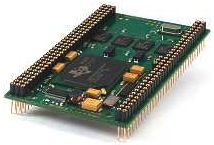
\includegraphics[width=\textwidth]{grafiken/03_Realisierung/DSP6713}
                \caption{D.Module.C6713}
                \label{fig:D.Module.C6713}
        \end{subfigure}
        ~ %add desired spacing between images, e. g. ~, \quad, \qquad etc.
          %(or a blank line to force the subfigure onto a new line)
        \begin{subfigure}[b]{0.48\textwidth}
                \centering
                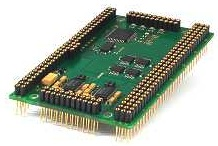
\includegraphics[width=\textwidth]{grafiken/03_Realisierung/PCM3003}
                \caption{D.Module.PCM3003}
                \label{fig:D.Module.PCM3003}
        \end{subfigure}
        \caption{DSP-Flachbaugruppe D.Module.C6713 und A/D-Wandler D.Module.PCM3003}
        \label{fig:DSP_PCM3003}
\end{figure}
% ----------------------------------------- SUB-FIGURE -----------------------------------


Das D.Module.PCM3003 Modul ist ein Audiocodec, der speziell für Mehrkanal-Audio Signalverarbeitung sowie Mikrofonarrayverarbeitung designed wurde \cite[S. 1]{Manual_PCM3003}. \abb{PCM3003_blockdiagramm} zeigt alle Funktionsblöcke in einem Blockdiagramm. Der Codec verfügt über vier Stereo-ADC/DAC Module und kann so im Vierkanal-Stereo-Mode oder im Achtkanal-Mono-Mode betrieben werden. Da in dieser Arbeit acht Mikrofonsignale simultan verarbeitet werden sollen, wird der Achtkanal-Mono-Mode gewählt. Jedes der vier ADC/DAC-Module besitzt eine Auflösung von 16 bit und einen Delta-Sigma-Modulator 64. Ordnung. Alle ADC/DAC-Sektionen werden synchrone von einem einstellbaren Oszillator getaktet und können auf die im Audiobereich gängigen Abtastraten konfiguriert werden. Die Übertragung der Abtastwerte an den DSP erfolgt über zwei serielle Schnittstellen wobei jeweils zwei ADC/DAC-Stufen zu einer Schnittstelle führen. Alle notwendigen Synchronisationssignale werden von diesem Modul erzeugt, so dass es als Mastergerät fungiert.


\myFigure{real}                                                   % Figure tag (missing, real)
         {big}                                                       % Size (small,medium,big)
         {h!}                                                  % z.B. htbp
         {Blockdiagramm des D.SignT Moduls D.Module.PCM3003 (\vgl \cite[S. 1]{Manual_PCM3003})}    % Figure title
         {PCM3003_blockdiagramm}                                               % Figure label 
         {03_Realisierung/PCM3003_blockdiagramm} 



Das D.Module.C6713 Modul ist eine DSP Flachbaugruppe, dessen CPU\footnote{Central processing unit} der von \ti entwickelte TMS320C6713b aus der Prozessorreihe TMS320C6000 ist. Dieser DSP basiert 
auf einer Very Long Instruction Word Architektur mit einer Wortbreite von 256 bit und ist so in der Lange, bis zu acht 32-bit Befehle für jeweils einen der acht Funktionseinheiten innerhalb eines Taktschrittes zu verarbeiten \cite[S. 14]{Manual_dsp_datasheet}. Weiterhin kann der TMS320C6713b sowohl in Festkomma- als auch in Fließkomma-Arithmetik programmiert werden und unterstützt einen Prozessortakt von bis zu 300MHz wodurch eine Rechengeschwindigkeit von 1,8 GFLOPS\footnote{Giga-floating-point operations per second} erreicht werden kann. \abb{dsp_core_blockdiagramm} zeigt das Blockdiagramm mit der zur Verfügung stehenden Peripherie. Als Schnittstellen stehen unter anderem zwei Multi-channel-Buffered Serial Port (McBSP) und ein I2C Interface zur Verfügung, die mit Hilfe eines Enhanced Direct Memory Access (EDMA) Controller mit dem internen Speicher verknüpft sind. Die DSP-Flachbaugruppe bietet darüber hinaus noch folgende Funktionen:

\begin{itemize}
    \item 64 MB SDRAM\footnote{Synchronous Dynamic Random Access Memory} mit 100MHz Taktfrequenz
    \item 2MB Flash Speicher
    \item 256 kB Interner Speicher (für Programmcode sowie vom Programm benötigter Speicher)
    \item USB Schnittstelle zum PC inkl. JTAG\footnote{Joint Test Action Group} Emulator
    \item LED's sowie Taster zur Benutzerinteraktion
\end{itemize}


Als Programmierwerkzeug wird die von \ti entwickelte Softwarelösung \ccs verwendet.
Dieses Eclips-basierte Softwarepaket beinhaltet einen Sourcecode-Editor, eine Projektumgebung, eine Debug-Umgebung sowie die Möglichkeit Variable im laufenden Betrieb zu observieren und Speicherinhalte grafisch darzustellen. \ccs verfügt über einen C-Compiler, einen Assembler sowie einen Linker und wird in dieser Arbeit in Version 5 verwendet.


\myFigure{real}                                                   % Figure tag (missing, real)
         {max}                                                       % Size (small,medium,big)
         {h!}                                                  % z.B. htbp
         {Blockdiagramm des D.SignT DSP D.Module.C6713 (\vgl \cite[S. 1]{Manual_C6713})}    % Figure title
         {C6713_blockdiagramm}                                               % Figure label 
         {03_Realisierung/C6713_blockdiagramm} 



\myFigure{real}                                                   % Figure tag (missing, real)
         {max}                                                       % Size (small,medium,big)
         {h!}                                                  % z.B. htbp
         {Blockdiagramm der TMS320C6713b CPU (\vgl \cite[S. 13]{Manual_dsp_datasheet})}    % Figure title
         {dsp_core_blockdiagramm}                                               % Figure label 
         {03_Realisierung/dsp_core_blockdiagramm} 




% ****************************************************************************************
\subsection{Kommunikationsschnittstelle zwischen DSP und PCM3003}
\label{subsec:Kommunikationsschnittstelle_DSP_PCM3003}
% ****************************************************************************************
Als Kommunikationsschnittstelle zwischen DSP und PCM3003 dienen die vom DSP bereitgestellten McBSP. Der Datenaustausch findet so jeweils über zwei Datenleitungen statt, wobei eine die eingehenden und die andere die ausgehenden Daten enthält. Steuersignale wie Synchronisation und Taktung werden über eine separate Leitung übertragen. \abb{McBSP_blockdiagramm} illustriert das Funktionsblockdiagramm eines McBSP Moduls. Eine detaillierte Erklärung zu den Funktionen der einzelnen Pins und Register befindet sich in \cite{Manual_McBSP_Report}.
Die Übertragung der Daten in einem seriellen Datenstrom findet in einem speziellen Musterstatt wie in \tab{McBSP_Muster} dargestellt.


\myFigure{real}                                                   % Figure tag (missing, real)
         {small}                                                       % Size (small,medium,big)
         {h!}                                                  % z.B. htbp
         {McBSP Fubktionsblockdiagramm (\vgl \cite[S. 2]{Manual_McBSP_Report})}    % Figure title
         {McBSP_blockdiagramm}                                               % Figure label 
         {03_Realisierung/McBSP_blockdiagramm} 



Ein Muster dieser Art entsteht, da der PCM3003 die Ausgabedaten zweier ADC auf eine Datenleitung zusammenfasst (Multiplexing) und an den DSP versendet. Im Umkehrschluss findet eine Trennung der zusammengefassten Daten statt (Demultiplexing), wenn der DSP Daten an den PCM3003 überträgt. \abb{McBSP_reihenfolge} zeigt, in welcher Reihenfolge die Kanäle in die beiden Datenströme zusammengefasst werden \cite{Code_PCM3003Demo}. 

\begin{table}[h]
     \center
     \begin{tabular}{clc}
     \hline
          Codec & Kanal &  DSP-Kanal  \\
          \hline \hline
          1     & links      & 0      \\
          2     & links      & 2      \\
          1     & rechts     & 1      \\
          2     & rechts     & 3      \\
          3     & links      & 4      \\
          4     & links      & 6      \\
          3     & rechts     & 5      \\
          4     & rechts     & 7      \\
         \hline
     \end{tabular}
  \caption{McBSP Kanalzuordnung}
 \label{tab:McBSP_Muster}
 \end{table}




\myFigure{real}                                                   % Figure tag (missing, real)
         {big}                                                       % Size (small,medium,big)
         {h!}                                                  % z.B. htbp
         {Reihenfolge des Kanalmultilexing durch den McBSP}    % Figure title
         {McBSP_reihenfolge}                                               % Figure label 
         {03_Realisierung/McBSP_reihenfolge}


% ****************************************************************************************
\subsection{EDMA-Verfahren}
\label{subsec:EDMAVerfahren}
% ****************************************************************************************
Der herkömmliche Weg, Abtastwerte aus einem ADC-Register zu lesen, ist durch Verwendung einer Interrupt-getriggerten Funktion (ISR\footnote{Interrupt Service Routinen}). Dies bedeutet allerdings, dass der DSP im Intervall der Abtastfrequenz seine aktuelle Operation unterbrechen muss, um die ISR auszuführen. In Anbetracht eines echtzeitfähigen Systems, in dem alle Berechnungen innerhalb eines Signalblocks (besteht hier aus einer Anzahl von 256 Abtastwerten) erfolgen müssen sind Unterbrechungen solcher Art von großem Nachteil. 

Zur Vermeidung von Unterbrechungen ist es erforderlich, dass der Prozess der Datensammlung einem zusätzlichen Modul zugeteilt wird. Das System verwendet daher den EDMA-Controller zur Sammlung von Abtastwerten. Mit einer vorher definierten Blockgröße informiert der EDMA-Controller den DSP mit Hilfe eines Interrupt, wann ein Block bereit zur Datenverarbeitung ist. Des Interrupt-Intervall hängt nun von der Abtastfrequenz sowie der Blocklänge ab. Die Kommunikationsschritte zwischen DSP und EDMA-Controller lassen sich wie in \abb{EDMA_Interrupt} dargestellt chronologisch auflisten:

\begin{enumerate}
    \item Die Hauptroutine initialisiert alle nötigen EDMA-Register und startet diesen.
    \item Die Hauptroutine wartet auf den Interrupt vom EDMA-Contoller welcher signalisiert, dass ein Signalblock bereit zur Datenverarbeitung ist-
    \item Die Datenverarbeitung beginnt, sobald ein EDMA-Interrupt empfangen wurde.
    \item Nach Beenden der Datenverarbeitung wartet die Hauptroutine auf den nächsten EDMA-Interrupt.
\end{enumerate}


\myFigure{real}                                                   % Figure tag (missing, real)
         {big}                                                       % Size (small,medium,big)
         {h!}                                                  % z.B. htbp
         {Interrupthandling zwischen EDMA-Controller und der Hauptroutine}    % Figure title
         {EDMA_Interrupt}                                               % Figure label 
         {03_Realisierung/EDMA_Interrupt}



% ****************************************************************************************
\subsection{Ping-Pong-Speicherverfahren}
\label{subsec:PingPongSpeicherverfahren}
% ****************************************************************************************
Zur Vermeidung von Datenverlust während der Datenverarbeitung eines Signalblocks sowie die zur Schaffung einer Möglichkeit zur unkomplizierten Einstellung des Zeitverhalten der Datenverarbeitungsroutine wird im Folgenden ein Ping-Pong-Speicherverfahren (Doublebuffer) angewendet. Hierbei sind anstelle eines Speicherfeldes zwei Felder mit identischer Größe im Einsatz. Wie in \abb{ping_pong_verfahren} dargestellt, alterniert die Datenverarbeitung zwischen diesen beiden Speichern. Vorteil dieser Methode ist, dass während der Verarbeitung eines Datenblocks im Hintergrund (nebenläufig) der zweite Block mit neuen Daten beschrieben wird. So kommt es bei den kontinuerlich am Mikrofonarray eintreffenden Audiosignalen zu keinem Datenverlust. Weiterhin entsteht so eine definierter Zeitabschnitt, in dem der Algorithmus seine Berechnungen abgeschlossen haben muss. Die wesentlichen Schritte dieses Verfahrens lassen sich wie folgt auflisten:


\begin{enumerate}
    \item Der EDMA-Controller erhält Daten vom der PCM3003 und speichert sie im Ping-Speicher.
    \item Ist die Blockgrenze des Ping-Speichers erreicht, beginnt der EDMA-Controller seinen Speichervorgang auf dem Pong-Speicher, sendet einen Interrupt an den DSP und gibt somit den Ping-Speicher zur Verarbeitung frei.
    \item Ist die Blockgrenze des Pong-Speichers erreicht, wird dieser ebenfalls mit einem Interrupt zur Verarbeitung freigegeben und die Prozedur beginnt erneut.
\end{enumerate}
 
\myFigure{real}                                                   % Figure tag (missing, real)
         {Big}                                                       % Size (small,medium,big)
         {h!}                                                  % z.B. htbp
         {Ping-Pong-Verfahren der Hauptroutine (\vgl \cite[S. 35]{Master_Array_Pikora})}    % Figure title
         {ping_pong_verfahren}                                               % Figure label 
         {03_Realisierung/ping_pong_verfahren}



% ****************************************************************************************
\section{Algorithmische Umsetzung}
\label{sec:AlgorithmischeUmsetzung}
% ****************************************************************************************
Im folgenden Abschnitt soll nun gezeigt werden, auf welche Weise die Implementierung der einzelnen Systemfunktionen in der Programmiersprache C umgesetzt wurde. Im Vergleich zur in \Sec{sec:Simulation} beschriebenen Simulation in \matlab, die in Bezug auf Genauigkeit sowie Geschwindigkeit idealen Bedingungen unterliegt, besitzt der DSP diesbezüglich klare Einschränkungen, die zur Gewährleistung einer stabilen Programmfunktion beachtet werden müssen.

In Bezug auf den verwendbaren Zahlenbereich arbeitet \matlab standardmäßig mit doppelter Genauigkeit. In C entspricht das dem Variablentyp \code{double} mit einer Größe von 64 bit. Da der DSP in dieser Anwendung in Fließkommaarithmetik programmiert wird und lediglich einen internen Speicher von 256kB besitzt, erfolgt die Auflösung von Zahlen maximal mit dem 32 bit Datentyp \code{float}. Des weiteren gilt es, Kopiervorgänge von Feldinhalten weitestgehend zu vermeiden und die von C zur Verfügung gestellte Zeigerarithmetik auszunutzen. 


% ****************************************************************************************
\subsection{Aufbau des C-Projekts}
% ****************************************************************************************
Der Aufbau des C-Projekts ist in \scr{ProjektAufbau} dargestellt. Es beinhaltet drei C-Dateien, in denen die gesamte Funktionalität abgebildet ist. Die Datei \code{main.c}, enthält die Hauptroutine \code{main()} in welcher sich der Algorithmus zur Sprecherlokaliserung befindet. In der Datei \code{defines\_globales.c} befindet sich lediglich eine Funktion \code{init()}. Diese wird zu Beginn des Programms aufgerufen und initialisiert alle benötigten Konstanten. Sie Datei \code{functions.c} beinhaltet alle benötigten Funktionen zur Berechnung der Sprecherposition. Sie können aus \code{main.c} aufgerufen werden.

% **************************************************************
\pagebreak
% **************************************************************

\begin{lstlisting}[caption={Aufbau des C-Pojekts}, label=lst:ProjektAufbau,frame=htlrb, firstnumber=1]
    main.c
      |-- bios.h
      |-- setup.h
      |-- functions.h
      |-- defines_globales.h
    
    defines_globales.c
      |-- defines_globales.h
      |-- functions.h
      |-- DSPF_sp_bitrev_cplx.h
      
    functions.c
      |-- functions.h
      |-- defines_globales.h
      |-- DSPF_sp_cfftr2_dit.h
      |-- DSPF_sp_icfftr2_dif.h
      |-- DSPF_sp_bitrev_cplx.h
\end{lstlisting}




% ****************************************************************************************
\subsection{Headerdateien des Projekts}
\label{subsec:HeaderdateienDerProjekts}
% ****************************************************************************************
Zur bequemeren Einstellung der zur Verfügung stehenden Programmmodi wurde die Headerdatei \code{setup.h} erstellt. In ihr befinden sich die folgenden Makros zur Manipulation der Programmfunktion:


\paragraph{Auswahl des Programmmodus} Das Makro \code{C\_MODE\_ON} bestimmt, ob das Programm im C-Mode läuft und alle hardwarespezifischen Programmelemente ausblendet. Hierfür muss in der Datei \code{main.c} eine entsprechende Headerdatei gewählt werden, aus der der Algorithmus synthetisch erzeugte Abtastwerte entnehmen kann.

\paragraph{Debug-Modus} Das Makro \code{DEBUG\_MODE\_ON} schaltet den Debug-Modus ein, wodurch Debug-Nachrichten unter Verwendung der Funktion \code{printf()} auf die Konsole geschrieben werden. 

\paragraph{Überprüfung des Zeitverhaltens} Das Makro \code{PROFILE\_MODE\_ON} bewirkt, dass die Messung des Zeitverhaltens mit Hilfe der GPIO\footnote{General-purpose input/output} Ausgänge stattfinden kann. Zur zusätzlichen Echtzeitkontrolle kann das Makro \code{ADC\_LOOP\_THROUGH\_MODE\_ON} gesetzt werden, wodurch die Daten aus Kanal 1 des ADC direkt auf Kanal 1 des DAC kopiert wird.

\paragraph{Serielle Übertragung der Daten} Durch das Setzen des Makros \code{UART\_MODE\_ON} versendet der DSP nach jeder Berechnung einer gültigen Sprecherposition beiden Raumwinkel $\phi$ und $\theta$ mit Hilfe der UART\footnote{Universal Asynchronous Receiver Transmitter}-Schnittstelle.


\paragraph{Einschalten der Optimierung} Das Makro \code{HISTOGRAM\_MODE\_ON} bewirkt die Filterung des Ergebnisses mit Hilfe eines Histogramms. Die Einstellungen zur Histogrammlänge sowie der Schwelle befinden sich in der Datei \code{defines\_globales.h}.\newline

Weiterhin existiert die Headerdatei \code{defines\_globales.h} sowie \code{functions.h}. \code{defines\_globales.h} enthält alle vordefinierten Konstanten. Zur fehlerfreien Programmfunktion wird empfohlen, alle, außer die Werte in der Histogrammsektion, unverändert zu lassen. In der Datei \code{functions.h} befinden sich alle Funktionsprototypen, so dass durch Einbindung dieser Headerdatei in eine andere C-Datei auf alle Funktionen zugegriffen werden kann.

% ****************************************************************************************
\subsection{DSP Speicherbelegung}
\label{subsec:DSPSpeicherbelegung}
% ****************************************************************************************
Das DSP-Modul verfügt wie oben genannt über 256kB internen Speicher sowie über 2MB Flash Speicher, die für das Programm genutzt werden können. Es stehen 64MB SDRAM zur Verfügung, die im Vergleich zum internen Speicher nur mit einem Drittel der Geschwindigkeit operieren. Nach einem Test des Programms unter Verwendung dieses Speichers stellte sich heraus, dass sich dieser für den Echtzeitbetrieb als ungeeignet erweist.

Die Größen für den Stack-und Heapspeicher wurden, wie durch das Demoprogramm vorgegeben, beibehalten. Der Stack hat eine Größe von 1024 Byte und der Heap eine Größe von 4096 Byte.

Aufgrund der Verwendung von acht Mikrofonen und einer Blocklänge von 256 Abtastwerten nehmen die Felder, welche die Abtastwerte sowie die Kreuzkorrelationsfunktionen enthalten, den meisten Speicherplatz ein. Mit einer Gesamtgröße von ca. 147kB nehmen sie ca. 57\% des Gesamtspeichers ein.

Zur Verkleinerung der Zugriffszeiten auf Variable mit dem Datentyp \code{st\_complex} wurden diese mit dem Pragmabefehl \code{DATA\_ALIGN} nur auf gerade Adressen im Speicher abgelegt. Dies erhöht die Zugriffsgeschwindigkeit bei der Verwendung der FFT-Routine (\vgl \cite[S. 67]{Master_Array_Pikora}).

Zur Optimierung der Geschwindigkeit wurden alle Funktionen der Datei \code{functions.c} wie in \cite{Manual_TMS320C6000_opt} beschrieben, in der Stufe 5 vom Compiler optimiert. Zu beachten ist, dass sich solch eine Optimierung zu Lasten des verwendeten Speichers auswirkt.



% ****************************************************************************************
\subsection{Ablauf der Hauptroutine}
\label{subsec:AblaufDerHauptroutineg}
% ****************************************************************************************
\abb{main_ablaufdiagramm} zeigt den Ablauf der Hauptroutine \code{main()}, welche sich in der Datei \code{main.c} befindet. Als Grundlage dieser Datei diente das von D.SignT bereitgestellte Demoprogramm \code{pcm3003}, welches bereits die Nutzung des EDMA sowie die Ping-Pong-Speichertechnik für acht Kanäle beinhaltete. Die wesentlichen Bestandteile dieser Datei sind:


\begin{itemize}
    \item Initialisierung aller notwendigen Hardware
        \begin{itemize}
            \item DSP-Modul
            \item UART-Modul
            \item Zurücksetzen des PCM3003
            \item Konfiguration der beiden McBSP
            \item Konfiguration des EDMA-Controllers
        \end{itemize}
    \item Initialisierung aller Variablen und Methoden des Algorithmus
    \item Algorithmus zur Sprecherlokalisierung 
\end{itemize}

Wie in \abb{main_ablaufdiagramm} dargestellt, läuft die Routine in einer Endlosschleife und kann nur durch Abschalten des DSP beendet werden.


\myFigure{real}                                             % Figure tag (missing, real)
         {medium}                                              % Size (small,medium,big)
         {h!}                                                  % z.B. htbp
         {Ablaufdiagramm der Hauptroutine \code{main()}}       % Figure title
         {main_ablaufdiagramm}                                 % Figure label 
         {03_Realisierung/main_ablaufdiagramm}                 % Path to real figure




% ****************************************************************************************
\subsection{Methodenumsetzung}
\label{subsec:Methodenumsetzung}
% ****************************************************************************************
In diesem Abschnitt folgt eine detaillierte Beschreibung, auf welche Weise die benötigten Funktionalitätenin Funktionen der Programmiersprache C umgesetzt wurden. 




% ****************************************************************************************
\subsubsection{Energieberechnung}
% ****************************************************************************************
Die Berechnung der Blockenergie erfolgt als erster Schritt in der Hauptroutine. Das Ergebnis zeigt an, ob der aktuelle Signalblock als stimmhaftes Sprachsignal interpretiert wird oder nicht. Auf Grund der kleinen Abstände zwischen den Sensoren wird angenommen, dass sich die Energie von einem Mikrofon zum anderen kaum unterscheidet. Aus diesem Grund wird nur der Signalblock von Sensor 1 betrachtet. Erreicht der Energiewert die Blockenergieschwelle \code{ENERGIE\_LIMIT} wird dieser als gültig markiert und für die Berechnung der Sprecherposition verwendet.

%\begin{lstlisting}[caption={Berechnung der Blockenergie für einen Kanal}, label=lst:energie,frame=htlrb, firstnumber=1]
%  for ( i=0; i < int16_BufLen; i++ ) {
%    f_Dest += (float) (int16_Scr[i] * int16_Scr[i]);
%  }
%  
%  return ( f_Dest * INV_N_SAMPLES * CONVERT_INT16_TO_FLOAR );
%\end{lstlisting}




% ****************************************************************************************
\subsubsection{Einlesen eines Datenblocks}
% ****************************************************************************************
Aufgrund der Verarbeitung der Daten in Fließkommaarithmetik ist es notwending, die vom ADC gelieferten Festkommawerte in das Format \code{float} zu konvertieren. Da es sich hierbei um komplexwertige Signalverarbeitung handelt, findet die Speicherung in einer komplexen Struktur vom Typ \code{st\_compelx} statt. Des weiteren erfolge wie in \scr{copy2cmpxStr} dargestellt das Zero-Padding für die zweite Hälfte des komplexen Feldes.


% **************************************************************
\pagebreak
% **************************************************************

\begin{lstlisting}[caption={Einlesen eines Datenblocks vom ADC inkl. Zero-Padding}, label=lst:copy2cmpxStr,frame=htlrb, firstnumber=1]  
for ( i=0; i < int16_ScrLen; i++ ) {
    
    // copy source buffer to complex struct
    st_Dest[i].re = ( (float) int16_Scr[i] ) * CONVERT_INT16_TO_FLOAR;
    st_Dest[i].im = 0.0;
    
    // do zero-padding for second half of destination buffer
    st_Dest[i+int16_ScrLen].re = 0.0;
    st_Dest[i+int16_ScrLen].im = 0.0;
}
\end{lstlisting}


% ****************************************************************************************
%\subsubsection{Varianzberechnung}
% ****************************************************************************************

%\begin{lstlisting}[caption={Berechnung aller Varianz Elemente der Matrix $\mathbf{R}_{\phi,\theta}$}, label=lst:label,frame=htlrb, firstnumber=1]
%    // Calculate variance elements of R
%    for ( i=0; i < int16_NumOfMics; i++ ) {
%        // Reset variance element i
%        f_Dest[i] = 0;
%        for ( j=0; j < int16_BufLen; j++ ) {
%            f_Dest[i] += (st_Scr[i][j].re * st_Scr[i][j].re);
%        }
%        // Norm variance to buffer length
%        f_Dest[i] = f_Norm * f_Dest[i];
%    }
%\end{lstlisting}



% ****************************************************************************************
\subsubsection{Schnelle Kreuzkorrelation}
% ****************************************************************************************
Die Berechnung der Kreuzkorrelation wurde wie in \Sec{subsubsec:SchnelleKreuzkorrelatio} beschrieben über die Multiplikation der Signalspektren realisiert. Grundsätzlich müssen dafür auf Grund der Symmetrieeigenschaft 28 Kreuzkorrelationsfunktionen berechnet werden. Wie in \abb{fcc_ablaufdiagramm} dargestellt erfolgt dies über sukzessive Berechnung und konjugiertkomplexe Multiplikation der Spektren mit anschließender Realteilbildung.



\myFigure{real}                                             % Figure tag (missing, real)
         {small}                                              % Size (small,medium,big)
         {h!}                                                  % z.B. htbp
         {Ablaufdiagramm der Kreuzkorrelationsroutine}       % Figure title
         {fcc_ablaufdiagramm}                                 % Figure label 
         {03_Realisierung/fcc_ablaufdiagramm}                 % Path to real figure




Zur Berechnung des Kreuzleistungsdichtespektrums über die konjugiert komplexe Multiplikation wurde folgender Zusammenhang genutzt:

\begin{equation}\label{eq:kplxKonjMul}
    (\mathrm{Re}_{1} + \im \, \mathrm{Im}_{1}) \cdot (\mathrm{Re}_{2} + \im \, \mathrm{Im}_{2})^* = \mathrm{Re}_{1}\mathrm{Re}_{2} + \mathrm{Im}_{1}\mathrm{Im}_{2} + \im \, (\mathrm{Im}_{1}\mathrm{Re}_{2} - \mathrm{Re}_{1}\mathrm{Im}_{2})
\end{equation}

Des Weiteren erfolgte die Ermittlung der Signalspektren über die von \ti zur Verfügung gestellten Softwarebibliothek TMS320C67x DSP Library\cite{Manual_dsp_lib}. Diese enthält spezielle für diesen Prozessortyp hochoptimierte Assemblerroutinen. Zur Transformation in den Frequenzbereich wurde die Funktion \code{DSPF\_sp\_cfftr2\_dit()} \cite[S. 4-13]{Manual_dsp_lib} verwendet. Zur Rücktransformation in den Zeitbereich kam die Funktion \code{DSPF\_sp\_icfftr2\_dif()} \cite[S. 4-34]{Manual_dsp_lib} zum Einsatz. Diese beiden Funktionen führen ihre Berechnungen unter Angabe eines Datenfeldes, einer Feldlänge sowie den Twiddlefaktoren durch. 
Die Daten müssen in komplexer Form vorliegen wobei Realanteil und Imaginäranteil hintereinander angeordnet sind: $\mathrm{Re}(x_0), \mathrm{Im}(x_0), \mathrm{Re}(x_1), \mathrm{Im}(x_1), \dots, \mathrm{Re}(x_{N-1}), \mathrm{Im}(x_{N-1})$. Zu beachten ist, dass das Datenfeld für Eingangs- sowie Ausgangswerte genutzt wird und die Eingangsdaten somit durch die Ausgangsdaten überschrieben werden. Da die Twiddle-Faktoren $\underline{W}^k_N$ nur von der FFT-Länge abhängig sind, können diese in der Initialisierungsphase erstellt werden. Sie sind gegeben durch(\vgl \cite[S. 2]{Slide_Sauvagerd_FFT}): 
\begin{equation}
    \underline{W}^k_N = e^{-\im\frac{2 \pi k}{N}} = \cos{\left(\delta \cdot k\right)} - \im \, \sin{\left(\delta \cdot k\right)} \eqspace \text{mit} \eqspace  \delta = \frac{2 \pi}{N}     
\end{equation}
\scr{twiddleFaktoren} zeigt die Erstellung dieser Faktoren innerhalb einer Schleife in der \code{init()}-Funktion. Des Weiteren findet hier unter Verwendung der Funktionen \code{digitrev\_index()} und \code{DSPF\_sp\_bitrev\_cplx()} die Anpassung der Twiddlefaktoren in die bitweise umsortierte Form für die FFT statt.

% **************************************************************
\pagebreak
% **************************************************************

\begin{lstlisting}[caption={Erstellung der Twiddlefaktoren innhalb einer Schleife in der \code{init()}-Funktion.}, label=lst:twiddleFaktoren,frame=htlrb, firstnumber=1]
  for( i = 0; i < N_CORRELATION/RADIX; i++ ) {
    W[i].re = (float)  cos(DELTA*i);   // real pos component of W
    W[i].im = (float) -sin(DELTA*i);   // neg imag component of W
  }
  // produces index for bitrev() W
  digitrev_index( iTwid, N_CORRELATION/RADIX, RADIX );  
  DSPF_sp_bitrev_cplx( (double*) W , iTwid, N_CORRELATION/RADIX );
\end{lstlisting}



\scr{fcc} zeigt den Aufbau der Korrelationsroutine. Hier werden zunächst alle acht Zeitsignale in den Frequenzbereich transformiert. Anschließend erfolgt die Berechnung des Kreuzleistungsdichtespektrums unter Verwendung der Funktion \code{CmplxConjMul()} sowie die Rücktransformation in den Zeitbereich mit Hilfe von \code{DSPF\_sp\_icfftr2\_dif()}. Im Hinblick auf einen späteren Betrieb in Echtzeit ist es sinnvoll, sparsam mit dem zur Verfügung stehenden Speicher umzugehen, da die Länge eines EDMA-Rahmens unter Umständen vergrößert werden muss. Aus dieseM Grund wird darauf verzichtet, jede der 28 Kreuzkorrelationsfunktionen in voller Länge  abzuspeichern (512 Abtastwerte). Statt dessen exsistiert lediglich ein zentrales Array (\code{st\_Buf.f\_CmplxSigBufXY}) in dem genau ein KKF abgelegt werden kann. Wie in \scr{fcc} dargestellt, wird der KKF, unter Berücksichtigung der maximalen Korrelationsdauer (siehe \Sec{subsubsec:Signalblocklaenge}) ein Datenblock der Länge $K_{New} = 2K_{max} + 1$ entnommen und in einem separaten Feld abgelegt. Diese Vorgehen ist möglich, da wie bereits erwähnt, lediglich auf $K_{New}$ Abtastwerte im Intervall $-K_{max} \leq n \leq K_{max}$ zugegriffen wird. Im Vergleich zur herkömmlichen Speicherung aller Abtastwerte, erzielt dieses Vorgehen eine Speicherersparnis von 53,6 kB (entspricht ca. 30\% des Gesamtspeichers).

% **************************************************************
\pagebreak
% **************************************************************

\begin{lstlisting}[caption={Berechnung der Kreuzkorrelationsfunktionen}, label=lst:fcc,frame=htlrb, firstnumber=1]
  // Calculate all FFT's in place
  for ( i=0; i < int16_NumOfMics; i++ ) {
    DSPF_sp_cfftr2_dit( (float*) st_Scr[i], (float*) W, int16_BufLen );
  }
  // Calculate Cross-Correlation-Functions in place
  n = 0;
  for ( i=0; i < (int16_NumOfMics-1); i++ ) {			// Row
    for ( j=(i+1); j < int16_NumOfMics; j++ ) {		// Column  
      CmplxConjMul( st_Scr[i], st_Scr[j], st_Helper, int16_BufLen );
      DSPF_sp_icfftr2_dif( (float*) st_Helper, (float*) W, int16_BufLen );
      // Set Zero-Element
      st_Dest[n][((MAX_DELAY-1)/2)] = st_Helper[0].re * INV_N_CORRELATION;
      // Store required date block of n-th CCF (only real-component)
      for( k=0; k < (MAX_DELAY-1)/2; k++) {
        st_Dest[n][k] = st_Helper[k + int16_BufLen - (MAX_DELAY-1)/2].re * INV_N_CORRELATION;
        st_Dest[n][k+ ((MAX_DELAY+1)/2)] = st_Helper[k+1].re * INV_N_CORRELATION;
      }
      n++;
    }
  }
\end{lstlisting}


% ****************************************************************************************
\subsubsection{Mehrkanal-Kreuzkorrelationskoeffizient}
% ****************************************************************************************
Zur Berechnung des Mehrkanal-Kreuzkorrelationskoeffizienten werden folgende Schritte durchgeführt:

\begin{enumerate}
    \item Berechnung des Suchbereichs $C_{\phi,\theta}$.
    \item Berechnung der Verzögerungen zu den theoretischen Raumwinkeln $\phi$ und $\theta$.
    \item Erstellung der räumlichen Korrelationsmatrix $R_{\phi,\theta}$.
    \item Berechnung der Determinanten $\det\left[R_{\phi,\theta}\right]$.
    \item Wiederholung bei Punkt 1 bis minimaler Suchbereich $C_{\phi,\theta_{min}}$ erreicht ist. 
\end{enumerate}


%\abb{mccc_ablaufdiagramm} zeigt das Ablaufdiagramm des Berechnungsalgorithmus. 
Die gesamte Berechnung wurde in die Funktion \code{SearchAndFind()} ausgelagert, die \ua einen Zeiger auf die Struktur erhält, in der Kreuzkorrelationsfunktionen enthalten sind. Hier wird zunächst wie in \Sec{subsubsec:Suchgeschwindigkeit} beschrieben der Suchbereich $C_{\phi,\theta}$ zur optimierten Suche berechnet. Anschließend erfolgen die Berechnung der theoretischen Verzögerungen und die Erstellung der räumlichen Korrelationsmatrix $R_{\phi,\theta}$ sowie die Berechnung von dessen Determinante. Dieser Vorgang wird solange wiederholt, bis alle Richtungen im Suchbereich durchlaufen wurden. Anschließend erfolgt die Verkleinerung des Suchbereiches und der Vorgang beginnt erneut. Erreicht der Suchbereich sein Minimum, können die gefundenen Raumwinkel als globales Minimum angesehen werden und der Algorithmus endet.

Zur Berechnung der theoretischen Laufzeitunterschiede wurde die Funktion \code{UCAFunctionTauRound} verwendet. Zur Erstellung der räumlichen Korrelationsmatrix dient die Funktion \code{Create\_R()}, die mit Hilfe der theoretischen Verzögerungen den 28 Kreuzkorrelationsfunktionen 64 Werte entnimmt, um die Matrix $R_{\phi,\theta}$ zu bilden.

Zur Berechnung der Determinante existiert die Funktion \code{CalcDetNxN()}. Determinanten von Matrizen bis zu einer Größe von $3 \times 3$ sind durch klare Rechenvorschriften zu ermitteln. Für Determinanten höherer Ordnung müssen spezielle Verfahren wie das gaußsche Eliminationsverfahren, die Leibniz-Formel oder der Laplace'sche Entwicklungssatz verwendet werden. Auf Grund eines erhöhten Rechenaufwands der letzten beiden Methoden wird im Folgenden das gaußsche Eliminationsverfahren implementiert, das in der Lage ist, eine $N \times N$ Determinate zu berechnen. Dazu muss die Matrix $\mathbf{A}$, gegeben durch:
\begin{equation}
\mathbf{A} = 
    \begin{bmatrix}
        a_{1,1} & a_{1,2} & \dots  & a_{1,N} \\
        a_{2,1} & a_{2,2} & \dots  & a_{2,N} \\
        \vdots  & \vdots  & \ddots & \vdots  \\
        a_{N,1} & a_{N,2} & \dots  & a_{N,N}
    \end{bmatrix}
\end{equation}

unter Verwendung elementarer Zeilenumformungen in die obere Dreiecksform gebracht werden. Dies bedeutet, alle Elemente unterhalb der Hauptdiagonalen müssen den Wert Null betragen. Die Matrix $\mathbf{A}$ mit den veränderten Koeffizienten $b_{i,j}$ ist somit gegeben durch:

\begin{equation}
\mathbf{A} = 
    \begin{bmatrix}
        b_{1,1} & b_{1,2} & \dots  & b_{1,N} \\
        0       & a_{2,2} & \dots  & b_{2,N} \\
        \vdots  & \vdots  & \ddots & \vdots  \\
        0       & 0       & \dots  & b_{N,N}
    \end{bmatrix}
\end{equation}

Die Determinante kann nun als Produkt der Elemente auf der Hauptdiagonalen wie folgt ermittelt werden:

\begin{align}
    \det(\mathbf{A}) & = (-1)^r \cdot b_{1,1} \cdot b_{2,2} \cdot \dots \cdot b_{N,N} \\
                     & = (-1)^r \cdot \prod_{i=1}^{N} b_{i,i}
\end{align}

Der Parameter $r$ beschreibt dabei die Anzahl der durchgeführten Zeilenvertauschungen. 




%\myFigure{missing}                                             % Figure tag (missing, real)
%         {medium}                                              % Size (small,medium,big)
%         {h!}                                                  % z.B. htbp
%         {Ablaufdiagramm zur Berechnung des Mehrkanal-Kreuzkorrelationskoeffizienten}       % Figure title
%         {mccc_ablaufdiagramm}                                 % Figure label 
%         {03_Realisierung/mccc_ablaufdiagramm}                 % Path to real figure




    





% ****************************************************************************************
%\subsubsection{Optimiertes Suchverfahren}
% ****************************************************************************************




% ****************************************************************************************
\subsubsection{Histogrammoptimierung}
% ****************************************************************************************
\scr{histogramm} zeigt einen Ausschnitt der Histogrammerstellung für den Raumwinkel $\phi$. Die Erstellung des Histogramms erfolgt stets über den gesamten Ring-Speicher wobei nur gültige Werte (Werte größer als Konstante \code{INDEX\_INVALID}) entnommen werden. Um Rechenzeit einzusparen, erfolgt die Suche des Maximums bereits bei der Histogrammerstellung. Dazu wird der aktuelle Wert mit dem vorherigen verglichen. Ist der aktuelle Wert höher, wird dieser als neues Maximum markiert und dessen Index sowie Wert abgespeichert. Das identische Verfahren erfolgt im Anschluss für den zweiten Raumwimkel $\theta$. Erreicht der Maximalwert des Histogramms die Histogrammschwelle \code{int16\_HistogramThreshold}, wird dieser als gültiger Histogrammschätzwert markiert und kann ausgegeben werden.


\begin{lstlisting}[caption={Histogrammerstellung für den Raumwinkel $\phi$}, label=lst:histogramm,frame=htlrb, firstnumber=1]
  // Loop over entire histogram-ring-buffer
  for ( i=0; i < N_HISTOGRAM; i++ ) {

  // Check angle for validation (voiced)
  if ( int16_HistRingBuf[PHI][i] > INDEX_INVALID ) {

    // Increment histogram value by one
    st_Phi->int16_Hist[ int16_HistRingBuf[PHI][i] ]++;

    // Check maximum / store value and index
    if ( st_Phi->int16_Hist[ int16_HistRingBuf[PHI][i] ] > st_Phi->int16_HistEstVal ) {
       st_Phi->int16_HistEstVal = st_Phi->int16_Hist[ int16_HistRingBuf[PHI][i] ];
       st_Phi->int16_HistEstIdx = int16_HistRingBuf[PHI][i];
    }

    // Increment histogram counter
    PhiHistCnt++;
  }
\end{lstlisting}





% ****************************************************************************************
\subsubsection{Datenversand über RS232-Schnittstelle}
% ****************************************************************************************
Das Versenden der Schätzergebnisse erfolgt unter Verwendung der UART-Schnittstelle des DSP. Als Grundlage hierfür dient die zur Verfügung gestellte Funktion \code{send\_string()}. Diese erwartet einen Zeiger auf ein \code{char}-Array, in dem die zu sendenden Daten im ASCII\footnote{American Standard Code for Information Interchange}-Format enthalten sind. Da die gesamte Signalverarbeitung im Format \code{float} stattfindet,  muss hier zunächst eine Typ-Konvertierung durchgeführt werden. Als Grundlage hierfür steht die Funktion \code{stoa()} zur Verfügung. Diese ist in der Lage, eine Zahl im Format \code{short} in das benötigte ASCII Format zu bringen und einen Zeiger auf das ASCII Zeichen enthaltende \code{char}-Array zurückzugeben. Auf Grund der Ausgabe der Raumwinkel in Radiant wird die maximale Anzahl von Nachkommastellen auf vier begrenzt. Die Umformung vom Typ \code{float} in Typ \code{short} erfolgt durch Multiplikation mit dem Faktor $10^3$. Diese Operation verschiebt das Komma um drei Stellen nach rechts, so dass aus der Zahl 1,2345 die Zahl 1234,6 entsteht. Wie in \scr{float2Short} dargestellt, ergibt sich nach einer anschließenden cast-Operation der gewünscht Wert im Datentyp \code{short}. 


\begin{lstlisting}[caption={Konvertierung vom Datentyp \code{float} in Typ \code{short} mit 3 Nachkommastellen.}, label=lst:float2Short,frame=htlrb, firstnumber=1]
    int16_angle = (short) (1000 * f_angle)
\end{lstlisting}

%Zur Typ-Konvertierung stand die Funktion \code{Short2ASCII} zur Verfügung 
Da in dieser Anwendung zwei Winkelergebnisse versendet werden müssen, wird die \og Methode in die Funktion \code{Short2ASCII()} erweitert, so dass sich das in \abb{UART_Protokoll} dargestellte Kommunikationsprotokoll ergibt. Jeder Winkel kann somit in einem 6Byte langen \code{char}-Array abgebildet werden. Vor jedem Winkelwert wird ein entsprechender Winkel-
Identifizierer gesendet. Dieser zeigt an, ob es sich um den Raumwinkel $\phi$ oder $\theta$ handelt. Anschließend erfolgt das Senden des Wertes und dessen Vorzeichen. Hierbei ist wichtig, dass das Vorzeichen als letztes Zeichen gesendet wird, da es die Dekodierung der Zeichenkette auf Seiten des Empfängers enorm vereinfacht.



\myFigure{real}                                             % Figure tag (missing, real)
         {Big}                                              % Size (small,medium,big)
         {h!}                                                  % z.B. htbp
         {Zusammensetzung des Kommunikationsprotokolls zur Übertragung der Winkel unter Verwendung der UART-Schnittstelle.}       % Figure title
         {UART_Protokoll}                                 % Figure label 
         {03_Realisierung/UART_Protokoll}                 % Path to real figure




% ****************************************************************************************
\subsection{Displaycomponente des Systems}
\label{subsec:DisplaycomponenteDesSystems}
% ****************************************************************************************
Zur visuellen Ausgabe der ermittelten Raumwinkel wird im Folgenden eine graphische Benutzeroberfläche in der Programmiersprache Java entwickelt. Wie in \abb{gui} dargestellt, beinhaltet diese folgende Komponenten:

\begin{itemize}
    \item Data-LED zur Anzeige des Datenempfangs
    \item Dezimalanzeige des aktuellen Raumwinkels $\phi$ und $\theta$
    \item Prolardiagramm zur Anzeige des aktuellen Raumwinkels $\phi$ und $\theta$
    \item Bereich für Benutzerinteraktion
        \begin{itemize}
            \item Suchen nach sowie verbinden zu seriellen Schnittstellen
            \item Abspielen von Audiodateien (männlicher u. weiblicher Sprecher)
            \item Speichern von Ergebnisdaten im MAT-Format
            \item Einstellung des Formats (Radiant, Grad) der Dezimalzahlen für $\phi$ und $\theta$
            \item Einstellung theoretischer Winkel zur Namensgebung der MAT-Datei
        \end{itemize}
    \item Log und Debug Ausgabefenster
\end{itemize}


Zur übersichtlichen Organisation sowie zur robusten Kommunikation zwischen den einzelnen Klassen wird ein Model-View-Controller Konzept entworfen. Des Weiteren benötigt die Software einen Zustandsautomaten zum fehlerfreien Empfangen sowie zur robusten Dekodierung der Raumwinkel.



\myFigure{real}                                             % Figure tag (missing, real)
         {big}                                              % Size (small,medium,big,Big,max)
         {h!}                                                  % z.B. htbp
         {Graphische Benutzeroberfläche zur anschaulichen Darstellung der Winkelverläufe}       % Figure title
         {gui}                                 % Figure label 
         {03_Realisierung/gui}


% ****************************************************************************************
\subsubsection{Model-View-Controller}
% ****************************************************************************************
Die gesamte Software-Architektur richtet sich nach dem Model-View-Controller Konzept wie in \abb{gui_mvc} dargestellt. Hierbei existiert die Klasse \code{AppController}, die als oberste Controller-Klasse fungiert und somit die Kommunikation zwischen Model und View herstellt und überwacht. Als Model-Komponente wurden folgende Klassen implementiert:

\begin{itemize}
    \item \code{AudioHandler} - Dient zum Abspielen von Audiodaten über die integrierte Soundkarte
    \item \code{MatlabIOHandler} - Dient zum Speicherung der Raumwinkel in einem auf die Anwendung angepasstem Format.
    \item \code{SerialHandler} - Dient zur Kommunikation mit der seriellen Peripherie (Scan, Connect, Disconnect, \dots).
       \begin{itemize}
            \item \code{SerialValueHandler} - Wird von der Klasse \code{SerialHandler} instanziiert und implementiert den Zustandsautomaten zum Empfang und zur Dekodierung der Zeichenketten.
       \end{itemize}
\end{itemize}


Die View-Komponente besteht aus folgenden Klassen:

\begin{itemize}
    \item \code{ViewHandler} - Implementiert alle Methoden zur Erstellung der graphischen Benutzeroberfläche. Diese basieren auf dem von Java zur Verfügung gestellten \code{Swing/AWT}-Framework. Des Weiteren instanziiert diese Klasse zwei Objekte der Klasse \code{DiagramHandler} zur Erstellung der beiden Polardiagramme. Mir dem Aufruf der Methode \code{DiagramHandler.setAnglePointer()} kann dem Winkelzeiger der jeweilige Wert des Raumwinkels zugewiesen werden.
        \begin{itemize}
            \item \code{DiagramHandler} - Wird aus der Klasse \code{ViewHandler} instanziiert und implementiert alle Methoden zur Manipulation der Polardiagramme
            \item \code{DataLedHandler} - Wird aus der Klasse \code{ViewHandler} instanziiert und implementiert alle Methoden zum Setzen der Data-LED. Diese zeigt an, wann Daten über die UART-Schnittstelle empfangen werden.
        \end{itemize}
\end{itemize}


\myFigure{real}                                             % Figure tag (missing, real)
         {big}                                              % Size (small,medium,big,Big,max)
         {h!}                                                  % z.B. htbp
         {Model-View-Controller Konzept der graphischen Benutzeroberfläche. Die durchgezogenen Linien symbolisieren eine direkte Verbindung. Linien in gestrichelter Darstellung bedeuten die Kommunikation über einen indirekten Weg mit Hilfe des Entwurfsmusters "`Beobachter"'.}       % Figure title
         {gui_mvc}                                 % Figure label 
         {03_Realisierung/gui_mvc}



Wie in \abb{gui_mvc} illustriert existieren direkte unidirektionale\footnote{Kommunikation nur in eine Richtung} Kommunikationswege (duchgezogene Linien) sowie indirekte unidirektionale Kommunikationswege (gestrichelte Linie). Das bedeutet, die Kommunikation findet unter Verwendung von RMI\footnote{Remote Method Invocation} nur vom Controller in Richtung Model und View statt. Um den Controller darüber informieren zu können ,dass neue Daten zur Anzeige in der View-Kompomnennte zur Verfügung stehen, muss eine Kommunikationsmöglichkeit in die andere Richtung vorliegen. Um auf rechenintensive Polling-Methoden zu verzichten, bei denen der Controller permanent in einer Schleife auf ein Ready-Flag im Model prüfen muss, wird das Beobachter-Muster (observer pattern) implementiert. Dabei existiert ein Beobachter (in diesem Fall die Controller-Klasse) und ein Veröffentlicher (in diesem Fall die Model-Klasse). Die Controller-Klasse registriert sich zunächst bei der Model-Klasse als Beobachter. Liegen Daten zur Abholung bereit, wird diese Information umgehend an alle Beobachter veröffentlicht, so dass diese entsprechend ihrer internen Logik reagieren können. In diesem Fall werden die Ergebnisse erneut unter Verwendung von RMI in der Model-Klasse abgeholt. Diese Technik ermöglicht, dass der Controller-Klasse während des Empfang und der Dekodierung der Zeichenketten Zeit für andere Algorithmusschritte zur Verfügung stehen.




% ****************************************************************************************
\subsubsection{Zustandsautomat}
% ****************************************************************************************
\abb{gui_stateMachine} zeigt den Ablauf des Zustandsautomaten zum Empfangen und zur Dekodierung der vom DSP gesendeten Zeichenketten. Werden keine Daten empfangen befindet sich der Automat im Zustand \code{IDLE}. Sobald serielle Daten zum Empfang vorliegen, wechselt er in den Zustand \code{CHECK}, empfängt die Daten Byteweise und prüft jedes Byte auf einen der beiden Winkelidentifizierer \code{p} oder \code{t}. Wird eines der beiden Prüfzeichen (Identifizierer) empfangen, begibt sich der Automat in den Zustand \code{RECEIVE}, in dem er nun fünf weitere Zeichen empfängt (vier Ziffern + Vorzeichen). Empfängt der Automat innerhalb der fünf Ziffern ein ungültiges Zeichen, wird dieser Winkel verworfen und der Zustand wechselt erneut in \code{CHECK}. Empfängt der Automat alle Ziffern korrekt, werden diese nach dem in \abb{schema_dekodierung} dargestellten Schema dekodiert und der Zustand wechselt erneut in \code{CHECK}. Dieser Vorgang wiederholt sich so lange, bis keine Daten zum Empfang zur Verfügung stehen. Der Automat wechselt dann in den Zustand \code{IDEL} und wartet auf neue Daten.



\myFigure{real}                                             % Figure tag (missing, real)
         {Big}                                              % Size (small,medium,big,Big,max)
         {h!}                                                  % z.B. htbp
         {Darstellung des Zustandsautomaten der Klasse\\\code{SerialValueHandler}.}       % Figure title
         {gui_stateMachine}                                 % Figure label 
         {03_Realisierung/gui_stateMachine}


\myFigure{real}                                             % Figure tag (missing, real)
         {medium}                                              % Size (small,medium,big,Big,max)
         {h!}                                                  % z.B. htbp
         {Schema zur Dekodierung eines Zeichenketten-Frame}       % Figure title
         {schema_dekodierung}                                 % Figure label 
         {03_Realisierung/schema_dekodierung}



% ****************************************************************************************
%\subsubsection{Abspielen von Audiodaten}
% ****************************************************************************************


    

% ****************************************************************************************
\subsubsection{Export der Ergebnisse im MAT-Format}
% ****************************************************************************************
Zum Export der gespeicherten Raumwinkel im MAT-Format wird das Framework \code{jMatIO}\cite{web_jMatIO} verwendet. Das Framework unterstützt den Export von Daten in folgenden \matlab Formaten:

\begin{itemize}
    \item Double array 
    \item UInt8, Int8 array 
    \item UInt64, Int64 array 
    \item Char array 
    \item Structure 
    \item Cell array 
    \item Sparase array
\end{itemize}


\scr{saveMATFile} zeigt eine Methode der Klasse \code{MatIOHnadler}. Diese implementiert das Erstellen der entsprechenden \matlab Felder im den in Java gespeicherten Ergebniswerten. Dank der komfortablen API des \code{jMatIO}-Frameworks lässt sich dies durch simple Funktionsaufrufe realisieren. So lassen sich ebenfalls Zusatzinformationen wie einen Zeitstempel, der Sprechertyp sowie die theoretisch eingestellten Raumwinkel speichern um später die Ausgabe in \matlab weitestgehend zu automatisieren.

% **************************************************************
\pagebreak
% *************************************************************

\begin{lstlisting}[caption={Java-Funktion zum Export von Ergebniswerten in im MAT-Format}, label=lst:saveMATFile,frame=htlrb, firstnumber=1, language=java]
  public void createFile(){
    this.valueList.add( new MLChar( "created", simpleDateFormat.format( System.currentTimeMillis() ) ) );
    this.valueList.add( new MLChar( "audioType", this.audioType.toString() ) );
    this.valueList.add( new MLDouble( "anglesSetUp", this.angleSetUp, this.angleSetUp.length) );
    this.valueList.add( new MLDouble( "phi", phiValues.toArray(new Double[phiValues.size()]), phiValues.size()) );
    this.valueList.add( new MLDouble( "theta", thetaValues.toArray(new Double[thetaValues.size()]), thetaValues.size()) );

    try {
      new MatFileWriter(  this.filepath +
                          this.fileSeparetor +
                          this.fileName +
                          ".mat", valueList );
    } catch (IOException e) {
      e.printStackTrace();
    }
    this.phiValues.clear();
    this.thetaValues.clear();	
  }
\end{lstlisting}








	% ****************************************************************************************
\chapter{Echtzeitversuch}
\label{chap:Echtzeitversuch}
% ****************************************************************************************
Im diesem Kapitel erfolgt die Validierung des in \Chap{Realisierung} beschriebenen Echtzeitsystems. Dazu ist erforderlich, das System auf das in \Chap{Einfuehrung} verlangte Echtzeitkriterium zu untersuchen. Des Weiteren muss nachgewiesen werden, dass die Ergebnisse aus der Simulation in \Sec{sec:Simulation} unter Berücksichtigung der Raumeigenschaften reproduziert werden können.



% ****************************************************************************************
\section{Untersuchung des Zeitverhaltens}
\label{sec:UntersuchungZeitverhalten}
% ****************************************************************************************
Nach dem Echtzeitkriterium aus \Chap{Einfuehrung} müssen alle Rechenoperationen innerhalb der Dauer eines EDMA-Rahmens erfolgt sein. Mit einer Rahmenlänge von 256 (siehe \Sec{subsubsec:WahlSystemparateter}) ergibt das eine Zeit von $T_{EDMA} = 5,33ms$. Die Messung des Zeitverhaltens bei dieser Rahmengröße ergibt, dass das Programm nicht in Echtzeit arbeitet und somit die Dauer des Algorithmus die des EDMA-Blocks überschreitet. Als Lösungsansatz wird zunächst die Möglichkeit untersucht, die Rahmenlänge $L$ zu vergrößern. In Anbetracht der Zweier-Potenz-Regel (siehe \Sec{subsubsec:SchnelleKreuzkorrelatio}) ergibt sich für die nächste Größe eine Anzahl von 512 Abtastwerten und somit eine Zeit von $T_{EDMA} = 10,7ms$. Unter Berücksichtigung der Stationaritätseigenschaft von Sprache (siehe \Sec{subsec:Stationaritaet}) erweist sich diese Dauer als geeignet und wird für den weiteren Verlauf der Arbeit spezifiziert.

\abb{profiling} zeigt das Zeitverhalten des Tracking-Programms bei einer EDMA-Blockgröße von 512 Abtastwerten. Die Zeitmessung des Algorithmus ergibt, dass das Echtzeitkriterium erfüllt wird, da die Summe der einzelnen Funktionszeiten $T_{Algo}$ (siehe \tab{Profiling_Algo}) kleiner ist, als die Dauer eines EDMA-BLocks. 
Werden die Daten jedoch unter Nutzung der UART-Schnittstelle versandt, vergrößert sich die benötigte Zeit und überschreitet die Dauer eines EDMA-Blocks. Da die serielle Schnittstelle für unterschiedliche Übertragungsgeschwindigkeiten (Baudrate) konfiguriert werden kann, wird die Baudrate, wie dargestellt, sukzessiv erhöht. Bei einer Geschwindigkeit von 57600 Baud hat sich die benötigte Zeit zum Senden eines Datenpakets so weit verringert, dass die Dauer eines EDMA-Rahmens insgesamt nicht überschritten wird. Deutlich wird dies auch durch den \code{ADC\_DAC\_LOOP\_THROUGH} (in grün dargestellt). Hierbei wird der Speicherinhalt eines EDMA-Frames innerhalb der Hauptroutine direkt vom ADC-Speicher in den DAC-Speicher kopiert. Kann dieser Vorgang erfolgreich abgeschlossen werden entsteht kein Datenverlust (Sprünge) und der Algorithmus arbeitet in Echtzeit (\abb{Profile_UART_57600}).



\begin{table}[h]
     \center
     \begin{tabular}{lr}
     \hline
          Funktio & Zeit $[\mu s]$\\
           \hline \hline
          \code{ADC\_DAC\_LOOP\_THROUGH}    & 70               \\
          \code{Copy2CmplxStruct}           & 430              \\
          \code{CalcVariance}               & 70               \\
          \code{FastCrossCorrelation}       & 7000     \\
          \code{SearchAndFind}              & 1920     \\
          \code{CreateHistogram}            & 10     \\
          \code{send\_string}               & 940     \\
          \hline
          Summe:                            & 10440\\
          \hline
          \code{EDMA Block}                   & 10600     \\
          \hline
          Reserve:                  & 160     \\
         \hline
     \end{tabular}
  \caption{Profiling des Tracking-Algorithmus}
 \label{tab:Profiling_Algo}
 \end{table}






Zu beachten ist, dass die Echtzeitfähigkeit nur erreicht wird, wenn keine Daten unter Verwendung der seriellen Schnittstelle versandt werden. Grund hierfür sind die zusätzlich benötigten Funktionsaufrufe zum Erstellen des Datenpakets sowie dessen serielle Übertragung.


%\myFigure{real}                  % Figure tag (missing, real)
%         {Big}                 % Size (small,medium,big)
%         {h!}             % z.B. htbp
%         {Untersuchung des Zeitverhaltens der implementierten Methoden}                % Figure title
%         {profiling}                % Figure label 
%         {04_Echtzeitversuch/profiling}     % Path to real figure






% ----------------------------------------- SUB-FIGURE -----------------------------------
\begin{figure}
        \centering
        \begin{subfigure}[b]{0.6\textwidth}
                \centering
                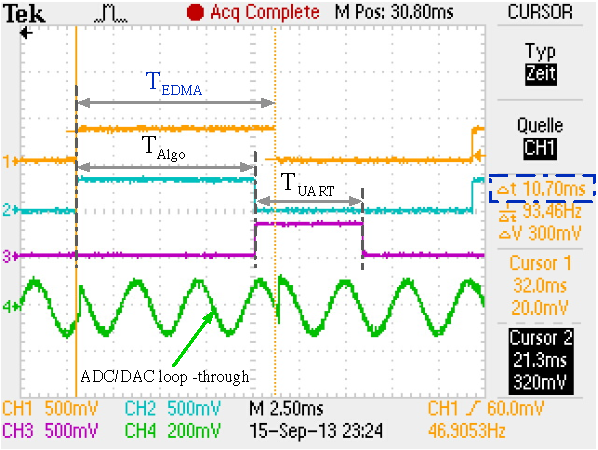
\includegraphics[width=\textwidth]{images/04_Echtzeitversuch/Profile_UART_9600}
                \caption{Baudrate: 9600 Baud}
                \label{fig:Profile_UART_9600}
        \end{subfigure}
        ~ %add desired spacing between images, e. g. ~, \quad, \qquad etc.
          %(or a blank line to force the subfigure onto a new line)
        \begin{subfigure}[b]{0.6\textwidth}
                \centering
                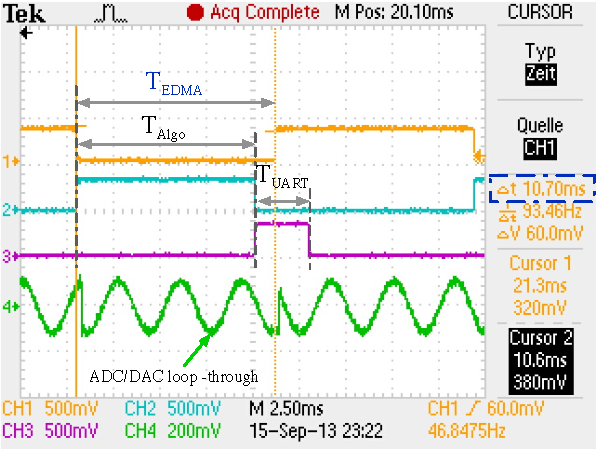
\includegraphics[width=\textwidth]{images/04_Echtzeitversuch/Profile_UART_19200}
                \caption{Baudrate: 19200 Baud}
                \label{fig:Profile_UART_19200}
        \end{subfigure}
        ~ %add desired spacing between images, e. g. ~, \quad, \qquad etc.
          %(or a blank line to force the subfigure onto a new line)
        \begin{subfigure}[b]{0.6\textwidth}
                \centering
                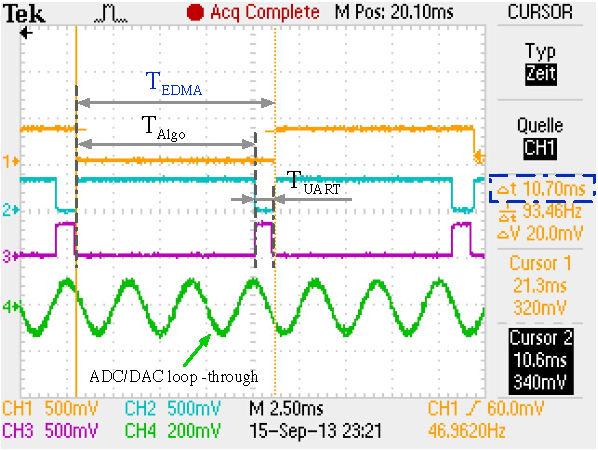
\includegraphics[width=\textwidth]{images/04_Echtzeitversuch/Profile_UART_57600}
                \caption{Baudrate: 57600 Baud}
                \label{fig:Profile_UART_57600}
        \end{subfigure}
        \caption{Untersuchung des Zeitverhaltens mit einer EDMA-Dauer von $T_{EDMA} = 10,7ms$.}
        \label{fig:profiling}
\end{figure}
% ----------------------------------------- SUB-FIGURE -----------------------------------












% ****************************************************************************************
\section{Versuchsaufbau}
\label{sec:Versuchsaufbau}
% ****************************************************************************************
\abb{aufbau_echtzeitmessung} zeigt den schematischen Versuchsaufbau der Echtzeitmessung. Um die Leistung des Systems in akustisch anspruchsvoller Umgebung testen zu können, wurde ein kleiner Raum mit den Abmaßen  $5m \times 3m \times 2,7m$ gewählt. Dieser verfügt über schallharte Wände, so dass die Systemreaktion auf ein diffuses Schallfeld sowie starke Reflexionen untersucht werden können. Zur Einhaltung des in \Sec{subsubsec:Fernfeld} beschriebenen Fernfeldkriteriums bei einer oberen Spracheckfrequenz von 3 kHz wurde ein Abstand von 1,6m gewählt. Zur Einstellung der unterschiedlichen Winkel wird das Array wie in \abb{array_winkeleinteilung} dargestellt drehbar gelagert und erhält ein Winkelaufteilung. Das Array kann so mit Hilfe des \ccs Graph-Windows exakt ausgerichtet werden und anhand der Winkelteilung in genauen Schritten gedreht werden.


\myFigure{real}                  % Figure tag (missing, real)
         {Big}                 % Size (small,medium,big)
         {h!}             % z.B. htbp
         {Versuchsaufbau der Echtzeitmessung}                % Figure title
         {aufbau_echtzeitmessung}                % Figure label 
         {04_Echtzeitversuch/aufbau_echtzeitmessung}     % Path to real figure





\myFigure{real}                  % Figure tag (missing, real)
         {medium}                 % Size (small,medium,big)
         {h!}                     % z.B. htbp
         {Einstellung der theoretischen Winkel am Mikrofonarray}                % Figure title
         {array_winkeleinteilung}                % Figure label 
         {04_Echtzeitversuch/array_winkeleinteilung}     % Path to real figure



% ****************************************************************************************
\section{Ergebnisse}
\label{sec:Ergebnisse}
% ****************************************************************************************
Im Folgenden wird zunächst ein grundlegender Funktionstest des Algorithmus durchgeführt. Anschließend erfolgt eine Verifikation der Winkelauflösung. Auf Grund der hohen Anzahl von Raumwinkelkombinationen werden im Rahmen dieses Tests nur einige ausgewählt, so dass eine Tendenz sichtbar werden kann.




% ****************************************************************************************
\subsection{Funktionstest}
\label{subsec:Funktionstest}
% ****************************************************************************************
Zum grundlegenden Test der Algorithmusfunktionalität wurden, wie in \abb{test_echtzeit_grundfunktion} dargestellt, vier verschiedene Schalleinfallsrichtungen eingestellt. Als Quellsignal diente eine Testdatei mit männlicher Sprache. Die Einstellungen der Histogrammglättung wurden mit einer Ringspeicherlänge von 20 und einer Schwelle von 20\% vorgenommen.

Es ist zunächst zu erkennen, dass der Algorithmus die Raumwinkel sicher detektiert. Auf Grund der endlich genauen Möglichkeit das Array zum Lautsprecher auszurichten, kann davon ausgegangen werden, dass Winkelfehler von einem Auflösungsschritt auf diese Einstellungstoleranz zurückzuführen sind. Die darüber hinaus auftretenden starken Winkelsprünge können den durch die Raumwände verursachten Reflexionen zugeschrieben werden. 
          


% ----------------------------------------- SUB-FIGURE -----------------------------------
\begin{figure}
        \centering
        \begin{subfigure}[b]{0.48\textwidth}
                \centering
                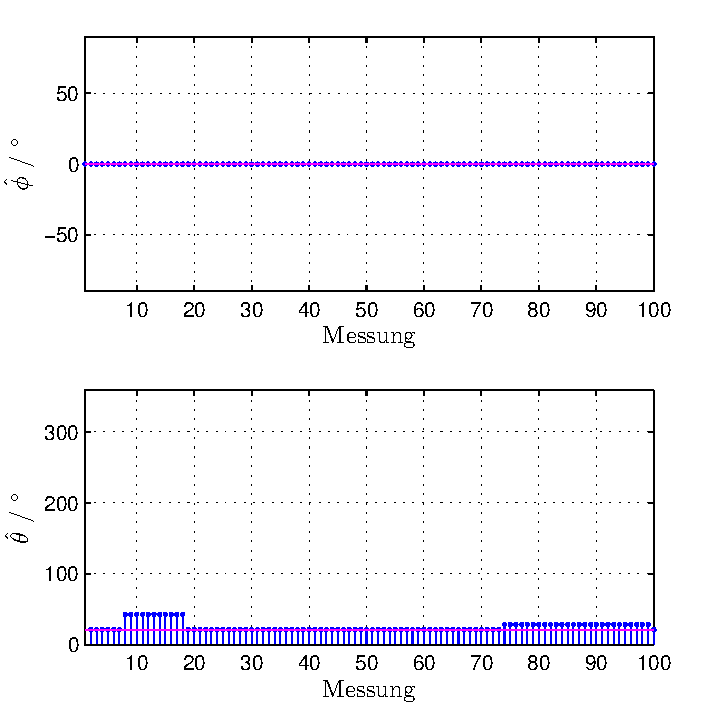
\includegraphics[width=\textwidth]{images/04_Echtzeitversuch/MALE_Phi_0_Theta_21}
                \label{fig:Foto_DSP_Draufsicht_Seitanansicht}
                \caption{$\phi=0°, \theta = 21°$}
        \end{subfigure}
        ~ %add desired spacing between images, e. g. ~, \quad, \qquad etc.
          %(or a blank line to force the subfigure onto a new line)
        \begin{subfigure}[b]{0.48\textwidth}
                \centering
                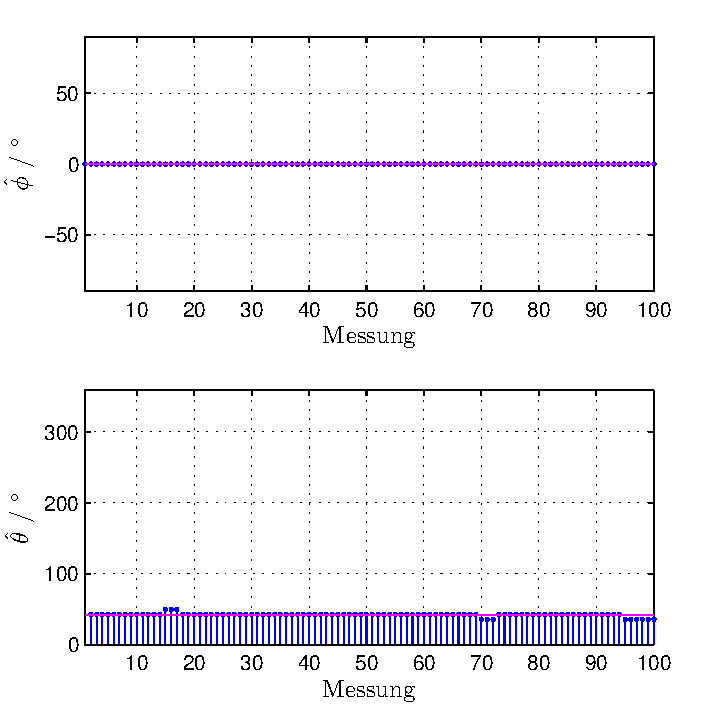
\includegraphics[width=\textwidth]{images/04_Echtzeitversuch/MALE_Phi_0_Theta_42}
                \label{fig:Foto_DSP_Draufsicht}
                \caption{$\phi=0°, \theta = 42°$}
        \end{subfigure}
        ~ %add desired spacing between images, e. g. ~, \quad, \qquad etc.
          %(or a blank line to force the subfigure onto a new line)
        \begin{subfigure}[b]{0.48\textwidth}
                \centering
                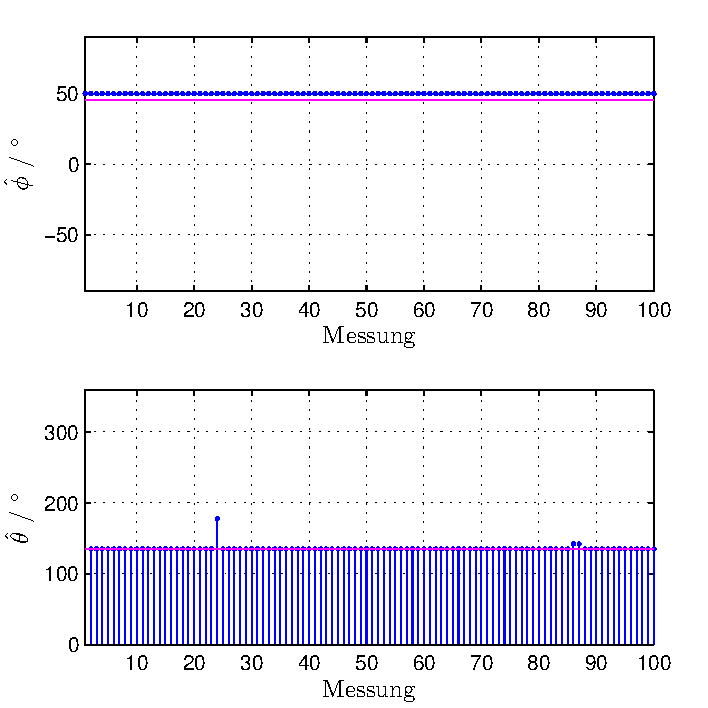
\includegraphics[width=\textwidth]{images/04_Echtzeitversuch/MALE_Phi_45_Theta_135}
                \label{fig:Foto_DSP_Draufsicht}
                \caption{$\phi=45°, \theta = 135°$}
        \end{subfigure}
        ~ %add desired spacing between images, e. g. ~, \quad, \qquad etc.
          %(or a blank line to force the subfigure onto a new line)
        \begin{subfigure}[b]{0.48\textwidth}
                \centering
                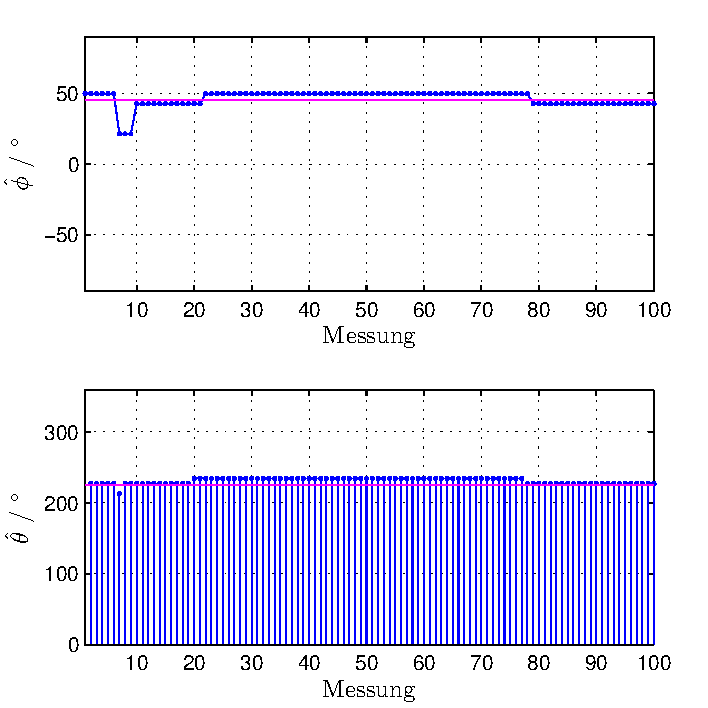
\includegraphics[width=\textwidth]{images/04_Echtzeitversuch/MALE_Phi_45_Theta_225}
                \label{fig:Foto_DSP_Draufsicht}
                \caption{$\phi=45°, \theta = 225°$}
        \end{subfigure}
        \stepcounter{missingFigureCount}
        \caption{Messung der Schalleinfallsrichtung aus unterschiedlichen Winkeln in einem hallenden Raum.}
        \label{fig:test_echtzeit_grundfunktion}
\end{figure}
% ----------------------------------------- SUB-FIGURE -----------------------------------



% ****************************************************************************************
\subsection{Verifikation der Winkelauflösung}
\label{subsec:VerifikationWinkelaufloesung}
% ****************************************************************************************
Zur Verifikation der Winkelauflösung wird das Mikrofonarray zunächst auf $\phi=0°$ und $\theta=0°$ ausgerichtet. Anschließend erfolgt eine Rotation um $\theta$ in Abständen der Winkelauflösung. Der Winkel $\theta$ wird dabei die Werte $0° \leq \theta \leq 92°$ annnehmen.
 
\abb{verifikation_winkelaufloesung_1} und \abb{verifikation_winkelaufloesung_2} illustrieren die Messergebnisse bei einer Anzahl von 100 Messungen pro Winkel. Hier wird ersichtlich, dass die Winkel im Abstand der in  \Sec{subsubsec:Winkelaufloesung} beschriebenen Winkelauflösung eingenommen werden können. Die Abweichungen um einen Winkelschritt sind erneut auf die begrenzte Einstellgenauigkeit zurückzuführen. Auf Grund von Reflexion ergeben sich hier erneut vereinzelte Fehler in Form von abrupten Winkelsprüngen.


% ----------------------------------------- SUB-FIGURE -----------------------------------
\begin{figure}
        \centering
        \begin{subfigure}[b]{0.48\textwidth}
                \centering
                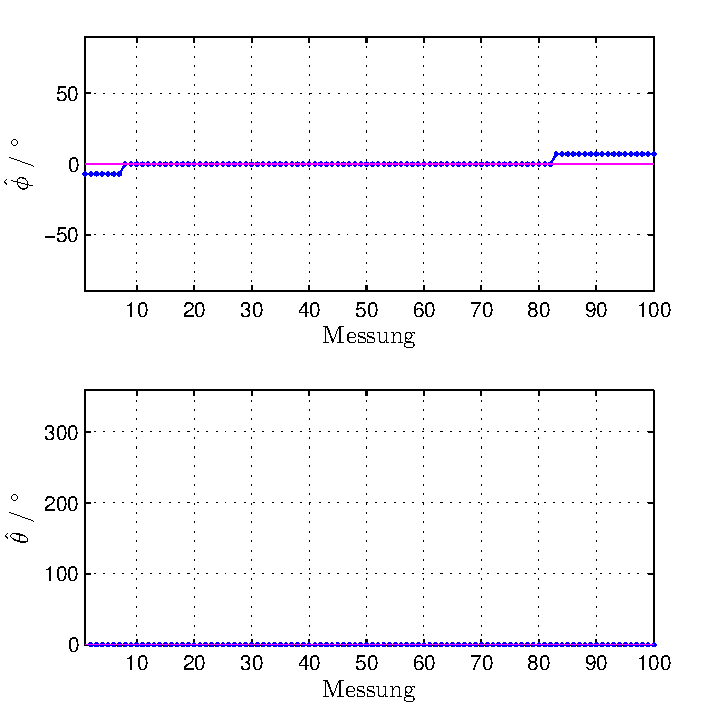
\includegraphics[width=\textwidth]{images/04_Echtzeitversuch/MALE_Phi_0_Theta_0}
                \label{fig:Foto_DSP_Draufsicht_Seitanansicht}
                \caption{$\phi=0°, \theta = 0°$}
        \end{subfigure}
        ~ %add desired spacing between images, e. g. ~, \quad, \qquad etc.
          %(or a blank line to force the subfigure onto a new line)
        \begin{subfigure}[b]{0.48\textwidth}
                \centering
                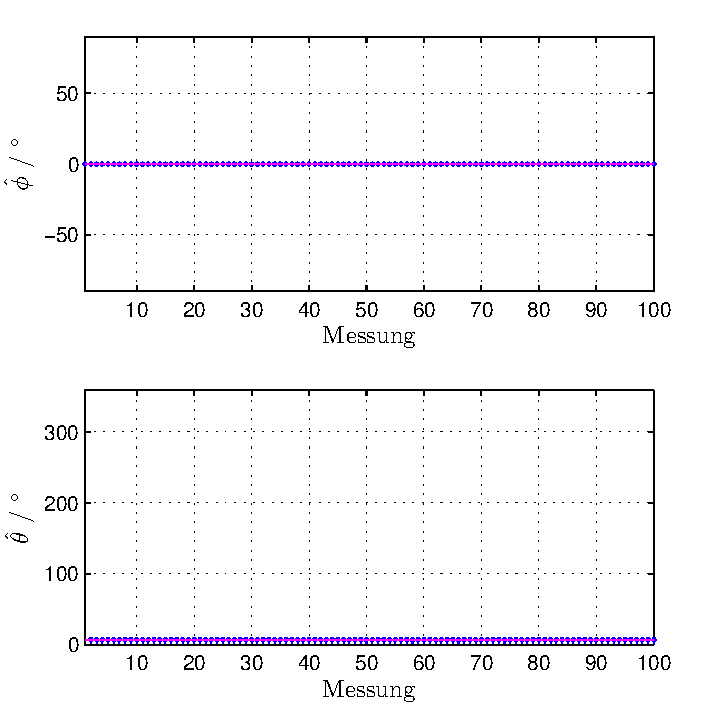
\includegraphics[width=\textwidth]{images/04_Echtzeitversuch/MALE_Phi_0_Theta_7}
                \label{fig:Foto_DSP_Draufsicht}
                \caption{$\phi=0°, \theta = 7°$}
        \end{subfigure}
        ~ %add desired spacing between images, e. g. ~, \quad, \qquad etc.
          %(or a blank line to force the subfigure onto a new line)
        \begin{subfigure}[b]{0.48\textwidth}
                \centering
                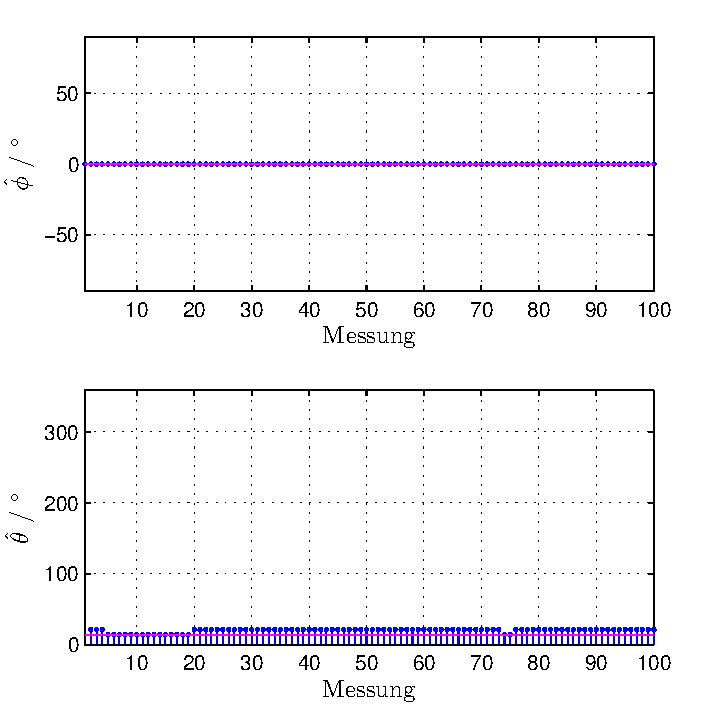
\includegraphics[width=\textwidth]{images/04_Echtzeitversuch/MALE_Phi_0_Theta_14}
                \label{fig:Foto_DSP_Draufsicht}
                \caption{$\phi=0°, \theta = 14°$}
        \end{subfigure}
        ~ %add desired spacing between images, e. g. ~, \quad, \qquad etc.
          %(or a blank line to force the subfigure onto a new line)
        \begin{subfigure}[b]{0.48\textwidth}
                \centering
                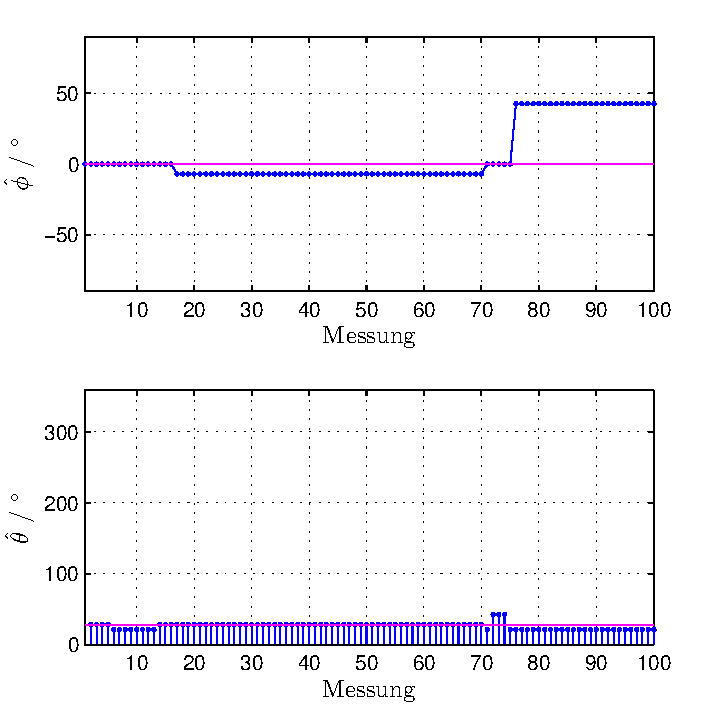
\includegraphics[width=\textwidth]{images/04_Echtzeitversuch/MALE_Phi_0_Theta_28}
                \label{fig:Foto_DSP_Draufsicht}
                \caption{$\phi=0°, \theta = 28°$}
        \end{subfigure}
         ~ %add desired spacing between images, e. g. ~, \quad, \qquad etc.
          %(or a blank line to force the subfigure onto a new line)
        \begin{subfigure}[b]{0.48\textwidth}
                \centering
                \includegraphics[width=\textwidth]{images/04_Echtzeitversuch/MALE_Phi_0_Theta_35}
                \label{fig:Foto_DSP_Draufsicht}
                \caption{$\phi=0°, \theta = 35°$}
        \end{subfigure}
        ~ %add desired spacing between images, e. g. ~, \quad, \qquad etc.
          %(or a blank line to force the subfigure onto a new line)
        \begin{subfigure}[b]{0.48\textwidth}
                \centering
                \includegraphics[width=\textwidth]{images/04_Echtzeitversuch/MALE_Phi_0_Theta_49}
                \label{fig:Foto_DSP_Draufsicht}
                \caption{$\phi=0°, \theta = 49°$}
        \end{subfigure}
        \stepcounter{missingFigureCount}
        \caption{Verifikation der Winkelauflösung im Bereich $0° \leq \theta \leq 49°$.}
        \label{fig:verifikation_winkelaufloesung_1}
\end{figure}
% ----------------------------------------- SUB-FIGURE -----------------------------------









% ----------------------------------------- SUB-FIGURE -----------------------------------
\begin{figure}
        \centering
        \begin{subfigure}[b]{0.48\textwidth}
                \centering
                \includegraphics[width=\textwidth]{images/04_Echtzeitversuch/MALE_Phi_0_Theta_56}
                \label{fig:Foto_DSP_Draufsicht_Seitanansicht}
                \caption{$\phi=0°, \theta = 56°$}
        \end{subfigure}
        ~ %add desired spacing between images, e. g. ~, \quad, \qquad etc.
          %(or a blank line to force the subfigure onto a new line)
        \begin{subfigure}[b]{0.48\textwidth}
                \centering
                \includegraphics[width=\textwidth]{images/04_Echtzeitversuch/MALE_Phi_0_Theta_63}
                \label{fig:Foto_DSP_Draufsicht}
                \caption{$\phi=0°, \theta = 63°$}
        \end{subfigure}
        ~ %add desired spacing between images, e. g. ~, \quad, \qquad etc.
          %(or a blank line to force the subfigure onto a new line)
        \begin{subfigure}[b]{0.48\textwidth}
                \centering
                \includegraphics[width=\textwidth]{images/04_Echtzeitversuch/MALE_Phi_0_Theta_71}
                \label{fig:Foto_DSP_Draufsicht}
                \caption{$\phi=0°, \theta = 71°$}
        \end{subfigure}
        ~ %add desired spacing between images, e. g. ~, \quad, \qquad etc.
          %(or a blank line to force the subfigure onto a new line)
        \begin{subfigure}[b]{0.48\textwidth}
                \centering
                \includegraphics[width=\textwidth]{images/04_Echtzeitversuch/MALE_Phi_0_Theta_78}
                \label{fig:Foto_DSP_Draufsicht}
                \caption{$\phi=0°, \theta = 78°$}
        \end{subfigure}
         ~ %add desired spacing between images, e. g. ~, \quad, \qquad etc.
          %(or a blank line to force the subfigure onto a new line)
        \begin{subfigure}[b]{0.48\textwidth}
                \centering
                \includegraphics[width=\textwidth]{images/04_Echtzeitversuch/MALE_Phi_0_Theta_85}
                \label{fig:Foto_DSP_Draufsicht}
                \caption{$\phi=0°, \theta = 85°$}
        \end{subfigure}
        ~ %add desired spacing between images, e. g. ~, \quad, \qquad etc.
          %(or a blank line to force the subfigure onto a new line)
        \begin{subfigure}[b]{0.48\textwidth}
                \centering
                \includegraphics[width=\textwidth]{images/04_Echtzeitversuch/MALE_Phi_0_Theta_92}
                \label{fig:Foto_DSP_Draufsicht}
                \caption{$\phi=0°, \theta = 92°$}
        \end{subfigure}
        \stepcounter{missingFigureCount}
        \caption{Verifikation der Winkelauflösung im Bereich $56° \leq \theta \leq 92°$.}
        \label{fig:verifikation_winkelaufloesung_2}
\end{figure}
% ----------------------------------------- SUB-FIGURE -----------------------------------



	% ****************************************************************************************
\chapter{Zusammenfassung}
\label{chap:Zusammenfassung}
% ****************************************************************************************
In der vorliegenden Arbeit wurde auf Basis des Mehrkanal-Kreuzkorrelations-koeffizienten ein System entwickelt, das in der Lage ist, eine bewegte Sprachquelle innerhalb eines Raumes zu detektieren. Als grundlegende Voraussetzung galt hier die Anwendung der Model-Based-Development-Methode\footnote{Modellgetriebene Softwareentwicklung}, in der zunächst ein umfassendes mathematisches Modell entwickelt, simuliert und anschließend auf einer entsprechenden Hardware realisiert wird. Die gesamte Modellierung wurde dabei mit der Entwicklungsumgebung \matlab erstellt. Die anschließende Realisierung erfolgte auf Basis von Hardware der Firma \ti sowie dessen Programmierumgebung \ccs.


Der hier implementierte Algorithmus lässt sich in folgende Teilschritte auflisten:

\begin{enumerate}
    \item Energieberechnung des Eingangssignals zur Klassifizierung des Signalblocks (stimmhaft, stimmlos)
    \item Kreuzkorrelation aller Eingangssignale unter Verwendung der von \ti zur Verfügung gestellten DSP-Bibliothek
    \item Verwendung der Korrelationsfunktionen zur räumlichen Suche/Detektion der Sprachquelle
    \item Ergebnisglättung unter Verwendung eines Histogramms
    \item Versenden der Ergebnisse mit Hilfe der serielle Schnittstelle
\end{enumerate}

Zur Einstellung der benötigten Systemparameter wurden zunächst entsprechende theoretische Überlegungen getätigt. Beim anschließenden Echtzeittest wurde allerdings festgestellt, dass die Energieschwelle, die Länge des Histogrammspeichers und dessen Schwelle abhängig von den gegebenen Raumeigenschaften empirisch ermittelt werden mussten.

Neben der Entwicklung des Detektionsalgorithmus wurde darüber hinaus ein räumliches Mikrofonarray entworfen sowie gefertigt. Mit Hilfe des simplen Steckmechanismus konnte diese aufwandsarm sowie kostengünstig mit einer hohen Fertigungsgenauigkeit hergestellt werden. Des Weiteren ist es möglich, auf Grund des einfachen Klipp-Systems die empfindlichen Mikrofonkapseln der Forma \sennheiser unkompliziert zu entfernen und anderweitig einzusetzen. 


% ****************************************************************************************
\section{Bewertung der Ergebnisse}
\label{sec:BewertungErgebnisse}
% ****************************************************************************************
Zur Bewertung der erzielten Ergebnisse werden zunächst die in \Chap{Einfuehrung} genannten Forderungen diskutiert.


\paragraph{Verarbeitung von Sprachsignalen} - Der Algorithmus ist in der Lage, ein breitbandiges Sprachsignal zu verarbeiten da die Raumwinkel durch Analyse der Redundanz zwischen den einzelnen Mikrofonsignalen ermittelt werden. Auf Grund dessen ist das Schätzergebnis grundsätzlich unabhängig von den im Signal enthaltenen Frequenzen.


\paragraph{Winkelauflösung} - Die Winkelauflösung ist lediglich abhängig von der Abtastfrequenz und kann im Hinblick auf das Auftreten des räumlichen Aliasing-Effekts nicht durch Vergrößerung der Array-Dimension erhöht werden. Auf Grund der rechenintesieven Operationen ist eine Erhöhung der Abtastfrequenz und somit der Winkelauflösung nur dich eine Erhöhung der zur Verfügung stehenden CPU-Taktschritte möglich. Diesbezüglich kann die hier erreichte Winkelauflösung durch ausreichend betrachtet werden. Während der Durchführung des Echtzeittests konnte jede Signalquelle auch bei kleinen Ortsänderungen verfolgt werden.  


\paragraph{Rechenzeit} - Auf Grund der durch die EDMA-Blocklänge sowie die durch die Abtastfrequenz festgelegten maximalen Rechendauer musste ein Verfahren entwickelt werden, das in der Lange ist, den Raum erst in groben und anschließend sukzessiv in immer kleiner werdenden Winkelschritten abzusuchen. Obwohl durch diese Methode das Echtzeitkriterium erzielt wird, ergeben sich fehlerhaft erkannte Winkel bis hin zu kleinen Bereiche, an denen keine Position erkennt werden kann. Eine weitere Optimierung des Systems müsste dann an dieser Stelle fortgeführt werden.


\paragraph{Winkelraum} - Im Vergleich zu den Arbeiten \cite{Master_Array_Pikora}
 und \cite{Master_Array_Mueller}, in denen auf Grund der Arraygeometrie nur ein eingeschränkter Winkelbereich abgedeckt werden konnte, erzielt das hier entwickelte System sehr gute Ergebnisse. Auf Grund der räumlichen Arraygeometrie kann jeder Raumwinkel im Raster der Winkelauflösung abgebildet werden.
 
 

Beim Betrachten des gesamten Projekts im Überblick wird ersichtlich, dass eine Methode gefunden wurde um mit Hilfe eines Acht-Kanal-Mikrofonarrays eine Sprachquelle im Raum zu detektieren. Die erzielten Messergebnisse des Echtzeitsystems in der ersten Version zeigen eine deutliche Tendenz. Zur Implementierung des Systems in einer realen Anwendung sind weiterführende Schritte notwendig, da hier die zwingende Notwendigkeit fehlerfreier Ergebnisse vorliegt.



% ****************************************************************************************
\section{Ausblick}
\label{sec:Ausblick}
% ****************************************************************************************
Auf Grundlage dieser Arbeit könnte versucht werden, die Winkelauflösung durch sukzessive Signalinterpolation zu erhöhen. Dazu müsste zunächst die Schalleinfallsrichtung für eine fest eingestellte Winkelauflösung ermittelt werden. Anschließend könnte entsprechend dieser Quellenrichtung ein kürzeres Signalstück entnommen, interpoliert und erneut auf die Schalleinfallsrichting untersucht werden.

Des Weiteren bestünde die Möglichkeit zur Untersuchung auf die Systemreaktion unter Verwendung der GCC-PHAT und deren Robustheit bei der Verwendung von Sprachsignalen. 

Im Hinblick auf das realisierte Kreuzpeilungssystem in \citet{Master_Array_Mueller} könnte dieses um eine Dimension erweitert werden und Signalquellen im Raum peilen.











%--------------------------------------------------------------------------
% Literaturverzeichnis
%--------------------------------------------------------------------------
	% Anpassung an deutsche Zitierweise, Alphabetische Sortierung, Abkürzungen
	\bibliographystyle{dinat}
	

	% Literaturverzeichnis
	\bibliography{literatur/literatur}

%--------------------------------------------------------------------------
% Anhänge
%--------------------------------------------------------------------------
	%\appendix
        %% Codierung: Larin1

% ****************************************************************************************
\chapter{Kreuzkorrelation periodischer Signale}
\label{appx:KreuzkorrelationPeriodischerSignale} 
% ****************************************************************************************
Die Kreuzkorrelation zweier periodischer Signale der Form $x(t)=\cos(2\pi ft)$ und  $y(t) = \cos(2\pi f (t+\Delta t))$ liefert:

\begin{equation}
\label{eq:KorrPeriodisch1}
r_{xy}(\tau) =\frac{1}{T} \int_{0}^{T} \cos(2\pi ft) \cdot \cos(2\pi f (t+\Delta t+\tau)) \mathrm dt
\end{equation}

Mit Verwendung der trigonometrischen Identität $\cos(\alpha) \cdot \cos(\beta) = \frac{1}{2}\left(\cos(\alpha - \beta) - \cos(\alpha + \beta)\right)$ folgt:

\begin{equation}\label{eq:KorrPeriodisch2}
    \begin{split}
r_{xy}(\tau) = \frac{1}{T} \int_{0}^{T} & \frac{1}{2} ( \cos{(2\pi ft - 2\pi f (t+\Delta t+\tau))} \\ & - \cos{(2\pi ft + 2\pi f (t+\Delta t+\tau))} ) \mathrm dt
    \end{split}
\end{equation}

Nach Vereinfachung durch zusammenfassen ergibt sich des weiteren:

\begin{equation}
\label{eq:KorrPeriodisch3}
r_{xy}(\tau) = \frac{1}{2T} \cdot \cos{(2\pi f (\Delta t+\tau))} + \underbrace{\int_{0}^{T}  \cos(4\pi ft - 2\pi f (\Delta t+\tau))\mathrm dt}_{0}
\end{equation}

Der erste Term in \Eq{KorrPeriodisch2} kann aus dem Integral entfernt werden da keine Abhängigkeit zur Integrationsvariable $t$ mehr besteht. Die Integration des zweiten Terms über eine gesamte Periode $T$ liefert das Ergebnis Null da sich positive und negative Halbwellen der Cosinus-Funktion auslöschen. Als Ergebnis bleibt:

\begin{equation}
\label{eq:KorrPeriodisch4}
r_{xy}(\tau) = \frac{1}{2T} \cdot \cos(2\pi f (\Delta t+\tau))
\end{equation}

Die Kreuzkorrelation periodischer Signale liefert nach \Eq{KorrPeriodisch4} eine ebenfalls periodische Kreuzkorrelationsfunktion $r_{xy}(\tau)$.
													% dieser Arbeit
%	\input{anhang/quellcode/quellcode}				% Anhang B: Quellcode
%--------------------------------------------------------------------------
% Glossar
%--------------------------------------------------------------------------
	\printnomenclature
%--------------------------------------------------------------------------
% Stichwortverzeichnis
%--------------------------------------------------------------------------
	\printindex
%--------------------------------------------------------------------------
% Erklärung über Selbstständigkeit
%--------------------------------------------------------------------------
%	\asurency
%--------------------------------------------------------------------------
\end{document}
